%% USPSC-modelo-EESC.tex
% ---------------------------------------------------------------
% USPSC: Modelo de Trabalho Acadêmico (tese de doutorado, dissertacao de
% mestrado e trabalhos monograficos em geral) em conformidade com 
% ABNT NBR 14724:2011: Informação e documentação - Trabalhos acadêmicos -
% Apresentação
%----------------------------------------------------------------
%% Esta é uma customização do abntex2-modelo-trabalho-academico.tex de v-1.9.5 laurocesar 
%% para as Unidades do Campus USP de São Carlos:
%% EESC - Escola de Engenharia de São Carlos
%% IAU - Instituto de Arquitetura e Urbanismo
%% ICMC - Instituto de Ciências Matemáticas e de Computação
%% IFSC - Instituto de Física de São Carlos
%% IQSC - Instituto de Química de São Carlos
%%
%% Este trabalho utiliza a classe USPSC (USPSC.cls e USPSC1.cls) que é mantida 
%% pela seguinte equipe:
%% 
%% Coordenação e Programação:
%%   - Marilza Aparecida Rodrigues Tognetti - marilza@sc.usp.br (PUSP-SC)
%%   - Ana Paula Aparecida Calabrez - aninha@sc.usp.br (PUSP-SC)
%% Normalização:
%%   - Brianda de Oliveira Ordonho Sigolo - brianda@usp.br (IAU)
%%   - Eduardo Graziosi Silva - edu.gs@sc.usp.br (EESC)
%%   - Eliana de Cássia Aquareli Cordeiro - eliana@iqsc.usp.br (IQSC)
%%   - Flávia Helena Cassin - cassinp@sc.usp.br (EESC)
%%   - Maria Cristina Cavarette Dziabas - mcdziaba@ifsc.usp.br (IFSC)
%%   - Regina Célia Vidal Medeiros - rcvmat@icmc.usp.br (ICMC)
%%
%% Os modelos desenvolvidos utilizam diversos arquivos relacionado em 
%% 2.1 Pacote USPSC: Classe USPSC e modelos de trabalhos acadêmicos	do Tutorial do Pacote 
%%  USPSC para modelos de trabalhos de acadêmicos em LaTeX - versão 3.2

%----------------------------------------------------------------
%% Sobre a classe abntex2.cls:
%% abntex2.cls, v-1.9.5 laurocesar
%% Copyright 2012-2015 by abnTeX2 group at https://www.abntex.net.br/ 
%%
%----------------------------------------------------------------

\documentclass[
% -- opções da classe memoir --
12pt,		% tamanho da fonte
openright,	% capítulos começam em pág ímpar (insere página vazia caso preciso)
twoside,  % para impressão em anverso (frente) e verso. Oposto a oneside - Nota: utilizar \imprimirfolhaderosto*
%oneside, % para impressão em páginas separadas (somente anverso) -  Nota: utilizar \imprimirfolhaderosto
% inclua uma % antes do comando twoside e exclua a % antes do oneside 
a4paper,			% tamanho do papel. 
% -- opções da classe abntex2 --
chapter=TITLE,		% títulos de capítulos convertidos em letras maiúsculas
% -- opções do pacote babel --
english,			% idioma adicional para hifenização
french,				% idioma adicional para hifenização
spanish,			% idioma adicional para hifenização
brazil				% o último idioma é o principal do documento
% {USPSC-classe/USPSC} configura o cabeçalho contendo apenas o número da página
]{USPSC-classe/USPSC}
%]{USPSC-classe/USPSC1}
% Inclua % antes de ]{USPSC-classe/USPSC} e retire a % antes de %]{USPSC-classe/USPSC1} para utilizar o 
% cabeçalho diferenciado para as páginas pares e ímpares:
%- páginas ímpares: com seções ou subseções e o número da página
%- páginas pares: com o número da página e o título do capítulo 
% ---
% ---
% Pacotes básicos - Fundamentais 
% ---
\usepackage[T1]{fontenc}		% Seleção de códigos de fonte.
\usepackage[utf8]{inputenc}		% Codificação do documento (conversão automática dos acentos)
\usepackage{lmodern}			% Usa a fonte Latin Modern
% Para utilizar a fonte Times New Roman, inclua uma % no início do comando acima  "\usepackage{lmodern}"
% Abaixo, tire a % antes do comando  \usepackage{times}
%\usepackage{times}		    	% Usa a fonte Times New Roman	
% Para usar a fonte , lembre-se de tirar a % do comando %\renewcommand{\ABNTEXchapterfont}{\rmfamily}, localizado mais abaixo, logo após "Outras opções para nota de rodapé no Sistema Numérico" 						
\usepackage{lastpage}			% Usado pela Ficha catalográfica
\usepackage{indentfirst}		% Indenta o primeiro parágrafo de cada seção.
\usepackage{color}				% Controle das cores
\usepackage{graphicx}			% Inclusão de gráficos
\usepackage{float} 				% Fixa tabelas e figuras no local exato
\usepackage{chemfig}            % Para escrever reações químicas
\usepackage{chemmacros}         % Para escrever reações químicas
\usepackage{tikz}				% Para escrever reações químicas e outros
\usetikzlibrary{positioning}
\usepackage{microtype} 			% para melhorias de justificação
\usepackage{pdfpages}
\usepackage{makeidx}            % para gerar índice remissivo
\usepackage{hyphenat}          % Pacote para retirar a hifenizacao do texto
\usepackage[absolute]{textpos} % Pacote permite o posicionamento do texto
\usepackage{eso-pic}           % Pacote para incluir imagem de fundo
\usepackage{makebox}           % Pacote para criar caixa de texto
% ---

\usepackage{amsmath}     % Recursos avançados de fórmulas matemáticas
\usepackage{amssymb}     % Símbolos matemáticos adicionais (da AMS)
\usepackage{amsfonts}    % Fontes matemáticas da AMS (como \mathbb)
\usepackage{amsthm}      % Ambientes de teorema, proposição, lema, etc.
\usepackage{mathtools}   % Extensão do amsmath (melhora alinhamento e símbolos)
\usepackage{bm}          % Negrito em símbolos matemáticos (como vetores)
\usepackage{eufrak}      % Fonte gótica para notações matemáticas especiais
\usepackage{mathrsfs}    % Fonte caligráfica elegante (usada em notação de conjuntos)
\usepackage{xfrac}       % Frações inclinadas (por exemplo, ½)
\usepackage{gensymb}     % Símbolos gerais (°, ′, ″, etc.)
\usepackage{subeqnarray} % Numeração de subequações (1a, 1b, ...)
\usepackage{cancel}      % Permite riscar termos em equações (ex: \cancel{x})
\usepackage{algorithm}          % Cria o ambiente de algoritmo (flutuante, numerado)
\usepackage{algpseudocode}      % Comandos de pseudocódigo (If, For, While, etc.)
\usepackage[caption=false]{subfig}


\makeatletter
\providecommand*{\subfigureautorefname}{\figurename}
\makeatother

\makeatletter
\renewcommand{\ALG@name}{Algoritmo}
\makeatother

% Algoritmos com Declaracoes em Português
\algrenewcommand\algorithmicend{\textbf{fim}}
\algrenewcommand\algorithmicdo{\textbf{faça}}
\algrenewcommand\algorithmicrequire{\textbf{Requer}}
\algrenewcommand\algorithmicwhile{\textbf{enquanto}}
\algrenewcommand\algorithmicfor{\textbf{para}}
\algrenewcommand\algorithmicif{\textbf{se}}
\algrenewcommand\algorithmicthen{\textbf{então}}
\algrenewcommand\algorithmicelse{\textbf{senão}}
\algrenewcommand\algorithmicreturn{\textbf{devolve}}
\algrenewcommand\algorithmicfunction{\textbf{função}}
%
%% Rearranja os finais de cada estrutura
\algrenewtext{EndWhile}{\algorithmicend\ \algorithmicwhile}
\algrenewtext{EndFor}{\algorithmicend\ \algorithmicfor}
\algrenewtext{EndIf}{\algorithmicend\ \algorithmicif}
\algrenewtext{EndFunction}{\algorithmicend\ \algorithmicfunction}

%%%%%%%%%%%%%%%%%%%%%%%%%%%%%%%%%%%%%%%%%%%%%%%%%%%%%%%%%%
% GRUMEC
%%%%%%%%%%%%%%%%%%%%%%%%%%%%%%%%%%%%%%%%%%%%%%%%%%%%%%%%%%
%Lagrangian position (inital configuration) vector
\newcommand{\lPosition}{\mathbf{x}}
\newcommand{\lDomain}{_{\Omega}_x}
\newcommand{\lBoundary}{\Gamma_x}
%Eulerian position (current configuration) vector
\newcommand{\ePosition}{\mathbf{y}}
\newcommand{\eDomain}{\Omega_y}
\newcommand{\eBoundary}{\Gamma_y}
%rigth Cauchy-Green stretch tensor
\newcommand{\cauchyStretch}{\mathbf{C}}
\newcommand{\constitutiveTensor}{\mathbb{C}}
%Green-Lagrange strain tensor
\newcommand{\greenStrain}{\mathbf{E}}
\newcommand{\piolaStress}{\mathbf{S}}
\newcommand{\cauchyStress}{\bm{\sigma}}
%Configuration change function
\newcommand{\deformation}{\mathbfcal{F}}
\newcommand{\lDeformation}{\mathbfcal{F}_x^h}
\newcommand{\eDeformation}{\mathbfcal{F}_y^h}
\newcommand{\lMedDeformation}{\mathbfcal{F}_x^{mh}}
\newcommand{\eMedDeformation}{\mathbfcal{F}_y^{mh}}
%%Gradient of Configuration change function
\newcommand{\gradDeformation}{\mathbf{A}}
\newcommand{\lGradDeformation}{\mathbf{A}_x^h}
\newcommand{\eGradDeformation}{\mathbf{A}_y^h}
\newcommand{\lMedGradDeformation}{\mathbf{A}_x^{mh}}
\newcommand{\eMedGradDeformation}{\mathbf{A}_y^{mh}}
%%Maping to initial
\newcommand{\initDeformation}{\mathbfcal{F}_0}
%%Gradient of maping to initial
\newcommand{\gradInitDeformation}{\mathbf{A}_0}
\newcommand{\jacobianDeformation}{J}
%strain tensor
\newcommand{\straintensor}{\bm{\varepsilon}}

\newcommand{\totalEnergy}{\Pi}
\newcommand{\extEnergy}{\mathbb{P}}
\newcommand{\kinEnergy}{\mathbb{K}}
\newcommand{\intEnergy}{\mathbb{U}_e}
\newcommand{\concLoad}{\mathbf{F}}
\newcommand{\ebodyLoad}{\mathbf{b}}
\newcommand{\bodyLoad}{\mathbf{b}^0}
\newcommand{\tractionLoad}{\mathbf{p}}
\newcommand{\ltractionLoad}{\mathbf{p}^{0}}
\newcommand{\solidVel}{\dot{\mathbf{y}}}
\newcommand{\solidAccel}{\ddot{\mathbf{y}}}
\newcommand{\specificEnergy}{u_e}
\newcommand{\bulkModulus}{\kappa}
\newcommand{\shearModulus}{G}
\newcommand{\elasticModulus}{\mathbb{E}}
\newcommand{\lameParameter}{\lambda}
\newcommand{\SVKenergy}{u_e^{SVK}}

\newcommand{\intLoads}{\mathbf{F}^{int}}
\newcommand{\extLoads}{\mathbf{F}^{ext}}
\newcommand{\solidMass}{\mathbf{M}}
\newcommand{\solidDamping}{\mathbf{C}}
\newcommand{\solidHessian}{\mathbf{H}}

\newcommand{\SolidInitPos}{\mathbf{X}}
\newcommand{\SolidPos}{\mathbf{Y}}
\newcommand{\SolidVel}{\dot{\mathbf{Y}}}
\newcommand{\SolidAccel}{\ddot{\mathbf{Y}}}

\newcommand{\lGenVector}{\mathbf{g}_x}
\newcommand{\eGenVector}{\mathbf{g}_y}
\newcommand{\lUnitVector}{\mathbf{e}_x}
\newcommand{\eUnitVector}{\mathbf{e}_y}
\newcommand{\lThickness}{h_x}
\newcommand{\eThickness}{h_y}
\newcommand{\stRate}{a}
\newcommand{\lTheta}{\theta_x}
\newcommand{\eTheta}{\theta_y}
\newcommand{\NNSS}{\mathbf{R}_S}
\newcommand{\lGrad}{\boldsymbol{\nabla}_\mathbf{x}}


%%%%%%%%%%%%%%%%%%%%%%%%%%%%%%%%%%%%%%%%%%%%%%%%%%%%%%%%%%
% GRUMEC - TIME INTEGRATION
%%%%%%%%%%%%%%%%%%%%%%%%%%%%%%%%%%%%%%%%%%%%%%%%%%%%%%%%%%
%Alpha_f
\newcommand{\alphaf}{\alpha_f}
%alpha_m
\newcommand{\alpham}{\alpha_m}
%spectral radius
\newcommand{\specRadius}{\rho_\infty}
%time
\newcommand{\tempo}{t}
%time step
\newcommand{\timeStep}{\Delta t}
%initial velocity
\newcommand{\initialVelocity}{\mathbf{u}_s^h}
%Total time
\newcommand{\totalTime}{T}

%%%%%%%%%%%%%%%%%%%%%%%%%%%%%%%%%%%%%%%%%%%%%%%%%%%%%%%%%%
% GRUMEC - ARLEQUIN
%%%%%%%%%%%%%%%%%%%%%%%%%%%%%%%%%%%%%%%%%%%%%%%%%%%%%%%%%%
%Global model
\newcommand{\globalModel}{\Omega_0}
\newcommand{\globalBoundary}{\Gamma_0}
%Arlequin model
\newcommand{\arlqModel}{\Omega_i}
\newcommand{\arlqBoundary}{\Gamma_i}

%Local model
\newcommand{\localModel}{\Omega_1}
\newcommand{\localBoundary}{\Gamma_1}
%Gluing zone
\newcommand{\gluingZone}{\Omega_c}
%Free zone
\newcommand{\freeZone}{\Omega_{fr}}
%Overlapping Zone
\newcommand{\overlappingZone}{\Omega_s}
%Weighting function
\newcommand{\arlequinWF}{\alpha}
\newcommand{\arlequinWFi}{\alpha_i}
%weigthing function local model
\newcommand{\arlequinWFLocal}{\alpha_1}
%weighting function global model
\newcommand{\arlequinWFGlobal}{\alpha_0}

%local velocity
\newcommand{\ulocal}{\mathbf{u}_1}
\newcommand{\ulocalh}{\mathbf{u}_1^h}
%global velocity
\newcommand{\uglobal}{\mathbf{u}_0}
\newcommand{\uglobalh}{\mathbf{u}_0^h}
%velocity Arlequin from model i
\newcommand{\uArlqi}{\mathbf{u}_i^{h}}
%global velocity weight function
\newcommand{\wglobal}{\mathbf{w}_0}
\newcommand{\wglobalh}{\mathbf{w}_0^h}
%local velocity weight function
\newcommand{\wlocal}{\mathbf{w}_1}
%global velocity weight function
\newcommand{\wlocalh}{\mathbf{w}_1^h}
%velocity Arlequin weight function from model i
\newcommand{\wArlqi}{\mathbf{w}_i^h}

%global pressure
\newcommand{\pglobal}{p_0}
\newcommand{\pglobalh}{p_0^h}
%local pressure
\newcommand{\plocal}{p_1}
\newcommand{\plocalh}{p_1^h}
%pressure Alequin from model i
\newcommand{\pArlqi}{p_i^{h}}
%global pressure weight function
\newcommand{\qglobal}{q_0}
\newcommand{\qglobalh}{q_0^h}
%local pressure weight function
\newcommand{\qlocal}{q_1}
\newcommand{\qlocalh}{q_1^h}
%pressure Arlequin weight function from model i
\newcommand{\qArlqi}{q_i^h}

%Surface and body forces in each model
\newcommand{\globalSurfaceLoadh}{\mathbf{h}_0^h}
\newcommand{\localSurfaceLoadh}{\mathbf{h}_1^h}
\newcommand{\arlqSurfaceLoadh}{\mathbf{h}_i^h}
\newcommand{\globalsbodyforceh}{\mathbf{f}_0^h}
\newcommand{\localsbodyforceh}{\mathbf{f}_1^h}
\newcommand{\arlqsbodyforceh}{\mathbf{f}_i^h}

%Lagrange multiplier
\newcommand{\lagrangeMultiplier}{\boldsymbol{\lambda}}
\newcommand{\LagrangeMultiplier}{\boldsymbol{\Lambda}}
\newcommand{\lagrangeMultiplierh}{\boldsymbol{\lambda}^h}
%Lagrange multiplier weight function
\newcommand{\lagrangeMultiplierWF}{\boldsymbol{\zeta}}
\newcommand{\lagrangeMultiplierWFh}{\boldsymbol{\zeta}^h}

%Trial and test spaces
%Solution space global model - velocity
\newcommand{\uGlobalSolution}{\mathcal{S}_{u0}^h}
%Solution space local model - velocity
\newcommand{\uLocalSolution}{\mathcal{S}_{u1}^h}
%Solution space Arlequin model - velocity
\newcommand{\uArlequinSolution}{\mathcal{S}_{ui}^h}
%Solution space global model - velocity
\newcommand{\uGlobalTest}{\mathcal{V}_{u0}^h}
%Solution space global model - velocity
\newcommand{\uLocalTest}{\mathcal{V}_{u1}^h}
%Solution space Arlequin model - velocity
\newcommand{\uArlequinTest}{\mathcal{V}_{ui}^h}

%Solution space global model - pressure
\newcommand{\pGlobalSolution}{\mathcal{S}_{p0}^h}
%Solution space local model - pressure
\newcommand{\pLocalSolution}{\mathcal{S}_{p1}^h}
%Solution space Arlequin model - pressure
\newcommand{\pArlequinSolution}{\mathcal{S}_{pi}^h}
%Solution space global model - pressure
\newcommand{\pGlobalTest}{\mathcal{V}_{p0}^h}
%Solution space global model - pressure´
\newcommand{\pLocalTest}{\mathcal{V}_{p1}^h}
%Solution space Arlequin model - pressure
\newcommand{\pArlequinTest}{\mathcal{V}_{pi}^h}

%Solution space global model - lagrange multiplier
\newcommand{\lagSolution}{\mathcal{M}^h}
%Solution space global model - lagrange multiplier
\newcommand{\lagTest}{\mathcal{Q}^h}

%Arlequin Stabilization Parameter
\newcommand{\tauArlequin}{\tau_{ARLQ}}
\newcommand{\tauArlequini}{\tau_{ARLQi}}
\newcommand{\tauArlequinGlobal}{\tau_{ARLQ0}}
\newcommand{\tauArlequinLocal}{\tau_{ARLQ1}}
%Number of subdomains
\newcommand{\nSubDomains}{n_{dom}}

\newcommand{\resMomGlobal}{\mathbf{r}_{\mathrm{M0}}^{h}}
\newcommand{\resMomI}{\mathbf{r}_{\mathrm{Mi}}^{h}}
\newcommand{\resMomLocal}{\mathbf{r}_{\mathrm{M1}}^{h}}
\newcommand{\resPreGlobal}{r_{\mathrm{C0}}^{h}}
\newcommand{\resPreI}{r_{\mathrm{Ci}}^{h}}
\newcommand{\resPreLocal}{r_{\mathrm{C1}}^{h}}

\newcommand{\NNSL}{\mathrm{R}_\mathrm{L}}
\newcommand{\NNSMLocal}{\mathrm{R}_\mathrm{M1}}
\newcommand{\NNSMArlq}{\mathrm{R}_\mathrm{M,i}}
\newcommand{\NNSCLocal}{\mathrm{R}_\mathrm{C1}}
\newcommand{\NNSMGlobal}{\mathrm{R}_\mathrm{M0}}
\newcommand{\NNSCGlobal}{\mathrm{R}_\mathrm{C0}}
\newcommand{\NNSCArlq}{\mathrm{R}_\mathrm{C,i}}


%%%%%%%%%%%%%%%%%%%%%%%%%%%%%%%%%%%%%%%%%%%%%%%%%%%%%%%%%%
% MESH PROBLEM
%%%%%%%%%%%%%%%%%%%%%%%%%%%%%%%%%%%%%%%%%%%%%%%%%%%%%%%%%%
%Mesh Moving
\newcommand{\domaintt}{\Omega_{\tilde{t}}}
\newcommand{\testfunction}{\mathbf{w}^h}
\newcommand{\displacementmesh}{\bar{\mathbf{z}}^h}
\newcommand{\referencecoordinates} {\mathbf{X}^h}
\newcommand{\currentcoordinates} {\mathbf{y}^h}
\newcommand{\currentcoordinatessh} {\mathbf{y}}
\newcommand{\adimensionalcoordinates}{\boldsymbol{\xi}}
\newcommand{\error}{e_{L2}}
\newcommand{\stif}{\mathbf{K}}
\newcommand{\domainref}{\Omega_{ref}}

%%%%%%%%%%%%%%%%%%%%%%%%%%%%%%%%%%%%%%%%%%%%%%%%%%%%%%%%%%
% FLUID PROBLEM
%%%%%%%%%%%%%%%%%%%%%%%%%%%%%%%%%%%%%%%%%%%%%%%%%%%%%%%%%%

%mathematical commands
\newcommand{\trace}{\mathrm{tr}}
\newcommand{\unittensor}{\mathbf{I}}
\newcommand{\increment}{\varDelta}
\newcommand{\imaginary}{\imath}
\newcommand{\complexspace}{{\mathbb C}}
\newcommand{\laplacian}{\Delta}
\newcommand{\strainrate}{\boldsymbol{{\dot{\varepsilon}}}}
\newcommand{\strainratetensor}{\dot{\bm{\varepsilon}}}
\newcommand{\vzero}{\mathbf{0}}
\newcommand{\deriv}{\mathrm{d}}
\newcommand{\divergence}{\boldsymbol{\nabla_y}}
\newcommand{\gradient}{\boldsymbol{\nabla_y}}
\newcommand{\realspace}{\mathbb{R}}
\newcommand{\nrealspace}{\mathbb{R}^{\nsd}}


%fluid domain
%domain
\newcommand{\domain}{\Omega}
\newcommand{\domainh}{\Omega^h}
\newcommand{\domainT}{\Omega_t}
%element domain
\newcommand{\domainE}{\Omega^e}
%boundary
\newcommand{\boundary}{\Gamma}
\newcommand{\boundaryh}{\Gamma^h}
%Dirichlet boundary
\newcommand{\GammaD}{\Gamma_{D}}
%Neumann boundary
\newcommand{\GammaN}{\Gamma_{N}}
%boundary normal vectors^
\newcommand{\snormal}{\mathbf{n}}
\newcommand{\normal}{\mathbf{n}}
%ALE domains
\newcommand{\domainMat}{\Omega_{0}}
\newcommand{\domainRef}{\Omega_{\bar{x}}}
\newcommand{\domainALEN}{\domain_{t_{n+\alpha_{f}}}}

%fluid and flow properties
%density
\newcommand{\density}{\rho}
%dinamic viscosity
\newcommand{\viscosity}{\mu}
%cinematic viscosity
\newcommand{\kviscosity}{\nu}
%difusivity
\newcommand{\diffusivity}{\nu}
\newcommand{\mdiffusivity}{\kappa}
%Reynolds, Strouhal and Peclet
\newcommand{\Reynolds}{\mathrm{Re}}
\newcommand{\Strouhal}{\mathrm{St}}
\newcommand{\Pe}{\mathrm{Pe}}

%boundary conditions
%Dirichlet velocity
\newcommand{\velocityD}{\mathbf{u}_D}
%Neumann force
\newcommand{\surfaceLoad}{\mathbf{h}}
\newcommand{\surfaceLoadh}{\mathbf{h^h}}

%stress tensor and forces
%Cauchy stress tensor
\newcommand{\stresstensor}{\boldsymbol{\sigma}}
\newcommand{\stress}{\sigma}
%unity mass body forces  
\newcommand{\sbodyforce}{\mathbf{f}}
\newcommand{\sbodyforceh}{\mathbf{f^h}}



%ALE description
%mapping functions
\newcommand{\fmapAI}{\mathbf{f}}
\newcommand{\fmapAR}{\mathbf{\bar{f}}}
\newcommand{\fmapRI}{\mathfrak{f}}
%Jacobian mapping matrix
\newcommand{\FmapAI}{\mathbf{F}}
\newcommand{\FmapAR}{\mathbf{\bar{F}}}
\newcommand{\FmapRI}{\mathfrak{F}}
%physical domain position
\newcommand{\pos}{\mathbf{y}}
\newcommand{\posh}{\mathbf{y}^h}
%reference domain position
\newcommand{\posALE}{\bar{\mathbf{x}}}
\newcommand{\posALEh}{\bar{\mathbf{x}}^h}
%material position
\newcommand{\posMat}{\mathbf{x}}



%trial and test functions/trial and test spaces
%velocity vector
\newcommand{\velocity}{\mathbf{u}}
\newcommand{\velocityh}{\mathbf{u}^h}
%ALE velocity
\newcommand{\velocityALE}{\bar{\velocity}}
\newcommand{\velocityALEh}{\bar{\velocity}^h}
%press
\newcommand{\press}{p}
\newcommand{\pressh}{p^h}
%weighting velocity
\newcommand{\utest}{\mathbf{w}}
\newcommand{\utesth}{\mathbf{w}^h}
%weighting press
\newcommand{\ptest}{q}
\newcommand{\ptesth}{q^h}
%velocity solution space
\newcommand{\usolution}{\mathcal{S}_u}
\newcommand{\usolutionh}{\mathcal{S}_u^h}
%press solution space
\newcommand{\psolution}{\mathcal{S}_p}
\newcommand{\psolutionh}{\mathcal{S}_p^h}
%velocity weighting solution space
\newcommand{\uweighting}{\mathcal{V}_u}
\newcommand{\uweightingh}{\mathcal{V}_u^h}
%pressure weighting solution space
\newcommand{\pweighting}{\mathcal{V}_p}
\newcommand{\pweightingh}{\mathcal{V}_p^h}


%stabilization terms
\newcommand{\SUPG}{\tau_{\mathrm{SUPG}}}
\newcommand{\PSPG}{\tau_{\mathrm{PSPG}}}
\newcommand{\SUGNi}{\tau_{\mathrm{SUGN1}}}
\newcommand{\SUGNii}{\tau_{\mathrm{SUGN2}}}
\newcommand{\SUGNiii}{\tau_{\mathrm{SUGN3}}}
\newcommand{\SUGNxii}{\tau_{\mathrm{SUGN12}}}
\newcommand{\LSIC}{\nu_{\mathrm{LSIC}}}
\newcommand{\RGN}{h_{\mathrm{RGN}}}
\newcommand{\RQD}{h_{\mathrm{RQD}}}
\newcommand{\rRGN}{\mathbf{r}}
%patricia new commands for stabilization parameters
\newcommand{\matrixQ}{\mathbf{Q}}
\newcommand{\matrixQhat}{\hat{\mathbf{Q}}}
\newcommand{\matrixD}{\mathbf{D}}
\newcommand{\matrixCinv}{\mathbf{C}^{-1}}
\newcommand{\matrixG}{\mathbf{G}}

%residual vectors and degrees of freedom vectors
%residual vectores weak form
\newcommand{\resMom}{\mathbf{r}_{\mathrm{M}}}
\newcommand{\resPre}{{r}_{\mathrm{C}}}
%semi discrete residual vectores
\newcommand{\NNSM}{\mathbf{R}_\mathrm{M}}
\newcommand{\NNSC}{\mathbf{R}_\mathrm{C}}
%velocity degrees of freedom
\newcommand{\Velocity}{\mathbf{U}}
%press degrees of freedom
\newcommand{\Press}{\mathbf{p}}
%acceleration degrees of freedom
\newcommand{\Acceleration}{\mathbf{\dot{U}}}

%boundary conditions names
\newcommand{\patom}{\press_{\mathrm{atm}}}
\newcommand{\pinfty}{\press_{\infty}}
\newcommand{\stressinfty}{\stresstensor_{\infty}}
\newcommand{\velocinfty}{\velocity_{\infty}}


%indexes
\newcommand{\neb}{n_{\mathrm{eb}}}
\newcommand{\nel}{n_{\mathrm{el}}}
\newcommand{\nnos}{n_{\mathrm{nos}}}
\newcommand{\ncp}{n_{\mathrm{np}}}
\newcommand{\nsd}{{n_{\mathrm{sd}}}}
\newcommand{\npd}{{n_{\mathrm{sd}}}}
\newcommand{\itercounter}{i}
\newcommand{\nen}{n_{\mathrm{en}}}

%element finit context 
%shape function index
\newcommand{\shapef}{N}
%element size
\newcommand{\elementsize}{h}
\newcommand{\integrationPoint}{\tilde{\boldsymbol{\xi}}}
\newcommand{\coordAdimen}{\bm{\xi}}


%FSI domain
\newcommand{\domainFSI}{\Omega}

%%%%%%%%%%%%%%%%%%%%%%%%%%%%%%%%%%%%%%%%%%%%%%%%%%%%%%%%%%%%%%%%%%%%%%%%%%%%%
% Isogeometric variables
%%%%%%%%%%%%%%%%%%%%%%%%%%%%%%%%%%%%%%%%%%%%%%%%%%%%%%%%%%%%%%%%%%%%%%%%%%%%%
\newcommand{\CP}{\mathbf{B}}
% ---
% Pacotes de citações
% Citações padrão ABNT
% ---
% Sistemas de chamada: autor-data ou numérico.
% Sistema autor-data
\usepackage[alf, abnt-emphasize=bf, abnt-thesis-year=both, abnt-repeated-author-omit=no, abnt-last-names=abnt, abnt-etal-cite=3, abnt-etal-list=3, abnt-etal-text=it, abnt-and-type=e, abnt-doi=doi, abnt-url-package=none, abnt-verbatim-entry=no]{abntex2cite}
\bibliographystyle{USPSC-classe/abntex2-alf-USPSC}
% Se o idioma for o inglês, inclua % no comando acima e exclua o % do comando abaixo
%\bibliographystyle{USPSC-classe/abntex2-alfeng-USPSC}

% Para o IQSC, que indica todos os autores nas referências, incluir % no início dos comandos acima e retirar a % dos comandos abaixo 
%\usepackage[alf, abnt-emphasize=bf, abnt-thesis-year=both, abnt-repeated-author-omit=no, abnt-last-names=abnt, abnt-etal-cite=3, abnt-etal-list=0, abnt-etal-text=it, abnt-and-type=e, abnt-doi=doi, abnt-url-package=none, abnt-verbatim-entry=no]{abntex2cite} 
%\bibliographystyle{USPSC-classe/abntex2-alf-USPSC}
% Se o idioma for o inglês, exclua % no comando acima ou do comando abaixo
%\bibliographystyle{USPSC-classe/abntex2-alfeng-USPSC}

% Sistema Numérico
% Para citações numéricas, sistema adotado pelo IFSC, incluir % no início dos comandos acima e retirar a % dos comandos abaixo 
%\usepackage{cite}              % agrupa citações numéricas consecutivas
%\usepackage[num, abnt-emphasize=bf, abnt-thesis-year=both, abnt-repeated-author-omit=no, abnt-last-names=abnt, abnt-etal-cite=3, abnt-etal-list=3, abnt-etal-text=it, abnt-and-type=e, abnt-doi=doi, abnt-url-package=none, abnt-verbatim-entry=no]{abntex2cite} 
%\bibliographystyle{USPSC-classe/abntex2-num-USPSC}
% Se o idioma for o inglês, exclua % no comando acima ou do comando abaixo
%\bibliographystyle{USPSC-classe/abntex2-numeng-USPSC}

% Complementarmente, verifique as instruções abaixo sobre os Pacotes de Nota de rodapé
% ---
% Pacotes de Nota de rodapé
% Configurações de nota de rodapé

% O presente modelo adota o formato numérico para as notas de rodapés quando utiliza o sistema de chamada autor-data para citações e referências. Para utilizar o sistema de chamada numérico para citações e referências, habilitar um dos comandos abaixo.
% Há diversa opções para nota de rodapé no Sistema Numérico.  Para o IFSC, habilitade o comando abaixo.

%\renewcommand{\thefootnote}{\fnsymbol{footnote}}  %Comando para inserção de símbolos em nota de rodapé

% Outras opções para nota de rodapé no Sistema Numérico:
%\renewcommand{\thefootnote}{\alph{footnote}}      %Comando para inserção de letras minúscula em nota de rodapé
%\renewcommand{\thefootnote}{\Alph{footnote}}      %Comando para inserção de letras maiúscula em nota de rodapé
%\renewcommand{\thefootnote}{\roman{footnote}}     %Comando para inserção de números romanos minúsculos  em nota de rodapé
%\renewcommand{\thefootnote}{\Roman{footnote}}     %Comando para inserção de números romanos minúsculos  em nota de rodapé

\renewcommand{\footnotesize}{\small} %Comando para diminuir a fonte das notas de rodapé
%Para utilizar a fonte Times New Roman, inclua retire % do início do comando abaixo 
%\renewcommand{\ABNTEXchapterfont}{\rmfamily}

% ---
% Pacote para agrupar a citação numérica consecutiva
% Quando for adotado o Sistema Numérico, a exemplo do IFSC, habilite 
% o pacote cite abaixo retirando a porcentagem antes do comando abaixo
%\usepackage[superscript]{cite}	

% ---
% Pacotes adicionais, usados apenas no âmbito do Modelo Canônico do abnteX2
% ---
\usepackage{lipsum}				% para geração de dummy text
% ---

% pacotes de tabelas
\usepackage{multicol}	% Suporte a mesclagens em colunas
\usepackage{multirow}	% Suporte a mesclagens em linhas
\usepackage{longtable}	% Tabelas com várias páginas
\usepackage{threeparttablex}    % notas no longtable
\usepackage{array}

% ----
% Compatibilização com a ABNT NBR 6023:2018 e 10520:2023
% Para tirar <> da URL e tornar as expressões latinas em itálico
\usepackage{USPSC-classe/ABNT6023-10520}
% As demais compatibilizações estão nos arquivos abntex2-alf-USPSC.bst,abntex2-alfeng-USPSC.bst, abntex2-num-USPSC.bst e abntex2-numeng-USPSC.bst, dependendo do idioma do textos e se o sistemas de chamada for autor-data ou numérico, conforme explicitado acima.
% ----

% ---
% DADOS INICIAIS - Define sigla com título, área de concentração e opção do Programa 
% Consulte a tabela referente aos Programas, áreas e opções de sua unidade contante do
% arquivo USPSC-Siglas estabelecidas para os Programas de Pós-Graduação por Unidade.xlsx 
% ou nos APÊNDICES A-F
\siglaunidade{EESC}
\programa{DEE}
% Os demais dados deverão ser fornecidos no arquivo USPSC-pre-textual-UUUU ou USPSC-TCC-pre-textual-UUUU, onde UUUU é a sigla da Unidade. 
% Exemplo:USPSC-pre-textual-IFSC.tex
% ---
% Configurações de aparência do PDF final
% alterando o aspecto da cor azul
\definecolor{blue}{RGB}{41,5,195}

% informações do PDF
\makeatletter
\hypersetup{
	%pagebackref=true,
	pdftitle={\@title}, 
	pdfauthor={\@author},
	pdfsubject={\imprimirpreambulo},
	pdfcreator={LaTeX with abnTeX2},
	pdfkeywords={abnt}{latex}{abntex}{USPSC}{trabalho acadêmico}, 
	colorlinks=true,       		% false: boxed links; true: colored links
	linkcolor=black,          	% color of internal links
	citecolor=black,        		% color of links to bibliography
	filecolor=black,      		% color of file links
	urlcolor=black,
	%Para habilitar as cores dos links, retire a % antes dos comandos abaixo e inclua a % antes das 4 linhas de comando acima 
	%linkcolor=blue,            	% color of internal links
	%citecolor=blue,        		% color of links to bibliography
	%filecolor=magenta,      		% color of file links
	%urlcolor=blue,
	bookmarksdepth=4	
}
\makeatother
% --- 
% --- 
% Espaçamentos entre linhas e parágrafos 
% --- 

% O tamanho do parágrafo é dado por:
\setlength{\parindent}{1.3cm}

% Controle do espaçamento entre um parágrafo e outro:
\setlength{\parskip}{0.2cm}  % tente também \onelineskip

% ---
% compila o sumário e índice
\makeindex
% ---

% ----
% Início do documento
% ----
\begin{document}

% Seleciona o idioma do documento (conforme pacotes do babel)
\selectlanguage{brazil}
% Se o idioma do texto for inglês, inclua uma % antes do 
%      comando \selectlanguage{brazil} e 
%      retire a % antes do comando abaixo
%\selectlanguage{english}

% Retira espaço extra obsoleto entre as frases.
\frenchspacing 

% --- Formatação dos Títulos
\renewcommand{\ABNTEXchapterfontsize}{\fontsize{12}{12}\bfseries}
\renewcommand{\ABNTEXsectionfontsize}{\fontsize{12}{12}\bfseries}
\renewcommand{\ABNTEXsubsectionfontsize}{\fontsize{12}{12}\normalfont}
\renewcommand{\ABNTEXsubsubsectionfontsize}{\fontsize{12}{12}\normalfont}
\renewcommand{\ABNTEXsubsubsubsectionfontsize}{\fontsize{12}{12}\normalfont}

\newcommand\BackgroundPicDoutorado{
	\put(-5pt,0){
		\parbox[b][\paperheight]{\paperwidth}{
			\vfill
			\centering
			
\includegraphics[width=\paperwidth,height=\paperheight]{USPSC-TA-PreTextual/SET-CapaContraCapa/CapaDoutorado.png}
			\vfill
		}
	}
}

% Imagem no final do arquivo para doutorado
\newcommand\BackgroundLastPicDoutorado{
	\put(-5pt,0){
		\parbox[b][\paperheight]{\paperwidth}{
			\centering
			
\includegraphics[width=\paperwidth,height=\paperheight]{USPSC-TA-PreTextual/SET-CapaContraCapa/ContraCapaDoutorado.png}
		}
	}
}

\newcommand\BackgroundLimpo{
	\put(-5pt,0){
		\parbox[b][\paperheight]{\paperwidth}{
			\vfill
			\centering
			
\includegraphics[width=\paperwidth,height=\paperheight,keepaspectratio]{%
				USPSC-TA-PreTextual/SET-CapaContraCapa/PaginaBranco/PaginaEmBranco.jpg%
			}
			\vfill
		}
	}
}
% ----------------------------------------------------------
% ELEMENTOS PRÉ-TEXTUAIS
% ----------------------------------------------------------
% ---
% Capa
% ---
\AddToShipoutPicture{\BackgroundPicDoutorado}

\begin{minipage}[c]{144mm}
	\centering
	\begin{textblock*}{144mm}(61mm,55mm)
		\vspace*{1.2cm} % Ajuste do espaçamento superior
		\linespread{0.8} % Ajuste da densidade de linhas (1.1 deixa mais espaçado que 0.5)
		\ABNTEXchapterfont\bfseries\Large
		\textcolor{capa-azul}{\nohyphens{\imprimirtitulo}}
		
		\vspace*{1.5em} % Adiciona espaçamento entre o título em inglês e o português
		\ABNTEXsubsectionfontsize
		\imprimirtitleabstract
	\end{textblock*}
\end{minipage}
\vfill
\vspace*{5cm}
\begin{minipage}[t][65mm][t]{125mm}
	\begin{textblock*}{125mm}(81mm,123mm)
		\ABNTEXchapterfont\bfseries\Large
		\textcolor{capa-azul}{\nohyphens{\imprimirautor}}
		\vfill
		\vspace{12pt}
		\ABNTEXsubsectionfontsize\small
		\renewcommand{\ABNTEXsubsectionfontsize}{\fontsize{10}{6}\normalfont}
		\ABNTEXsubsectionfontsize
		\textcolor{capa-azul}{\nohyphens{Ph.D. Thesis -- Programa de P\'os-Gradua\c{c}\~ao em Engenharia Civil (Engenharia de Estruturas) da Escola de Engenharia de S\~ao Carlos, Universidade de S\~ao Paulo%Tese de Doutorado do Programa de P\'os-Gradua\c{c}\~ao em Engenharia Civil (Engenharia de Estruturas) da Escola de Engenharia de S\~ao Carlos, Universidade de S\~ao Paulo
		}}
		\renewcommand{\ABNTEXsubsectionfontsize}{\fontsize{12}{12}\normalfont}
	\end{textblock*}	
\end{minipage}
\newpage
\AddToShipoutPicture{\BackgroundLimpo}
% ---
% Folha de rosto
% (o * indica impressão em anverso (frente) e verso )
% ---
\imprimirfolhaderosto*
%\imprimirfolhaderosto
% ---
% ---
% Inserir a ficha catalográfica em pdf
% ---
% A biblioteca da sua Unidade lhe fornecerá um PDF com a ficha
% catalográfica definitiva. 
% Quando estiver com o documento, salve-o como PDF no diretório
% do seu projeto como fichacatalografica.pdf e inclua o arquivo
% utilizando o comando abaixo:

%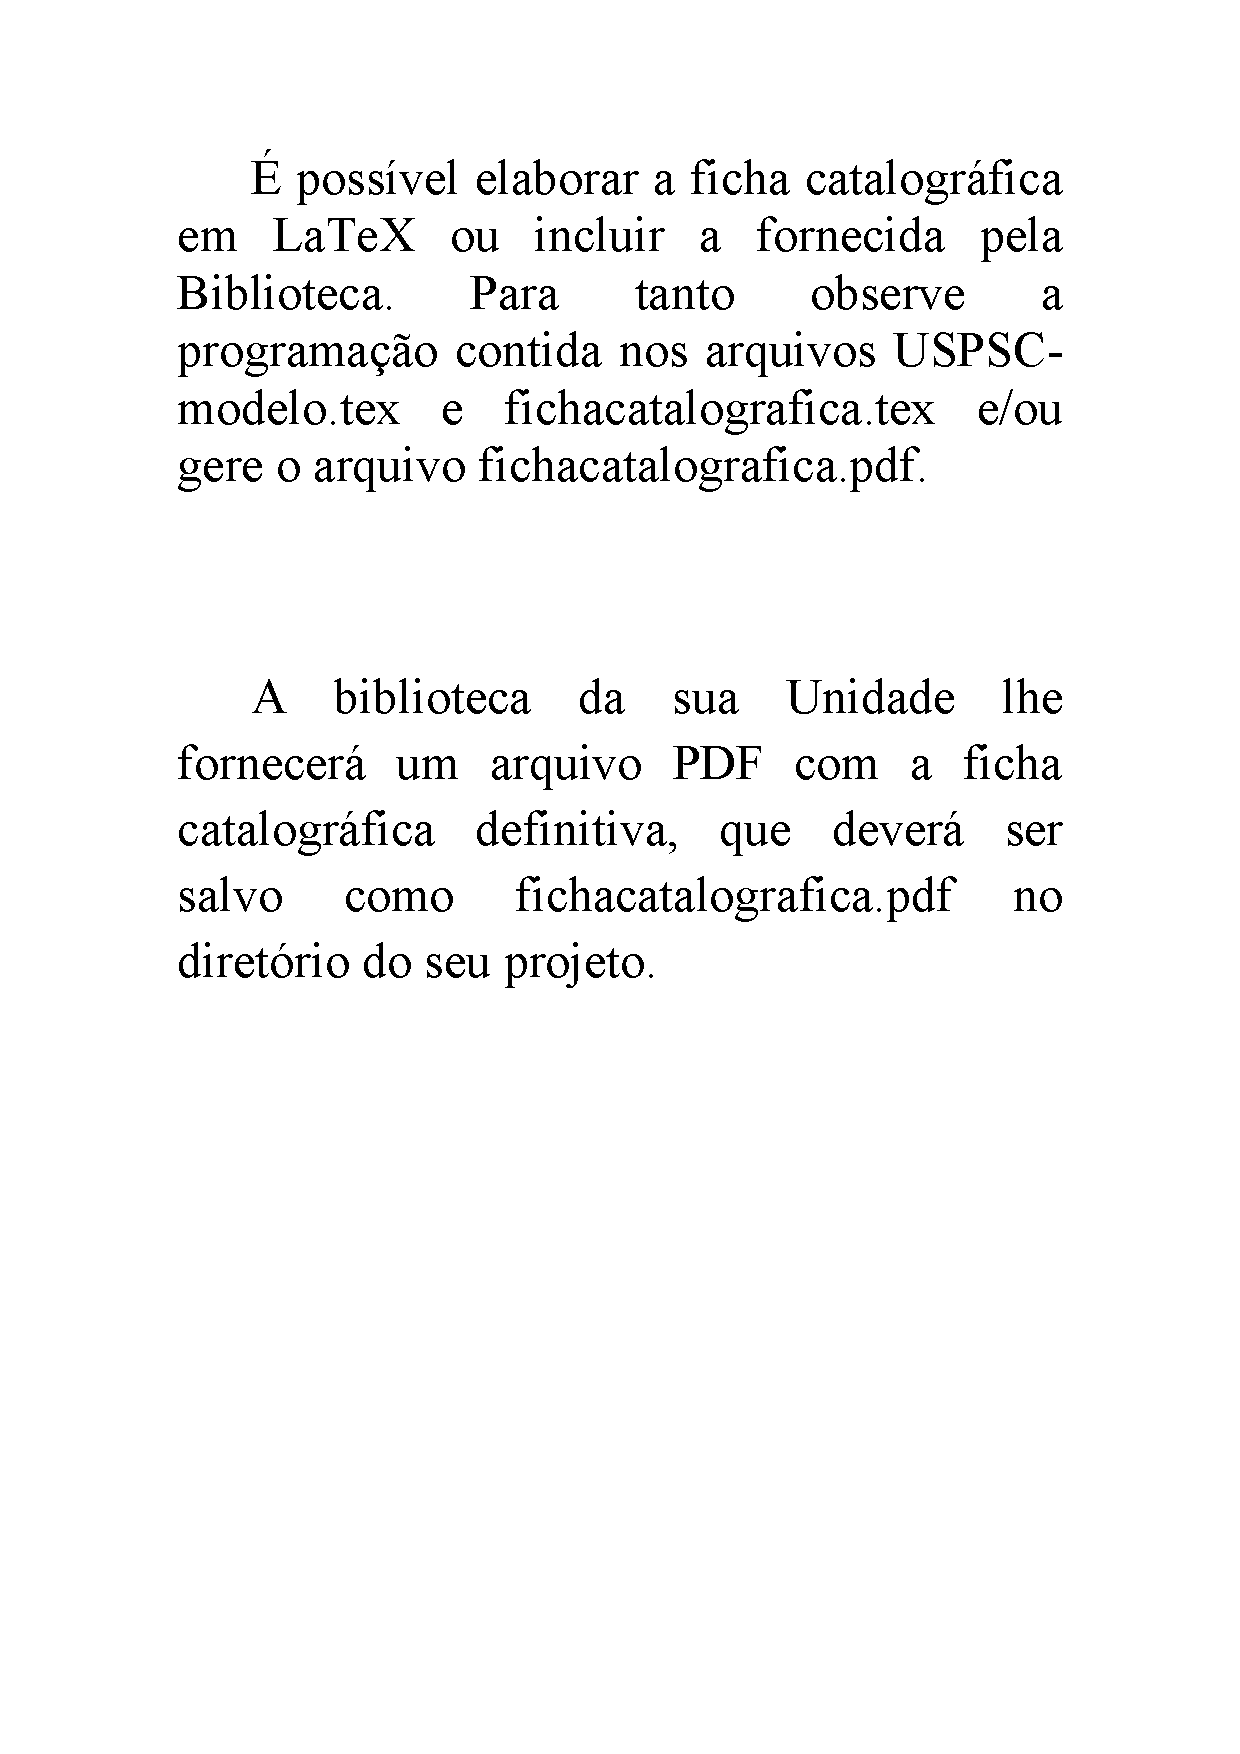
\includepdf{USPSC-TA-PreTextual/USPSC-fichacatalografica.pdf}

% Se você optar por elaborar a ficha catalográfica, deverá 
% incluir uma % antes da linha % antes
% do comando %% USPSC-fichacatalografica.tex
% ---
% Inserir a ficha bibliografica
% ---
% Isto é um exemplo de Ficha Catalográfica, ou ``Dados internacionais de
% catalogação-na-publicação''. Você pode utilizar este modelo como referência. 
% Porém, provavelmente a biblioteca da sua universidade lhe fornecerá um PDF
% com a ficha catalográfica definitiva após a defesa do trabalho. Quando estiver
% com o documento, salve-o como PDF no diretório do seu projeto e substitua todo
% o conteúdo de implementação deste arquivo pelo comando abaixo:
%
\begin{fichacatalografica}
	\hspace{-1.4cm}
	\imprimirnotaautorizacao \\ \\
	%\sffamily
	\vspace*{\fill}					% Posição vertical
\begin{center}					% Minipage Centralizado
  \imprimirnotabib \\
  \begin{table}[htb]
	\scriptsize
	\centering	
	\begin{tabular}{|p{0.9cm} p{8.7cm}|}
		\hline
	      & \\
		  &	  \imprimirautorficha     \\
		
		 \imprimircutter & 
							\hspace{0.4cm}\imprimirtitulo~  / ~\imprimirautor~ ;  ~\imprimirorientadorcorpoficha. -- 	\imprimirlocal, \imprimirdata.   \\
		
		  &  % Para incluir nota referente à versão corrigida no corpo da ficha,
			  % incluir % no início da linha acima e tirar a % do início da linha abaixo
			  %	\hspace{0.4cm} \imprimirtitulo~  / ~\imprimirautor~ ; ~\imprimirorientadorcorpoficha~- ~\imprimirnotafolharosto. -- \imprimirlocal, \imprimirdata.  \\
		
			\hspace{0.4cm}\pageref{LastPage} p. : il. (algumas color.) ; 30 cm.\\ 
		  & \\
		  & 
		    \hspace{0.4cm}\imprimirnotaficha ~--~ 
						  \imprimirunidademin, 
						  \imprimiruniversidademin, 
		                  \imprimirdata. \\ 
		  & \\                 
		   % Para incluir nota referente à versão corrigida em notas,
		    % incluir uma % no início da linha acima e	
		    % tirar a % do início da linha abaixo
		    % & \hspace{0.4cm}\imprimirnotafolharosto \\ 
		  & \\ 
		  & \hspace{0.4cm}1. LaTeX. 2. abnTeX. 3. Classe USPSC. 4. Editoração de texto. 5. Normalização da documentação. 6. Tese. 7. Dissertação. 8. Documentos (elaboração). 9. Documentos eletrônicos. I. \imprimirorientadorficha. 
		   II. Título. \\
	
		     %Se houver co-orientador, inclua % antes da linha (antes de II. Título.) 
		     %          e tire a % antes do comando abaixo 
		     %III. Título. \\   
		  \hline
	\end{tabular}
  \end{table}
\end{center}
\end{fichacatalografica}
% ---

 
% e retirar o % do comando abaixo
%%% USPSC-fichacatalografica.tex
% ---
% Inserir a ficha bibliografica
% ---
% Isto é um exemplo de Ficha Catalográfica, ou ``Dados internacionais de
% catalogação-na-publicação''. Você pode utilizar este modelo como referência. 
% Porém, provavelmente a biblioteca da sua universidade lhe fornecerá um PDF
% com a ficha catalográfica definitiva após a defesa do trabalho. Quando estiver
% com o documento, salve-o como PDF no diretório do seu projeto e substitua todo
% o conteúdo de implementação deste arquivo pelo comando abaixo:
%
\begin{fichacatalografica}
	\hspace{-1.4cm}
	\imprimirnotaautorizacao \\ \\
	%\sffamily
	\vspace*{\fill}					% Posição vertical
\begin{center}					% Minipage Centralizado
  \imprimirnotabib \\
  \begin{table}[htb]
	\scriptsize
	\centering	
	\begin{tabular}{|p{0.9cm} p{8.7cm}|}
		\hline
	      & \\
		  &	  \imprimirautorficha     \\
		
		 \imprimircutter & 
							\hspace{0.4cm}\imprimirtitulo~  / ~\imprimirautor~ ;  ~\imprimirorientadorcorpoficha. -- 	\imprimirlocal, \imprimirdata.   \\
		
		  &  % Para incluir nota referente à versão corrigida no corpo da ficha,
			  % incluir % no início da linha acima e tirar a % do início da linha abaixo
			  %	\hspace{0.4cm} \imprimirtitulo~  / ~\imprimirautor~ ; ~\imprimirorientadorcorpoficha~- ~\imprimirnotafolharosto. -- \imprimirlocal, \imprimirdata.  \\
		
			\hspace{0.4cm}\pageref{LastPage} p. : il. (algumas color.) ; 30 cm.\\ 
		  & \\
		  & 
		    \hspace{0.4cm}\imprimirnotaficha ~--~ 
						  \imprimirunidademin, 
						  \imprimiruniversidademin, 
		                  \imprimirdata. \\ 
		  & \\                 
		   % Para incluir nota referente à versão corrigida em notas,
		    % incluir uma % no início da linha acima e	
		    % tirar a % do início da linha abaixo
		    % & \hspace{0.4cm}\imprimirnotafolharosto \\ 
		  & \\ 
		  & \hspace{0.4cm}1. LaTeX. 2. abnTeX. 3. Classe USPSC. 4. Editoração de texto. 5. Normalização da documentação. 6. Tese. 7. Dissertação. 8. Documentos (elaboração). 9. Documentos eletrônicos. I. \imprimirorientadorficha. 
		   II. Título. \\
	
		     %Se houver co-orientador, inclua % antes da linha (antes de II. Título.) 
		     %          e tire a % antes do comando abaixo 
		     %III. Título. \\   
		  \hline
	\end{tabular}
  \end{table}
\end{center}
\end{fichacatalografica}
% ---


% As informações que compõem a ficha catalográfica estão 
% definidas no arquivo USPSC-pre-textual-UUUU.tex
% ---

% ---
% Folha de rosto adicional
% Para imprimir a folha de rosto adicional, exigida por algumas Unidades, a exemplo do ICMC,
% retire a % antes do comando abaixo

%\imprimirfolhaderostoadic

% ---
% ---
% Inserir errata
% ---

%%% USPSC-Errata.tex
\begin{errata}
	%\OnehalfSpacing 			
	A errata é um elemento opcional, que consiste de uma lista de erros da obra, precedidos pelas folhas e linhas onde eles ocorrem e seguidos pelas correções correspondentes. Deve ser inserida logo após a folha de rosto e conter a referência do trabalho para facilitar sua identificação, conforme a ABNT NBR 14724 \cite{nbr14724}.
	
	Modelo de Errata:
		
	\begin{flushleft} 
			\setlength{\absparsep}{0pt} % ajusta o espaçamento da referência	
			\SingleSpacing 
			\imprimirautorabr~ ~\textbf{\imprimirtituloresumo}.	\imprimirdata. \pageref{LastPage} p. 
			%Substitua p. por f. quando utilizar oneside em \documentclass
			%\pageref{LastPage} f.
			\imprimirtipotrabalho~-~\imprimirinstituicao, \imprimirlocal, \imprimirdata. 
 	\end{flushleft}
\vspace{\onelineskip}
\OnehalfSpacing 
\center
\textbf{ERRATA}
\vspace{\onelineskip}
\OnehalfSpacing 
\begin{table}[htb]
	\center
	\footnotesize
	\begin{tabular}{p{2cm} p{2cm} p{4cm} p{4cm} }
		\hline
		\textbf{Folha} & \textbf{Linha}  & \textbf{Onde se lê}  & \textbf{Leia-se}  \\
			\hline
			1 & 10 & auto-conclavo & autoconclavo\\
		\hline
	\end{tabular}
\end{table}
\end{errata}
% ---

% ---

% ---
% Inserir folha de aprovação
% ---

% A Folha de aprovação é um elemento obrigatório da NBR 4724/2011 (seção 4.2.1.3). 
% Após a defesa/aprovação do trabalho, gere o arquivo folhadeaprovacao.pdf da página assinada pela banca 
% e iclua o arquivo utilizando o comando abaixo:
%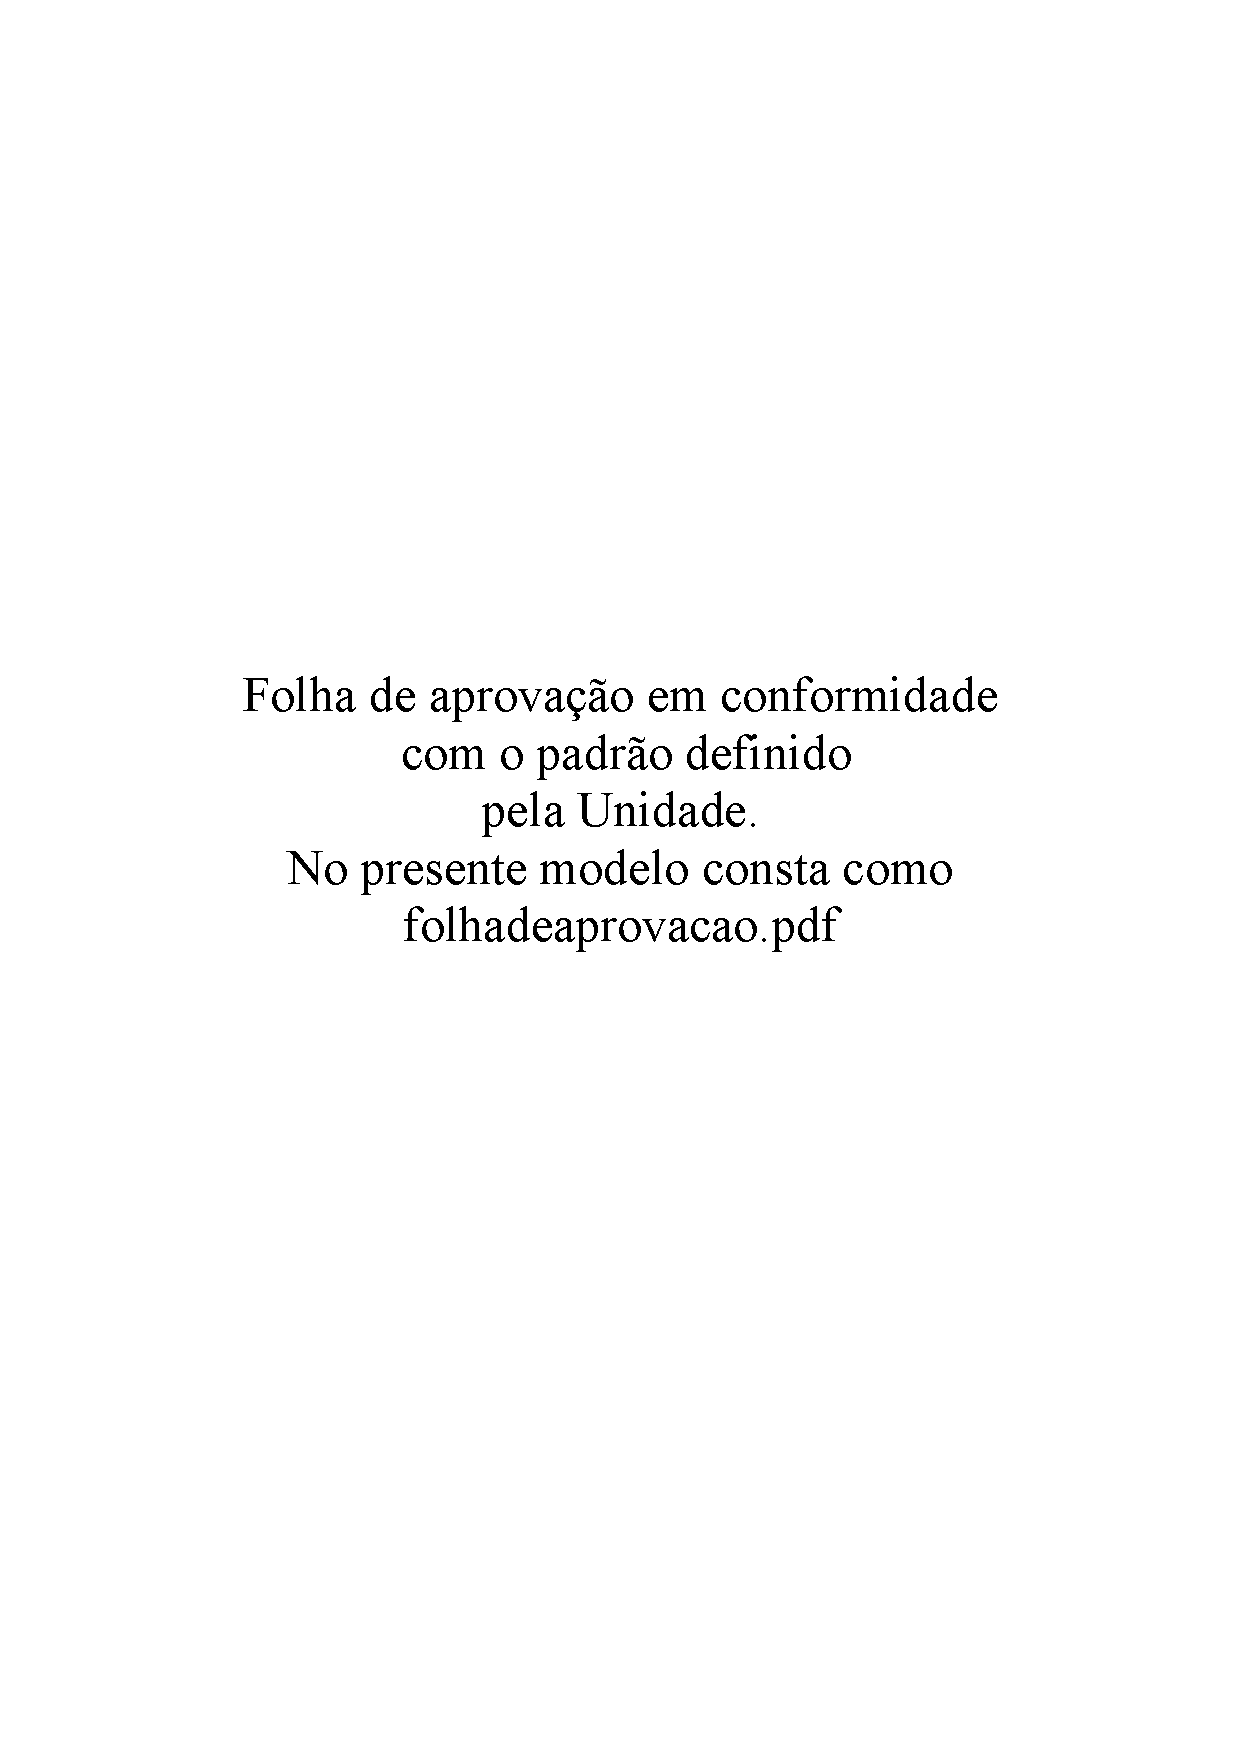
\includepdf{USPSC-TA-PreTextual/USPSC-folhadeaprovacao.pdf}
% Alternativa para a Folha de Aprovação:
% Se for a sua opção elaborar uma folha de aprovação, insira uma % antes do comando acima que inclui o arquivo folhadeaprovacao.pdf,
% tire o % do comando abaixo e altere o arquivo folhadeaprovacao.tex conforme suas necessidades
%\include{folhadeaprovacao}

\includepdf{USPSC-TA-PreTextual/USPSC-PaginaEmBranco.pdf}

% ---
% Dedicatória
% ---
%%% USPSC-Dedicatoria.tex
\begin{dedicatoria}
   \vspace*{\fill}
   \centering
   \noindent
   \textit{ Dedico esse trabalho aos meus pais, Marizete e Léo.} \vspace*{\fill}
\end{dedicatoria}
% ---
% ---

% ---
% Agradecimentos
% ---
%%% USPSC-Agradecimentos.tex
\begin{agradecimentos}
	Primeira frase do agradecimento ....
	
	Segunda frase ....
	
	Outras frases ....
	
	Última frase ....
	
\end{agradecimentos}
% ---
% ---

% ---
% Epígrafe
% ---
%%% USPSC-Epigrafe.tex
\begin{epigrafe}
    \vspace*{\fill}
	\begin{flushright}
		\textit{``O estudo, a busca da verdade e da beleza são domínios \\
		em que nos é consentido sermos crianças por toda a vida.''\\
		Albert Einstein}
	\end{flushright}
\end{epigrafe}
% ---
% ---

% A T E N Ç Ã O
% Se o idioma do texto for em inglês, o abstract deve preceder o resumo
% resumo em português
%
% Resumo
% ---
%% USPSC-Resumo.tex
\setlength{\absparsep}{18pt} % ajusta o espaçamento dos parágrafos do resumo		
\begin{resumo}
	\begin{flushleft} 
			\setlength{\absparsep}{0pt} % ajusta o espaçamento da referência	
			\SingleSpacing 
			\imprimirautorabr~~\textbf{\imprimirtituloresumo}.	\imprimirdata. \pageref{LastPage} p. 
			%Substitua p. por f. quando utilizar oneside em \documentclass
			%\pageref{LastPage} f.
			\imprimirtipotrabalho~-~\imprimirinstituicao, \imprimirlocal, \imprimirdata. 
 	\end{flushleft}
\OnehalfSpacing 			
	O presente trabalho teve como principal objetivo o desenvolvimento de uma ferramenta computacional robusta para a análise de problemas de interação fluido-estrutura, incorporando uma técnica de partição de domínios no escoamento fluido, de modo a capturar efeitos localizados.
Adota-se uma formulação estabilizada para análise dos escoamentos incompressíveis isotérmicos, permitindo aproximação de mesma ordem para as variáveis de velocidades e pressão, com uma integração temporal implicita realizada através do método $\alpha$-generalizado. A análise não-linear dinâmica da estrutura é modelada empregando-se uma abordagem do método dos elementos finitos baseada em posições aplicada a elementos de casca com integrador temporal de Newmark.
Nessa formulação, levam-se em conta os efeitos localizados no modelo do fluido através do uso de um modelo local mais refinado superposto a um modelo global com discretização mais grosseira. As discretizações utilizam aproximações baseadas na análise isogeométrica ou no método dos elementos finitos clássico. A união entre malha global e malha local é realizada através de uma formulação estabilizada do método de Arlequin, o qual efetua o cruzamento e colagem entre os modelos em uma zona de colagem através da utilização de campos de multiplicadores de Lagrange. Para garantir a estabilidade do campo de multiplicadores de Lagrange, e, ao mesmo tempo, fornecer maior flexibilidade a formulação, adiciona-se um termo consistente de estabilização, baseado no resíduo das equações governantes.
O acoplamento fluido-estrutura é do tipo particionado forte bloco-iterativo. Neste acoplamento, a malha local é adaptada à estrutura e deforma-se dinamicamente para acomodar a movimentação da estrutura, através de uma formulação ALE (Arbitrary Lagrangian–Eulerian), enquanto que a malha global permanece fixa. O  método de acoplamento proposto pode ser caracterizado como uma abordagem híbrida e  compartilha vantagens dos métodos de rastreamento de interface (malhas móveis) e de captura de interface (contornos imersos), visto que o fluido próximo à estrutura é adequadamente discretizado garantindo a captura de efeitos localizados, ao mesmo tempo em que a malha local, por ser menor, tolera maiores deformações, e em caso de necessidade de remalhamento, apenas essa malha precisa ser reconstruída. 
Os resultados obtidos nas simulações computacionais demonstraram a robustez e eficiência da formulação, evidenciando que trata-se de uma nova alternativa para análise de problemas de IFE com efeitos localizados.

 \textbf{Palavras-chave}: Interação Fluido-Estrutura.  Análise Isogeométrica. Método dos Elementos Finitos. Partição de domínios.
\end{resumo}
% ---

% Abstract
% ---
%% USPSC-Abstract.tex
%\autor{Silva, M. J.}
\begin{resumo}[Abstract]
 \begin{otherlanguage*}{english}
	\begin{flushleft} 
		\setlength{\absparsep}{0pt} % ajusta o espaçamento dos parágrafos do resumo		
 		\SingleSpacing  		\imprimirautorabr~~\textbf{\imprimirtitleabstract}.	\imprimirdata.  \pageref{LastPage} p. 
		%Substitua p. por f. quando utilizar oneside em \documentclass
		%\pageref{LastPage} f.
		\imprimirtipotrabalhoabs~-~\imprimirinstituicao, \imprimirlocal, 	\imprimirdata. 
 	\end{flushleft}
	\OnehalfSpacing 
   		The main objective of this work was the development of a robust computational tool for the analysis of fluid–structure interaction (FSI) problems, incorporating a domain partitioning technique in the fluid flow to capture localized effects.
   A stabilized formulation is adopted for the analysis of incompressible isothermal flows, allowing equal-order interpolation for velocity and pressure variables, with implicit time integration performed through the generalized-$\alpha$ method. The nonlinear dynamic analysis of the structure is modeled using a position-based finite element approach applied to shell elements, with time integration carried out by the Newmark method.
   In this formulation, localized effects in the fluid model are taken into account through the use of a refined local model superimposed on a coarser global model. The discretizations employ either isogeometric analysis or the classical finite element method. The coupling between the global and local meshes is achieved through a stabilized Arlequin method, which performs the coupling between models within an overlapping zone using Lagrange multiplier fields. To ensure the stability of the Lagrange multiplier field while providing greater flexibility to the formulation, a consistent stabilization term based on the residual of the governing equations is added.
   The fluid–structure coupling is strongly partitioned and block-iterative. In this coupling, the local mesh conforms to the structure and deforms dynamically to accommodate its motion through an Arbitrary Lagrangian–Eulerian (ALE) formulation, while the global mesh remains fixed. The proposed coupling method can be characterized as a hybrid approach, combining advantages of interface-tracking (moving-mesh) and interface-capturing (immersed-boundary) methods. The fluid near the structure is properly discretized to capture localized effects, while the smaller local mesh tolerates larger deformations; in case remeshing is required, only this local mesh needs to be reconstructed.
   The results obtained from the computational simulations demonstrated the robustness and efficiency of the formulation, showing that it provides a novel and effective alternative for the analysis of FSI problems with localized effects.

   \vspace{\onelineskip}
 
   \noindent 
   \textbf{Keywords}: Fluid-structure interaction. Isogeometric analysis. Finite Element Method. Domain Decomposition. 
 \end{otherlanguage*}
\end{resumo}

% ---

% ---
% inserir lista de figurass
% ---
\pdfbookmark[0]{\listfigurename}{lof}
\listoffigures*
\cleardoublepage
% ---

% ---
% inserir lista de tabelas
% ---
\pdfbookmark[0]{\listtablename}{lot}
\listoftables*
\cleardoublepage
% ---

% ---
% inserir lista de quadros
% ---
%\pdfbookmark[0]{\listofquadroname}{loq}
%\listofquadro*
%\cleardoublepage
% ---

% ---
% inserir lista de abreviaturas e siglas
% ---
%% USPSC-AbreviaturasSiglas.tex
\begin{siglas}
    \item[ABNT] Associação Brasileira de Normas Técnicas
    \item[abnTeX] ABsurdas Normas para TeX
	\item[IBGE] Instituto Brasileiro de Geografia e Estatística
	\item[LaTeX] Lamport TeX
	\item[USP] Universidade de São Paulo
	\item[USPSC] Campus USP de São Carlos
\end{siglas}

% ---

% ---
% inserir lista de símbolos
% ---
%% USPSC-Simbolos.tex
\begin{simbolos}
%  \item[$ \velocity $] Vetor de velocidade com componentes $u_1$, $u_2$ e $u_3$
  %\nomenclature[B,02]{$\time$}{Instante de tempo arbitrário;}
  %\nomenclature[B,03]{$\density$}{Massa específica do fluido;}
  %\nomenclature[B,04]{$dV$}{Volume de controle infinitesimal;}
  %\nomenclature[B,05]{$dA_i$}{Área referente à face ortogonal ao eixo $y_i$ do volume de controle infinitesimal;}
  %\nomenclature[B,06]{$dy_i$}{Dimensão do volume de controle infinitesimal na direção $y_i$;}
  %\nomenclature[B,07]{$\mathbf{F}$}{Vetor da resultante das forças externas atuando em um volume de controle infinitesimal, com componentes $F_1$, $F_2$ e $F_3$}
  %\nomenclature[B,08]{$\stressTensor$}{Tensor de tensões de Cauchy de componentes $\sigma_ij$ com $i,j = 1,2,3$;}
  %\nomenclature[B,09]{$\mathbf{b}$}{Vetor forças de campo por unidade de volume com componentes $b_1$, $b_2$ e $b_3$;}
  %\nomenclature[B,10]{$\mathbf{q}$}{Vetor resultante das forças externas por unidade de volume com componentes $q_1$, $q_2$ e $q_3$;}
  %\nomenclature[B,11]{$\sbodyforce$}{Vetor que representa a força de campo por unidade de massa, com componentes $f_1$, $f_2$ e $f_3$;}
  %\nomenclature[B,12]{$\press$}{Campo de pressões de um escoamento;}
  %\nomenclature[B,13]{$\viscosity$}{Viscosidade dinâmica do fluido;}
  %\nomenclature[B,14]{$\straintensor(\bullet)$}{Tensor taxa de deformação infinitesimal;}
  %\nomenclature[B,15]{$\domain$}{Domínio espacial ou domínio atual do escoamento do fluido;}
  %\nomenclature[B,16]{$\nsd$}{Dimensão espacial;}
  %\nomenclature[B,17]{$\boundary$}{Contorno do domínio espacial que define o escoamento do fluido;}
  %\nomenclature[B,18]{$\boundaryD$}{Porção do contorno com condições de contorno de Dirichlet;}
  %\nomenclature[B,19]{$\boundaryN$}{Porção do contorno com condições de contorno de Neumann;}
  %\nomenclature[B,20]{$\totalTime$}{Intervalo de tempo total da análise;}
  %\nomenclature[B,21]{$\velocityD$}{Vetor de velocidades prescritas;}
  %\nomenclature[B,22]{$\surfaceLoad$}{Forças de superfície prescritas;}
  %\nomenclature[B,23]{$\snormal$}{Vetor normal ao contorno do domínio computacional;}
  %\nomenclature[B,24]{$\domainMat$}{Domínio inicial ou material do escoamento do fluido;}
  %\nomenclature[B,25]{$\posMat$}{Vetor das coordenadas dos pontos materiais de um ponto arbitrário;}
  %\nomenclature[B,26]{$\pos$}{Vetor das coordenadas atuais de um ponto arbitrário;}
  %\nomenclature[B,27]{$\domainRef$}{Domínio de referência do escoamento do fluido;}
  %\nomenclature[B,28]{$\posAle$}{Vetor das coordenadas de referência de um ponto arbitrário;}
  %\nomenclature[B,29]{$\fmapAI(\posMat,t)$}{Função mudança de configuração do domínio material para o domínio espacial;}
  %\nomenclature[B,30]{$\fmapAR(\posALE,t)$}{Função mudança de configuração do domínio de referência para o domínio espacial;}
  %\nomenclature[B,31]{$\fmapRI(\posMat,t)$}{Função mudança de configuração do domínio material para o domínio de referência;}	
  %\nomenclature[B,32]{$\velocityALE$}{Velocidade dos pontos de referência;}
  %\nomenclature[B,33]{$\FmapAI$}{Matriz jacobiana da função de mapeamento $\fmapAI(\posMat,t)$;}
  %\nomenclature[B,34]{$\FmapAR$}{Matriz jacobiana da função de mapeamento $\fmapAR(\posALE,t)$;}
  %\nomenclature[B,35]{$\FmapRI$}{Matriz jacobiana da função de mapeamento $\fmapRI(\posMat,t)$;}
  %\nomenclature[B,36]{$g,g^{*},g^{**}$}{Grandeza física escalar na configuração espacial, de referência e material respectivamente;}
  %\nomenclature[B,37]{$\usolution$}{Espaço vetorial das funções aproximadoras do campo de velocidades;}
  %\nomenclature[B,38]{$\psolution$}{Espaço vetorial das funções aproximadoras do campo de pressões;}
  %\nomenclature[B,39]{$\uweighting$}{Espaço vetorial das funções ponderadoras do campo de velocidades;}
  %\nomenclature[B,40]{$\pweighting$}{Espaço vetorial das funções ponderadoras do campo de pressões;}
  %\nomenclature[B,41]{$\utest$}{Função ponderadora pertencente ao espaço $\uweighting$;}
  %\nomenclature[B,42]{$\ptest$}{Função ponderadora pertencente ao espaço $\pweighting$;}
  %\nomenclature[B,43]{$(\bullet)^h$}{O superscrito $h$ indica, em todos os casos, a discretização em elementos finitos da variável;}
  %\nomenclature[B,44]{$\domainE$}{Domínio computacional de um elemento finito;}
  %\nomenclature[B,45]{$\nel$}{Número de subdomínios do domínio discreto;}
  %\nomenclature[B,46]{$\nnos$}{Número de nós ou pontos de controle do domínio discreto;}
  %\nomenclature[B,47]{$\boundary^{b}$}{Domínio computacional de um elemento finito no contorno;}
  %\nomenclature[B,48]{$\neb$}{Número de subdomínios do domínio discreto no contorno;}
  %\nomenclature[B,49]{$\shapef$}{Função de forma da discretização do domínio;}
  %\nomenclature[B,50]{$(\bullet)_A$}{O subscrito $A$ indica, em todos os casos, que se trata da variável respectiva ao nó $A$ da malha de elementos finitos;}
  %\nomenclature[B,51]{$\SUPG$}{Parâmetro de estabilização do método \textit{Streamline-Upwind/Petrov-Galerkin} (SUPG);}
  %\nomenclature[B,52]{$\PSPG$}{Parâmetro de estabilização do método \textit{Pressure-Stabilizing/Petrov-Galerkin} (PSPG);}
  %\nomenclature[B,53]{$\LSIC$}{Parâmetro de estabilização do método \textit{Least-Squares on the Incompressibility Constraint} (LSIC);}
  %\nomenclature[B,54]{$\resMom$}{Resíduo da equação da quantidade de movimento;}
  %\nomenclature[B,55]{$\resPre$}{Resíduo da equação da continuidade;}
  %\nomenclature[B,56]{$\NNSM$}{Resíduo do vetor semidiscreto da equação da quantidade de movimento;}
  %\nomenclature[B,57]{$\NNSC$}{Resíduo do vetor semidiscreto da equação da continuidade;}
  %\nomenclature[B,58]{$\Acceleration$}{Vetor nodal dos graus de liberdade respectivo a aceleração;}
  %\nomenclature[B,59]{$\Velocity$}{Vetor nodal dos graus de liberdade respectivo a velocidade;}
  %\nomenclature[B,60]{$\Press$}{Vetor nodal dos graus de liberdade respectivo a pressão;}
  %\nomenclature[B,61]{$\matrixQ$}{Matriz Jacobiana do elemento;}
  %\nomenclature[B,62]{$\coordAdimen$}{Vetor das coordenadas paramétricas adimensionais do elemento com componentes $\xi$, $\eta$ $\zeta$;}
  %\nomenclature[B,63]{$\matrixD$}{Matriz que realiza mudança de escala em $\matrixQ$ para levar em conta o grau polinomial das funções de forma;}
  %\nomenclature[B,64]{$\matrixQhat$}{Matriz jacobiana escalonada;}
  %\nomenclature[B,65]{$\RGN$}{Comprimento direcional do elemento finito;}
  %\nomenclature[B,66]{$\rRGN$}{Vetor unitário no sentido do gradiente da intensidade da velocidade;}
  %\nomenclature[B,67]{$\matrixG$}{Tensor métrico do elemento;}
  %\nomenclature[B,68]{$h_{min}$}{Mínimo comprimento de escala do elemento finito;}
  %\nomenclature[B,69]{$h_{max}$}{Máximo comprimento de escala do elemento finito;}
  %\nomenclature[B,70]{$\lambda_{min},\lambda_{max}$}{mínimo e máximo autovalor da matriz $\matrixG$;}
  %\nomenclature[B,71]{$\SUGNi,\SUGNii,\SUGNiii$}{Parâmetros da estabilização SUPG/PSPG/LSIC correspondentes aos termos convectivos, inerciais e viscosos, respectivamente;}
  %\nomenclature[B,72]{$\rRGN_{reg}$}{Vetor unitário no sentido do gradiente da intensidade da velocidade do fluido modificado de maneira a evitar problemas numéricos devido divisão por zero;}
  %\nomenclature[B,73]{$\varepsilon$}{Constante pequena utilizada no cálculo de $\rRGN_{reg}$;}
  %\nomenclature[B,74]{$t_{n}$}{é o tempo atual, ou seja, o instante n-ésimo no qual a solução foi calculada.;}
  %\nomenclature[B,75]{$t_{n+1}$}{é o próximo instante de tempo, ou seja, o instante $n+1$ no qual solução será calculada;}
  %\nomenclature[B,76]{$\alpham, \alphaf, \gamma$}{Parâmetros reais do esquema de integração temporal $\alpha$-generalizado;}
  %\nomenclature[B,77]{$\specRadius$}{Raio espectral da matriz de amplificação;}
  %\nomenclature[B,78]{$\Reynolds$}{Número de Reynolds;}
  %\nomenclature[B,79]{$\velocinfty$}{Velocidade de referência;}
  %\nomenclature[B,80]{$L$}{Comprimento característico/de referência do escoamento;}
  %\nomenclature[B,81]{$\kviscosity$}{Viscosidade cinemática do fluido;}
  %\nomenclature[B,82]{$F_L, F_D$}{Forças de sustentação e arrasto, respectivamente;}
  %\nomenclature[B,83]{$C_L, C_D$}{Coeficiente de sustentação e arrasto, respectivamente;}
  %\nomenclature[B,84]{$\Strouhal$}{Número de Strouhal;}
  %\nomenclature[B,85]{$f_v$}{Frequência de desprendimento dos vórtices;}
  %\nomenclature[C,01]{$p$}{Grau das funções base na direção paramétrica $\xsi$;}
  %\nomenclature[C,02]{$\xsi$}{Vetor de \textit{knots} na direção paramétrica $\xsi$;}
  %\nomenclature[C,03]{$\xsi$}{Uma das direções paramémtricas nas quais as funções base são definidas;}
  %\nomenclature[C,04]{$n$}{Número de funções base na direção paramétrica $\xsi$ ;}
  %\nomenclature[C,05]{$N$}{Função base \textit {B-Spline} na direção paramétrica $\xsi$ ;}
  %\nomenclature[C,06]{$\CP$}{Pontos de controle que descrevem a geometria \textit{B-Spline} ou NURBS;}
  %\nomenclature[C,07]{$\mathbf{C}$}{Curva \textit {B-Spline} ou NURBS;}
  %\nomenclature[C,08]{$m$}{Grau das funções base na direção paramétrica $\eta$;}
  %\nomenclature[C,09]{$\mathcal{H}$}{Vetor de \textit{knots} na direção paramétrica $\eta$;}
  %\nomenclature[C,10]{$q$}{Número de funções base na direção paramétrica $\eta$ ;}
  %\nomenclature[C,11]{$\eta$}{Uma das direções paramémtricas nas quais as funções base são definidas;}
  %\nomenclature[C,12]{$M$}{Função base \textit {B-Spline} na direção paramétrica $\eta$ ;}
  %\nomenclature[C,13]{$\mathbf{S}$}{Superfície \textit {B-Spline} ou NURBS;}
  %\nomenclature[C,14]{$\hat{N}$}{Função \textit {B-Spline} fruto do produto tensorial entre funções base descritas em um espaço paramétrico qualquer;}
  %\nomenclature[C,15]{$L$}{Função base \textit {B-Spline} na direção paramétrica $\zeta$ ;}
  %\nomenclature[C,16]{$r$}{Grau das funções base na direção paramétrica $\zeta$;}
  %\nomenclature[C,17]{$\mathcal{Z}$}{Vetor de \textit{knots} na direção paramétrica $\zeta$;}
  %\nomenclature[C,18]{$\zeta$}{Uma das direções paramémtricas nas quais as funções base são definidas;}
  %\nomenclature[C,19]{$l$}{Número de funções base na direção paramétrica $\zeta$ ;}
  %\nomenclature[C,20]{$\mathbf{T}$}{Sólido \textit {B-Spline} ou NURBS;}
  %\nomenclature[C,21]{$\mathbf{C}^{w}$}{Curva \textit{B-Spline} no $\realspace^{d+1}$ cuja projeção transformativa gera uma curva \mathbf{C} no $\realspace^{d}$;}
  %\nomenclature[C,22]{$R$}{Função base NURBS;}
  %\nomenclature[C,23]{$w$}{Peso respectivo a um ponto de controle;}
  %\nomenclature[C,24]{$\mathbf{\hat{\xsi}}$}{Coordenadas do espaço parental, no qual realiza-se a integração numérica;}
  %\nomenclature[C,25]{$\hat{\xsi}$}{Uma das direções do espaço parental;}
  %\nomenclature[C,26]{$\hat{\eta}$}{Uma das direções do espaço parental;}
  %\nomenclature[C,27]{$\hat{\zeta}$}{Uma das direções do espaço parental;}
  %\nomenclature[C,28]{$\tilde{\Omega^{e}}$}{Domínio de uma célula no espaço paramétrico;}
  %\nomenclature[C,29]{$\hat{\Omega^{e}}$}{Domínio de um uma célula o no espaço parental;}
  %\nomenclature[C,30]{$h$}{Dimensão na direção $y$ da entrada do perfil parabólico no problema do escoamento sobre canal com degrau;}
  %\nomenclature[C,31]{$s$}{Dimensão  na direção $y$ do degrau que compõe o problema do escoamento sobre canal com degrau;}
  %\nomenclature[C,32]{$x_{e}$}{Dimensão na direção $x$  do degrau que compõe o problema do escoamento sobre canal com degrau;}
  %\nomenclature[C,33]{$x_{f}$}{Dimensão na direção $x$  do \textit{patch} $P1$ do problema do escoamento sobre canal com degrau;}
  %\nomenclature[C,34]{$x_{t}$}{Dimensão do canal após o degrau na direção $x$ do problema do escoamento sobre canal com degrau;}
  %\nomenclature[C,35]{$V_{max}$}{Velocidade máxima do perfil parabólico na entrada do problema do escoamento sobre canal com degrau;}
  %\nomenclature[C,36]{$x_{r}$}{Dimensão do vórtice primário que se forma no problema de escoamento sobre canal com degrau;}
  %\nomenclature[C,37]{$P_{i}$}{Patch de número $i$;}
%  	\nomenclature[D,01]{$\Omega_{x}$}{Domínio inicial de um sólido deformável;}
%  \nomenclature[D,02]{$\lPosition$}{Coordenadas ou posições materiais do domínio inicial;}
%  \nomenclature[D,03]{$\Omega_{y}$}{Domínio atual de um sólido deformável;}
%  \nomenclature[D,04]{$\ePosition$}{Coordenadas ou posições espaciais do domínio atual;}
%  \nomenclature[D,05]{$\deformation$}{Função mudança de configuração para um descrição Lagrangiana;}
%  \nomenclature[D,06]{$\greenStrain$}{Tensor de deformações de Green-Lagrange;}
%  \nomenclature[D,07]{$\cauchyStretch$}{Tensor de alongamento à direita de Cauchy-Green;}
%  \nomenclature[D,08]{$\gradDeformation$}{Grandiente da função mudança de configuração;}
%  \nomenclature[D,09]{$\mathbf{u}$}{Vetor qualquer definido na configuração inicial;}
%  \nomenclature[D,10]{$\mathbf{v}$}{Vetor qualquer definido na configuração atual;}
%  \nomenclature[D,11]{$dV_{0}$}{Infinitésimo de volume definido na configuração inicial;}
%  \nomenclature[D,12]{$dV$}{Infinitésimo de81 volume definido na configuração atual;}
%  \nomenclature[D,13]{$\mathbf{dx}^{i}$}{Vetor que define o lado $i$ de um infinitésimo de volume na configuração inicial, com $i = 1,2,3$;}
%  \nomenclature[D,14]{$dx_{j}^{i}$}{Componente do vetor $mathbf{dx}^{i}$ na direção do eixo $x_{j}$;}
%  \nomenclature[D,15]{$\mathbf{dy}^{i}$}{Vetor que define o lado $i$ de um infinitésimo de volume na configuração atual, com $i = 1,2,3$;}
%  \nomenclature[D,16]{$dy_{j}^{i}$}{Componente do vetor $mathbf{dy}^{i}$ na direção do eixo $y_{j}$;}
%  \nomenclature[D,17]{J}{Jacobiano da transformação, definido como $det(\gradDeformation)$};
%  \nomenclature[D,18]{$\mathbf{dA}_{0}$}{Vetor de área da seção transversal de um volume na configuração inicial;}
%  \nomenclature[D,19]{$\mathbf{dA}$}{Vetor de área da seção transversal de um volume na configuração atual;}
%  \nomenclature[D,20]{$\mathbf{N}$}{Vetor normal a uma superfície na configuração inicial;}
%  \nomenclature[D,21]{$\mathbf{n}$}{Vetor normal a uma superfície na configuração atual;}
%  \nomenclature[D,22]{${dA}_{0}$}{Área da seção transversal de um volume na configuração inicial;}
%  \nomenclature[D,23]{${dA}$}{Área da seção transversal de um volume na configuração atual;}
%  \nomenclature[D,24]{$\mathbf{B}$}{Tensor definido como $\mathbf{B} = \gradDeformation^{-t}$;}
%  \nomenclature[D,25]{$\extEnergy$}{Energia potencial das forças externas;}
%  \nomenclature[D,26]{$\intEnergy$}{Energia de deformação;}
%  \nomenclature[D,27]{$\kinEnergy$}{Energia cinética;}
%  \nomenclature[D,28]{$\totalEnergy$}{Energia total mecânica;}
%  \nomenclature[D,29]{$\delta(\bullet)$}{Variação aplicada a variável $(\bullet)$;}
%  \nomenclature[D,30]{$\ebodyLoad$}{Forças de corpo na configuração atual;}
%  \nomenclature[D,31]{$\tractionLoad$}{Forças de superfície na configuração atual;}
%  \nomenclature[D,32]{$\stressTensor$}{Tensor de tensões de Cauchy;}
%  \nomenclature[D,33]{$\rho$}{Massa específica do sólido;}
%  \nomenclature[D,34]{$\solidAccel$}{Aceleração do sólido;}
%  \nomenclature[D,35]{$\strainratetensor$}{Tensor de deformação linear de engenharia;}
%  \nomenclature[D,36]{$M$}{Massa de um corpo;}
%  \nomenclature[D,37]{$t$}{Instante de tempo qualquer da análise;}
%  \nomenclature[D,38]{$\rho_{0}$}{Massa específica do corpo na configuração inicial;}
%  \nomenclature[D,39]{$\ebodyLoad^{0}$}{Forças de corpo na configuração inicial;}
%  \nomenclature[D,40]{$\mathbf{P}$}{Tensor de tensões de Piola Kirchhoff;}
%  \nomenclature[D,41]{$\tractionLoad^{0}$}{Forças de superfície na configuração inicial;}
%  \nomenclature[D,42]{$\piolaStress$}{Segundo tensor de tensões de Piola Kirchhoff;}
%  \nomenclature[D,43]{$u_{e}$} {Expressão generalizada da energia de deformação;}
%  \nomenclature[D,44]{$\constitutiveTensor$}{Tensor constitutivo elástico isotrópico;}
%  \nomenclature[D,45]{$\bulkModulus$}{Módulo volumétrico;}
%  \nomenclature[D,46]{$\shearModulus$}{Módulo de cisalhamento;}
%  \nomenclature[D,47]{$\elasticModulus$ }{Módulo de elasticidade;}
%  \nomenclature[D,48]{$\poisonsRatio$}{Coeficiente de Poisson;}
%  \nomenclature[D,49]{$\deformation^{m0}$}{Função mudança de configuração da superfície média de uma casca que mapeia o domínio paramétrico para o domínio inicial;}
%  \nomenclature[D,50]{$\lPosition^{m}$}{Posições da superfície média de uma casca na configuração inicial;}
%  \nomenclature[D,51]{$\bm{\xi}$}{Coordenadas adimensionais que definem o espaço paramétrico}
%  \nomenclature[D,52]{$\mathbf{X}$}{Posições discretas nodais de um elemento de casca na configuração inicial;}
%  \nomenclature[D,53]{$N$}{Funções de forma}
%  \nomenclature[D,54]{$\deformation^{m1}$}{Função mudança de configuração da superfície média de uma casca que mapeia o domínio paramétrico para o domínio atual;}
%  \nomenclature[D,55]{$\ePosition^{m}$}{Posições da superfície média de uma casca na configuração atual;}
%  \nomenclature[D,56]{$\SolidPos$}{Posições discretas nodais de um elemento de casca na configuração atual;}
%  \nomenclature[D,57]{$\mathbf{v}^{0}$}{Vetor posição definido a partir da superfície média da casca em sua configuração inicial;}
%  \nomenclature[D,58]{$\mathbf{v}^{1}$}{Vetor posição definido a partir da superfície média da casca em sua configuração atual;}
%  \nomenclature[D,59]{$h_{0}$}{Espessura média inicial de um elemento de casca;}
%  \nomenclature[D,60]{$\mathbf{V}^{0}$}{Vetor posição discreto nodal na configuração inicial;}
%  \nomenclature[D,61]{$\mathbf{V}^{1}$}{Vetor posição discreto nodal na configuração atual;}
%  \nomenclature[D,62]{$\alpha$}{Taxa linear de variação da espessura de um elemento de casca;}
%  \nomenclature[D,63]{$\Lambda$}{Taxa linear discreta nodal da variação da espessura de um elemento de casca;}
%  \nomenclature[D,64]{$\deformation^{0}$}{Função mudança de configuração de uma casca que mapeia o domínio paramétrico para o domínio inicial;}
%  \nomenclature[D,65]{$\deformation^{1}$}{Função mudança de configuração de uma casca que mapeia o domínio paramétrico para o domínio atual;}
%  \nomenclature[D,66]{$\mathbf{F}$}{Vetor de forças nodais aplicadas na configuração inicial;}
%  \nomenclature[D,67]{$\gradDeformation^{1}$}{Gradiente da função mudança de configuração $\deformation^{1}$;}
%  \nomenclature[D,68]{$\gradDeformation^{0}$}{Gradiente da função mudança de configuração $\deformation^{0}$;}
%  \nomenclature[D,69]{$\mathbf{B}^{0}$}{Vetor discreto nodal que define as forças de corpo na configuração inicial;}
%  \nomenclature[D,70]{$\mathbf{Q}^{0}$}{Vetor discreto nodal que define as forças de superfície na configuração inicial;}
%  \nomenclature[D,71]{$\mathbf{\ddot{Y}}$}{Vetor discreto nodal que define a aceleração;}
%  \nomenclature[D,72]{$\concLoad^{ext}$}{Vetor discreto nodal que define as forças externas atuantes em um sólido;}
%  \nomenclature[D,73]{$\solidMass$}{Matriz de massa de um elemento;}
%  \nomenclature[D,74]{$\concLoad^{int}$}{Vetor discreto nodal que define as forças internas atuantes em um sólido;}
%  \nomenclature[D,75]{$\solidDamping$}{Matriz de amortecimento de um elemento;}
%  \nomenclature[D,76]{$\SolidVel_{}$}{Vetor discreto nodal que define a velocidade;}
%  \nomenclature[D,77]{$t_{n+1}$}{Tempo discreto no instante atual;} 
%  \nomenclature[D,78]{$t_{n}$}{Tempo discreto no instante anterior;} 
%  \nomenclature[D,79]{$\Delta t$}{Intervalo de tempo da discretização temporal;}
%  \nomenclature[D,80]{$\beta$}{Parâmetro da aproximação temporal de Newmark;}
%  \nomenclature[D,81]{$\gamma$}{Parâmetro da aproximação temporal de Newmark;}
%  \nomenclature[D,82]{$\mathbf{Q}_n$ e $\mathbf{R}_n$}{Termos da aproximação de Newmark que relacionam velocidade, aceleração e posições em um instante de tempo anterior;}
%  \nomenclature[D,83]{$\NNSS$}{Vetor discreto que representa o resíduo da equação de equilíbrio discretizada no espaço e tempo;}
%	\nomenclature[F,01]{$(\bullet)_{0}, (\bullet)_{1}$}{Subíndices que designam o modelo Global e o modelo Local respectivamente;}
%	\nomenclature[F,02]{$\overlappingZone$}{Zona de superposição;}
%	\nomenclature[F,03]{$\gluingZone$}{Zona de colagem;}
%	\nomenclature[F,04]{$\freeZone$}{Zona livre;}
%	\nomenclature[F,05]{$\lagrangeMultiplier$}{Campo de multiplicadores de Lagrange;}
%	\nomenclature[F,06]{$k_{0},k_{1}$}{Constantes dos operadores de acoplamento;}
%	\nomenclature[F,07]{$L^{2}$}{Operador de acoplamento de ordem 0;}
%	\nomenclature[F,08]{$H^{1}$}{Operador de acoplamento de ordem 1;}
%	\nomenclature[F,09]{$\arlequinWF$}{Função ponderadora;}
%	\nomenclature[F,10]{$k_{a}$}{Constante arbitrária do método de Arlequin;}
%	\nomenclature[F,11]{$\lagSolution$}{Espaço vetorial das funções aproximadoras do campo de multiplicadores de Lagrange;}
%	\nomenclature[F,12]{$\lagTest$}{Espaço vetorial das funções ponderadoras do campo de multiplicadores de Lagrange;}
%	\nomenclature[F,13]{$\lagrangeMultiplierWFh$}{Função ponderadora pertencente ao espaço $\lagTest$;}
%	\nomenclature[F,14]{$\chi$}{Função lógica para determinação do pertencimento de um ponto à $\gluingZone$;}
%	\nomenclature[F,15]{$\tauArlequin$}{Parâmetro de estabilização da técnica RBSAM;}
%	\nomenclature[F,16]{$\mathbf{K}_{i}$}{Matriz que representa os termos provenientes das matrizes referentes as equações da quantidade de movimento e da continuidade para o modelo $i$;}
%	\nomenclature[F,17]{$\mathbf{\hat{L}}_{i}$}{Matriz que representa os termos oriundos do acoplamento do modelo $i$;;}
%	\nomenclature[F,18]{$\mathbf{L}_{i}^{T}$}{Matriz procedente dos termos da equação de restrição e de componentes da estabilização RBSAM do modelo $i$;}
%	\nomenclature[F,19]{$\mathbf{E}$}{Matriz com termos oriundos da estabilização RBSAM;}
%	\nomenclature[F,20]{$\mathbf{\bar{U}}_{i}$}{Representa os vetores nodais dos graus de liberdade respectivos a velocidade e pressão do modelo $i$;}
%	\nomenclature[F,21]{$\LagrangeMultiplier$}{Representa os graus de liberdade respectivos aos multiplicadores de Lagrange;}
%	\nomenclature[F,22]{$\mathbf{F}_{i}$}{Representam os vetores provenientes das equações da quantidade de movimento e da continuidade do modelo $i$;}
%	\nomenclature[F,23]{$\mathbf{F}_{\LagrangeMultiplier}$}{Representa os termos vetoriais advindos da estabilização RBSAM;}
%	\nomenclature[F,24]{$\NNSL$}{Resíduo da versão semidiscreta da equação de restrição}
%	\nomenclature[F,25]{$\tau_{A},\tau_{A}^{0},\tau_{A}^{1}}{Parâmetros auxiliares para a determinação de $\tauArlequin$;}
%	\nomenclature[F,26]{$\tau_{B},\tau_{B}^{0},\tau_{B}^{1}}{Parâmetros auxiliares para a determinação de $\tauArlequin$;}
%	\nomenclature[F,27]{$\tau_{C},\tau_{C}^{0},\tau_{C}^{1}}{Parâmetros auxiliares para a determinação de $\tauArlequin$;}
%	\nomenclature[F,28]{$\tau_{D},\tau_{D}^{0},\tau_{D}^{1}}{Parâmetros auxiliares para a determinação de $\tauArlequin$;}
%	\nomenclature[F,29]{$\tau_{E},\tau_{E}^{0},\tau_{E}^{1}}{Parâmetros auxiliares para a determinação de $\tauArlequin$;}
%	\nomenclature[F,30]{$\tau_{E},\tau_{E}^{0},\tau_{E}^{1}}{Parâmetros auxiliares para a determinação de $\tauArlequin$;}	
%	\nomenclature[F,31]{$\mathbf{M}_{\lambda},\mathbf{t}, \mathbf{j}, \mathbf{k}, \mathbf{p}, \mathbf{\boundary}$}{Vetores elementares da formulação usadas na definição de $\tauArlequin$, relativo aos termos de restrição, convectivos, inerciais, viscosos, pressão e de acoplamento respectivamente;}
%	\nomenclature[F,32]{$C$}{Corda: distância entre o bordo ataque e de fuga do aerofólio;}	
%	\nomenclature[F,33]{$\theta, \theta_{max}, \theta_{min}$}{Ângulo de ataque; Ângulo de ataque máximo; Ângulo de ataque mínimo;}	
%	\nomenclature[F,34]{$f_{o}$}{Frequência de oscilação;}
%	\nomenclature[G,01]{$\domainFSI$}{Domínio computacional de problemas de Interação Fluido Estrutura;}
%	\nomenclature[G,02]{$(\bullet)_{F}, (\bullet)_{E}, (\bullet)_{M}$}{Subíndices que designam fluido, estrutura e malha respectivamente;}
%	\nomenclature[G,03]{$\boundaryFSI$}{Contorno que define a interface fluido-estrutura;}
%	\nomenclature[G,04]{$._{\tildet}$}{Subíndice que designa tempo de referência$;}
%	\nomenclature[G,05]{$\testfunction$}{Função peso respectiva ao deslocamento da malha;}
%	\nomenclature[G,06]{$\dispMh$}{Vetor de deslocamento da malha medido a partir de uma configuração de referência;}
%	\nomenclature[G,07]{$\dispMtth}$}{Vetor de deslocamento da malha no tempo $\tilde{t}$ medido a partir de uma configuração de referência;}
%\nomenclature[G,08]{$\dispM$}{Vetor de deslocamentos da malha;}
%\nomenclature[G,09]{$elasticityM$}{Módulo de elasticidade fictício da malha;}
%\nomenclature[G,10]{$poissonm$}{Coeficiente de poisson fictício da malha;}
%\nomenclature[G,11]{$\jacM$}{Jacobiano da malha;}
%\nomenclature[G,12]{$(\jacM)_{0}$}{Parâmetro livre;}
%\nomenclature[G,12]{$\chi_M$}{Parâmetro que determina a ordem pelo qual os elementos menores serão enrijecidos mais do que os maiores;}
%\nomenclature[G,14]{$\Ni$}{Equação que descreve o comportamento do problema de IFE com i = 1,3 (1- fluido, 2-estrutura e 3-malha);}
%\nomenclature[G,15]{$\mathbf{d}_{i}$}{Vetores com as variáveis nodais do problema de IFE com i = 1,3 (1- fluido, 2-estrutura e 3-malha);}
%\nomenclature[G,16]{$\mA_{ij}$}{$\mA{ij} = \frac{\partial\Ni}{\partial\djj}$;}
%\nomenclature[G,17]{$\mathbf{x}_{i}$}{Incremento às soluções  $\mathbf{d}_{i}$;}
%\nomenclature[G,18]{$\mathbf{c}_{i}$}{$\mathbf{c}_{i} = -\Ni$}
%\nomenclature[G,19]{$\mathbf{t^{E}}$}{Forças de superfície no contorno $\boundaryFSI$ aplicadas a estrutura;}
%\nomenclature[G,20]{$h$}{Espessura da placa;}
%\nomenclature[G,21]{$f_{f}$}{Frequência de desprendimento de vórtices do fluido;}
%\nomenclature[G,22]{$f_{i}$}{i-ésima frequência natural da estrutura;}

\end{simbolos}
% ---
% ---
% inserir o sumario
% ---
\pdfbookmark[0]{\contentsname}{toc}
\tableofcontents*
\cleardoublepage
% ---
% ----------------------------------------------------------
% ELEMENTOS TEXTUAIS
% ----------------------------------------------------------
\textual
% Os capítulos são inseridos como arquivos externos 

\documentclass[tese_patricia.tex]{subfiles}
\begin{document}

% ----------------------------------------------------------
% Introducao
% ----------------------------------------------------------
\chapter[Introdução]{Introdução}\label{capitulo:introducao}
% ----------------------------------------------------------

A interação fluido-estrutura caracteriza-se por ser uma classe de problemas em que existe uma interdependência entre comportamentos do fluido e da estrutura. O comportamento do fluido depende da forma e da movimentação da estrutura, assim como, o movimento e a deformação da estrutura dependem das forças provenientes do fluido.

A modelagem numérica dos problemas da engenharia estrutural é um ramo vastamente desenvolvido, sendo a análise de estruturas por elementos finitos em softwares comerciais uma prática corrente entre os engenheiros. Entretanto, quando se trata de interação fluido-estrutura (IFE), esses softwares estão longe de atender à demanda dos engenheiros.

Problemas que envolvem a interação entre fluido e estrutura estão presentes em diversas áreas, podendo-se citar como exemplos a ação do vento sobre edifícios, aerodinâmica de modelos automotivos, problemas de \textit{flutter} em estruturas aeronáuticas e de pontes, ou ainda problemas de escoamento de sangue em vasos sanguíneos e órgãos, entre muitos outros. A análise experimental de tais problemas, em geral, é muito custosa e demanda bastante tempo e equipamentos complexos. Dessa forma, é de interesse o desenvolvimento de métodos numéricos que permitam simular adequadamente tais problemas dentro de um tempo razoável. O crescimento da informática tem auxiliado nesse processo, contudo, muitas análises ainda só podem serem realizadas em grandes \textit{clusters}, e algumas, devido à complexidade dos problemas, não possam ser simuladas sem grandes simplificações.

A análise computacional dos problemas de IFE possui basicamente três componentes: a dinâmica dos fluidos computacional, a mecânica dos sólidos computacional e o acoplamento entre os meios fluido e sólido. Uma das maiores dificuldades encontradas nessa área, diz respeito à compatibilização das formulações da mecânica dos fluidos e dos sólidos, visto que, em geral, para fluidos aplica-se uma descrição matemática Euleriana, e para sólidos, Lagrangiana. Dessa forma, existem duas formas comuns de se realizar o acoplamento fluido-estrutura, que são os métodos de malhas conformes, ou de malhas móveis, e os métodos de malhas não-conformes, ou de malhas fixas. 

Nos métodos de malhas adaptadas, a malha do fluido é conforme ao domínio computacional do sólido e acompanha seu movimento, requerendo, assim, procedimentos de atualização (deformação ou deformação associada à reconstrução) dessa malha ao longo da análise. Nesse tipo de metodologia, uma descrição Lagrangiana-Euleriana arbitrária (ALE) pode ser aplicada ao fluido, permitindo a movimentação do domínio computacional de maneira independente do movimento das partículas de fluido. Essa técnica é adequada para problemas em que a estrutura sofre deslocamentos em pequenas escalas em relação à configuração inicial da estrutura, sem que haja mudança topológica do domínio do fluido, visto que grandes distorções do domínio fluido, em geral, acarretam na necessidade de técnicas de especiais de remalhamento, que apresentam um custo computacional elevado.

Nos métodos de malhas não conformes, utiliza-se uma malha fixa para o fluido, na qual o sólido se encontra imerso, sendo adotadas técnicas de contorno imerso para a imposição das condições de acoplamento. Um dos aspectos importantes desse método diz respeito à localização do contorno da estrutura dentro da malha do fluido, o que pode ser resolvido, por exemplo, com o uso de uma função \textit{level-set} baseada na distância assinalada ao contorno do sólido. Essa técnica pode ser aplicada a qualquer escala de deslocamentos, inclusive em problemas com mudanças topológicas no domínio do fluido, entretanto, não é eficiente para levar em consideração efeitos localizados que exigem maior resolução da malha, como, por exemplo, em regiões de camada limite na vizinhança da estrutura.

Neste trabalho, busca-se, no contexto da análise tridimensional de interação fluido-estrutura, empregar técnicas de partição de domínio com malhas superpostas, de modo a unir as vantagens das metodologias de malhas móveis e de malhas fixas, e, ao mesmo tempo, possibilitar a combinação de diferentes técnicas de discretização (por elementos finitos e isogeométrica). Para isso, duas discretizações espaciais para o domínio do fluido são superpostas: uma malha global, maior, menos refinada, fixa no espaço e não conforme à estrutura; e uma malha local, menor, mais refinada e conforme à estrutura, que se move para acomodar suas deformações. Uma das discretizações pode ser isogeométrica, enquanto a outra pode ser baseada em elementos finitos. Como consequência, caso seja necessário realizar o remalhamento, ele pode ser feito apenas na malha local, reduzindo o custo computacional. 

aquiiiiiiiiiiiii

A proposta inicial da tese de doutorado era a realização do acoplamento entre as malhas através de uma técnica de modificação do espaço das funções base em uma zona de sobreposição, de maneira a preservar à independência linear das funções e a partição da unidade. Tal formulação, se mostrou eficiente para alguns problemas estudados, entretanto, em simulações mais complexas, a metodologia não apresentou o comportamento esperado. Dessa forma, em alinhamento com os objetivos desse trabalho, utilizou-se para o acoplamento o método Arlequin em sua forma estabilizada, conforme será retratado ao longo do texto. 

Neste capítulo são apresentados o estado da arte dos principais assuntos envolvidos no desenvolvimento deste projeto, os objetivos, a metodologia aplicada e a justificativa para esta pesquisa.


\section{Apresentação do texto}

Este texto está dividido em 8 capítulos os quais serão descritos sucintamente na continuação.

No \textit{Capítulo 1} introduz-se e contextualiza-se o tema de pesquisa. Na sequência, no estado da arte, faz-se uma breve apresentação de algumas das formulações mais utilizadas para a solução dos problemas que envolvem a interação fluido-estrutura e métodos de partição de domínios. Por fim, apresentam-se os objetivos, a metodologia e justificava desta pesquisa.

O \textit{Capítulo 2} compreende a descrição da técnica numérica utilizada para a resolução de problemas da dinâmica dos fluidos computacional. 
Apresentam-se inicialmente as equações governantes em sua forma forte em descrição Euleriana, expandindo-as na continuação para uma descrição Euleriana-Lagrangiana arbitrária. Na sequência, a formulação fraca é obtida através da aplicação do método dos resíduos ponderados utilizando a técnica clássica de Galerkin e apresenta-se a discretização espacial da equações. Para contornar as instabilidades típicas que ocorrem quando aplicado o método de Galerkin, e afim de contornar a condição LBB, apresenta-se uma metodologia estabilizada. Para a integração temporal das equações, o método $\alpha$-generalizado aplicado é exposto. Ao final, o algoritmo da implementação computacional é apresentado e alguns exemplos são avaliados para a verificação do programa.

No \textit{Capítulo 3}, apresenta-se a análise isogeométrica aplicada à Dinâmica dos Fluidos Computacional (DFC) por meio da utilização de funções NURBS. O capítulo se inicia com uma breve contextualização do tema, seguida da descrição das funções-base \textit{B-Splines} e de suas principais características, culminando na geração de geometrias a partir dessas funções. Em seguida, introduzem-se as funções NURBS, construídas a partir das \textit{B-Splines}, destacando-se a obtenção de curvas, superfícies e sólidos NURBS. A abordagem isogeométrica é então detalhada, evidenciando a substituição das tradicionais funções polinomiais de Lagrange, utilizadas no Método dos Elementos Finitos clássico, por funções NURBS na discretização das geometrias e variáveis. Além disso, são explicados os parâmetros de estabilização empregados nas equações governantes discretizadas via IGA. Por fim, verifica-se a implementação computacional da DFC com análise isogeométrica por meio de exemplos numéricos.

\textcolor{red}{ALTERAR}
O \textit{Capítulo 4} apresenta uma breve revisão sobre a mecânica dos sólidos voltada ao equilíbrio de corpos deformáveis em descrição Lagrangiana.  Na sequência, apresentam-se os conceitos do método dos elementos finitos posicional e o elemento finito de casca a ser utilizado nesse projeto. Por fim, um exemplo de problema dinâmico é apresentado.

\textcolor{red}{ALTERAR}
No \textit{Capítulo 5} a técnica de decomposição de domínios é apresentada. Descreve-se a obtenção do novo espaço de funções na zona de sobreposição entre malhas global e local, e apresenta-se por fim um exemplo de verificação voltado à dinâmica dos fluidos computacional.

No \textit{Capítulo 6} apresenta-se a técnica de decomposição de domínios através do método Arlequin estabilizado (RBSAM). A primeira parte do capítulo foi dedicada a descrever o método clássico de Arlequin, para na sequência, introduzir a metodologia estabilizada para a solução de escoamentos incompressíveis. Apresenta-se na sucessão do capítulo a extensão da metodologia para problemas de contorno móveis. Ao final, o algoritmo de implementação é apresentado, bem como, exemplos de validação são avaliados.

No \textit{Capítulo 7} discorre-se sobre a formulação utilizada para análise de problemas de Interação Fluido-Estrutura. No texto, apresentam-se as condições de acoplamento necessárias a solução de um problema de IFE, a técnica de movimentação de malha utilizada, e a metodologia de transferência de condições de contorno em uma interface entre fluido e sólido com malhas não coincidentes. Descreve-se na continuação do texto a teoria envolvida no esquema de acoplamento particionado forte adotado. Por fim, o algoritmo de implementação computacional e exemplos de validação são apresentados.

\textcolor{red}{ALTERAR} No \textit{Capítulo 8} são apresentadas conclusões parciais acerca do que foi desenvolvido até momento, bem como considerações sobre o plano de trabalho e resultados esperados ao final do Doutorado.


\section[Estado da Arte]{Estado da Arte}\label{section:estado_da_arte}

Nesta seção apresenta-se uma breve contextualização das formulações mais importantes relacionadas à metodologia aplicada neste projeto para a resolução dos problemas de interação fluido-estrutura. Assim, aborda-se brevemente o estado da arte da mecânica dos fluidos computacional aplicada a problemas de contornos móveis, mecânica dos sólidos computacional aplicada a problemas dinâmicos com grandes deslocamentos, técnicas de acoplamento numérico fluido-estrutura e métodos de decomposição de domínios e multiescala.

\subsection{Dinâmica dos fluidos computacional}
\label{cfdsection}

Na dinâmica dos fluidos computacional (DFC) técnicas numéricas são aplicadas para obtenção de uma solução aproximada para o conjunto de equações que descrevem o comportamento dos fluidos no espaço e no tempo, visto que a solução analítica para esses problemas é conhecida para poucos e simples casos. Os principais tópicos abordados aqui são referentes às diferentes metodologias aplicadas no que  diz respeito a: discretização espacial, métodos de estabilização e modelagem de escoamentos turbulentos. 

No que diz respeito à discretização espacial a DFC desenvolveu-se inicialmente no âmbito do método das diferenças finitas e do método dos volumes finitos (ver, por exemplo, \citeonline{Chung:2002} e \citeonline{Anderson:1995}). O método dos elementos finitos (MEF), por sua vez, popularizou-se inicialmente em análises de estruturas na década de 50, com problemas baseados em princípios variacionais. Alguns anos depois, passou a ser usado também em problemas da DFC, visto que o mesmo apresenta algumas propriedades vantajosas, como por exemplo, a capacidade de discretizar geometrias complexas com o uso de malhas não estruturadas arbitrárias e a facilidade de aplicação de condições de contorno em geometrias complexas e de alta ordem \cite{ZienkiewiczTN:2005,ReddyG:2000}.

Umas das dificuldades encontradas na aplicação do MEF à dinâmica dos fluidos computacional é o fato de que, ao adotar-se o método clássico de Galerkin na discretização espacial das equações que descrevem o comportamento dos fluidos em descrição Euleriana, obtém-se matrizes assimétricas, e, em escoamentos com convecção dominante, surgem variações espúrias nas variáveis transportadas. Esse problema pode ser amenizado à medida que a malha de elementos finitos é refinada, entretanto, é desejável que o método escolhido apresente resultados estáveis mesmo em malhas mais grosseiras.

Para resolver tal dificuldade, algumas técnicas de estabilização foram propostas, a exemplo da metodologia \textit{Stream-Upwind/Petrov-Galerkin} - SUPG \cite{BrooksH:1982}, \textit{Galerkin Least-Squares}-GLS \cite{HughesFH:1989}  e \textit{Sub-Grid Scale}-SGS \cite{Hughes:1995}. Todas essas formulações baseiam-se na introdução de termos estabilizantes ao problema, contendo as variações espúrias que ocorrem em problemas com convecção dominante. Outra possibilidade, diz respeito ao uso do método Taylor-Galerkin (T-G), introduzido por \citeonline{Donea:1984} onde a estabilização é obtida pela introdução de termos de mais alta ordem para a expansão em série de Taylor no processo de discretização temporal.

Uma das metodologias mais difundidas para estabilização dos termos convectivos, é a técnica SUPG, aplicada nesse estudo, que consiste em adicionar à forma fraca da equação da quantidade de movimento, o resíduo da equação da quantidade de movimento ponderado por uma função especialmente escolhida para adicionar difusão na direção das linhas de corrente. Diversos autores contribuíram para consolidação dessa técnica, dentre os quais pode-se citar, \citeonline{HughesT:1984}, \citeonline{Tezduyar:1992d}, \citeonline{CatabrigaC:2002}. O parâmetro adimensional estabilizador cuja função é aplicar uma escala na parcela adicionada, possui sua obtenção discutida em diversos trabalhos, tais como os \citeonline{TakizawaTO:2018} e \citeonline{OtoguroTT:2020}.

Outra dificuldade da DFC diz respeito aos escoamentos incompressíveis. Ao levar-se em conta a incompressibilidade do escoamento, obtém-se a chamada equação da continuidade, onde tem-se apenas o termo do divergente do vetor velocidade. Do ponto de vista computacional, esse aspecto traz problemas na obtenção do campo de pressão. Nesses casos, a utilização da pressão e da velocidade como variáveis primárias aproximadas por funções de forma de mesmo grau pode conduzir instabilidades na resolução do sistema. Essas instabilidades podem ser contornadas utilizando elementos que respeitem a restrição de \textit{Ladyzhenskaya-Babuška-Brezzi} ou LBB, onde a pressão é interpolada por funções de forma de ordem menor, sendo tais elementos conhecidos como Taylor-Hood \cite{BrezziF:1991,ZienkiewiczTN:2005,StrangF:2008}.

Uma metodologia de estabilização semelhante à técnica SUPG foi também desenvolvida para contornar esse problema \cite{HughesFB:1986,TezduyarMRS:1992a}. Essa metodologia é conhecida como PSPG (\textit{Pressure stabilized Petrov-Galerkin}), adotada nesse estudo, e consiste em adicionar à forma fraca da equação da continuidade o resíduo da equação da quantidade de movimento ponderado pelo gradiente da equação da continuidade multiplicado por uma constante estabilizadora. 

Outra consideração importante nas simulações numéricas diz respeito à reprodução de escoamentos turbulentos. As equações de Navier-Stokes descrevem tanto escoamentos laminares como turbulentos, entretanto, a utilização da chamada Simulação Direta de Turbulência leva a custos computacionais elevados, visto que requer uma malha refinada de maneira a representar adequadamente todas as escalas de turbulência. Para contornar esse problema, diferentes técnicas podem ser empregadas, destacando-se os métodos \textit{Reynolds-Averaged Navier-Stokes} (RANS) \cite{Speziale1991,Alfonsi2009} e Simulações de grandes Vórtices (LES) \cite{LaunderS:1972,Germano1991,Wilcox:1993,PIOMELLI1999}.

Os métodos RANS baseiam-se na decomposição das variáveis de fluxo em uma média temporal e uma componente de flutuação. Essa abordagem permite que as equações governantes sejam manipuladas de forma a representar as médias de longo prazo do fluxo, enquanto as flutuações turbulentas são tratadas como termos adicionais, muitas vezes modelados por equações de fechamento. A definição da média pode variar conforme as características do problema. Nas simulações de grandes vórtices o objetivo principal é capturar as estruturas turbulentas de grande escala, que são responsáveis pela maior parte da transferência de momento e energia, e aplicar um modelo para os vórtices de pequena escala. 

O método Variacional Multiescala (VMS) \cite{Hughes:1995,Hughesetal:1998,Hughesetal:2001,BazilevsTT:2013} tem intuito de garantir concomitantemente a estabilização para os efeitos de convecção, para o campo de pressão e para problemas de vorticidade. O método, a partir de princípios variacionais, propõem a representação do problema físico por meio de sua decomposição em grandes e pequenas escalas, resolvendo-as separadamente.  A modelagem do espaço de pequenas escalas é realizado em termos de resíduos das equações de conservação de massa e de conservação da quantidade de movimento. Essa metodologia tem se mostrado adequada para tratamento de problemas de camada limite ou turbulência, os quais apresentam um intervalo de escalas muito amplos.

A Análise Isogeométrica (IGA - \textit{Isogeometric Analysis}) é uma metodologia para análise numérica de problemas descritos por equações diferenciais e foi introduzida primeiramente por \citeonline{HughesCB:2005}. Pode-se dizer que se trata de uma generalização do método dos elementos finitos clássico, a partir do uso de funções base especiais. Na análise isogeométrica, as funções base utilizadas são aquelas aplicadas nos sistemas CAD (\textit{Computed Aided Desing}), ou seja, nas tecnologias aplicadas na engenharia de \textit{design}, animação, artes gráficas e visualização.  Dentro das possibilidades de funções, as mais conhecidas são as funções NURBS(\textit{Non-Uniform Rational B-Splines}) \cite{PiegT:1996}, fazendo que esse seja um ponto de partida para os estudos sobre IGA. Um dos principais objetivos do desenvolvimento dessa ferramenta é a integração entre os sistemas CAD e as técnicas numéricas baseadas em elementos finitos, as quais requerem a geração de malhas baseadas nos dados obtidos em programas CAD. 

Uma das principais vantagens do uso dessa metodologia é representação exata de geometrias mesmo em malhas pouco refinadas, visto que essas funções são capazes de representar exatamente seções cônicas, círculos, cilindros, esferas e elipsoides. Além disso, outra característica matemática que a torna uma boa opção a ser utilizada, é a suavidade das funções NURBS, que são continuas $p-1$ vezes entre os elementos, sendo $p$ o grau da função base. A descrição exata das geometrias é uma característica desejável em problemas que envolvem fenômenos de camada limite, os quais dependem fortemente da precisão geométrica da superfície do corpo imerso no escoamento. Alguns problemas envolvendo escoamentos turbulentos e interação fluido-estrutura, podem ser consultados em: \citeonline{Bazilevsetal:2007,ZhangBGBH:2007,BazilevsCH:2008,BazilevsMCH:2010,BazilevsA:2010}.

Outras metodologias aplicando diretamente funções \textit{B-Splines} também tem se mostrado eficiente para a análise de problemas da dinâmica dos fluidos computacional, como pode ser visto nos trabalhos de \citeonline{HolligRW:2001,BazilevsTT:2013,BazilevsTT:2014}.


\subsection{Dinâmica de estruturas computacional considerando grandes deslocamentos}
\label{csdsection}

A análise de interação fluido estrutura recai muitas vezes em problemas onde é necessário a consideração da não linearidade geométrica da estrutura devido aos grandes deslocamentos ou a efeitos acoplados de membrana e flexão. Dentro desse grupo de problemas pode-se citar \textit{flutter} de grande amplitude, sistemas de desaceleração (paraquedas), aplicações biomédicas, entre outros.

A solução numérica de problemas estruturais é realizada tradicionalmente aplicando-se o método dos elementos finitos. Dentro do contexto da análise não-linear de estruturas utilizando MEF, a formulação corrotacional proposta por \citeonline{Truesdell:1955} é muito popular e descreve a mudança de configuração da estrutura decompondo os movimentos do sólido em rígido e de deformação, e descrevendo-os em termos dos deslocamentos e rotações nodais. Essa formulação, aplicada para pórticos, treliças e cascas, pode ser vista nos trabalhos de \citeonline{HughesL:1981a,HughesL:1981b,Argyris:1982,SimoF:1989,Ibrahimbegovic:2002,BattiniP:2006}.

A formulação corrotacional, ao descrever rotações como parâmetros nodais, apresenta uma limitação para grandes deslocamentos, visto que não se pode aplicar a propriedade comutativa a essa grandeza. Para resolver este problema, utilizam-se formulações linearizadas de Euler-Rodrigues para aproximação das rotações, conforme pode ser visto, por exemplo, em \citeonline{GruttmanSW:2000,CodaP:2010}.

A conservação da energia nessa formulação é um assunto muito controverso em problemas de dinâmica não-linear de cascas e barras. Isso porque no uso da formulação corrotacional, as rotações finitas, que são parâmetros nodais, apresentam objetividade apenas para pequenos incrementos, além disso, a aplicação da formulação resulta em matriz de massa variável, proibindo o uso de algumas processos de integração temporal bem estabelecidos \cite{SanchesC:2013}.

Motivado por \citeonline{Bonet:2000}, \citeonline{Coda:2003} introduz uma formulação baseada em posições, sem rotações como parâmetros nodais. Essa formulação tem sido aplicada com sucesso para problemas de pórticos e cascas \cite{CodaG:2004,CodaP:2010,CarrazedoC:2010,CodaP:2011,SanchesC:2016}, incluindo problemas de interação fluido-estrutura \cite{SanchesC:2013,SanchesC:2014,FernandesCS:2019,AvanciniS:2020}.

Em \citeonline{SanchesC:2013}, os autores utilizam o integrador temporal de Newmark para análise de problemas dinâmicos não-lineares de estruturas de cascas no contexto da IFE com grandes deslocamentos e rotações de corpo rígido. Nesse trabalho, os autores apresentam a prova da conservação da quantidade de movimento linear e angular no uso dessa metodologia, e testam a estabilidade e conservação de energia para problemas com pequenas deformações. 

Baseado no último trabalho citado, neste projeto, aplica-se a formulação Lagrangiana total para elementos de cascas baseada em posições e vetores generalizados, o que evita o uso de aproximações para grandes rotações e permite o uso do integrador de Newmark nos problemas dinâmicos da IFE que apresentam grandes deslocamentos e rotações.

\subsection{Acoplamento fluido-estrutura}
\label{couplingsection}


O problema de interação fluido-estrutura pode ser descrito como um conjunto de equações diferenciais e condições de contornos associadas ao fluido e a estrutura que precisam ser satisfeitas ao mesmo tempo. Como sólidos e fluidos geralmente apresentam descrições matemáticas diferentes, sendo os sólidos tradicionalmente analisados por descrições Lagrangianas e os fluidos por descrições Eulerianas, um dos desafios da análise computacional de IFE é o acoplamento entre os dois meios. A solução de acoplamento a ser aplicada pode ser classificada em dois tipos de metodologias: métodos de rastreamento de interface (\textit{interface tracking}) ou método de malhas adaptadas e métodos de captura de interface (\textit{interface capturing}) ou método de malhas não-adaptadas \cite{Houetal:2012,BazilevsTT:2013b}.

Nos métodos de rastreamento de interface, à medida em que a interface fluido-estrutura move, o domínio espacial do fluido muda seu formato, e a malha do fluido é movimentada para acomodar a mudança da interface. Nesse tipo de metodologia duas possíveis técnicas podem ser aplicadas na modelagem do domínio fluido: a descrição Lagrangiana-Euleriana arbitrária \cite{HughesLZ:1981,DoneaGH:1982,KanchiM:2007} ou a formulação Espaço-Tempo (\textit{Space-Time - ST}) \cite{TezduyarBL:1992b,TezduyarBML:1992c,TakizawaT:2012}, sendo que ambas permitem a movimentação arbitrária da discretização espacial. A principal vantagem do método de malhas adaptadas é a capacidade de controlar a dimensão da malha próxima a interface, bem como a conformidade dos domínios, e como consequência, garantir a precisão dos resultados nessa região.

A técnica empregada para movimentação de malhas é muito importante nesse tipo de problemas, pois deve ser eficiente de maneira a resultar em elementos que possuam uma mínima distorção e alteração de volume, e de forma a evitar que a malha necessite ser reconstruída. Diversas técnicas vêm sido desenvolvidas para essa finalidade e podem ser divididas em três categorias. Na primeira os deslocamentos são impostos na interface entre estrutura e fluido e o campo de deslocamentos é obtido através da resolução de um problema de valor de contorno, formulando-se o problema através de analogia de molas \cite{BottassoDS:2005}, sólido \cite{JohnsonT:1994,SteinTB:2004}, suavização Laplaciana \cite{KanchiM:2007}, entre outras.

O segundo grupo são esquemas ponto-a-ponto, nos quais os deslocamentos da malha são diretamente interpolados a partir dos deslocamentos impostos na interface \cite{DoneaGH:1982,TezduyarABJ:1993,SanchesC:2014}. Existem ainda métodos híbridos, que combinam vantagens de diferentes técnicas de movimentação de malhas \cite{Lefrancois:2008,FernandesCS:2019}. 

Nos métodos rastreamento de interface, no entanto, em alguns casos o remalhamento torna-se inevitável, como em problemas com grandes distorções do domínio ou em problemas com mudanças topológicas, fazendo com que o custo computacional se torne muito elevado.

Por sua vez, os métodos de captura de interface são capazes de lidar com mudanças topológicas e grandes deslocamentos. Para isso, utilizam-se os chamados métodos de contornos imersos, introduzido por \citeonline{Peskin:1972}, nos quais mantém-se a malha do fluido fixa e permite-se que a estrutura mova-se dentro dessa malha. Nesses métodos é necessário que as posições da estrutura sejam identificadas dentro da malha do fluido a cada passo de tempo \cite{MittalI:2005,WangRGF:2011}. Uma das formas de identificação é realizada através de uma função distância assinalada do contorno da estrutura (método \textit{level-set}). Nesse contexto, pode-se citar os trabalhos de  \citeonline{CirakR:2005} aplicados no âmbito dos volumes finitos e de \citeonline{SanchesC:2014} e \citeonline{AkkermanBBFK:2012} em elementos finitos. A principal desvantagem desse tipo de metodologia é que a resolução da discretização na camada limite fica limitada a discretização da malha de elementos finitos onde a interface estiver posicionada no instante de análise.

A resolução dos problemas da IFE pode ser realizada através de duas variações principais: Métodos particionados \cite{RouxG:2009,BazilevsHKWB:2011, SanchesC:2013,SanchesC:2014,FernandesCS:2019} e métodos monolíticos \cite{Blom:1998,Hubneretal:2004,HronM:2007,Avancini:2023}. No primeiro grupo, as equações para fluido e estrutura são resolvidas separadamente, sendo as condições de acoplamento transmitidas de um meio para o outro na interface, em geral, em termos de condições de Dirichlet-Neumann. No segundo grupo, de métodos monolíticos, fluido e estrutura são tratados como entidade única, com um único sistema de equações gerado para fluido e estrutura, sendo as condições de contorno de interface atendidas de maneira implícita durante o processo.

As técnicas de acoplamento particionado do tipo Dirichlet-Neumann caracterizam-se pela aplicação na interface de condições de contorno de Dirichlet no fluido (velocidades provenienentes da movimentação da estrutura) e de Neumann no sólido (forças proveninentes da variação dos campos de pressão e das tensões viscosas no fluido). Essas formulações podem ainda ser classificadas em fracas (explícitas), ou fortes (implícitas). No acoplamento particionado fraco, as equações são resolvidas de uma maneira desacoplada e só no passo de tempo seguinte são aplicadas as condições de contorno na interface. Para o acoplamento particionado forte usa-se de processos iterativos de acoplamento dentro de um passo de tempo. Esse tipo de resolução, aplicada nesse trabalho, também é conhecida como bloco-iterativa \cite{BazilevsTT:2013}, na qual ocorre uma modificação da matriz tangente com relação ao método monolítico, sendo os sistemas do fluido, da estrutura e da malha tratados em blocos separados. Esse tipo de metodologia particionada facilita a solução dos problemas de IFE devido ao total desacoplamento entre os \textit{solvers} de estrutura e de fluido.

Os esquemas particionados podem apresentar, entretanto, algumas desvantagens, como a defasagem que pode ocorrer entre as integrações temporais do fluido e da estrutura quando as condições de contorno na interface entre fluido e estrutura são aplicadas de maneira explícita, e, ainda, instabilidades numéricas como o efeito de massa adicionada \cite{FelippaPF:2001}. Em escoamentos governados pelo campo de pressão, a ação do fluido sobre a estrutura funciona como uma massa adicional, alterando sua inércia \cite{TallecM:2001}. Em escoamentos incompressíveis, nos quais a densidade do sólido e do fluido são muito próximas ou quando a estrutura é muito esbelta esse fenômeno pode ocasionar instabilidades numéricas em técnicas de acoplamento particionado fraco ou dificuldades de convergência no caso da esquema particionado forte. 

Uma das formas de contornar esse problema é a alteração do esquema de acoplamento do tipo Dirichlet-Neumann para condições de contorno de Robin, que consiste em uma combinação linear das condições de Dirichlet e Neumann, ver por exemplo, \citeonline{BadiaNV:2008}. Outra possibilidade é a metodologia introduzida por \citeonline{TezduyarBL:1992b}, chamada de \textit{augmented mass} que consiste em multiplicar a massa da matriz tangente respectiva à estrutura por um fator que dependerá do tipo de problema em análise. Cabe ressaltar ainda, para os casos de acoplamento do tipo bloco-iterativo, o uso da relaxação de Aitken, proposto por \citeonline{IronsT:1969}, e que demonstra-se muito eficiente em trabalhos sequentes \cite{KuttlerW:2008,FernandesCS:2019}.

 
\subsection{Métodos Multiescala e Técnicas de partição de domínios}
\label{arlequinsection}

Em diversas áreas da engenharia se faz necessário levar em consideração efeitos localizados, geralmente de menor escala, em um modelo global. Dentro da análise estrutural pode-se citar problemas de fissuras, orifícios, imperfeições; na mecânica dos fluidos, problemas de camada limite, a interface entre dois fluidos; e na interação fluido-estrutura a interface entre estrutura-fluido, entre outros.

Para uma solução precisa desse tipo de problemas, faz-se necessário a aplicação de técnicas que levem em consideração os efeitos locais, mas ao mesmo tempo não tornem a simulação inviável devido ao seu custo computacional.

O método dos elementos finitos, tradicionalmente aplicado para as análises numéricas de equações diferenciais, foi desenvolvido a partir de um modelo mecânico de meio contínuo, apresentando pouca flexibilidade para a consideração desses efeitos. Os refinamentos \textit{p} e \textit{h} são metodologias eficientes, entretanto, para alguns problemas dinâmicos, demandam técnicas de remalhamento, e podem ser muito caros computacionalmente.

Em busca de aprimorar o Método dos Elementos Finitos (MEF), diversas propostas têm sido apresentadas para aumentar a flexibilidade na resolução de problemas multiescala, como pode-se citar, por exemplo, o caso dos elementos finitos difusos \cite{NayrolesTV:1992} onde o conceito de partículas foi introduzido, resultando em uma generalização do método dos elementos finitos sem a necessidade de malha. Ou ainda,  o método de Galerkin livre de elementos que é uma combinação entre métodos sem malha e o MEF (ver \citeonline{Belytschko:1995}). Com esse mesmo intuito pode-se citar o método de partição da unidade \cite{MelenkB:1996}, o método dos elementos finitos generalizado (G-FEM) \cite{StrouboulisCB:2001} e o método dos elementos finitos estendido (X-FEM) \cite{Moes:2003}, os quais introduzem o enriquecimento à base aproximadora por meio de funções capazes de capturar efeitos localizados. Os métodos G-FEM e X-FEM são, entretanto, fortemente dependentes do conhecimento local da solução, ou de pelo menos, seu aspecto espacial.

Pesquisas como as de \citeonline{FarhatHF:2001} propõem enriquecimentos descontínuos nos espaços funcionais, incorporando modos regulares por meio de formulações discretas de Galerkin e multiplicadores de Lagrange. Além disso, métodos de discretização que não dependem diretamente da interface, fundamentados na técnica de Nitsche, foram desenvolvidos para lidar com problemas envolvendo descontinuidades materiais, como demonstrado no estudo de \citeonline{HansboH:2002}.

Dentro do contexto da mecânica dos fluidos, \citeonline{TezduyarAB:1998,TezduyarA:2000} introduziram a técnica \textit{EDICT} (\textit{Enhanced-Discretization Interface-Capturing Technique}) para captura de interface com aprimoramento da discretização para problemas bifásicos ou com superfície livre. Para isso, nessa região de interface definem-se um subconjunto de elementos (sub-malhas), que posteriormente são refinados sucessivamente, de modo a melhorar a precisão da solução. Como resultado obtém-se uma discretização melhorada para capturar a interface, entretanto, as sub-malhas provenientes, não representam com exatidão descontinuidades na interface. Uma versão mais eficiente dessa técnica foi proposta em \citeonline{TezduyarS:2005}, na qual um método iterativo multinível é projetado para a captura de efeitos do escoamento em pequenas escalas, permitindo a simulação de problemas mais complexos.

No âmbito da DFC pode-se citar ainda o método Variacional Multiescala (VMS) \cite{Hughesetal:1998} que utiliza o conceito de micromodelos e macromodelos, sendo que os micromodelos capturam efeitos em pequenas escalas de maneira a corrigir os macromodelos.

Outro grupo de métodos proposto para flexibilizar o MEF em problemas com efeitos locais são os baseados em superposição de um domínio local a um domínio global. A técnica Chimera definida por \citeonline{BenekSDB:1986} traz a introdução de orifícios na região de superposição dos modelos, definindo um contorno artificial para o modelo global, e a transmissão de dados ocorre através desses contornos artificiais gerados. O método S \cite{Fish:1992} trata o modelo local como um enriquecimento ao global, e a solução é obtida através da soma dos campos de interesse de cada domínio.

O método Arlequin \cite{Dhia:1998,DhiaR:2001}, por sua vez também baseia-se na superposição de modelos de modo a combinar um modelo local mais refinado a um global, no entanto, esse processo é realizado através do cruzamento e colagem entre os modelos em uma zona de superposição e fazendo-se o uso para tal de multiplicadores de Lagrange.  O método Arlequin vem sendo utilizado amplamente em diversas áreas da mecânica dos sólidos (ver, por exemplo, \citeonline{DhiaJ:2010,CaleyronCFP:2013,DhiaT:2011,BaumanDEOP:2008,BiscaniGBHC:2016,JamondD:2013}), na DFC e IFE, entretanto, ainda é pouco explorado. \citeonline{fernier:hal-03991421} aplica a metodolgia para análise de escoamentos compressíveis, e \citeonline{FernandesEtAll:2020} para análise de escoamentos incompressíveis e de IFE para problemas bidimensionais. Nesse trabalho será feita uma extensão do trabalho de  \citeonline{Fernandes:2020} para problemas tridimensionais de IFE e levando em consideração diferentes discretizações matemáticas para as malhas global e local.


\section[Objetivos]{Objetivos}

O principal objetivo deste trabalho é o desenvolvimento e implementação computacional de uma formulação para análise de problemas tridimensionais de interação fluido-estrutura. A formulação deve permitir a consideração de efeitos localizados por meio de uma técnica de partição de domínios, além de viabilizar o uso combinado de aproximações por elementos finitos clássicos e análise isogeométrica.

Para tal finalidade, enumeram-se os seguintes objetivos específicos:

\begin{itemize}
	\item Expansão de um código computacional para análise de escoamentos incompressíveis baseado em método dos elementos finitos tradicional para um código que contemple análise de problemas da DFC tridimensionais e que inclua a possibilidade de discretização através de análise isogeométrica;
	
	\item Estudo de técnicas de partição de domínios para levar em conta efeitos localizados no âmbito da DFC;
	
	\item Implementação da técnica de partição de domínios no código de dinâmica dos fluidos computacional contemplando problemas da DFC com contornos móveis;
	
	\item Estudo aprofundado de um código pré-desenvolvido de análise não-linear geométrica de estruturas de cascas utilizando o MEF posicional;
	
	\item Acoplamento entre os códigos computacionais da DFC e de sólido através do emprego de uma técnica particionada do tipo bloco-iterativa;
	
	\item  Validação dos códigos computacionais através da simulação de problemas da dinâmica dos fluidos, dinâmica das estruturas e problemas IFE.
	
\end{itemize}

% ----------------------------------------------------------
% Metodologia
% ----------------------------------------------------------
\section[Metodologia]{Metodologia} 
% ----------------------------------------------------------

Em função da complexidade envolvida na implementação computacional dos códigos desenvolvidos optou-se pelo uso da linguagem de programação C++ orientada a objetos, visto que esta linguagem já vem sendo utilizada com sucesso no grupo de trabalho da presente estudante de doutorado. Além disso, a programação orientada a objetos proporciona uma maior modularidade dos códigos desenvolvidos e uma maior facilidade para o acoplamento entre módulos distintos.  Todas as implementações são realizadas utilizando bibliotecas, compiladores e softwares livres ou de código aberto, em ambiente Linux.

O projeto de pesquisa iniciou-se pela dinâmica dos fluidos computacional tendo como base os desenvolvimentos realizados em \citeonline{Tonon:2016} e 
um código computacional de dinâmica dos fluidos para análises de escoamentos incompressíveis bidimensionais desenvolvido por \citeonline{Fernandes:2016} e \citeonline{Fernandes:2020} em seus trabalhos de mestrado e doutorado respectivamente. Primeiramente, ampliou-se o código pré-existente de maneira que o mesmo contemplasse análises de problemas tridimensionais. Na sequência, incluiu-se a este código baseado em método dos elementos finitos clássico a possibilidade do uso de análise isogeométrica.

A partir desse ponto, iniciou-se o processo de estudo da metodologia de decomposição de domínios e sua implementação para problemas bidimensionais da DFC foi realizada, conforme a formulação apresentada no Cap. \ref{capitulo:Cap5}. Devido a dificuldades encontradas para simulação de problemas mais complexos, o método Arlequin \cite{Dhia:1998}, em sua versão estabilizada conforme o trabalho de \citeonline{Fernandes:2020}, foi estudado e implementado computacionalmente para problemas bidimensionais e tridimensionais da DFC.

Para a análise dos problemas não-lineares geométricos de estruturas de cascas baseado no MEF posicional, estudaram-se os textos apresentados em \citeonline{SanchesC:2010a,SanchesC:2010b} e \citeonline{Coda:2018}, e empregou-se um código computacional cedido pelo pesquisador Rosicley Júnior Rodrigues Rosa desenvolvido em seu trabalho de mestrado  \cite{Rosa:2021} com linguagem de programação em C++ orientada a objeto e Phyton.

Na sequência deste projeto, realizou-se o acoplamento entre os códigos de fluidos e de estrutura, utilizando-se a metodologia de acoplamento particionado forte através da técnica bloco-iterativa.

Para maior eficiência na resolução dos problemas, os códigos da DFC, de estruturas e de IFE apresentam paralelização em protocolo MPI (\textit{Message passing interface}). O processamento paralelo acontece a partir da divisão do domínio de elementos finitos entre os processos, o qual é realizado através da biblioteca METIS\footnote{Disponível em: \url{http://glaros.dtc.umn.edu/gkhome/metis/metis/overview}}. O METIS proporciona divisão do domínio de elementos finitos em número semelhantes de elementos entre os processos e agrupando-os por proximidade geométrica.

É importante ressaltar que os códigos contam com a interface e implementações do pacote PETSc\footnote{Disponível em: \url{http://https://www.mcs.anl.gov/petsc/}}. Essa biblioteca é desenvolvida em código aberto e possui uma grande quantidade de método iterativos e diretos para solução de sistemas algébricos e também pré-condicionadores. Além do mais, o PETSc possui uma interface bem desenvolvida com outras bibliotecas, como por exemplo, com o METIS citado anteriormente. 

As malhas de elementos finitos utilizadas nas análises são obtidas através do software GMSH\footnote{Disponível em:\url{ https://gmsh.info/}} e a etapa de pós-processamento e visualização é realizada no Kitware Paraview\footnote{Disponível em:\url{ http://https://www.paraview.org/}} e  Gnuplot\footnote{Disponível em:\url{ https://gnuplot.info/}}. Para problemas aplicando a análise isogeométrica, a etapa de pré-processamento é realizada com um código desenvolvido pela autora e seu orientador durante seu trabalho de mestrado \cite{Tonon:2016}.

No que diz respeito à infraestrutura, utiliza-se o \textit{cluster} disponível no Laboratório de Informática e de Mecânica Computacional (LIMC) do SET para a simulação de problemas mais complexos, e um computador pessoal para a simulação de problemas mais simples.

%\vspace{-0.8cm}

 \section[Justificativa]{Justificativa}

Os problemas de interação fluido-estrutura estão presentes em todas as partes, na engenharia, nas ciências, na medicina e também no dia-a-dia das pessoas.
O projeto de estruturas cada vez mais esbeltas, a necessidade de obtenção de energia elétrica a partir de fontes de energia limpa, como as usinas eólicas, o estudo de \textit{airbags}, o bombeamento do sangue pelos ventrículos do coração humano e o abrir e fechar das válvulas do coração, são apenas alguns dos exemplos que demonstram a necessidade de se aprofundar nos estudos da interação fluido-estrutura computacional.

Enquanto que no campo engenharia estrutural os pacotes comerciais baseados em MEF estão em constante evolução, e podem resolver uma grande gama de problemas, os softwares que tratam de problemas da dinâmica dos fluidos computacional e de problemas multifísicos, como os problemas da IFE, ainda precisam evoluir muito para suprirem a demanda dos pesquisadores. A simulação numérica de problemas reais de IFE é ainda muito difícil de ser realizada em função do elevado custo computacional, e muitas vezes, devido a grande complexidade dos problemas, ainda é impossível simulá-los sem que sejam realizadas grandes simplificações. Dessa forma, os ensaios experimentais, ainda são em grande parte das vezes, a melhor forma de se estudar o comportamento de IFE, embora, sejam muito custosos e demorados.

Dentro desse contexto, muitos pesquisadores tem se esforçado para que a análise de problemas da IFE computacionalmente seja possível e eficiente. Com essa mesma proposta, nesse projeto pretende-se desenvolver uma ferramenta computacional eficiente para análise tridimensional de problemas de interação fluido-estrutura utilizando uma combinação entre método dos elementos finitos e análise isogeométrica.  Nesse trabalho, será aplicado o método Arlequin para a superposição de malhas no modelo do fluido, com uma malha local mais refinada e deformável em contato com a superfície da estrutura sobreposta a uma malha global fixa e com discretização mais grosseira. Dessa forma, ainda que a estrutura mude drasticamente, não se faz necessário o remalhamento de toda a malha que compõe o fluido, diminuindo assim o custo computacional. Esta proposta compartilha as vantagens dos métodos de malhas adaptadas e de malhas não adaptadas, possuindo a possibilidade de alcançar uma ótima convergência.

%
%\clearpage
%
%\textcolor{white}{ }

\end{document}
\documentclass[tese_patricia]{subfiles}% !TeX spellcheck = pt_BR

\begin{document}
%\nomenclature[B,01]{$\velocity$}{Vetor de velocidade com componentes $u_1$, $u_2$ e $u_3$;}
%\nomenclature[B,02]{$\time$}{Instante de tempo arbitrário;}
%\nomenclature[B,03]{$\density$}{Massa específica do fluido;}
%\nomenclature[B,04]{$dV$}{Volume de controle infinitesimal;}
%\nomenclature[B,05]{$dA_i$}{Área referente à face ortogonal ao eixo $y_i$ do volume de controle infinitesimal;}
%\nomenclatura[B,06]{$dy_i$}{Dimensão do volume de controle infinitesimal na direção $y_i$;}
%\nomenclatura[B,07]{$\mathbf{F}$}{Vetor da resultante das forças externas atuando em um volume de controle infinitesimal, com componentes $F_1$, $F_2$ e $F_3$}
%\nomenclatura[B,08]{$\stresstensor$}{Tensor de tensões de Cauchy de componentes $\sigma_ij$ com $i,j = 1,2,3$;}
%\nomenclatura[B,09]{$\mathbf{b}$}{Vetor forças de campo por unidade de volume com componentes $b_1$, $b_2$ e $b_3$;}
%\nomenclatura[B,10]{$\mathbf{q}$}{Vetor resultante das forças externas por unidade de volume com componentes $q_1$, $q_2$ e $q_3$;}
%\nomenclatura[B,11]{$\sbodyforce$}{Vetor que representa a força de campo por unidade de massa, com componentes $f_1$, $f_2$ e $f_3$;}
%\nomenclature[B,12]{$\press$}{Campo de pressões de um escoamento;}
%\nomenclature[B,13]{$\viscosity$}{Viscosidade dinâmica do fluido;}
%\nomenclature[B,14]{$\straintensor(\bullet)$}{Tensor taxa de deformação infinitesimal;}
%\nomenclature[B,15]{$\domain$}{Domínio espacial ou domínio atual do escoamento do fluido;}
%\nomenclature[B,16]{$\nsd$}{Dimensão espacial;}
%\nomenclature[B,17]{$\boundary$}{Contorno do domínio espacial que define o escoamento do fluido;}
%\nomenclature[B,18]{$\GammaD$}{Porção do contorno com condições de contorno de Dirichlet;}
%\nomenclature[B,19]{$\GammaN$}{Porção do contorno com condições de contorno de Neumann;}
%\nomenclature[B,20]{$\totalTime$}{Intervalo de tempo total da análise;}
%\nomenclature[B,21]{$\velocityD$}{Vetor de velocidades prescritas;}
%\nomenclature[B,22]{$\surfaceLoad$}{Forças de superfície prescritas;}
%\nomenclature[B,23]{$\normal$}{Vetor normal ao contorno do domínio computacional;}
%\nomenclature[B,24]{$\domainMat$}{Domínio inicial ou material do escoamento do fluido;}
%\nomenclature[B,25]{$\posMat$}{Vetor das coordenadas dos pontos materiais de um ponto arbitrário;}
%\nomenclature[B,26]{$\pos$}{Vetor das coordenadas atuais de um ponto arbitrário;}
%\nomenclature[B,27]{$\domainRef$}{Domínio de referência do escoamento do fluido;}
%\nomenclature[B,28]{$\posAle$}{Vetor das coordenadas de referência de um ponto arbitrário;}
%\nomenclature[B,29]{$\fmapAI(\posMat,t)$}{Função mudança de configuração do domínio material para o domínio espacial;}
%\nomenclature[B,30]{$\fmapAR(\posALE,t)$}{Função mudança de configuração do domínio de referência para o domínio espacial;}
%\nomenclature[B,31]{$\fmapRI(\posMat,t)$}{Função mudança de configuração do domínio material para o domínio de referência;}	
%\nomenclature[B,32]{$\velocityALE$}{Velocidade dos pontos de referência;}
%\nomenclature[B,33]{$\FmapAI$}{Matriz jacobiana da função de mapeamento $\fmapAI(\posMat,t)$;}
%\nomenclature[B,34]{$\FmapAR$}{Matriz jacobiana da função de mapeamento $\fmapAR(\posALE,t)$;}
%\nomenclature[B,35]{$\FmapRI$}{Matriz jacobiana da função de mapeamento $\fmapRI(\posMat,t)$;}
%\nomenclature[B,36]{$g,g^{*},g^{**}$}{Grandeza física escalar na configuração espacial, de referência e material respectivamente;}
%\nomenclature[B,37]{$\usolution$}{Espaço vetorial das funções aproximadoras do campo de velocidades;}
%\nomenclature[B,38]{$\psolution$}{Espaço vetorial das funções aproximadoras do campo de pressões;}
%\nomenclature[B,39]{$\uweighting$}{Espaço vetorial das funções ponderadoras do campo de velocidades;}
%\nomenclature[B,40]{$\pweighting$}{Espaço vetorial das funções ponderadoras do campo de pressões;}
%\nomenclature[B,41]{$\utest$}{Função ponderadora pertencente ao espaço $\uweighting$;}
%\nomenclature[B,42]{$\ptest$}{Função ponderadora pertencente ao espaço $\pweighting$;}
%\nomenclature[B,43]{$(\bullet)^h$}{O superscrito $h$ indica, em todos os casos, a discretização em elementos finitos da variável;}
%\nomenclature[B,44]{$\domainE$}{Domínio computacional de um elemento finito;}
%\nomenclature[B,45]{$\nel$}{Número de subdomínios do domínio discreto;}
%\nomenclature[B,46]{$\nnos$}{Número de nós ou pontos de controle do domínio discreto;}
%\nomenclature[B,47]{$\boundary^{b}$}{Domínio computacional de um elemento finito no contorno;}
%\nomenclature[B,48]{$\neb$}{Número de subdomínios do domínio discreto no contorno;}
%\nomenclature[B,49]{$\shapef$}{Função de forma da discretização do domínio;}
%\nomenclature[B,50]{$(\bullet)_A$}{O subscrito $A$ indica, em todos os casos, que se trata da variável respectiva ao nó $A$ da malha de elementos finitos;}
%\nomenclature[B,51]{$\SUPG$}{Parâmetro de estabilização do método \textit{Streamline-Upwind/Petrov-Galerkin} (SUPG);}
%\nomenclature[B,52]{$\PSPG$}{Parâmetro de estabilização do método \textit{Pressure-Stabilizing/Petrov-Galerkin} (PSPG);}
%\nomenclature[B,53]{$\LSIC$}{Parâmetro de estabilização do método \textit{Least-Squares on the Incompressibility Constraint} (LSIC);}
%\nomenclature[B,54]{$\resMom$}{Resíduo da equação da quantidade de movimento;}
%\nomenclature[B,55]{$\resPre$}{Resíduo da equação da continuidade;}
%\nomenclature[B,56]{$\NNSM$}{Resíduo do vetor semidiscreto da equação da quantidade de movimento;}
%\nomenclature[B,57]{$\NNSC$}{Resíduo do vetor semidiscreto da equação da continuidade;}
%\nomenclature[B,58]{$\Acceleration$}{Vetor nodal dos graus de liberdade respectivo a aceleração;}
%\nomenclature[B,59]{$\Velocity$}{Vetor nodal dos graus de liberdade respectivo a velocidade;}
%\nomenclature[B,60]{$\Press$}{Vetor nodal dos graus de liberdade respectivo a pressão;}
%\nomenclature[B,61]{$\matrixQ$}{Matriz Jacobiana do elemento;}
%\nomenclature[B,62]{$\coordAdimen$}{Vetor das coordenadas paramétricas adimensionais do elemento;}
%\nomenclature[B,63]{$\matrixD$}{Matriz que realiza mudança de escala em $\matrixQ$ para levar em conta o grau polinomial das funções de forma;}
%\nomenclature[B,64]{$\matrixQhat$}{Matriz jacobiana escalonada;}
%\nomenclature[B,65]{$\RGN$}{Comprimento direcional do elemento finito;}
%\nomenclature[B,66]{$\rRGN$}{Vetor unitário no sentido do gradiente da intensidade da velocidade;}
%\nomenclature[B,67]{$\matrixG$}{Tensor métrico do elemento;}
%\nomenclature[B,68]{$h_{min}$}{Mínimo comprimento de escala do elemento finito;}
%\nomenclature[B,69]{$h_{max}$}{Máximo comprimento de escala do elemento finito;}
%\nomenclature[B,70]{$\lambda_{min},\lambda_{max}$}{mínimo e máximo autovalor da matriz $\matrixG$;}
%\nomenclature[B,71]{$\SUGNi,\SUGNii,\SUGNiii$}{Parâmetros da estabilização SUPG/PSPG/LSIC correspondentes aos termos convectivos, inerciais e viscosos, respectivamente;}
%\nomenclature[B,72]{$\rRGN_{reg}$}{Vetor unitário no sentido do gradiente da intensidade da velocidade do fluido modificado de maneira a evitar problemas numéricos devido divisão por zero;}
%\nomenclature[B,73]{$\varepsilon$}{Constante pequena utilizada no cálculo de $\rRGN_{reg}$;}
%\nomenclature[B,74]{$t_{n}$}{é o tempo atual, ou seja, o instante n-ésimo no qual a solução foi calculada.;}
%\nomenclature[B,75]{$t_{n+1}$}{é o próximo instante de tempo, ou seja, o instante $n+1$ no qual solução será calculada;}
%\nomenclature[B,76]{$\alpham, \alphaf, \gamma$}{Parâmetros reais do esquema de integração temporal $\alpha$-generalizado;}
%\nomenclature[B,77]{$\specRadius$}{Raio espectral da matriz de amplificação;}
%\nomenclature[B,78]{$\Reynolds$}{Número de Reynolds;}
%\nomenclature[B,79]{$\velocinfty$}{Velocidade de referência;}
%\nomenclature[B,80]{$L$}{Comprimento característico/de referência do escoamento;}
%\nomenclature[B,81]{$\kviscosity$}{Viscosidade cinemática do fluido;}
%\nomenclature[B,82]{$F_L, F_D$}{Forças de sustentação e arrasto, respectivamente;}
%\nomenclature[B,83]{$C_L, C_D$}{Coeficiente de sustentação e arrasto, respectivamente;}
%\nomenclature[B,84]{$\Strouhal$}{Número de Strouhal;}
%\nomenclature[B,85]{$f_v$}{Frequência de desprendimento dos vórtices;}

% ---------------------------------------------------------- 
% Métodos de \part{\part{malhas}} sobrepostas
% ----------------------------------------------------------
\chapter[Dinâmica dos fluidos computacional]{Dinâmica dos fluidos computacional}
\label{capitulo:Cap2}
% ----------------------------------------------------------

O escoamento isotérmico de um fluido newtoniano é descrito pelas equações advindas da conservação da quantidade de movimento, ou de Navier-Stokes, e da conservação de massa. Nos casos em que ocorram variações significativas no campo de temperatura, ou em escoamentos compressíveis, a equação da conservação de energia deve ser adicionada ao sistema. Essas equações governantes, juntamente com as relações constitutivas, resultam em um sistema de equações diferenciais não lineares que descrevem o comportamento do escoamento no tempo e no espaço. 

Neste trabalho, são investigados escoamentos incompressíveis, isotérmicos e com contornos móveis. As seções seguintes apresentam a abordagem adotada para a resolução desse tipo de problema, bem como sua implementação computacional. Utiliza-se uma formulação Arbitrária Euleriana-Lagrangiana (ALE) para representar as equações, e a discretização espacial é realizada por meio do método dos elementos finitos (FEM) ou da análise isogeométrica (IGA).

Para tratar questões numéricas recorrentes nesse sistema de equações, como as oscilações espúrias em casos de convecção dominante, típicas da aplicação do método dos resíduos ponderados baseado na formulação clássica de Galerkin, emprega-se a metodologia SUPG. Adicionalmente, a estabilização PSPG é aplicada com o objetivo de contornar a condição imposta pelo critério de \textit{Ladyzhenskaya-Babuška-Brezzi} (LBB). A integração no tempo é conduzida por meio do método $\alpha$-generalizado.

Ao final deste capítulo, é apresentado um algoritmo que detalha o esquema computacional de solução dos problemas da DFC, seguido pela resolução de alguns casos clássicos, utilizados como verificação da metodologia proposta.


\section{Equações governantes na descrição Euleriana} 


\subsection{Equação da conservação da massa}


Considere um volume de controle infinitesimal fixo no espaço, permeável a matéria e submetido a uma escoamento de velocidade $\velocity$, com componentes $u_1, u_2$, e $u_3$ (conforme Fig. \ref{fig:volInf_fluxoMassa}). Para um intervalo de tempo infinitesimal $\deriv t$, a lei da conservação da massa impõe que a variação de massa dentro do volume de controle seja igual ao fluxo líquido de massa que atravessa suas fronteiras, que pode ser expresso matematicamente da seguinte forma:

\begin{figure}[htb!]
	\centering 
	%\vspace{-1em} % Diminui o espaço antes da figura
	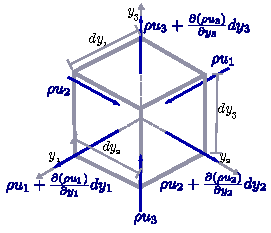
\includegraphics[scale=1.5,trim=0cm 0.0cm 0cm 0.0cm, clip=true]{Imagens/Cap2/volInf_fluxoMassa.pdf}	
	\caption{Volume de controle infinitesimal: Fluxo de massa}
	\label{fig:volInf_fluxoMassa}
	%\vspace{-1em} % Diminui o espaço antes da figura
\end{figure}


\begin{align}
	\begin{split}
	\frac{\partial \density}{\partial t}\deriv V =& \left(\density u_1 \deriv A_{1}  +  \density u_2 \deriv A_{2} + \density u_3  \deriv A_{3} \right) - \\  &\left(\left(\density u_1 + \frac{\partial \density u_1}{\partial y_1}\deriv y_1 \right)\deriv A_{1} + \left(\density u_2+ \frac{\partial \density u_2}{\partial y_2}\deriv y_2 \right) \deriv A_{2} + \left(\density u_3 + \frac{\partial \density u_3}{\partial y_3}\deriv y_3 \right) \deriv A_{3}\right), \label{eq:conser_massa_0} 
	\end{split}
\end{align}

\noindent com $\density$ a massa específica do fluido e $\deriv A_{i}$ a área referente à face ortogonal ao eixo $y_i$. Considerando que $\deriv V = \deriv y_1 \deriv y_2 \deriv y_3 = \deriv y_1 \deriv A_1 = \deriv y_2 \deriv A_2 = \deriv y_3 \deriv A_3 $  e manipulando-se algebricamente a Eq. \ref{eq:conser_massa_0} chega-se a seguinte expressão:

\begin{align}
	\frac{\partial \density}{\partial t} = - \frac{\partial \density u_{1}}{\partial y_1} - \frac{\partial \density u_{2}}{\partial y_2}- \frac{\partial \density u_{3}}{\partial y_3}.
\end{align}

Para escoamentos incompressíveis, quando $\density$ é constante ao longo do tempo, a equação fica reduzida a:

\begin{align}
	 \frac{\partial u_{1}}{\partial y_1} + \frac{\partial u_{2}}{\partial y_2} + \frac{\partial u_{3}}{\partial y_3} = 0, 
\end{align} 

\noindent ou ainda:

\begin{align}
	\divergence \cdot \velocity = 0.
	\label{eq:conser_massa_incom} 
\end{align} 

\subsection{Equação da quantidade de movimento}


Para um volume de controle infinitesimal, a lei da conservação da quantidade de movimento afirma que a variação temporal da quantidade de movimento no interior do volume é determinada pela diferença entre o fluxo de quantidade de movimento que entra e o que sai pelas suas fronteiras, somada à resultante das forças aplicadas sobre o volume de controle.

Para chegar-se à equação da quantidade de movimento em sua forma conservativa partindo desse princípio, inicia-se com a avaliação das forças que atuam sobre um volume de controle infinitesimal no instante atual. Considerando o equilíbrio das forças externas e internas na direção $y_1$, de acordo o volume apresentado na Fig. \ref{fig:volInf_tensao}, chega-se na seguinte relação:


\begin{align}
	\begin{split}
	F_1 =& -\left(\stress_{11}\deriv y_2 \deriv y_3 + \stress_{12}\deriv y_1 \deriv y_3 + \stress_{13}\deriv y_1 \deriv y_2\right) + \\ & \left(\left(\stress_{11} + \frac{\partial \stress_{11}}{\partial y_1}\deriv y_1 \right)\deriv y_2 \deriv y_3 + \left(\stress_{12}+ \frac{\partial \stress_{12}}{\partial y_2}\deriv y_2\right)\deriv y_1 \deriv y_3 + \left(\stress_{13}+ \frac{\partial \stress_{13}}{\partial y_3}\deriv y_3\right)\deriv y_1 \deriv y_2\right) + \\& b_{1}\deriv y_1 \deriv y_2 \deriv y_3, \label{eq:equil_forca_y1} 
	\end{split}
\end{align}	

\noindent onde $F_1$ representa a resultante das forças externas na direção $y_1$; $\stress_{ij}$ são as componentes $ij$ do tensor de tensões Cauchy ($\stresstensor$); e $b_1$ representa a componente na direção $y_1$ do vetor força de campo por unidade de volume $\mathbf{b}$. Dividindo-se Eq. \ref{eq:equil_forca_y1} por $\deriv V$ e efetuando as subtrações, têm-se a força resultante por unidade de volume ($q_1$) dada por:

\begin{align}
		q_1 =\frac{\partial \stress_{11}}{\partial y_1} + \frac{\partial \stress_{12}}{\partial y_2} + \frac{\partial \stress_{13}}{\partial y_3} + b_{1}.
\end{align}	

\begin{figure}[htb!]
	\centering 
	%\vspace{-1em} % Diminui o espaço antes da figura
	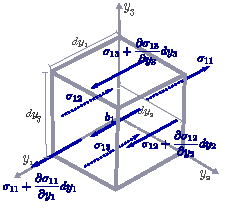
\includegraphics[scale=1.5,trim=0cm 0.0cm 0cm 0.0cm, clip=true]{Imagens/Cap2/volInf_tensao.pdf}	
	\caption{Volume de controle infinitesimal: Componentes de força na direção $y_1$}
	\label{fig:volInf_tensao}
	%\vspace{-1em} % Diminui o espaço antes da figura
\end{figure}

Considerando-se o equilíbrio das forças nas direções $y_2$ e $y_3$, pode-se escrever também:

\begin{align}
	q_2 =\frac{\partial \stress_{21}}{\partial y_1} + \frac{\partial \stress_{22}}{\partial y_2} + \frac{\partial \stress_{23}}{\partial y_3} + b_{2},
\end{align}	

\begin{align}
	q_3 =\frac{\partial \stress_{31}}{\partial y_1} + \frac{\partial \stress_{32}}{\partial y_2} + \frac{\partial \stress_{33}}{\partial y_3} + b_{3},
\end{align}

\noindent ou ainda:

\begin{align}
	\mathbf{q} = \divergence \cdot \stresstensor + \mathbf{b}.
\end{align}


Realizando-se o balanço da quantidade de movimento no volume de controle infinitesimal da Fig. \ref{fig:volInf_consQtdeMov}, e aplicando-se a lei da conservação da quantidade de movimento, pode-se chegar a seguinte equação:


\begin{align}
	\begin{split}
	\frac{\partial \density \velocity}{\partial t}\deriv V =& u_1\density \velocity \deriv A_1 + u_2\density \velocity \deriv A_2 + u_3 \density \velocity \deriv A_3 - \\
	 & \left(\left(u_1 \density \velocity + \frac{\partial u_1 \density \velocity}{\partial y_1}\deriv y_1 \right)\deriv A_1 + \left(u_2 \density \velocity + \frac{\partial u_2 \density \velocity}{\partial y_2}\deriv y_2 \right)\deriv A_2 \right. + \\ & \left.   \left(u_3 \density \velocity + \frac{\partial u_3 \density \velocity}{\partial y_3}\deriv y_3 \right)\deriv A_3\right) + \mathbf{q} \deriv V,
	\label{eq:QM_0} 
	\end{split}
\end{align}	

\noindent dividindo-se a Eq. \ref{eq:QM_0} por $\deriv V$ e efetuando-se as subtrações, chega-se a:

\begin{align}
		\frac{\partial \density \velocity}{\partial t} = 
		-\frac{\partial u_1 \density \velocity}{\partial y_1} 
		-\frac{\partial u_2 \density \velocity}{\partial y_2}  
		-\frac{\partial u_3 \density \velocity}{\partial y_3} + \mathbf{q},
		\label{eq:QM_1} 
\end{align}

ou ainda:

\begin{align}
	\density\left(\frac{\partial\velocity}{\partial t} + \divergence \cdot \left(\velocity\otimes\velocity\right) - \sbodyforce \right) - \divergence \cdot \stresstensor  &= \vzero, \label{eq:QM_2} 
\end{align}

\noindent com $\sbodyforce = \density \mathbf{b}$ que representa a força de campo por unidade de massa.

\begin{figure}[htb!]
	\centering 
	%\vspace{-1em} % Diminui o espaço antes da figura
	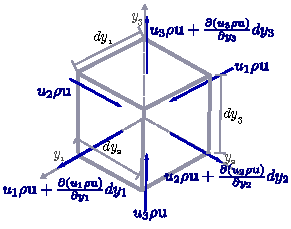
\includegraphics[scale=1.5,trim=0cm 0.0cm 0cm 0.0cm, clip=true]{Imagens/Cap2/volInf_consQtdeMov.pdf}	
	\caption{Volume de controle infinitesimal: Fluxo de quantidade de Movimento}
	\label{fig:volInf_consQtdeMov}
	%\vspace{-1em} % Diminui o espaço antes da figura
\end{figure}

Da consideração da equação da continuidade, a Eq. \ref{eq:QM_2} pode ser rescrita ainda em sua forma convectiva como:

\begin{align}
	\density\left(\frac{\partial\velocity}{\partial t} + \left( \velocity \cdot \gradient \right)  \velocity  - \sbodyforce \right) - \divergence \cdot \stresstensor = \vzero. \label{eq:Navier-Stokes} 
\end{align}

O tensor de tensões de Cauchy $\stresstensor$ é definido para fluidos newtonianos incompressíveis pela seguinte relação constitutiva:

\begin{align}
\stresstensor &= -\press \unittensor + 2\viscosity\straintensor(\velocity),\label{eq:tensor_tensoes_fluido}
\end{align}

\noindent onde $\press$ representa a pressão, $\viscosity$ a viscosidade dinâmica do fluido e $\straintensor(\bullet)$ é o tensor taxa de deformação infinitesimal, definido como:


\begin{align}
\straintensor(\bullet) = \frac{1}{2}\left(\gradient (\bullet) + \gradient (\bullet)^{T}\right). 
\label{eq:tensor_taxa_defor}
\end{align}

\subsection{Formulação forte da mecânica dos fluidos}

Seja $\domain \in \nrealspace$, com $\nsd = 2,3$, o domínio espacial que define o escoamento do fluido com contorno $\boundary = \GammaD \cup \GammaN$, no instante $t \in (0,\totalTime)$ (ver Fig. \ref{fig:dominioFluido}).

Para escoamentos incompressíveis isotérmicos o fluido possui movimento descrito pela equação da quantidade de movimento, ou equações de Navier-Stokes (Eq. \ref{eq:Navier-Stokes}) e da conservação de massa (Eq. \ref{eq:conser_massa_incom}). Para completar a formulação da mecânica dos fluidos, condições de contorno devem ser especificadas. Em geral, em uma dada parte do contorno espacial, condições de contorno essenciais (Dirichlet) ou naturais (Neumann) são aplicadas. Dessa forma, o escoamento é governado pelo seguinte conjunto de equações:

\begin{equation}
	\left\{
	\begin{array}{l}
		\density\left(\frac{\partial\velocity}{\partial t} + \velocity\cdot\gradient\velocity - \sbodyforce \right) - \divergence \cdot \stresstensor = \vzero \ \textrm{em} \ \domain\\
		\divergence \cdot \velocity = 0 \ \textrm{em} \ \domain\\
		\velocity = \velocityD \ \textrm{em} \ \GammaD \\
		\stresstensor \cdot \snormal = \surfaceLoad \ \textrm{em} \ \GammaN,
	\end{array} \label{eq:conj_eq_DFC}
	\right.
\end{equation}

\noindent sendo $\GammaD$ a porção do contorno com condições de contorno de Dirichlet, representadas pelo campo de velocidades $\velocityD$, e $\GammaN$ aquela com condições de contorno de Neumann, descritas pelas forças de superfície $\surfaceLoad$. A variável $\snormal$ representa o vetor unitário normal ao contorno $\Gamma_{N}$.

\begin{figure}[htb!]
	\centering 
	%\vspace{-1em} % Diminui o espaço antes da figura
	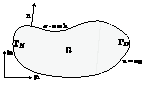
\includegraphics[scale=3.0,trim=0cm 0.0cm 0cm 0.0cm, clip=true]{Imagens/Cap2/dominioFluido.pdf}	
	\caption{Domínio para o problema da dinâmica dos fluidos computacional}
	\label{fig:dominioFluido}
	%\vspace{-1em} % Diminui o espaço antes da figura
\end{figure}

\section{Descrição Euleriana-Lagrangiana arbitrária (ALE)} \label{capitulo:Cap2:ALE}

A descrição Lagrangiana-Euleriana arbitrária \cite{DoneaGH:1982} representa uma generalização da descrição puramente Lagrangiana e da descrição puramente Euleriana do movimento do contínuo. A descrição Lagrangiana fixa a atenção em pontos materiais do contínuo, enquanto que na descrição Euleriana considera-se uma porção fixa do espaço ocupada pelo contínuo, e analisam-se os pontos materiais que passam por essa porção ao longo do tempo. Como consequência, na descrição puramente Lagrangiana a malha computacional move-se com o contínuo, enquanto que na Euleriana a malha computacional mantém-se fixa. Por sua vez, na descrição Lagrangiana-Euleriana arbitrária, trabalha-se com pontos de referência que podem movimentar-se, mas de maneira independente do movimento dos pontos materiais do contínuo analisado.

Para a aplicação dessa metodologia às equações governantes da mecânica dos fluidos é importante a definição de três domínios, de acordo com a Fig. \ref{fig:dominioAle}. O domínio inicial, chamado de \textbf{domínio material} ($\domainMat$), que é definido pelas coordenadas dos pontos materiais $\posMat$; O domínio atual, chamado de \textbf{domínio espacial} ($\domain$), definido pelas coordenadas $\pos$; e por fim, o \textbf{domínio de referência} ($\domainRef$) com coordenadas dos pontos de referência $\posALE$. 

Considera-se nesse texto, o domínio de referência, $\domainRef$, como sendo a configuração inicial da malha, enquanto que a configuração atual da malha e do contínuo consistem ambas na referência espacial $\domain$.

As coordenadas no domínio atual do contínuo, $\domain$, podem ser mapeadas a partir do domínio inicial ($\domainMat$) ou a partir do domínio de referência ($\domainRef$) utilizando as seguintes funções de mapeamento:  

\begin{align}
	\pos = \fmapAI(\posMat,t) = \fmapAR(\posALE,t).
\end{align}

\begin{figure}[htb!]
	\centering
	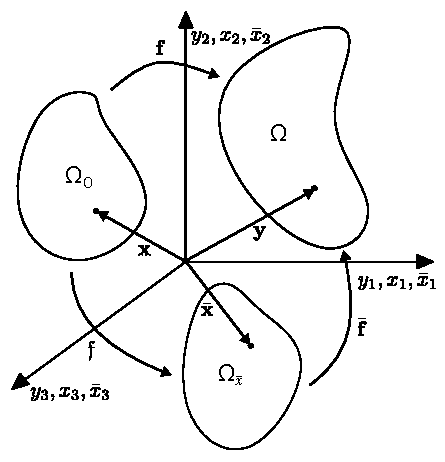
\includegraphics[scale=1.0]{Imagens/Cap2/dominioALE.pdf}	
	\caption{Domínios utilizados para a descrição Lagrangiana-Euleriana arbitrária}
	\label{fig:dominioAle}
\end{figure}

Da mesma forma, o domínio de referência, pode ser mapeado a partir do domínio inicial por:

\begin{align}
	\posALE = \fmapRI(\posMat,t).
\end{align}

A velocidade dos pontos da malha é calcula por:

\begin{align}
	\velocityALE = \left. \frac{\partial \fmapAR(\posALE,t)}{\partial t} \right|_{\posALE},
\end{align}

\noindent e a velocidade dos pontos materiais no instante $t$ é obtida pela derivada do vetor posição $\pos$ mantendo $\posMat$ fixo:

\begin{align}
	\velocity = \left. \frac{\partial \fmapAI(\posMat,t)}{\partial t} \right|_{\posMat} = \left. \frac{\partial \pos(\posMat,t)}{\partial t} \right|_{\posMat}.
\end{align}


As matrizes jacobianas dos mapeamentos considerando a dependência do espaço e do tempo são dadas por:

\begin{equation} 
	\FmapAI = \frac{\partial \left(\fmapAI(\posMat,t),t\right)}{\partial (\posMat,t)}=
	\begin{bmatrix}
		\frac{\partial {\pos}}{\partial {\posMat}} & \velocity \\
		\vzero^T & 1 \\
	\end{bmatrix}
	\text{,}
\end{equation}

\begin{equation} 
	\FmapAR = \frac{\partial \left(\fmapAR(\posALE,t),t\right)}{\partial (\posALE,t)}=
	\begin{bmatrix}
		\frac{\partial {\pos}}{\partial {\posALE}} & \velocityALE \\
		\vzero^T & 1 \\
	\end{bmatrix}
	\text{,}
\end{equation}

e

\begin{equation}
	\FmapRI = \frac{\partial \left({\fmapRI}(\posMat,t),t\right)}{\partial (\posMat,t)}=
	\begin{bmatrix}
		\frac{\partial {\posALE}}{\partial {\posMat}} & \mathbf{w} \\
		\vzero^T & 1 \\
	\end{bmatrix}
	\text{,}
\end{equation}

\noindent sendo $\mathbf{w} = \left. \frac{\partial \posALE}{\partial t} \right|_{\posMat}$.


Considerando que $\fmapAI\left(\posMat,t\right) = \fmapAR \circ \fmapRI$, pode-se escrever:

\begin{align}
	\frac{\partial(\fmapAI(\posMat,t),t)}{\partial(\posMat,t)} = \frac{\partial(\fmapAR(\posALE,t),t)}{\partial(\posALE,t)} \cdot \frac{\partial(\fmapRI(\posMat,t),t)}{\partial(\posMat,t)},
\end{align}

\noindent que pode ser rescrita como:

\begin{align}
	\begin{bmatrix}
		\frac{\partial {\pos}}{\partial {\posMat}} & \velocity \\
		\vzero^T & 1 \\
	\end{bmatrix}
	=
	\begin{bmatrix}
		\frac{\partial {\pos}}{\partial {\posALE}} & \velocityALE \\
		\vzero^T & 1 \\
	\end{bmatrix}
	\cdot
	\begin{bmatrix}
		\frac{\partial {\posALE}}{\partial {\posMat}} & \mathbf{w} \\
		\vzero^T & 1 \\
	\end{bmatrix} .
\end{align}

Dessa forma, pode-se estabelecer uma relação entre a velocidade da malha e a velocidade do ponto material:

\begin{align}
	\velocity = \velocityALE + \frac{\partial{\pos}}{\partial{\posALE}}\cdot \mathbf{w} \label{eq:vel_rel_mat_ALE}
\end{align}

Supondo agora uma grandeza física escalar, denominada de $g(\pos,t)$ na configuração espacial, de $g^{*}(\posALE,t)$ na configuração de referência, e $g^{**}(\posMat,t)$ na configuração material. Pode-se escrever então:

\begin{align}
	g^{**}(\posMat,t) = g(\fmapAI(\posMat,t),t), 
\end{align}

\noindent ou:

\begin{align}
	g^{**} = g  \circ \fmapAI,
\end{align}

\noindent o que permite escrever o seguinte gradiente:

\begin{align}
	\frac{\partial g^{**}(\posMat,t)}{\partial (\posMat,t)} = \frac{\partial g(\pos,t)}{\partial (\pos,t)} \cdot \frac{\partial \fmapAI(\posMat,t)}{\partial (\posMat,t)},
\end{align}

\noindent que em forma matricial é apresentado como:

\begin{align}
	\begin{bmatrix}
		\frac{\partial {g^{**}}}{\partial {\posMat}} & \frac{\partial {g^{**}}}{\partial t} \\
	\end{bmatrix}
	=
	\begin{bmatrix}
		\frac{\partial {g}}{\partial \pos} & \frac{\partial {g}}{\partial t} 
	\end{bmatrix}
	\cdot
	\begin{bmatrix}
		\frac{\partial {\pos}}{\partial {\posMat}} & \velocity \\
		\vzero^T & 1 \\
	\end{bmatrix} .
\end{align}

Essa expressão nos permite escrever a derivada temporal da variável na configuração material:

\begin{align}
	\frac{\partial g^{**}}{\partial t} = \frac{\partial g}{\partial t} + \frac{\partial g}{\partial \pos} \cdot \velocity, 
\end{align}

\noindent que é justamente a derivada material de g. Para facilitar a visualização pode tirar os sobrescritos $**$, e então:

\begin{align}
	\frac{Dg}{Dt} = \left . \frac{\partial g}{\partial t} \right|_{\posMat} = \left . \frac{\partial g}{\partial t} \right|_{\pos} + \velocity \cdot \gradient g. \label{eq:der_mat}
\end{align}

Usando essa mesma metodologia pode-se escrever a transformação de $g^{*}(\posALE,t)$ para a referência material da seguinte forma:


\begin{align}
	g^{**} = g^{*}  \circ \fmapRI,
\end{align}

\noindent que resulta no seguinte gradiente

\begin{align}
	\begin{bmatrix}
		\frac{\partial {g^{**}}}{\partial {\posMat}} & \frac{\partial {g^{**}}}{\partial t} \\
	\end{bmatrix}
	=
	\begin{bmatrix}
		\frac{\partial {g^*}}{\partial \posALE} & \frac{\partial {g*}}{\partial t} 
	\end{bmatrix}
	\cdot
	\begin{bmatrix}
		\frac{\partial {\posALE}}{\partial {\posMat}} & \mathbf{w} \\
		\vzero^T & 1 \\
	\end{bmatrix},
\end{align}


\noindent com a segunda coluna resultando em:

\begin{align}
	\frac{\partial g^{**}}{\partial t} = \frac{\partial g^*}{\partial t} + \frac{\partial g*}{\partial \posALE} \cdot \mathbf{w}. \label{eq:ref_mat}
\end{align}

Utilizando-se a expressão apresenta na Eq. \ref{eq:vel_rel_mat_ALE} e substituindo-a em \ref{eq:ref_mat}, resulta em:

\begin{align}
	\frac{\partial g^{**}}{\partial t} = \frac{\partial g^*}{\partial t} + \frac{\partial g*}{\partial \pos} \cdot \left(\velocity - \velocityALE \right). 
\end{align}

Removendo-se os sobrescritos (**) e (*), chega-se a equação fundamental para os desenvolvimentos utilizando a metodologia ALE:

\begin{align}
	\frac{Dg}{Dt} = \left . \frac{\partial g}{\partial t} \right|_{\posMat} = \left . \frac{\partial g}{\partial t} \right|_{\posALE} + \left(\velocity - \velocityALE \right) \cdot \gradient g. \label{eq:der_mat_ALE}
\end{align}

Utilizando-se a definição de derivada material da Eq. \ref{eq:der_mat} e comparando com a Eq. \ref{eq:Navier-Stokes}, pode-se rescrever a equação da quantidade de movimento da seguinte forma:

\begin{align}
	\density\left(\frac{D\velocity}{Dt} - \sbodyforce \right) - \divergence \cdot \stresstensor &= \vzero. \label{eq:Navier-Stokes_der_mat_Euleriana}
\end{align}

Para expressar então a equação da quantidade de movimento em uma descrição Euleriana-Lagrangeana, basta substituir na Eq. \ref{eq:Navier-Stokes_der_mat_Euleriana} a definição de derivada material apresentada na Eq. \ref{eq:der_mat_ALE}, e têm-se finalmente:

\begin{align}
	\density\left(\left. \frac{\partial\velocity}{\partial t} \right|_{\posALE} + \left(\velocity - \velocityALE \right) \cdot \gradient  \velocity  - \sbodyforce \right) - \divergence \cdot \stresstensor = \vzero. \label{eq:Navier-Stokes_ALE} 
\end{align}

A equação da continuidade independe da movimentação da malha. Dessa forma a Eq. \ref{eq:conser_massa_incom} se mantém a mesma para as análises usando uma descrição ALE. Assim, reescrevendo o conjunto de equações da DFC apresenta na Eq. \ref{eq:conj_eq_DFC} para um descrição ALE, têm-se:

\begin{equation}
	\left\{
	\begin{array}{l}
		\density\left( \left. \frac{\partial\velocity}{\partial t} \right|_{\posALE}  + \left(\velocity - \velocityALE \right)\cdot\gradient\velocity - \sbodyforce \right) - \divergence \cdot \stresstensor = \vzero  \ \textrm{em} \ \domain\\
		\divergence \cdot \velocity = 0  \ \textrm{em} \ \domain\\
		\velocity = \velocityD \ \textrm{em} \ \GammaD \\
		\stresstensor \cdot \snormal = \surfaceLoad \ \textrm{em} \ \GammaN,
	\end{array} \label{eq:conj_eq_DFC_ALE}
	\right.
\end{equation}


\section{Forma fraca e discretização espacial das equações governantes} \label{capitulo:Cap2:FormaFraca}

Tomando-se a forma forte das equações governantes da DFC em descrição ALE, aplica-se o método de resíduos ponderados para se chegar à forma fraca e proceder com a discretização espacial. Os espaços de dimensão finita das funções tentativa que descrevem a velocidade e a pressão são chamados de $\usolution$ e $\psolution$ respectivamente, e definidos como:

\begin{align}
\usolution = \left\{\velocity \left . \right| \velocity \left(\cdot,t\right) \in \left(H^{1}\left(\domain\right)\right)^{\nsd}, \velocity = \velocity_D \ \textrm {em} \ \GammaD \right\}
\end{align}

\noindent e

\begin{align}
\psolution = \left\{\press \left . \right| \press \left(\cdot\right) \in L^{2}\left(\domain\right), \int_{\domain}\press \textrm { } \deriv \domain = 0 \textrm { se } \boundary = \GammaN \right\},
\end{align}

\noindent sendo $\left(H^{1}\left(\domain\right)\right)^{\nsd}$ o espaço de funções vetoriais com derivadas de quadrado integrável sobre $\domain$ e $L^{2}\left(\domain\right)$ o espaço de funções escalares que são de quadrado integrável sobre $\domain$.

O espaço das funções teste ou funções peso das equações da quantidade de movimento e da continuidade são definidos respectivamente por:

\begin{align}
\uweighting = \left\{\utest \left . \right| \utest \left(\cdot\right) \in \left(H^{1}\left(\domain\right)\right)^{\nsd}, \utest = \vzero \textrm { em} \ \GammaD \right\},
\end{align}


\begin{align}
\pweighting = \psolution.
\end{align}

Aplicando-se o método dos resíduos ponderados sobre as equações Eq. \eqref{eq:Navier-Stokes_ALE} e Eq.\eqref{eq:conser_massa_incom}, integrando-se por partes o termo referente ao tensor de tensões de Cauchy, empregando-se o teorema da divergência e levando-se em consideração a condição de homogeneidade da função $\utest$ sobre o contorno $\GammaD$, obtém-se a forma fraca. A solução do problema consiste então em encontrar $\velocity \in \usolution$ e $\press \in \psolution$, de tal modo que $\forall$ $\utest \in \uweighting$ e $\ptest \in \pweighting$, as seguintes expressões sejam verdadeiras:


\begin{align}
\int_{\domain} \utest \cdot \density  \left(\left . \frac{\partial\velocity}{\partial t} \right|_{\posALE} + \left(\velocity - \velocityALE \right)\cdot\gradient \velocity - \sbodyforce \right) \deriv \domain + \int_{\domain} \straintensor(\utest) : \stresstensor  \deriv \domain - \int_{\GammaN} \utest \cdot \surfaceLoad \deriv\GammaN  \  &= 0,  \label{eq:QM_forma_fraca_0_cap2} 
\end{align}

\begin{align}
\int_{\domain} \ptest \left(\divergence \cdot \velocity\right) \deriv \domain &= 0. \label{eq:C_forma_fraca_0_cap2} 
\end{align}


\subsection{Método dos elementos finitos }

Antes de prosseguir com a discretização espacial da forma fraca do conjunto de equações da Mecânica dos Fluidos, é fundamental compreender os princípios básicos do Método dos Elementos Finitos.  A discretização espacial tanto pelo método dos elementos finitos, como pela técnica de análise isogeométrica (Cap. \ref{capitulo:Cap3}), consiste em, dado um problema com domínio $\domain$, dividi-lo em subdomínios $\domainE$, também chamados de elementos ou células, de forma que:

\begin{align}
	\domain \approx \domainh = {\bigcup_{e = 1}^{\nel}} \domainE,
\end{align}

\noindent onde $\domainh$ é o domínio discretizado por subdomínios, com o índice $h$ se referindo ao tamanho representativo dos elementos, e $\nel$ representando o número total de elementos.

Da mesma forma o contorno do domínio também é discretizado da seguinte forma:

\begin{align}
	\boundary \approx \boundaryh = {\bigcup_{b = 1}^{\neb}} \boundary^{b},
\end{align}

\noindent onde $\neb$ representa o número de elementos que formam o contorno.

No Método dos Elementos Finitos, cada subdomínio, denominado elemento, é composto por um conjunto de pontos, chamados nós. As variáveis de interesse do problema, que incluem a geometria na abordagem isoparamétrica, são aproximadas pela combinação linear de um número finito de funções associadas aos nós, chamadas funções de forma, multiplicadas por variáveis chamadas parâmetros nodais. As funções de forma utilizadas no Método dos Elementos Finitos satisfazem, em geral, a propriedade de partição da unidade, ou seja, a soma das funções de forma associadas a todos os nós de um elemento resulta em 1 para qualquer ponto dentro do domínio paramétrico do elemento. A técnica de elementos finitos pode ser estudada nos diversos livros disponíveis sobre o assunto, tais como \citeonline{ZienkiewiczT:2005a,Reddy:2006}.

Nesse trabalho são utilizadas funções de forma quadráticas do tipo polinômios de Lagrange, sendo empregados elementos isoparamétricos triangulares para o caso 2D e tetraédricos para o caso 3D. Na Fig. \ref{fig:elementoFinito2d} e Fig. \ref{fig:elementoFinito3d}, pode-se observar os elementos finitos 2D e 3D respectivamente bem como os espaços paramétricos adimensionais adotados para definir as funções de forma. 

\begin{figure}[!htb]
	\centering	
	\subfloat[Elemento Finito 2d\label{fig:elementoFinito2d}]{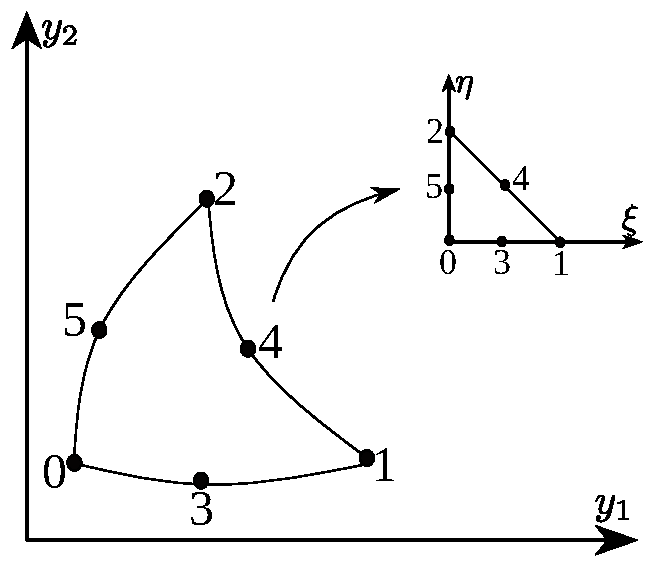
\includegraphics[scale=0.5,trim=0cm 0cm 0cm 0cm, clip=true]{Imagens/Cap2/elementoFinito2d.pdf}}\\
	\subfloat[Elemento Finito 3d\label{fig:elementoFinito3d}]{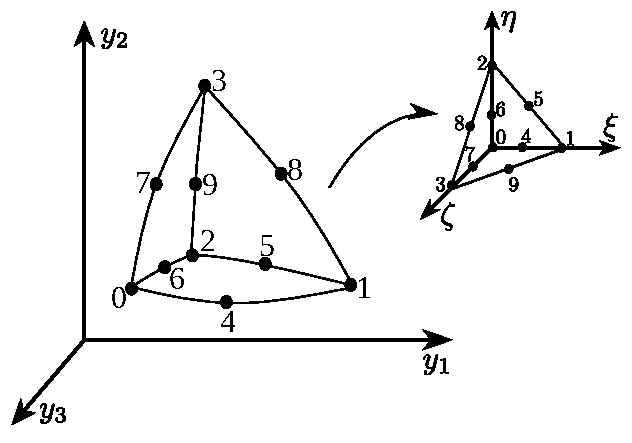
\includegraphics[trim=0 0 0 0,clip,scale=0.65]{Imagens/Cap2/elementoFinito3d.pdf}}
	\caption{Elementos Finitos: representação espacial e paramétrica}
\end{figure}

Adotar a abordagem isoparamétrica implica que a geometria do problema é descrita também pela combinação entre funções de forma e as coordenadas nodais da malha, conforme equação abaixo:

\begin{align}
	\pos^{h} = \sum_{A = 1}^{\nnos} \pos_{A}\shapef_{A}(\pos),
\end{align}

\noindent sendo que para uma geometria tridimensional o vetor $\pos$ possui coordenadas $y_1,y_2$ e $y_3$, as quais representam as posições físicas do domínio; O subíndice "$A$" $ \ $ representa o índice dos nós da malha, $\nnos$ o número total de nós e $\shapef$ as funções de forma da discretização.

A discretização das variáveis de interesse para DFC no contexto do método dos elementos finitos serão apresentados no seguinte capítulo (Cap. \ref{capitulo:Cap2:DiscEspacial}).


\subsection{Discretização Espacial} \label{capitulo:Cap2:DiscEspacial}

Os espaços de função tentativa para velocidade e pressão, bem como as funções teste, no contexto dos método dos elementos finitos, são dados pela combinação linear de parâmetros nodais com funções de forma definidas sobre cada subdomínio, atendendo à partição da unidade, de forma que o problema da dinâmica dos fluidos fica definido como: encontrar $\velocityh \in \usolutionh$ e $\pressh \in \psolutionh$, de tal modo que $\forall$ $\utesth \in \uweightingh$ e $\ptesth \in \pweightingh$ a seguinte expressão seja verdadeira:

\begin{align}
	\begin{split}
		&\int_{\domain} \utesth \cdot \density \left(\left. \frac{\partial\velocityh}{\partial t} \right|_{\posALE} + \left(\velocityh - \velocityALEh \right)\cdot\gradient \velocityh - \sbodyforceh \right) \deriv \domain + \int_{\domain} \straintensor(\utesth) : \stresstensor\left(\velocityh,\pressh \right)  \deriv \domain\\ & - \int_{\GammaN} \utesth \cdot \surfaceLoadh \deriv \GammaN \ + \int_{\domain} \ptesth \left(\divergence \cdot \velocityh\right) d \domain = 0,  \label{eq:QM_C_forma_fraca_1} 
	\end{split}
\end{align}

\noindent onde:

\begin{align}
\velocityh(\pos,t) = \sum_{A = 1}^{\nnos} \velocity_{A}(t)\shapef_{A}(\pos), \label{eq:interp_vel}
\end{align}

\begin{align}
\pressh(\pos,t)  = \sum_{A = 1}^{\nnos} \press_{A}(t)\shapef_{A}(\pos),\label{eq:interp_press} 
\end{align}

\begin{align}
\utesth(\pos)  = \sum_{A = 1}^{\nnos} \utest_{A}\shapef_{A}(\pos), \label{eq:interp_utest}
\end{align}

\begin{align}
\ptesth(\pos)  = \sum_{A = 1}^{\nnos} \ptest_{A}\shapef_{A}(\pos), \label{eq:inter_ptest} 
\end{align}

\noindent sendo as variáveis $\utest_{A}$ e $\ptest_{A}$ arbitrárias nas aproximações.

No entanto, as formulações obtidas pelo método de Galerkin são conhecidas por apresentarem oscilações espúrias em escoamentos dominados pela convecção. Uma das formas de se lidar com esse problema é a utilização de métodos estabilizados, como \textit{Streamline-Upwind/Petrov-Galerkin} (SUPG) \cite{BrooksH:1982, HughesT:1984}, aplicado nesse trabalho. Essa metodologia consiste em adicionar à equação da quantidade de movimento, o seu resíduo ponderado por $\SUPG \left(\left(\velocityh - \velocityALEh \right) \cdot \gradient \utesth\right)$, onde $\SUPG$ é um parâmetro de estabilização. Do ponto de vista numérico a aplicação de  sobre o termo convectivo da equação da quantidade de movimento dá origem a um termo difusivo adicional, cuja viscosidade tem magnitude $\SUPG$, e é responsável por garantir a estabilidade numérica em problemas com convecção dominante.

Para os problemas de escoamentos incompressíveis aqui analisados, deve-se levar em conta que os campos de velocidade e pressão não podem ser aproximados arbitrariamente, podendo levar à ocorrência de oscilações espúrias no campo de pressão. Para evitar isso, podem ser escolhidos elementos Taylor-Hood que obedeçam, à condição de \textit{Ladyzhenskaya-Babuška-Brezzi} (LBB) \cite{BrezziF:1991,ZienkiewiczTN:2005,StrangF:2008}, ou pode-se recorrer a um método estabilizado. 

Neste trabalho, para estabilização da pressão, emprega-se a técnica \textit{Pressure Stabilization Petrov Galerkin} (PSPG)   \cite{HughesFB:1986,TezduyarMRS:1992a}. Essa técnica consiste em adicionar à equação da continuidade, o resíduo da equação da quantidade de movimento ponderada pela função $\PSPG \left(\frac{\gradient \ptesth}{\density}\right)$, onde $\PSPG$ é um parâmetro de estabilização. Essa estabilização cria termos dependentes da pressão na equação da continuidade, responsáveis pela flexibilização do campo de pressão e por contornar a condição LBB.

Por fim, para prover maior estabilização em problemas com formação de vórtices, adiciona-se à equação da quantidade de movimento o resíduo da equação da continuidade ponderado por $ \LSIC \density \left(\divergence \cdot \utesth\right)$ \cite{TezduyarO:2000}, sendo $\LSIC$ um parâmetro de estabilização. A estabilização  $\LSIC$ dá origem a um termo do tipo mínimos quadrados, e que também introduz na formulação uma difusão artificial.

Nota-se que a consistência da formulação estabilizada é garantida, uma vez que são adicionados às equações seus resíduos ponderados. Os parâmetros de estabilização $\SUPG$, $\PSPG$ e $\LSIC$ têm função de proporcionar uma solução estável e otimizar a convergência durante o refinamento de malha. A obtenção dos parâmetros estabilizadores será discutida na Subseção \ref{capitulo:Cap2:FormaFraca:taus}. 

Por fim, o problema da dinâmica dos fluidos passa a ser a determinação de $\velocityh \in \usolutionh$ e $\pressh \in \psolutionh$, de tal modo que $\forall$ $\utesth \in \uweightingh$ e $\ptesth \in \pweightingh$ as seguintes expressões sejam verdadeiras:

\begin{align}
\begin{split}
&\int_{\domain} \utesth \cdot \density\left(\left. \frac{\partial\velocityh}{\partial t}\right|_{\posALE}+ \left(\velocityh - \velocityALEh \right) \cdot \gradient \velocityh - \sbodyforceh\right) \deriv \domain +\int_{\domain} \straintensor \left(\utesth\right) : \stresstensor \left(\velocityh,\pressh\right)\ \deriv \domain\\ &
- \int_{\GammaN}\utesth \cdot \surfaceLoadh \ \deriv \GammaN 
+ \sum_{e=1}^{\nel} \int_{\domainE} \SUPG \left(\left(\velocityh - \velocityALEh \right) \cdot \gradient \utesth\right) \cdot \resMom\left(\velocityh,\pressh \right)\  \deriv \domain\\
&+ \sum_{e=1}^{\nel} \int_{\domainE} \density \LSIC \divergence \cdot \utesth \resPre\left(\velocityh\right)\  \deriv \domain = 0,
\label{eq:QM_forma_fraca}
\end{split}
\end{align}

\noindent e

\begin{align}
	\begin{split}
	&\int_{\domain}\ptesth \divergence \cdot \velocityh \ \deriv \domain
	+ \sum_{e=1}^{\nel} \int_{\domainE} \PSPG \left(\frac{\gradient \ptesth}{\density}\right) \cdot \resMom\left(\velocityh,\pressh\right) \  \deriv \domain = 0,
	\label{eq:C_forma_fraca}
	\end{split}
	\end{align}

\noindent onde $\resMom$ e $\resPre$ são os resíduos da equação da quantidade de movimento e da equação da continuidade, respectivamente, dados por:

\begin{align}
\resMom\left(\velocityh,\pressh\right)&=\density\left(\left. \frac{\partial\velocityh}{\partial t}\right|_{\posALE}+\left(\velocityh - \velocityALEh \right)\cdot \gradient \velocityh - \sbodyforceh\right) - \divergence \cdot \stresstensor\left(\velocityh,\pressh\right),
\end{align}

\noindent

\begin{align}
\resPre\left(\velocityh\right)&=\divergence \cdot \velocityh.
\end{align}

A solução de modelos móveis requer a utilização de uma técnica adequada para movimentação da malha local. A técnica utilizada nesse trabalho é conhecida como MJBS (Mesh-Jacobian Based Stiffening) introduzida por \citeonline{TezduyarBSJ:1992f} e será abordada na Subseção \ref{capitulo:Cap7:CondAcop:MovMalha}.

Visto que existem funções teste separadas para a velocidade e pressão, pode-se definir dois vetores residuais correspondentes a equação da quantidade de movimento ($\NNSM$) e a equação da continuidade ($\NNSC$). Considerando a arbitrariedade de $\utest_{A}$ e $\ptest_{A}$, têm-se:

\begin{align}
\NNSM  = [\left(\NNSM\right)_{A,i}],
\end{align}

\begin{align}
\NNSC =  [\left(\NNSC\right)_{A}],
\end{align}
	
\noindent com:

\begin{align}
	\begin{split}
	\left(\NNSM\right)_{A,i} =&\int_{\domain} \shapef_{A}\mathbf{e_i} \cdot \density\left(\left. \frac{\partial\velocityh}{\partial t}\right|_{\posALE}+\left(\velocityh - \velocityALEh \right)\cdot \gradient \velocityh - \sbodyforceh\right) \deriv \domain +\int_{\domain} \straintensor \left(\shapef_{A}\mathbf{e_i}\right) : \stresstensor \left(\velocityh,\pressh\right)\ \deriv \domain\\ &
	- \int_{\GammaN}\shapef_{A}\mathbf{e_i} \cdot \surfaceLoadh \ \deriv \GammaN 
	+ \sum_{e=1}^{\nel} \int_{\domainE} \SUPG \left(\left(\velocityh - \velocityALEh \right) \cdot \gradient \shapef_{A}\mathbf{e_i}\right) \cdot \resMom\left(\velocityh,\pressh \right)\  \deriv \domain\\
	&+ \sum_{e=1}^{\nel} \int_{\domainE} \density \LSIC \left(\divergence \cdot \shapef_{A}\mathbf{e_i}\right) \resPre\left(\velocityh\right)\  \deriv \domain  ,
	\end{split}
\end{align}

\noindent e:

\begin{align}
	\begin{split}
	\left(\NNSC\right)_{A} = &\int_{\domain} \shapef_{A} \divergence \cdot \velocityh \ \deriv \domain  
	+ \sum_{e=1}^{\nel} \int_{\domainE} \PSPG \left(\frac{\gradient \shapef_{A}}{\density}\right) \cdot \resMom\left(\velocityh,\pressh\right) \  \deriv \domain,
	\end{split}
\end{align}

\noindent com $i=1,2$ para problemas 2D e $i=1,3$ para problemas 3D.
		
Considerando $\Acceleration$, $\Velocity$ e $\Press$ os vetores nodais dos graus de liberdade respectivos a velocidade, aceleração e pressão, pode-se escrever a forma semidiscreta do problema da DFC como: Encontrar $\Acceleration$, $\Velocity$ e $\Press$ de maneira que

\begin{align}
\NNSM(\Acceleration,\Velocity,\Press) = \vzero,\label{eq:resid_semi_discr_QM}
\end{align}

\noindent e

\begin{align}
\NNSC(\Acceleration,\Velocity,\Press) = \vzero. \label{eq:resid_semi_discr_C}
\end{align}



\subsection{Parâmetros de estabilização}\label{capitulo:Cap2:FormaFraca:taus}

Considerando que nesse trabalho dois tipos de aproximações espaciais são utilizadas, uma baseada no FEM e outra baseada em IGA, adotam-se os parâmetros propostos por \citeonline{TakizawaTO:2018} e \citeonline{OtoguroTT:2020}, que são adequados para ambas aproximações. 

Para essa opção é necessário definir-se o tensor métrico do elemento no espaço. Para isso, inicia-se com a definição da matriz Jacobiana $\matrixQ$, dada por:

\begin{align}
	\matrixQ&=\left(\frac{\partial\pos}{\partial\coordAdimen}\right),
\end{align}

\noindent com $\coordAdimen$ representando as coordenadas do espaço paramétrico, com componentes $\xi_1, \xi_2$ e $\xi_3$.

Para que a ordem polinomial seja levada em consideração na determinação dos parâmetros de estabilização, aplica-se uma mudança de escala na matriz $\matrixQ$, através da matriz $\matrixD$, conforme a seguinte expressão:

\begin{align}
	\matrixQhat&=\matrixQ\matrixD^{-1}.
\end{align}

Para elementos finitos com funções de forma polinomiais de Lagrange de ordem $p_{i}$, na direções $\xi_i$ do espaço paramétrico , com $-1\leq\xi_i\leq1$, a  matriz $\matrixD$ é definida como:


\textcolor{red}{e se a variação for de 0,1 ? tem alguma diferença}

\begin{align}
	\matrixD&=\begin{bmatrix}
		p_{\xi_1} & 0 & 0\\
		0 & p_{\xi_2} & 0 \\
		0 & 0 & p_{\xi_3}
	\end{bmatrix}.
\end{align}

A definição da matriz $\matrixD$ para elementos isogeométricos será descrita na Subseção \ref{capitulo:Cap3:RepreGeo:taus2}.

O comprimento direcional do elemento é definido como:

\begin{align}
	\RQD &=2\left(\rRGN\rRGN : \matrixG \right)^{-\frac{1}{2}},
\end{align}

\noindent sendo $\rRGN$ o vetor unitário na direção do gradiente da intensidade da velocidade e $\matrixG$ o tensor métrico do elemento, os quais são representados respectivamente como:

\begin{align}
	\rRGN&=\frac{\gradient \lVert\velocityh - \velocityALEh\rVert}{\lVert \gradient \lVert\velocityh - \velocityALEh\rVert\rVert} \label{eq:rRGN}
\end{align}

\noindent e

\begin{align}
	\matrixG &= \matrixQhat^{-T} \cdot \matrixQhat^{-1}. 
\end{align}

O comprimento do elemento é limitado pelos mínimos e máximos valores representados abaixo:

\begin{align}
	h_{min} \equiv 2\min_{r}\left((\rRGN\rRGN:\matrixG)^{-\frac{1}{2}} \right), \\
	h_{max} \equiv 2\max_{r}\left((\rRGN\rRGN:\matrixG)^{-\frac{1}{2}} \right),
\end{align}

\noindent que podem ser reescritos como:

\begin{align}
	h_{min} = 2\left(\lambda_{max}\matrixG\right)^{-\frac{1}{2}}, \\
	h_{max} = 2\left(\lambda_{min}\matrixG\right)^{-\frac{1}{2}},
\end{align}

\noindent onde $\lambda_{max}$ e $\lambda_{min}$ representam os máximos e mínimos autovalores da matriz $\matrixG$. 

Os parâmetros de estabilização são dados por:

\begin{align}
	\SUPG = \PSPG =\left(\frac{1}{\SUGNi^2} + \frac{1}{\SUGNii^2} + \frac{1}{\SUGNiii^2} \right)^{-\frac{1}{2}},
\end{align}

\begin{align}
	\LSIC = \frac{\RQD^2}{\SUPG},
\end{align}

\noindent onde:

\begin{align}
	\SUGNi^{-2} = \left(\velocityh - \velocityALEh \right) \left(\velocityh - \velocityALEh \right) : \matrixG ,
\end{align}

\begin{align}
	\SUGNii&=\frac{\timeStep}{2},
\end{align}

\noindent e

\begin{align}
	\SUGNiii^{-1} = \kviscosity \left(\rRGN_{reg}\rRGN_{reg} : \matrixG + \left(1 - \rRGN_{reg}^2)4h_{min}^{-2} \right)\right) ,
\end{align}

\noindent sendo $\rRGN_{reg}$ definido como:

\begin{align}
	\rRGN_{reg} =\frac{\gradient \lVert\velocityh - \velocityALEh\rVert}{\lVert \gradient \lVert\velocityh - \velocityALEh\rVert\rVert + \varepsilon\left(\lVert \gradient \lVert\velocityh - \velocityALEh\rVert\rVert\right)_0},
\end{align}

\noindent com $\varepsilon$ uma constante pequena e $\left(\lVert \gradient \lVert\velocityh- \velocityALEh\rVert\rVert\right)_0$ um valor de referência. Os termos $\SUGNi$, $\SUGNii$ e $\SUGNiii$ são parâmetros correspondentes aos termos convectivos, inerciais e viscosos, respectivamente.

\section{Integração Temporal}\label{capitulo:Cap2:IntegTemp}

Para a integração temporal das equações governantes, utiliza-se o método $\alpha$-generalizado. Esse método foi proposto inicialmente por \citeonline{ChungH:1993} no contexto da mecânica das estruturas, e foi estendido para o contexto da dinâmica dos fluidos computacional por \citeonline{JansenWH:2000}.

Considerando que o tempo da análise do problema é definido por um intervalo de $[0,\totalTime]$, o qual é particionado em subintervalos $\timeStep_{n} = t_{n+1} - t_{n}$, com $t_{n}$ e $t_{n+1}$ os instantes anterior e atual, respectivamente. A solução do problema consiste em: conhecida a solução nos graus de liberdade nodais ($\Acceleration$, $\Velocity$ e $\Press$) no passo de tempo $n$, encontrar a solução no passo de tempo $n+1$ de forma que:

\begin{align}
\NNSM(\Acceleration_{n+\alpham},\Velocity_{n+\alphaf},\Press_{n+1}) = \vzero, \label{eq:resid_QM_alpha}\\
\NNSC(\Acceleration_{n+\alpham},\Velocity_{n+\alphaf},\Press_{n+1}) = \vzero, \label{eq:resid_cont_alpha}
\end{align}

\noindent com:

\begin{gather}
\Acceleration_{n+\alpham} = \Acceleration_n + \alpham \left( \Acceleration_{n+1} - \Acceleration_n \right), \label{eq:inter_acel}\\
\Velocity_{n+\alphaf} = \Velocity_n + \alphaf \left( \Velocity_{n+1} - \Velocity_n \right), \label{eq:inter_vel}
\end{gather}

\noindent sendo $\Acceleration_{n+\alpham}$ e $\Velocity_{n+\alphaf}$ valores intermediários entre $t_{n}$ e $t_{n+1}$ do vetor aceleração e velocidade. A relação entre os valores nodais de aceleração e velocidade são calculados de acordo com fórmula discreta de Newmark (ver, por exemplo, \cite{Hughes:1976}):

\begin{gather}
\Velocity_{n+1} = \Velocity_n + \timeStep\left(\left(1-\gamma\right)\Acceleration_n + \gamma\Acceleration_{n+1} \right). \label{eq:Newmark}
\end{gather}

Os parâmetros que definem o instante intermediário, no qual as variáveis serão calculadas, são determinados de forma a proporcionarem estabilidade e precisão ao método. Seguindo a metodologia proposta por \citeonline{JansenWH:2000}, uma precisão de segunda ordem é obtida, para casos lineares, desde que: 

\begin{gather}
\gamma = 1/2 + \alpham - \alphaf,\label{eq:gamma}
\end{gather}

\noindent enquanto que a estabilidade do problema é incondicional com:

\begin{gather}
\alpham \ge \alphaf \ge 1/2.
\end{gather}

Para proporcionar a precisão de segunda-ordem de convergência e estabilidade da solução, pode-se calcular o parâmetro $\gamma$ de acordo com Eq. \ref {eq:gamma} e $\alpham$, $\alphaf$, através de \cite{Hughes:2000}:


\begin{gather}
\alpham = \frac{1}{2}\left(\frac{3 - \specRadius}{1+\specRadius}\right)\label{eq:alpha_m}\\
\end{gather}

\noindent e

\begin{gather}
\alphaf = \frac{1}{1+\specRadius}\label{eq:alpha_f}.
\end{gather}

O parâmetro $\specRadius$ é conhecido como raio espectral da matriz de amplificação quando $\timeStep_{n} \rightarrow \infty$. Esse parâmetro controla a dissipação numérica em altas frequências realizada pelo processo de integração e está contido no intervalo de $[0,1]$. Para $\specRadius = 0$ a dissipação é máxima e para $\specRadius = 1$ não há introdução de difusão numérica ao método.

Para a solução do sistema de equações não lineares compostas por Eq. \eqref{eq:resid_QM_alpha} e Eq. \eqref{eq:resid_cont_alpha} utiliza-se o método de Newton-Raphson. O método pode ser separado em duas etapas, uma etapa preditiva e outra iterativa corretiva \cite{BazilevsTT:2013}.

Na etapa preditiva, conhecida a solução em um passo de tempo $n$, prediz-se a solução em $n+1$ com as seguintes equações:

\begin{align}
\Acceleration_{n+1}^{0} = \frac{\gamma-1}{\gamma}\Acceleration_{n} \label{eq:pred_acel},
\end{align}

\begin{align}
\Velocity_{n+1}^{0} = \Velocity_{n}, \label{eq:pred_vel}
\end{align}

\begin{align}
\Press_{n+1}^{0} = \Press_{n},\label{eq:pred_press}
\end{align}

\noindent onde o índice $0$ representa a iteração de número zero. 

Na etapa iterativa corretiva, itera-se sobre a Eq. \eqref{eq:resid_QM_alpha} e Eq. \eqref{eq:resid_cont_alpha} até que elas sejam satisfeitas, considerando uma tolerância prescrita, ou até que se alcance uma quantidade máxima de iterações pré-estabelecida. Essa etapa é composta por três fases. A fase 1 consiste em determinar os valores no instante intermediário para as variáveis nodais na iteração $i$:

\begin{align}
\Acceleration_{n+\alpham}^{i} = \Acceleration_n + \alpham \left( \Acceleration_{n+1}^{i} - \Acceleration_n \right), \label{eq:inter_acel_i}\\
\Velocity_{n+\alphaf}^{i} = \Velocity_n + \alphaf \left( \Velocity_{n+1}^{i} - \Velocity_n \right), \label{eq:inter_vel_i}\\
\Press_{n+1}^{i} = \Press_{n+1}^{i} \label{eq:inter_press_i}.
\end{align}

Na fase 2, com os valores intermediários das variáveis nodais resolve-se o sistema linear resultante da linearização das equações Eq. \eqref{eq:resid_QM_alpha} e Eq. \eqref{eq:resid_cont_alpha} com respeito às variáveis de interesse $\Press_{n+1}$ e $\Acceleration_{n+1}$:

\begin{align}
\left .\frac{\partial\NNSM}{\partial\Acceleration_{n+1}}\right|_{i} \Delta \Acceleration_{n+1}^{i} + \left .\frac{\partial\NNSM}{\partial\Press_{n+1}}\right|_{i} \Delta \Press_{n+1}^{i} = -\NNSM^{i}, \label{eq:eq_lin_QM} \\
\left .\frac{\partial\NNSC}{\partial\Acceleration_{n+1}}\right|_{i} \Delta \Acceleration_{n+1}^{i} + \left .\frac{\partial\NNSC}{\partial\Press_{n+1}}\right|_{i} \Delta \Press_{n+1}^{i} = -\NNSC^{i}.\label{eq:eq_lin_cont}
\end{align}

Por fim, na fase 3 atualiza-se a solução através das seguintes relações:

\begin{align}
\Acceleration_{n+1}^{i+1} = \Acceleration_{n+1}^{i} + \Delta\Acceleration_{n+1}^{i},\label{atu_acel} \\ 
\Velocity_{n+1}^{i+1} = \Velocity_{n+1}^{i} + \gamma \timeStep \Delta\Velocity_{n+1}^{i},\label{atu_vel}\\
\Press_{n+1}^{i+1} = \Press_{n+1}^{i} + \Delta\Press_{n+1}^{i}.\label{atu_press}
\end{align}

Na utilização do método $\alpha$-generalizado as integrais das equações Eq. \eqref{eq:resid_QM_alpha} e Eq. \eqref{eq:resid_cont_alpha} são avaliadas no instante $t = t_{n+\alpha_{f}}$, de forma que:

\begin{align}
\int_{\domain} \left(.\right) \deriv \domain = \int_{\domainALEN} \left(.\right) \deriv \domain,
\end{align}

\noindent e, por consequência:

\begin{align}
\domainALEN = \left\{\posh \  |\  \posh(\posALEh,t_{(n+\alphaf)}) = \alphaf \posh(\posALEh,t_{n+1}) + (1-\alphaf) \posh(\posALEh,t_n)  \right\}.
\end{align}


\section{Implementação Computacional} \label{capitulo:Cap2:DFCComputationalCode}


O Algoritmo que descreve a implementação computacional tanto de problemas utilizando o método dos elementos finitos, quanto para problemas utilizando a análise Isogeométrica, é apresentado no Alg. \ref{alg:fluid_temporalIntegration}.

\begin{algorithm}
	\caption{Algoritmo para problemas de dinâmica dos fluidos computacional}
	\label{alg:fluid_temporalIntegration}
	\begin{algorithmic}[1]
		\For {o passo de tempo $0$ até $\totalTime$} 
		\State $i=0$;
		\State Predição da solução: aplicação das Eq. \eqref{eq:pred_acel}, Eq. \eqref{eq:pred_vel} e Eq. \eqref{eq:pred_press};
		\While{($\epsilon$ < tolerância)}
		\State $i$++;
		\State Interpolação das variáveis do problema: aplicação da Eq. \eqref{eq:inter_acel_i}, Eq. \eqref {eq:inter_vel_i} e Eq. \eqref{eq:inter_press_i};
		\State Cálculo do incremento nas variáveis do problema: $\Acceleration_{n+1}$ e $\Press_{n+1}$ de acordo com as Eq. \eqref{eq:eq_lin_QM} e Eq. \eqref{eq:eq_lin_cont};
		\State Atualização da solução: calculadas de acordo com Eq. \eqref{atu_acel}, Eq. \eqref{atu_vel} e Eq. \eqref{atu_press}.
		\State Cálculo do erro:
		\begin{align}
		\epsilon =\left\| \NNSM^i \right\|_{L^2}
		\end{align}
		\EndWhile
		\EndFor
	\end{algorithmic}
\end{algorithm}


\section{Verificação e Aplicações} \label{capitulo:Cap2:VerApl}

Para a verificação dos códigos baseados no método dos elementos finitos, adotam-se 2 exemplos muito populares nas bibliografias: Escoamento sobre um cilindro e o problema da cavidade quadrada, os quais são apresentados na subseções sequentes.

\subsection{Escoamento sobre um cilindro} \label{capitulo:Cap2:VerApl:Cilindo}

O estudo do problema de um escoamento sobre um cilindro 2D teve como principal intuito a análise dos coeficientes aerodinâmicos medidos ao longo do tempo e verificar consequentemente se o modelo é capaz de reproduzir os fenômenos relacionados à formação e desprendimento de vórtices característicos desse problema. Para isso, diferentes números de Reynolds ($\Reynolds$) foram estudados, $\Reynolds$ = 40, 100 e 1000, os quais são calculados de acordo com a seguinte equação:

\begin{align}
	\Reynolds = \frac{\density L \lVert\velocinfty\lVert}{\viscosity} = \frac{L \lVert \velocinfty \lVert}{\kviscosity}, \label{eq:Reynolds}
\end{align}

\noindent com $L$ a dimensão característica do problema, sendo nesse caso o diâmetro do cilindro, e $\kviscosity$ a viscosidade cinemática do fluido. 

A geometria e condições de contorno são apresentadas na Fig. \ref{fig:cilindro_geometria}. Como pode-se observar trata-se de um domínio retangular, parametrizado em função do diâmetro do cilindro, com um perfil constante de velocidade na entrada e condição de parede lisa nas paredes superior e inferior. No contorno denominado como \textit{saída}, não se conhece o comportamento do escoamento, desta forma, determina-se sua posição no domínio computacional a uma distância grande o suficiente de maneira a não interferir no comportamento do escoamento. 

Na Fig. \ref{fig:cilindro_malha} pode-se observar a malha não-estruturada de elementos finitos utilizada para esse problema, composta por 9122 elementos triangulares quadráticos e 18508 nós. O problema foi simulado para um velocidade de entrada $u_{\infty} = 1,0$, $\density = 1,0$, $\timeStep = 0,05$, e $\specRadius = 0,5$. 

\begin{figure}[!htb]
	\centering
	\subfloat[Geometria e condições de contorno\label{fig:cilindro_geometria}]{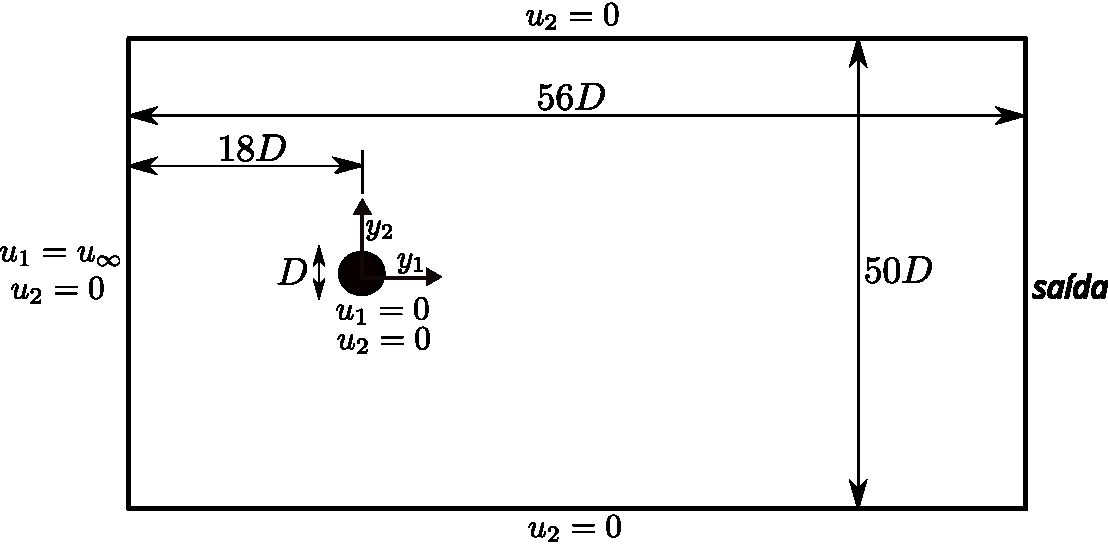
\includegraphics[scale=0.5,trim=0cm 0cm 0cm 0cm, clip=true]{Imagens/Cap2/cilindro_geometria.pdf}}\\
	\subfloat[Discretização espacial\label{fig:cilindro_malha}]{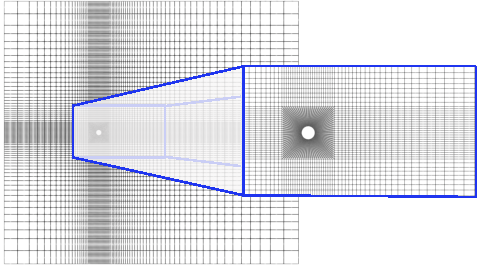
\includegraphics[trim=0cm 2cm 0cm 2cm,clip,scale=0.4]{Imagens/Cap2/cilindro_malha.pdf}}
	\caption{Cilindro: Geometria, condições de contorno e malha de elementos finitos.}
\end{figure}

Para o cálculo dos coeficientes aerodinâmicos é necessário definir-se primeiramente as forças de arrasto - horizontal ($F_D$) e de sustentação - vertical ($F_L$), que são induzidas por tensões desviadores e hidrostáticas e são calculadas pelas seguintes equações:

\begin{align}
F_D = \int_{\boundary_{c}} \stresstensor_{1j}n_{j} \deriv\boundary_{c},
\end{align}

\begin{align}
F_L = \int_{\boundary_{c}} \stresstensor_{2j}n_{j} \deriv\boundary_{c},
\end{align}

\noindent nas quais o símbolo $\boundary_{c}$ representa o contorno do cilindro e $n_j$ é o vetor normal à essa superfície na direção $j$, com $j=1,2$. Os coeficientes de arrasto e sustentação são definidos respectivamente por:

\begin{align}
	C_D = \frac{F_D}{0,5\density \lVert \velocinfty \lVert^{2} L},
\end{align}

\begin{align}
	C_L = \frac{F_L}{0,5\density \lVert \velocinfty \lVert^{2} L},
\end{align}.

Devido ao fenômeno de desprendimento de vórtices que ocorre a partir de determinado número de Reynolds do escoamento, é usual determinar-se a frequência deste fenômeno através do número adimensional de Strouhal ($\Strouhal$), dado por:

\begin{align}
	\Strouhal = \frac{f_{v}L}{\lVert \velocinfty \lVert},
\end{align}.

\noindent com $f_{v}$ sendo a frequência de desprendimento dos vórtices.

Como pode-se observar na Fig. \ref{fig:cilindro_coefAero} para $\Reynolds = 40$, os coeficientes de arrasto e de sustentação, após o escoamento entrar em fase estacionária, se mantém constantes ao longo de todo o tempo de análise. Isso ocorre, visto que para Reynolds entre 5 à 50, aproximadamente, formam-se dois vórtices simétricos e estacionários na região logo após o cilindro. Posteriormente, o par de vórtices se quebra e passa existir a chamada esteira de Von Karmán, que ocorre devido à formação de vórtices de maneira alternada entre as regiões superior e inferior do cilindro, o que pode ser notado também na Fig. \ref{fig:cilindro_coefAero}  para $\Reynolds = 100$ e $\Reynolds=1000$. Os valores do coeficiente de Strouhal, para $Re = 100$ e $Re=1000$, foram de 0,1665 e 0,2381 respectivamente. Os valores obtidos para os coeficientes aerodinâmicos foram os esperados para o problema em questão (ver, por exemplo, \citeonline{Tonon:2016,Henderson:1997}).

\begin{figure}[!htb]
	\centering
	\subfloat[\label{fig:cilindro_Cd}Coeficiente de arrasto $ C_D$]{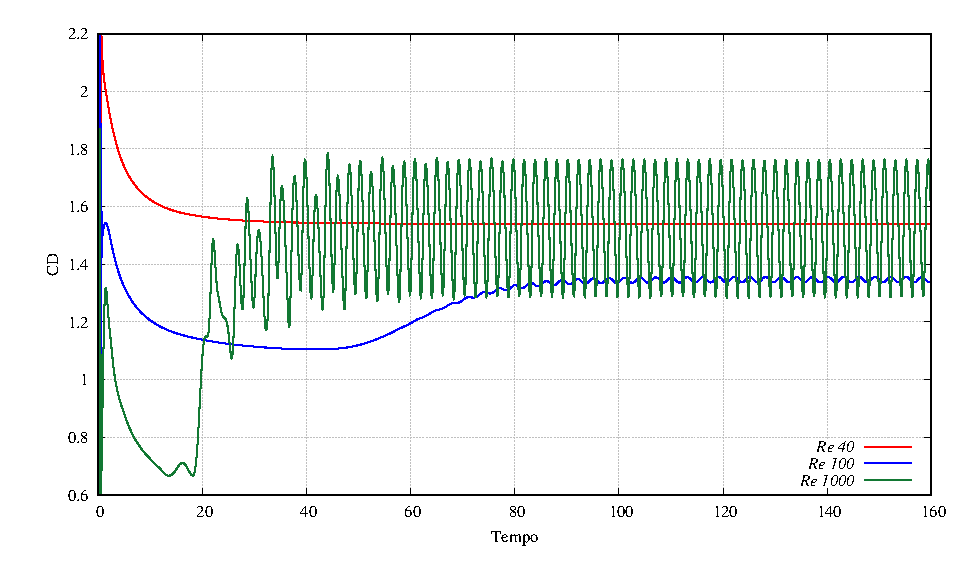
\includegraphics[scale=0.7,trim=0cm 0cm 0cm 0cm, clip=true]{Imagens/Cap2/cilindro_CD.eps}}\\ 
	\subfloat[\label{fig:cilindro_Cl}Coeficiente de sustentação $C_L$]{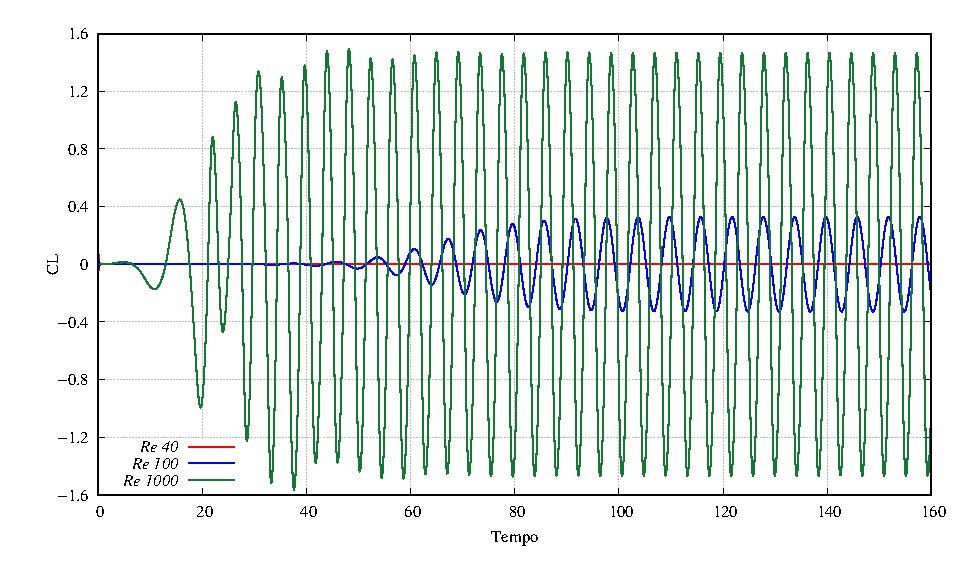
\includegraphics[scale=0.7,trim=0cm 0cm 0cm 0cm, clip=true]{Imagens/Cap2/cilindro_CL.eps}}\\ 
	\caption{Cilindro: Coeficientes aerodinâmicos. }
	\label{fig:cilindro_coefAero}
\end{figure}

Nas Fig. \ref{fig:cilindro_camposVel} e Fig. \ref{fig:cilindro_camposPressao} podem ser observados os campos de velocidade e pressão ao longo de um ciclo de desprendimento de vórtices para $\Reynolds = 100$. Pode-se notar nessas imagens, a formação e o desprendimento de vórtices na esteira de Von Karmán.


\begin{figure}[htb!]
	\centering
	\subfloat[$T_n$]{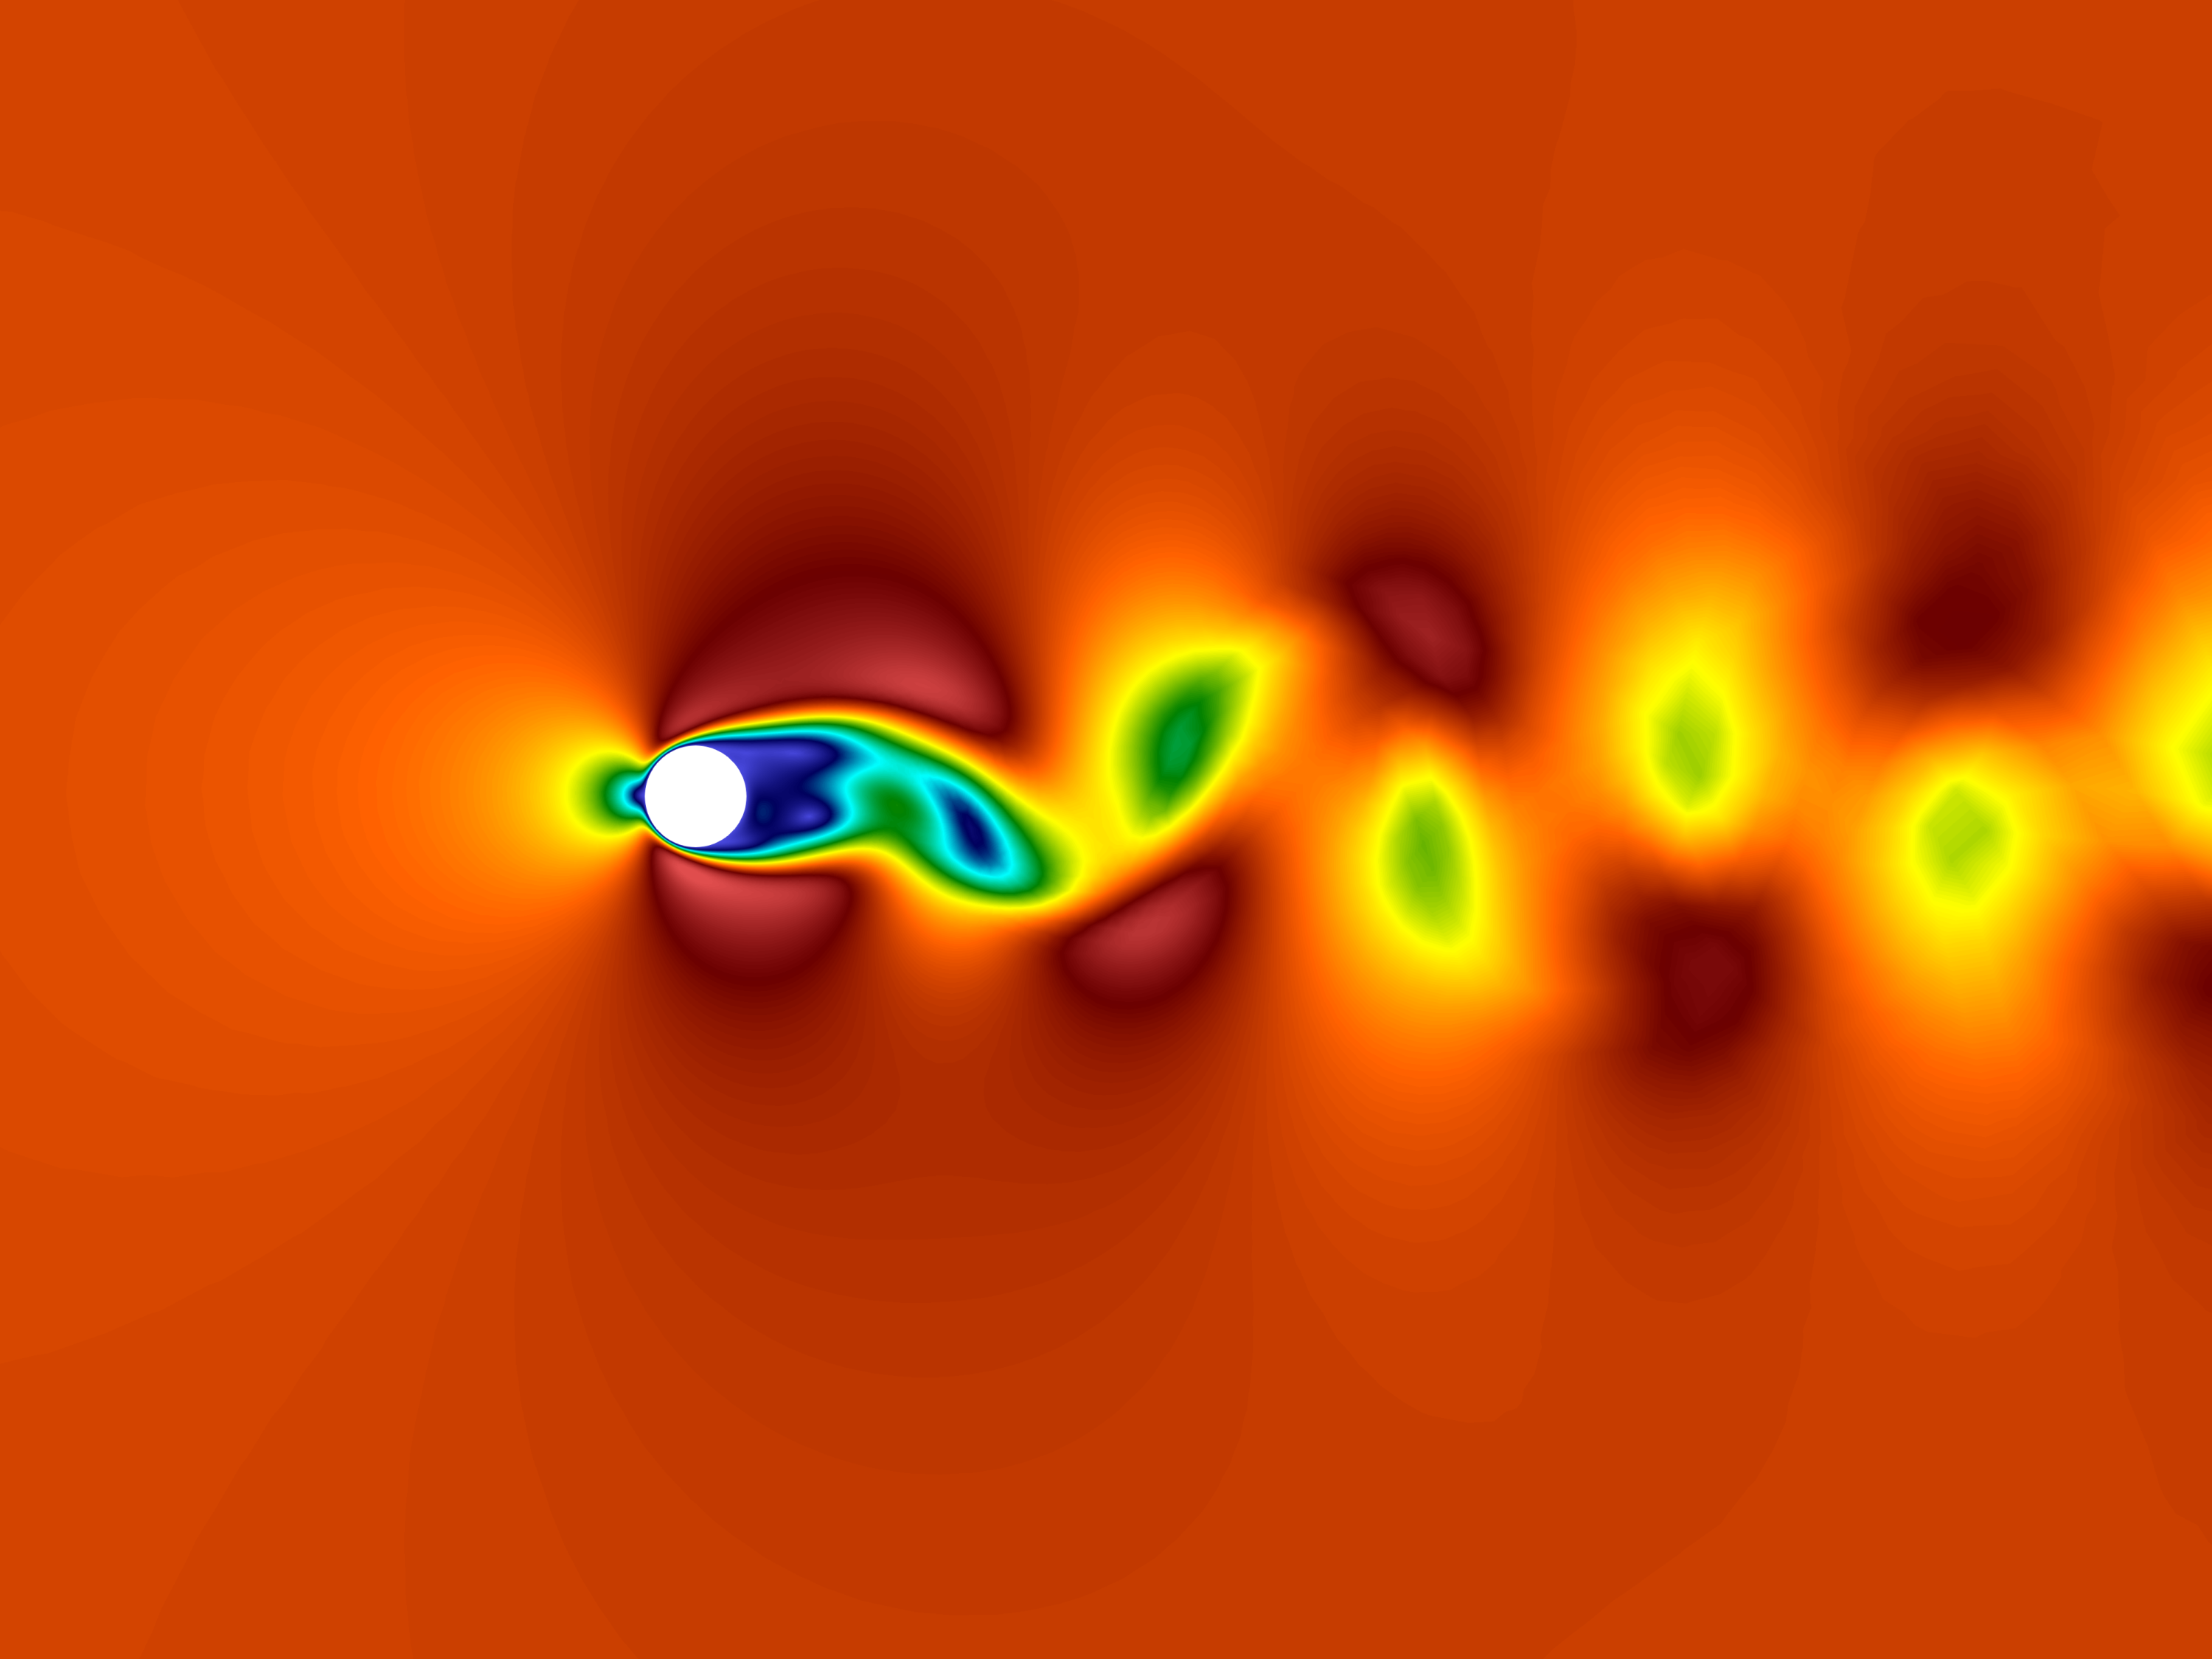
\includegraphics[scale=0.15,trim=5cm 5cm 5cm 6cm, clip=true]{Imagens/Cap2/cilindro_vel2020.pdf}} \
	\subfloat[$T_n + T_n/6$]{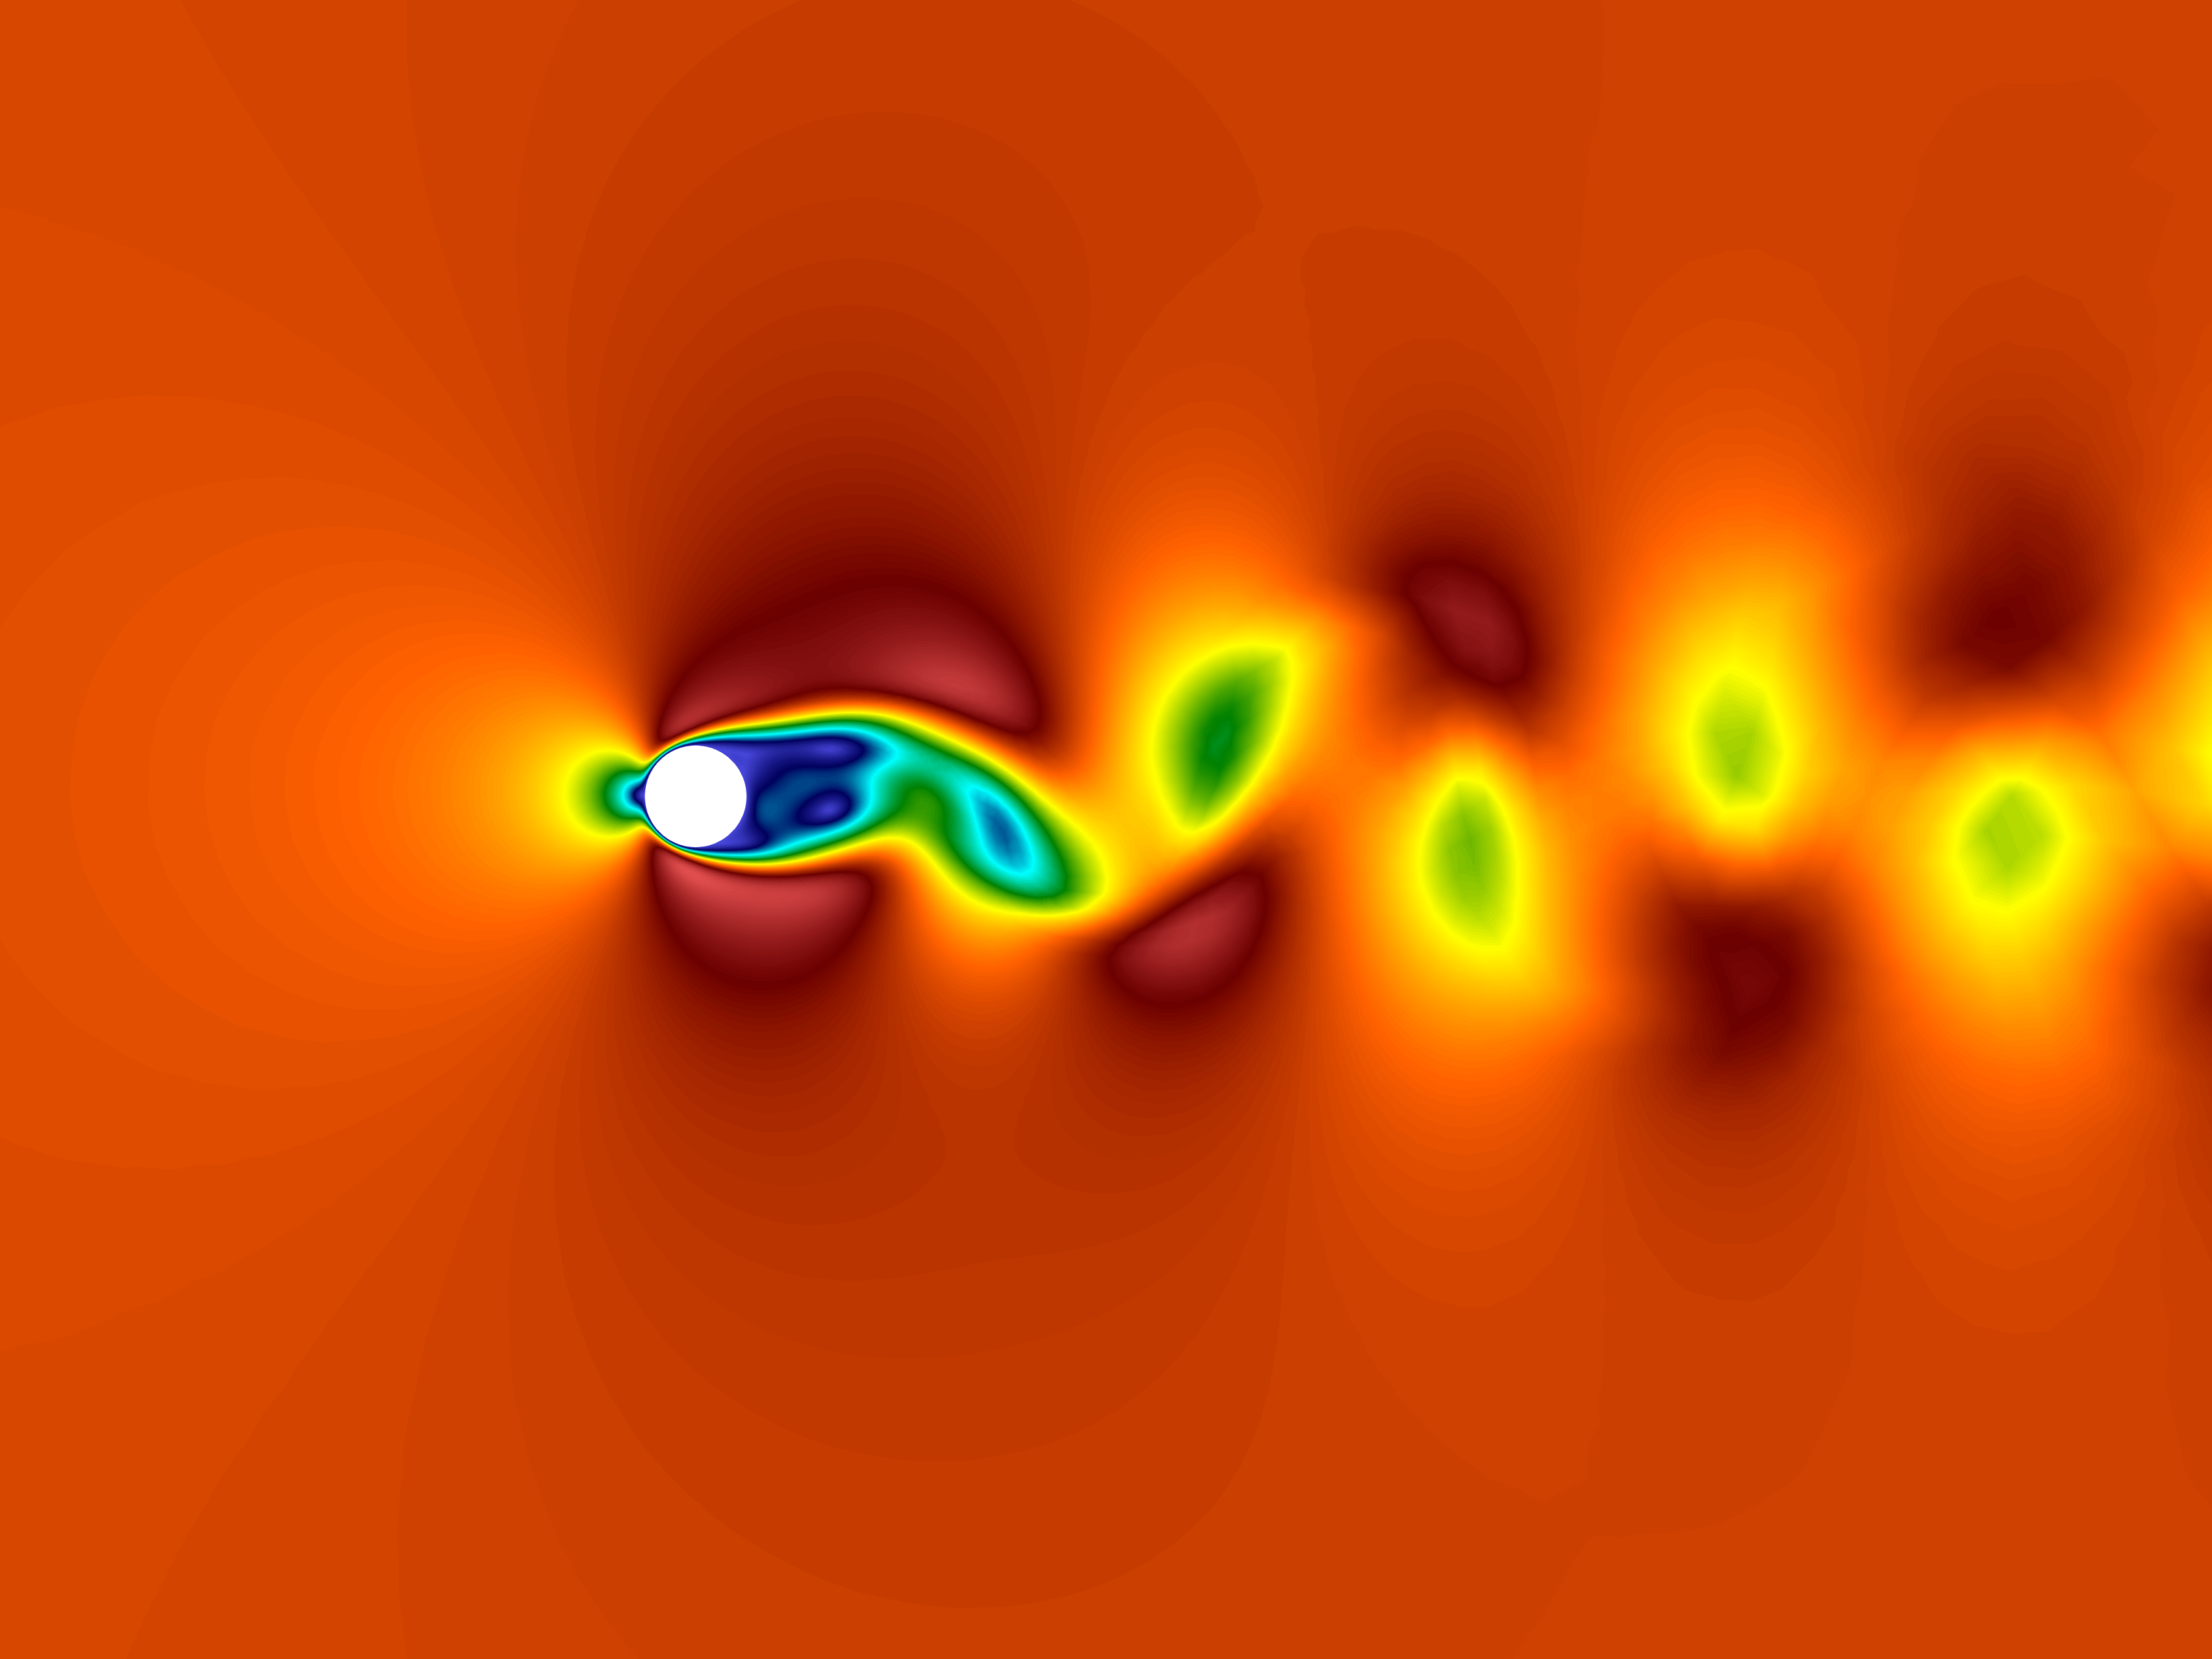
\includegraphics[scale=0.15,trim=5cm 5cm 5cm 6cm, clip=true]{Imagens/Cap2/cilindro_vel2030.pdf}} \\
	\subfloat[$T_n + T_n/3$]{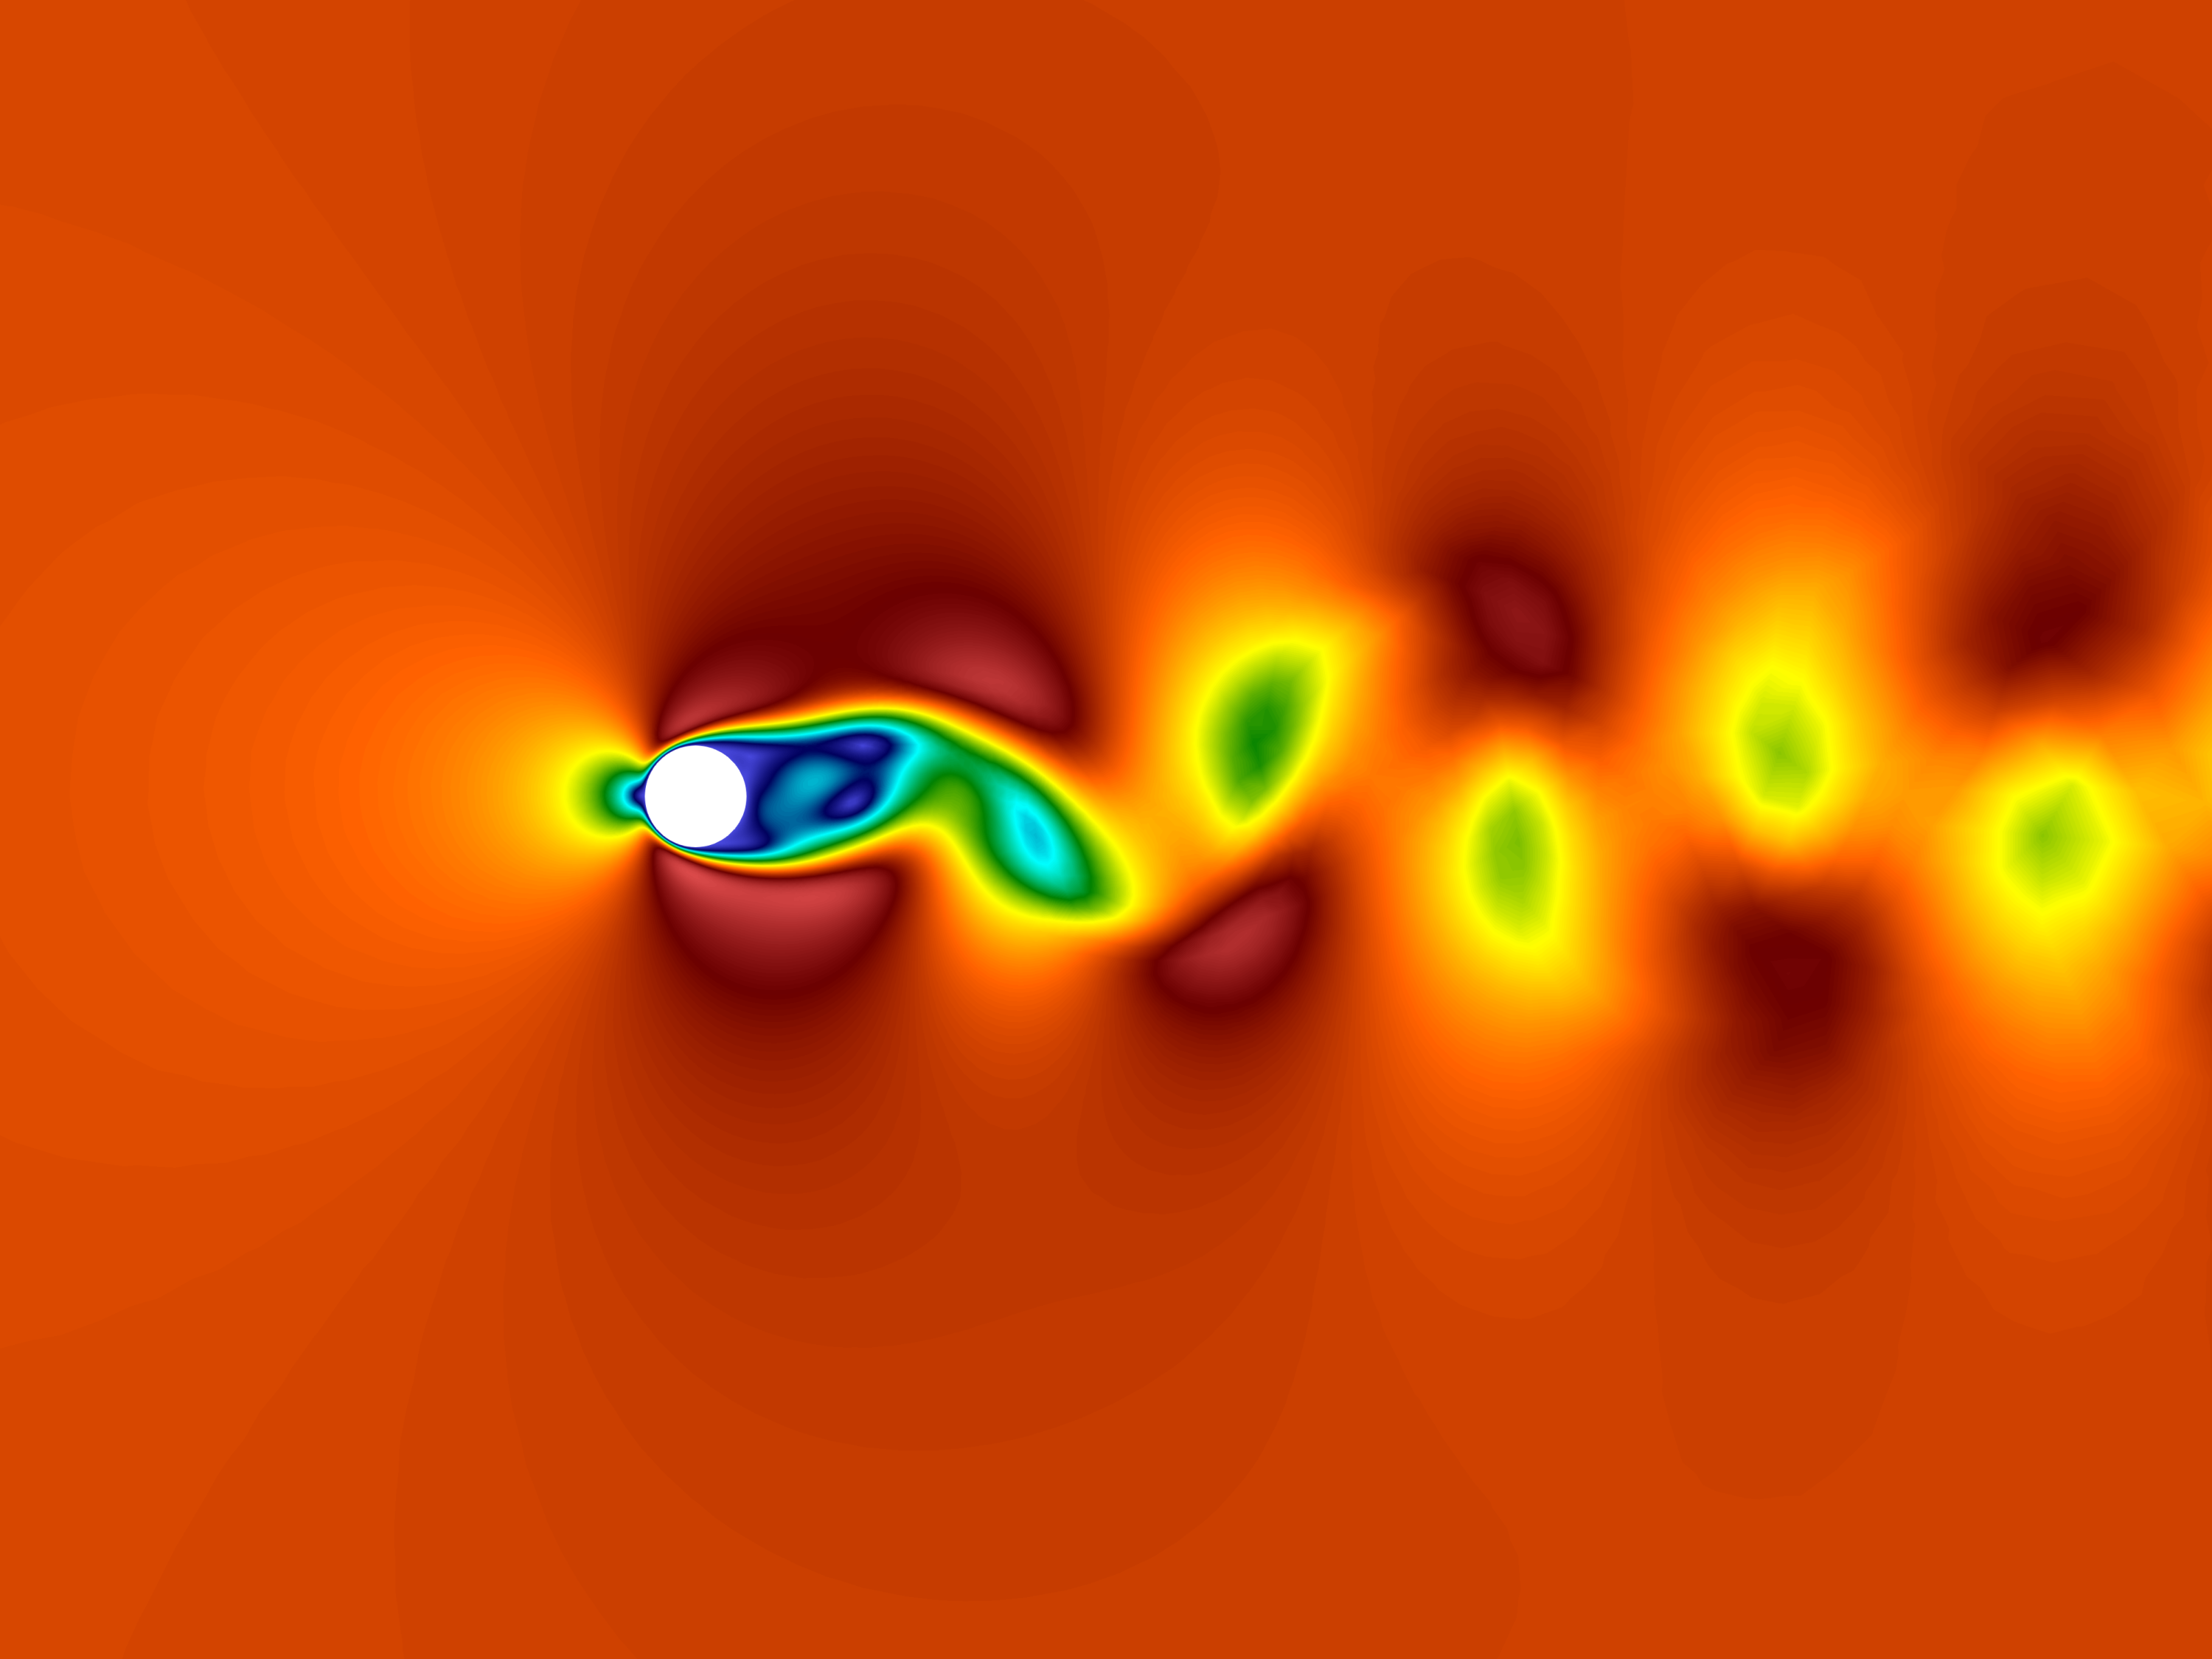
\includegraphics[scale=0.15,trim=5cm 5cm 5cm 6cm, clip=true]{Imagens/Cap2/cilindro_vel2040.pdf}} \
	\subfloat[$T_n + T_n/2$]{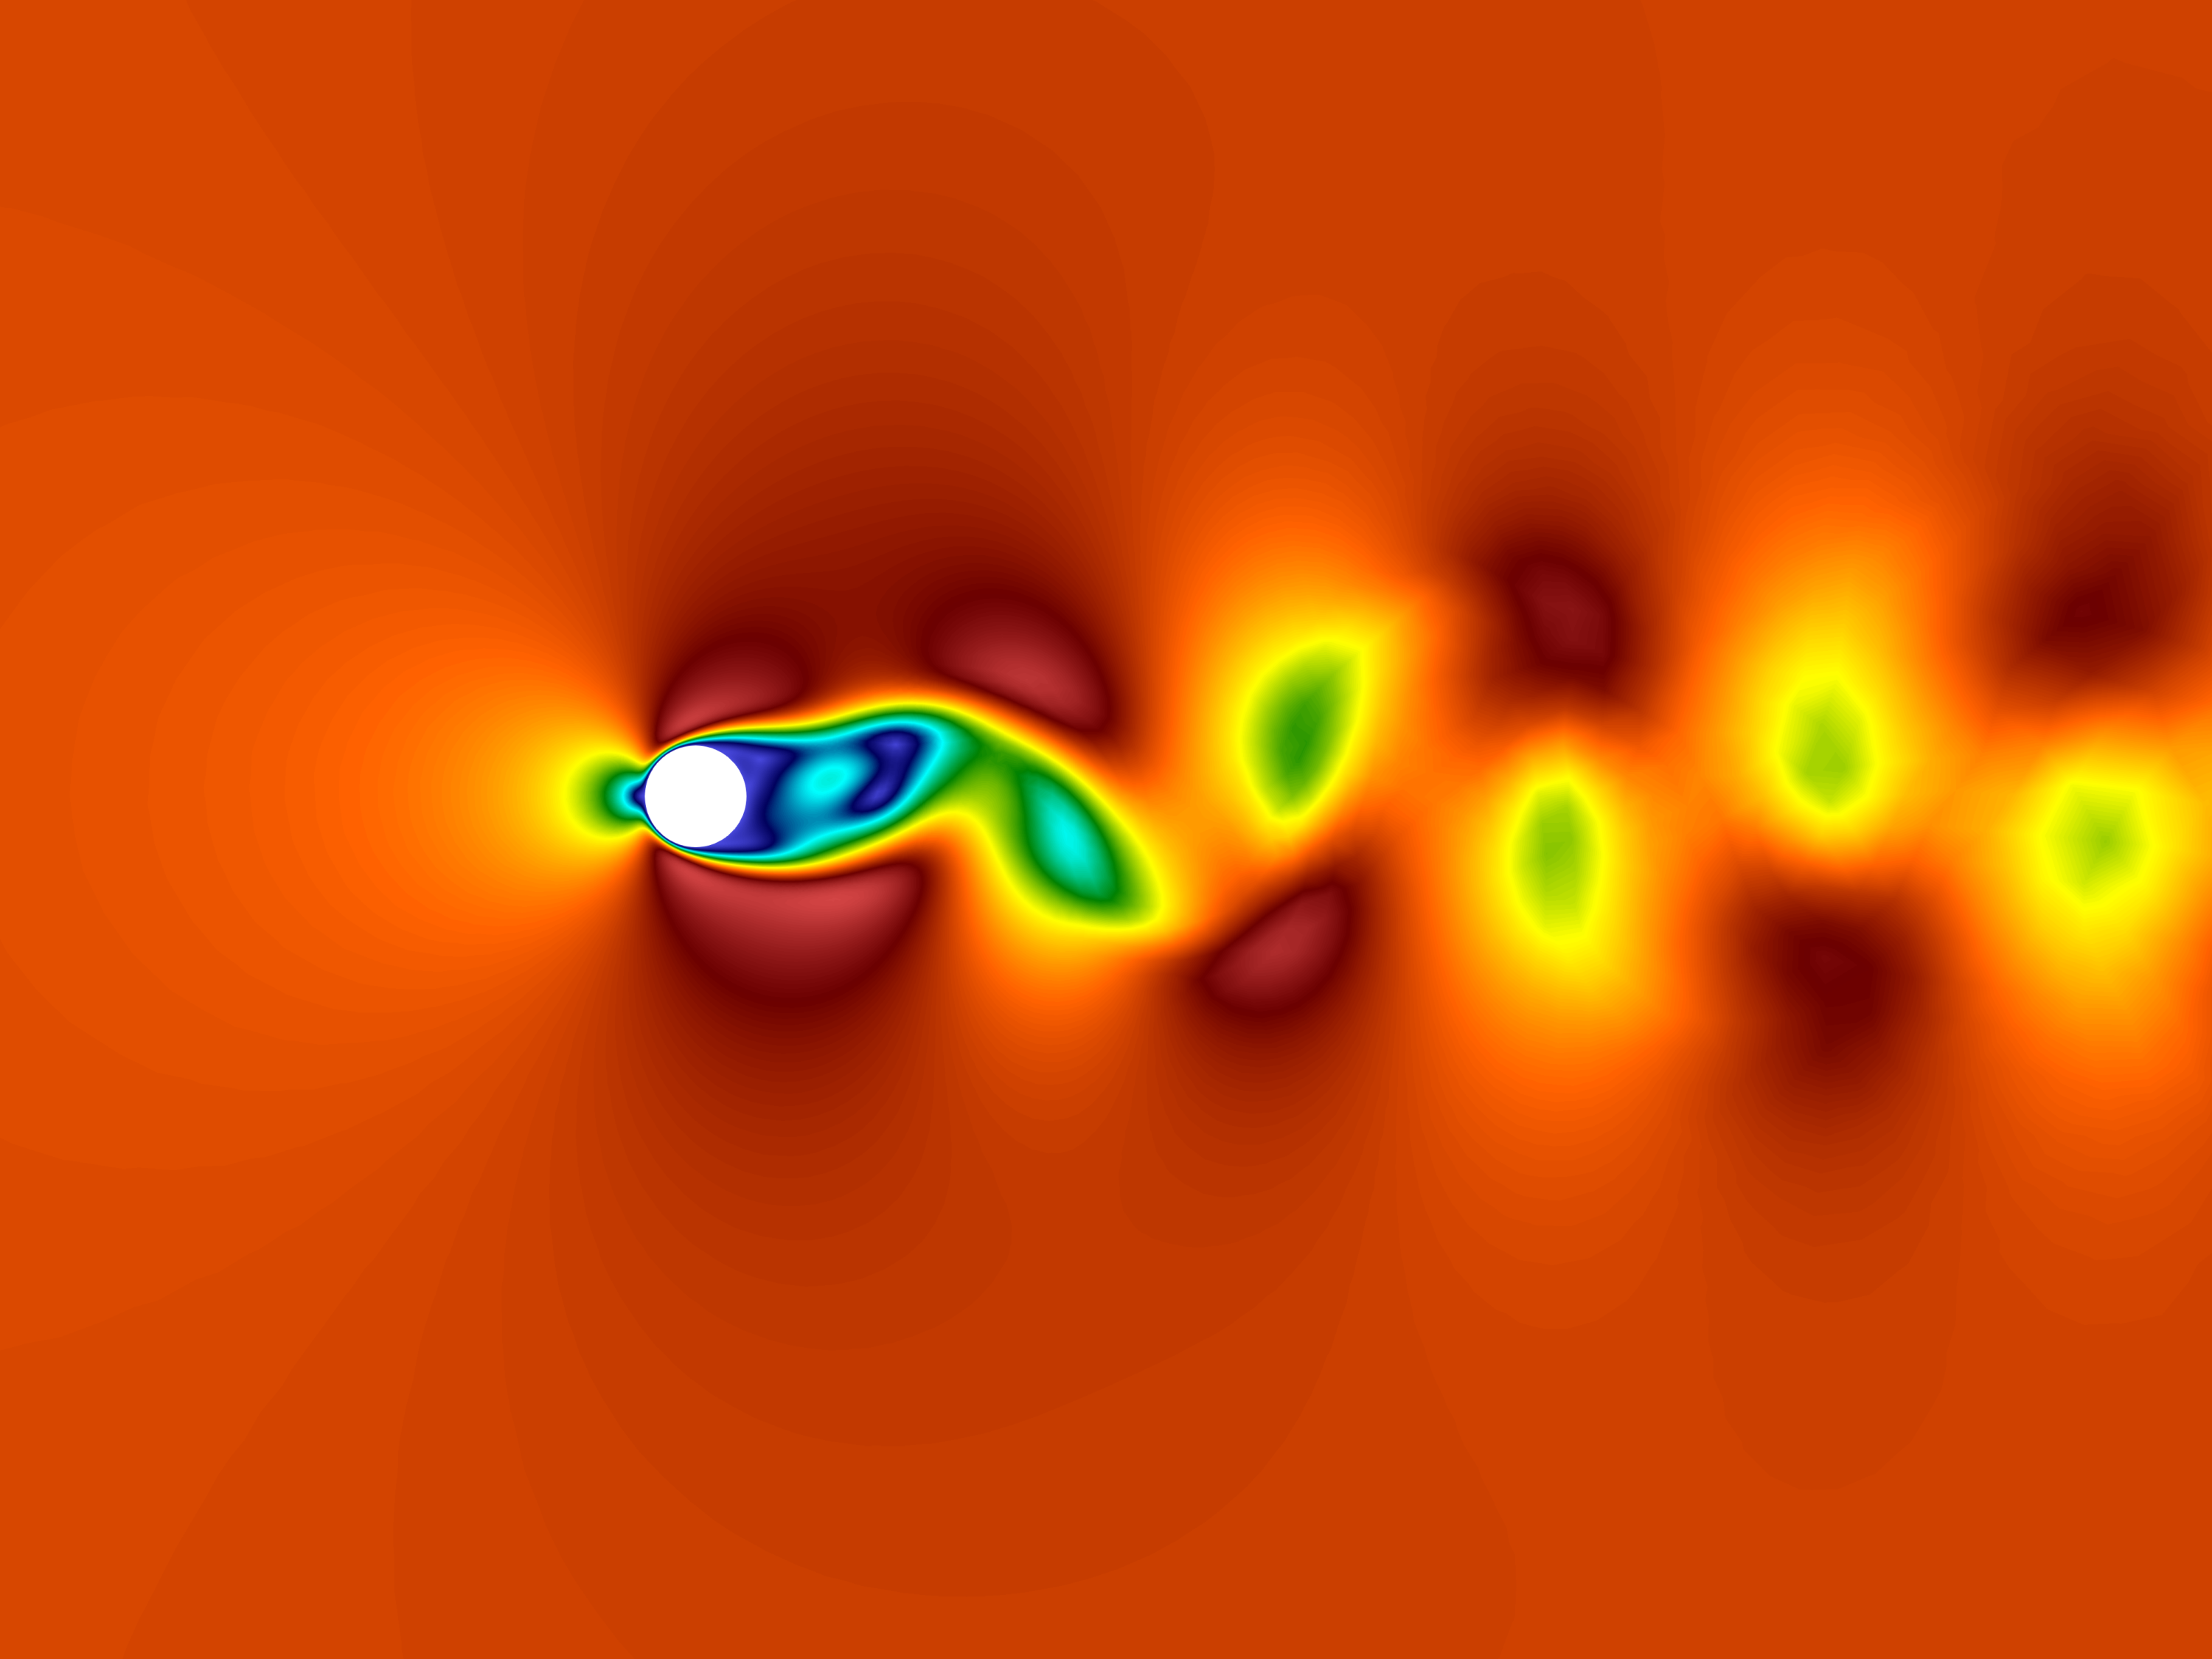
\includegraphics[scale=0.15,trim=5cm 5cm 5cm 6cm, clip=true]{Imagens/Cap2/cilindro_vel2050.pdf}} \\
	\subfloat[$T_n + 2T_n/3$]{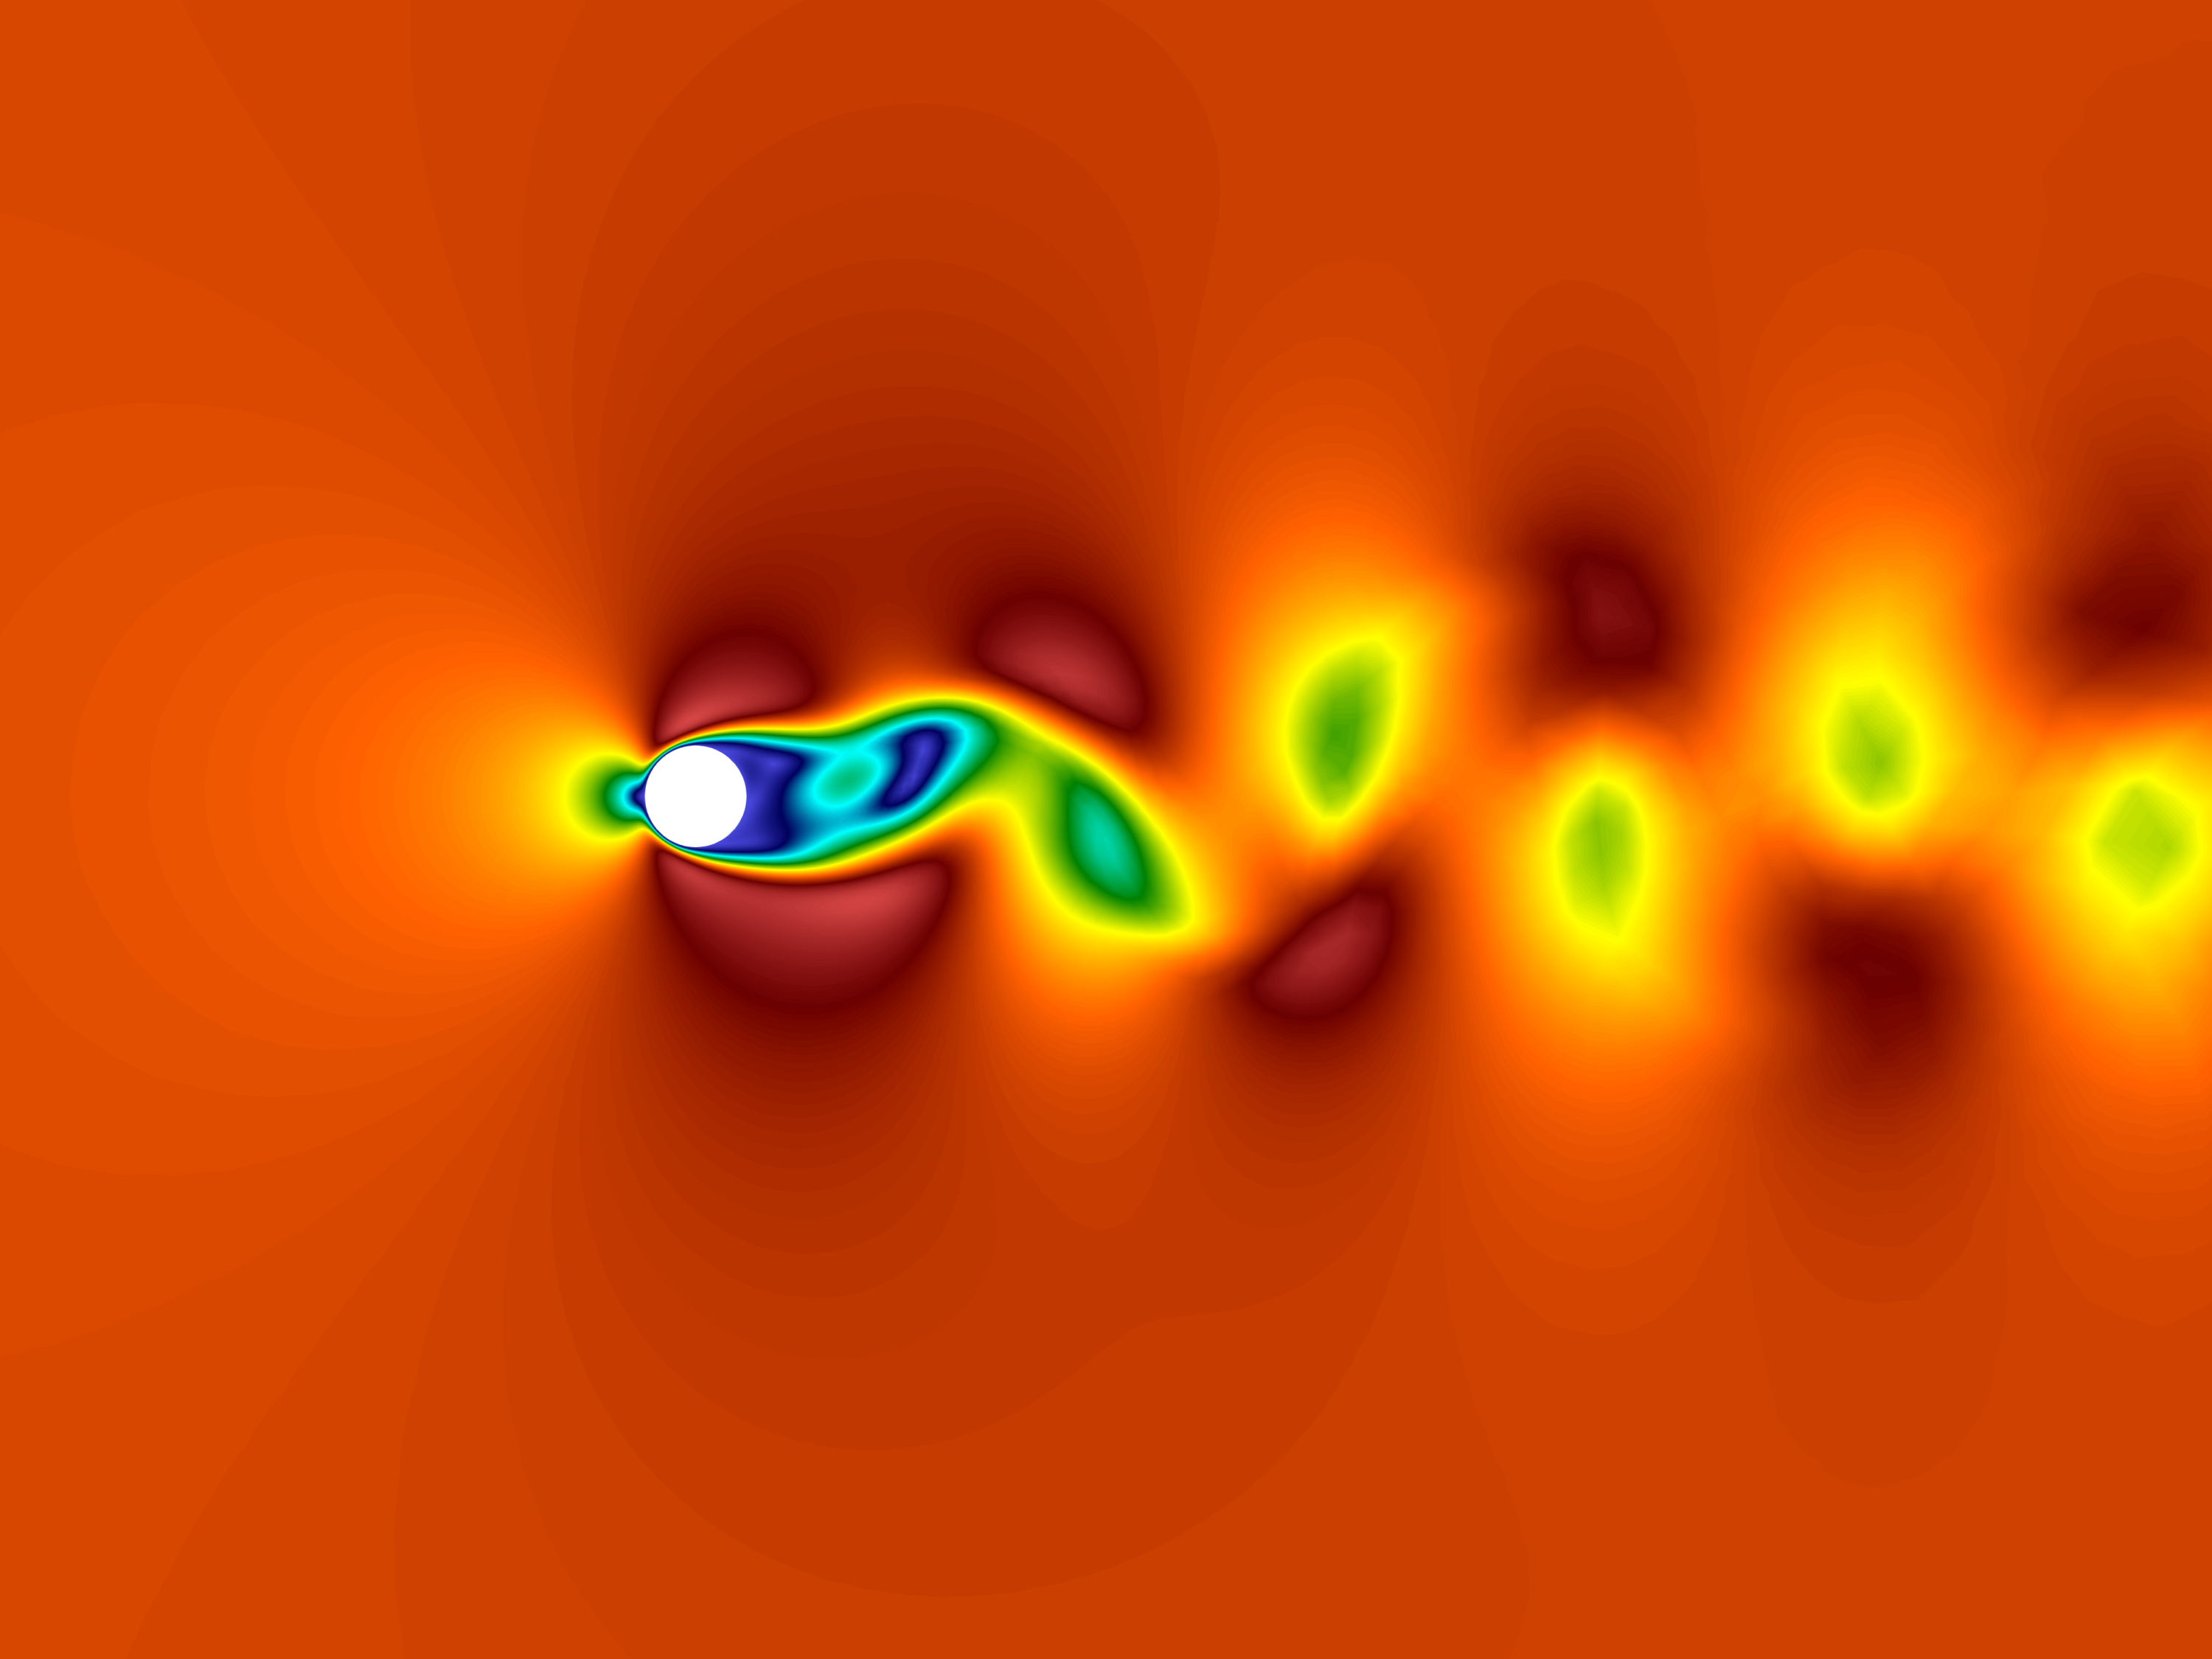
\includegraphics[scale=0.15,trim=5cm 5cm 5cm 6cm, clip=true]{Imagens/Cap2/cilindro_vel2060.pdf}} \
	\subfloat[$T_n + 5T_n/6$]{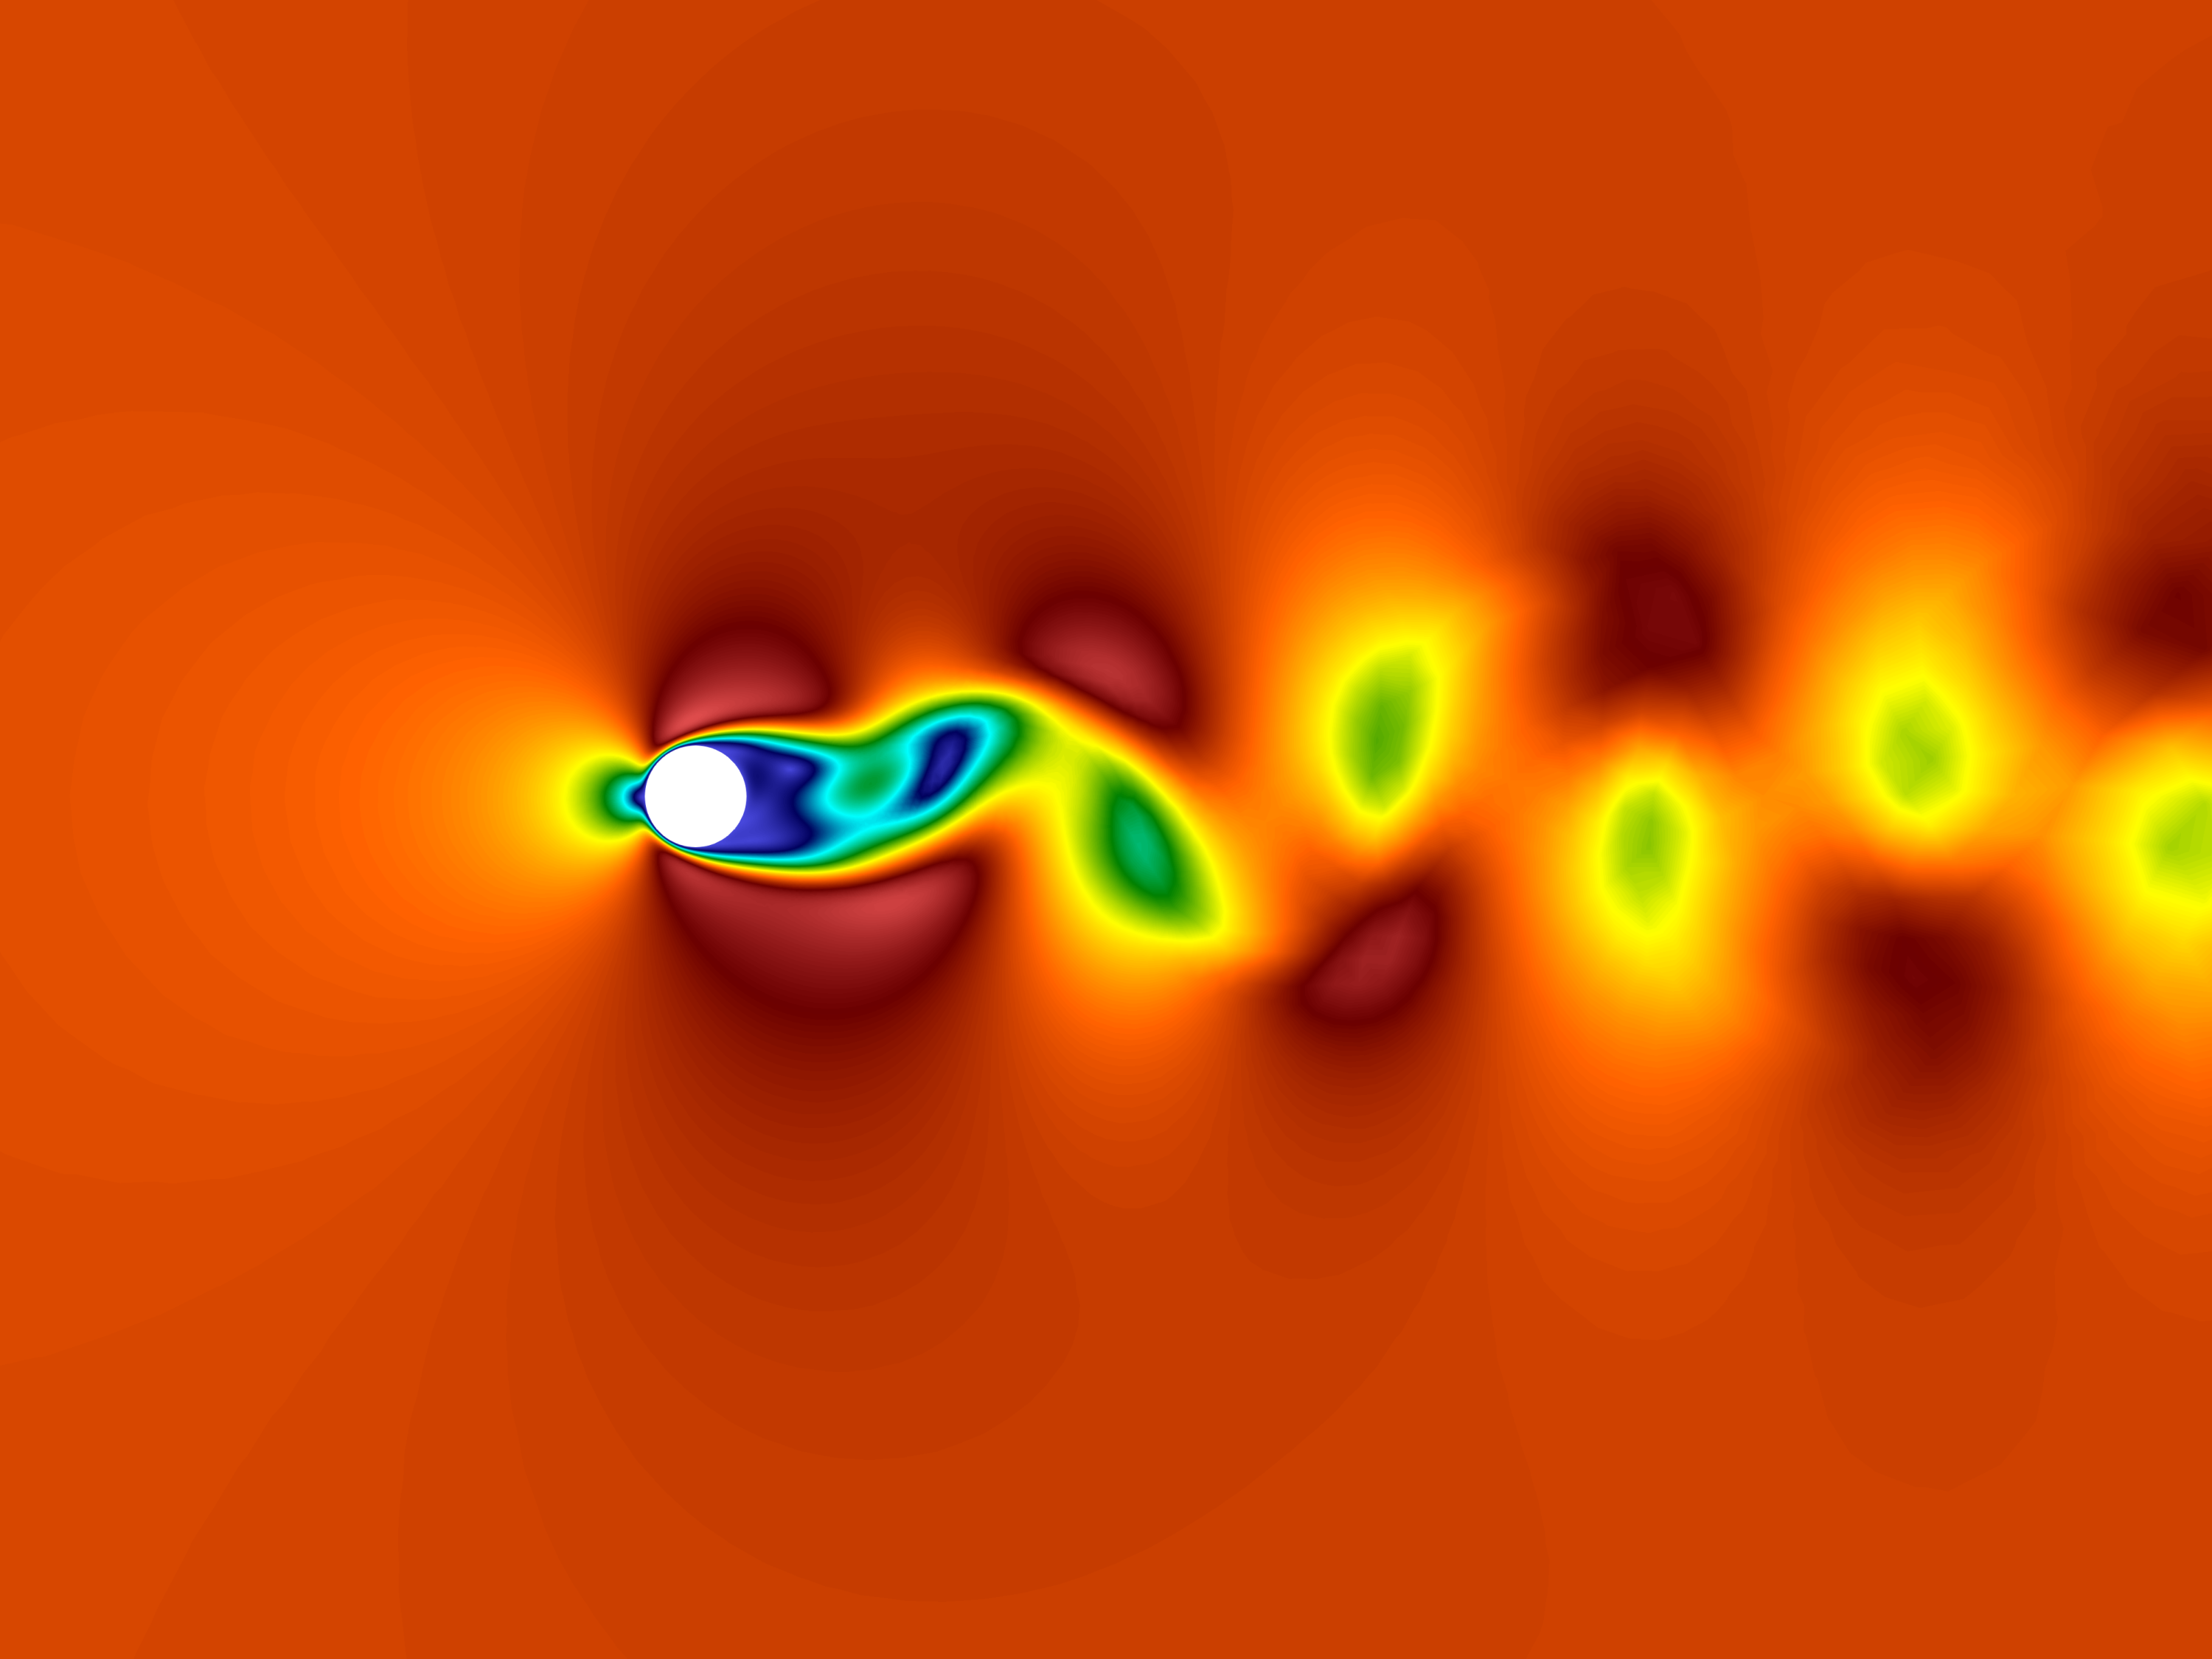
\includegraphics[scale=0.15,trim=5cm 5cm 5cm 6cm, clip=true]{Imagens/Cap2/cilindro_vel2070.pdf}} \\
	{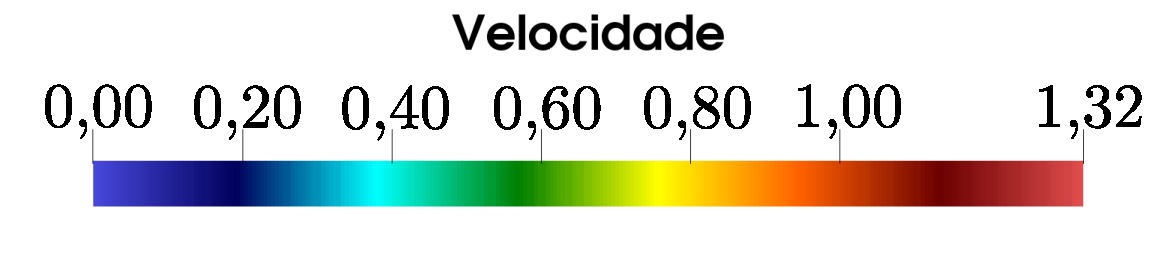
\includegraphics[trim=0cm 0cm 0cm 0cm,clip=true,scale=0.3]{Imagens/Cap2/cilindro_legendaVel.pdf}} \\
	\caption{Cilindro: Campos de velocidade}
	\label{fig:cilindro_camposVel}
\end{figure}

\begin{figure}[htb!]
	\centering
	\subfloat[$T_n$]{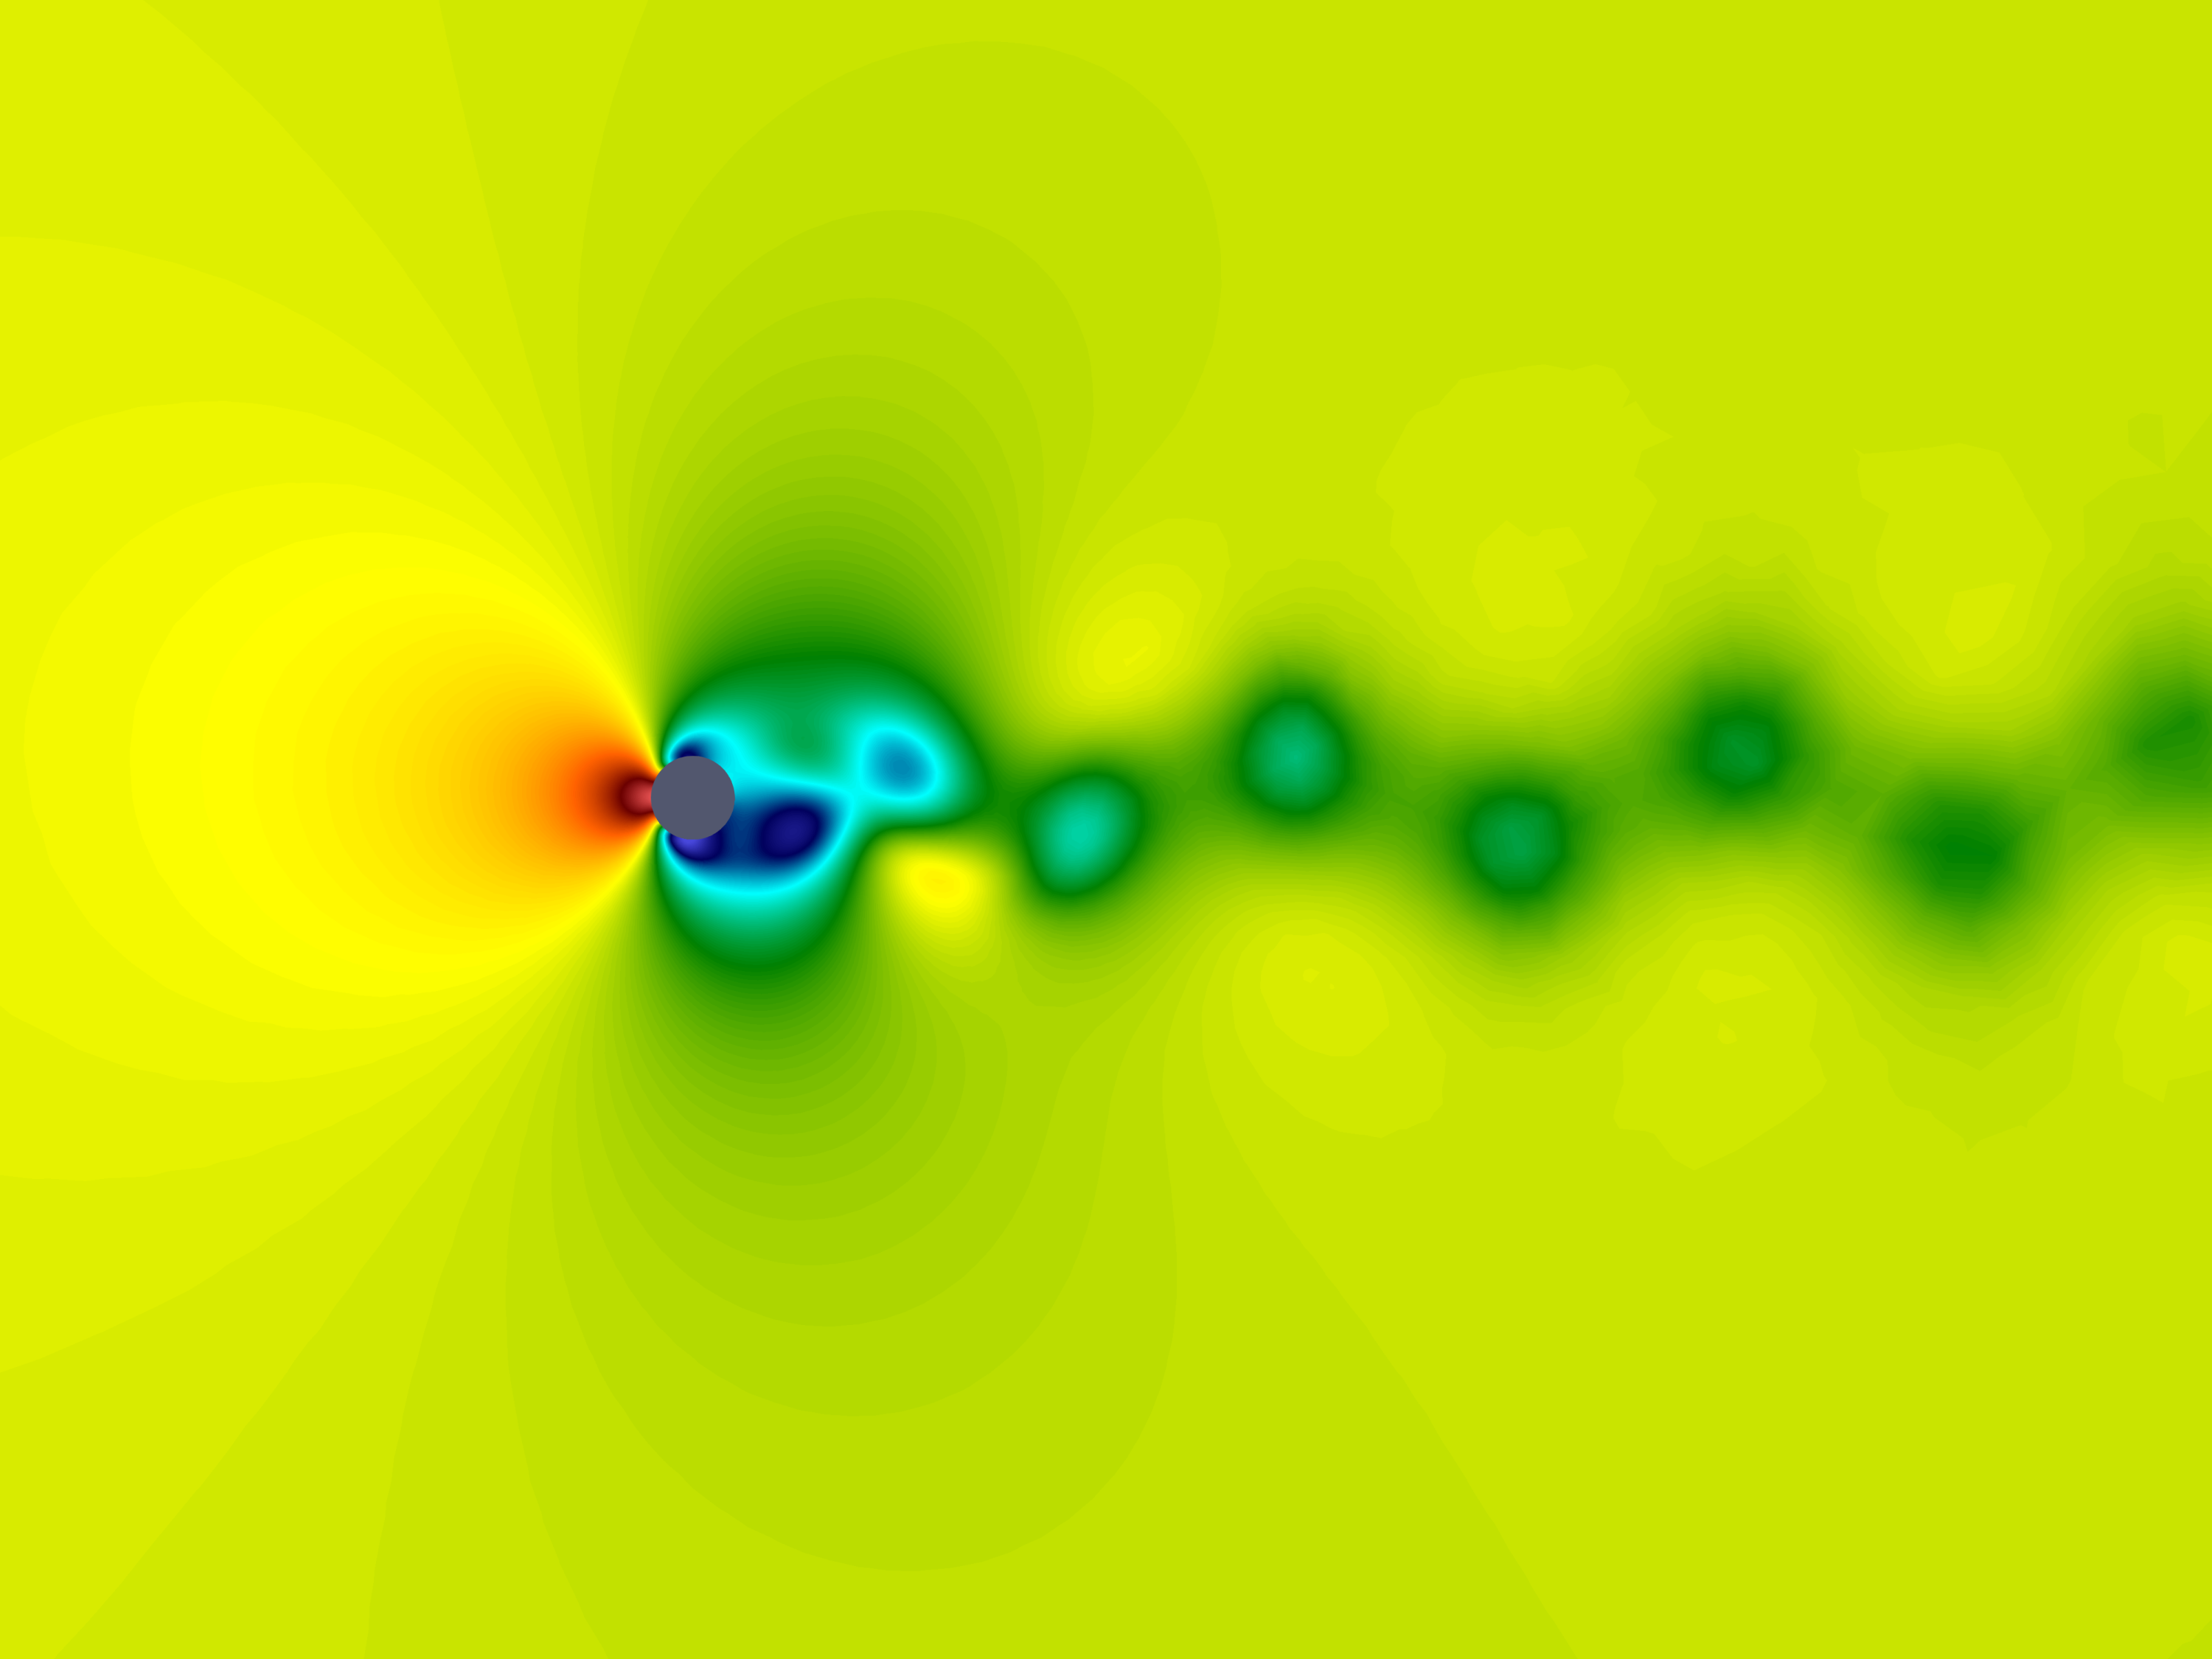
\includegraphics[scale=0.15,trim=5cm 5cm 5cm 6cm, clip=true]{Imagens/Cap2/cilindro_press2020.pdf}} \
	\subfloat[$T_n + T_n/6$]{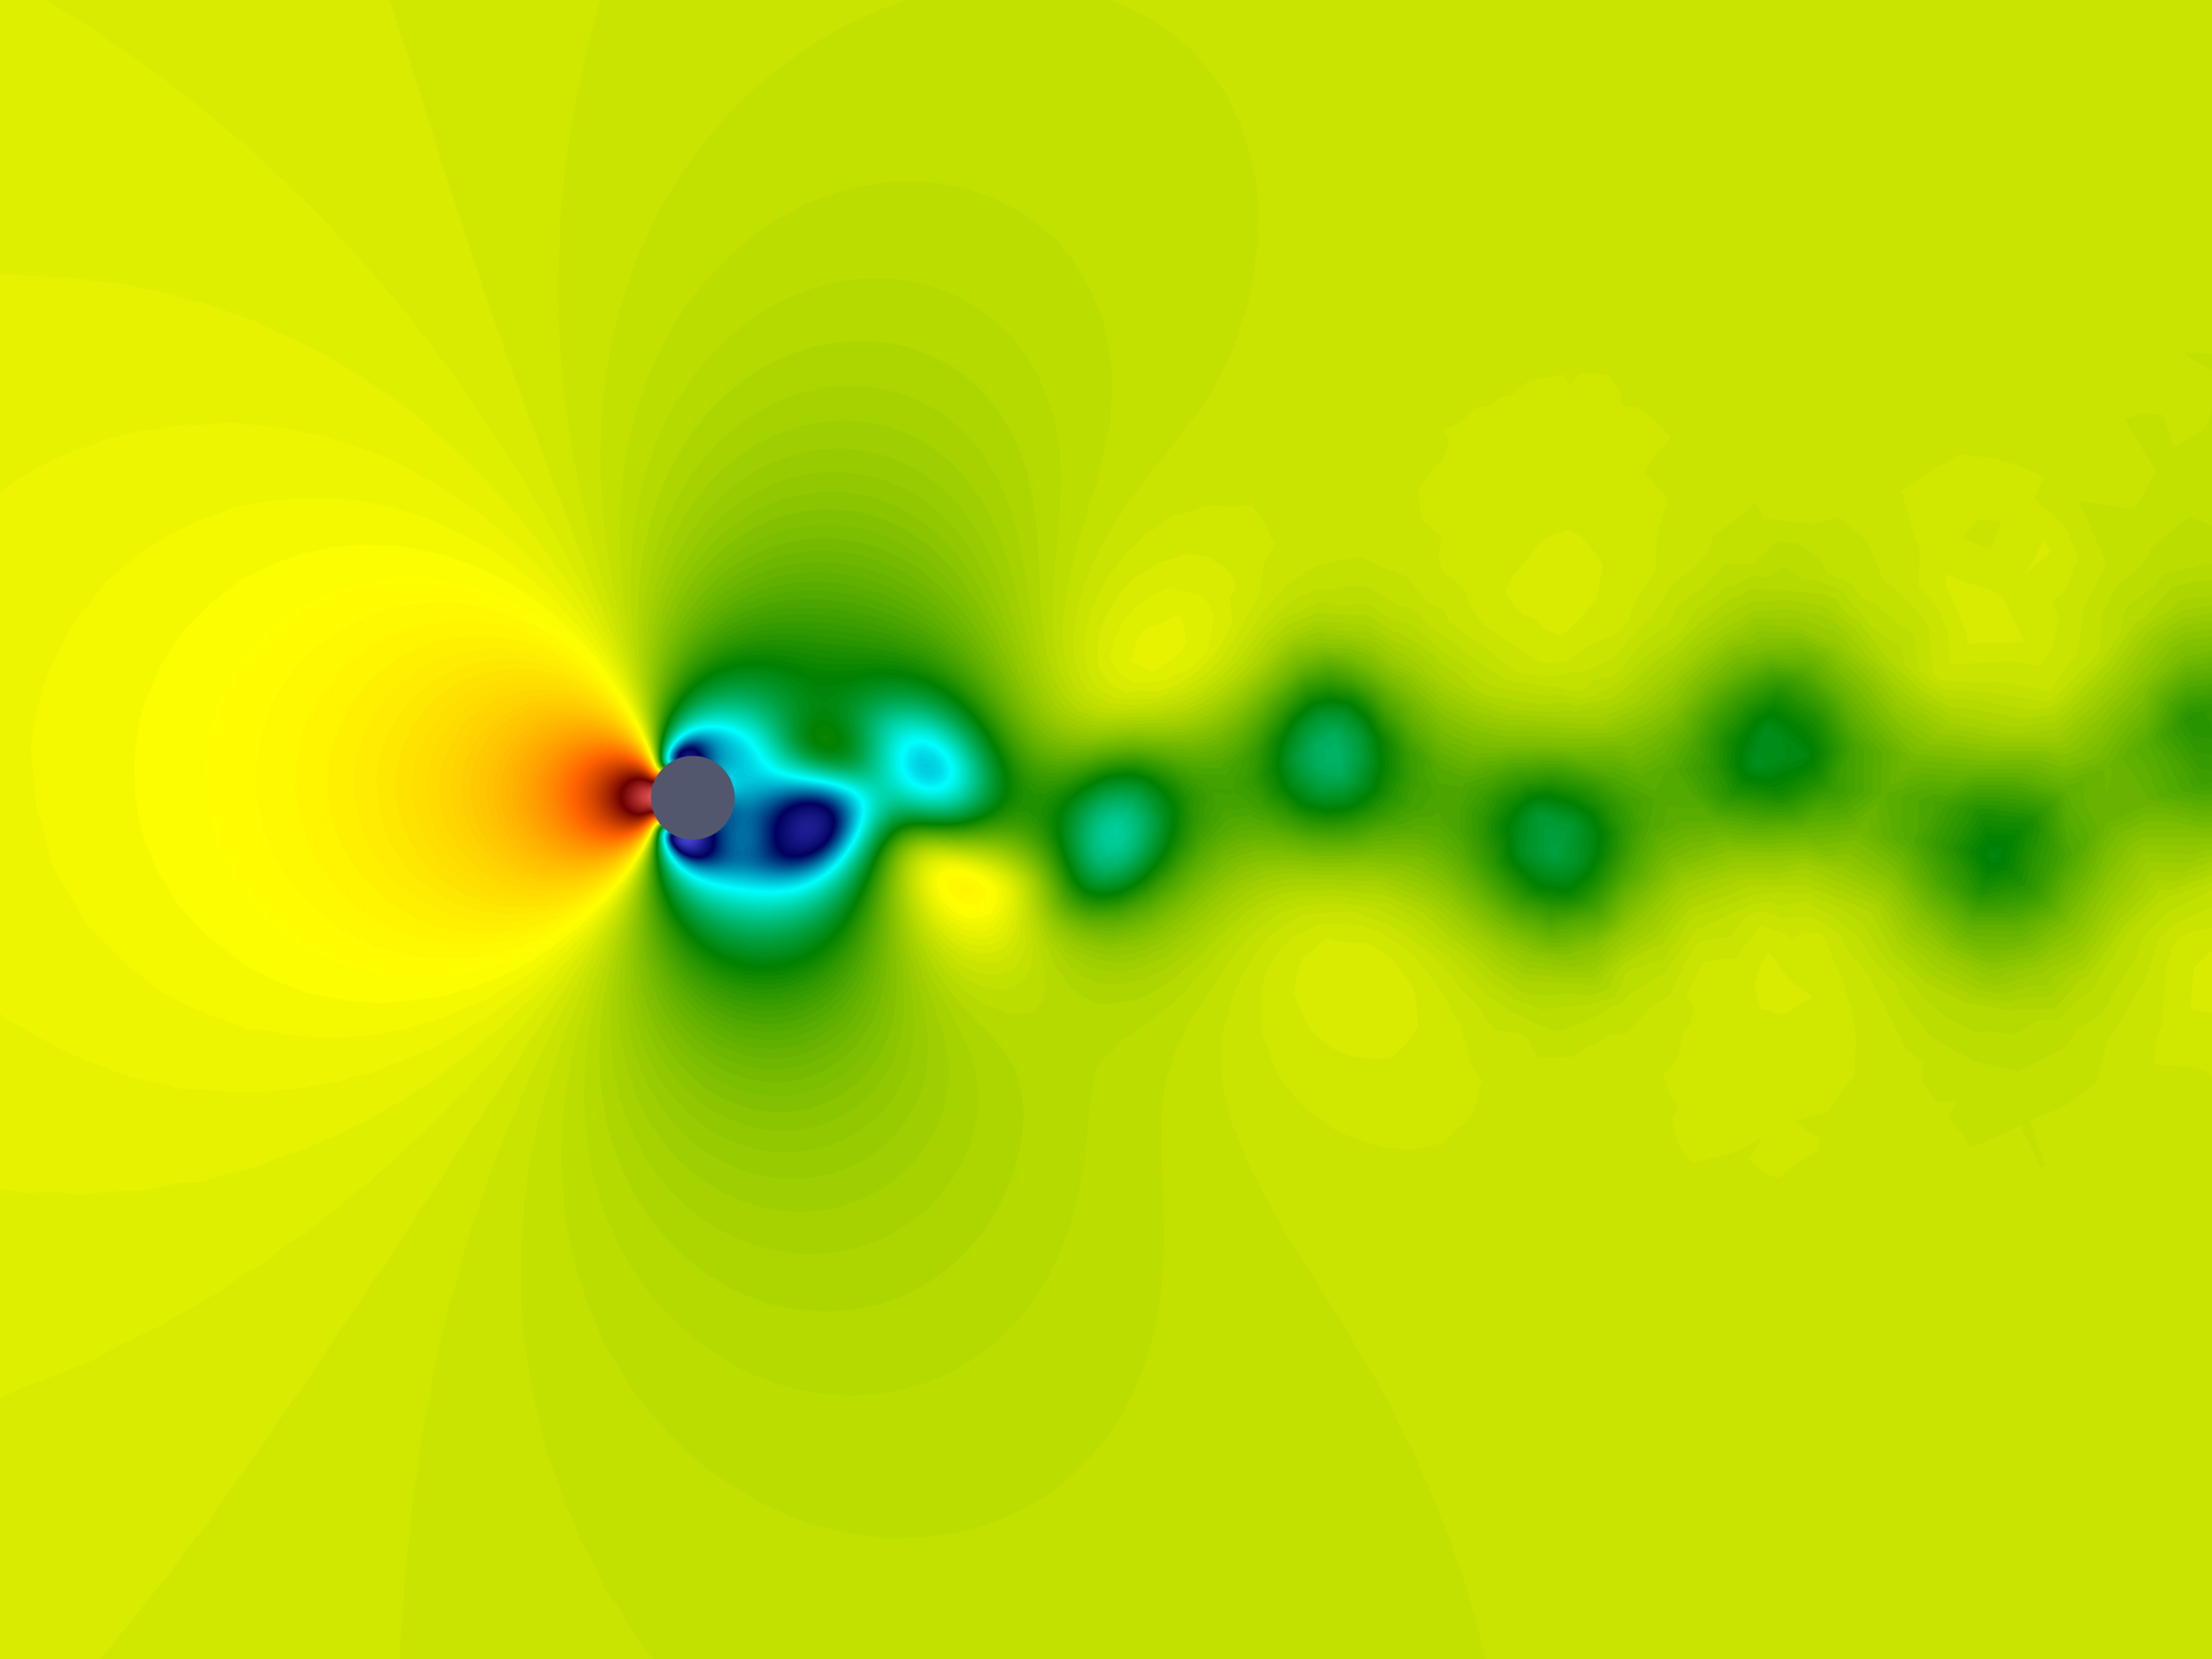
\includegraphics[scale=0.15,trim=5cm 5cm 5cm 6cm, clip=true]{Imagens/Cap2/cilindro_press2030.pdf}} \\
	\subfloat[$T_n + T_n/3$]{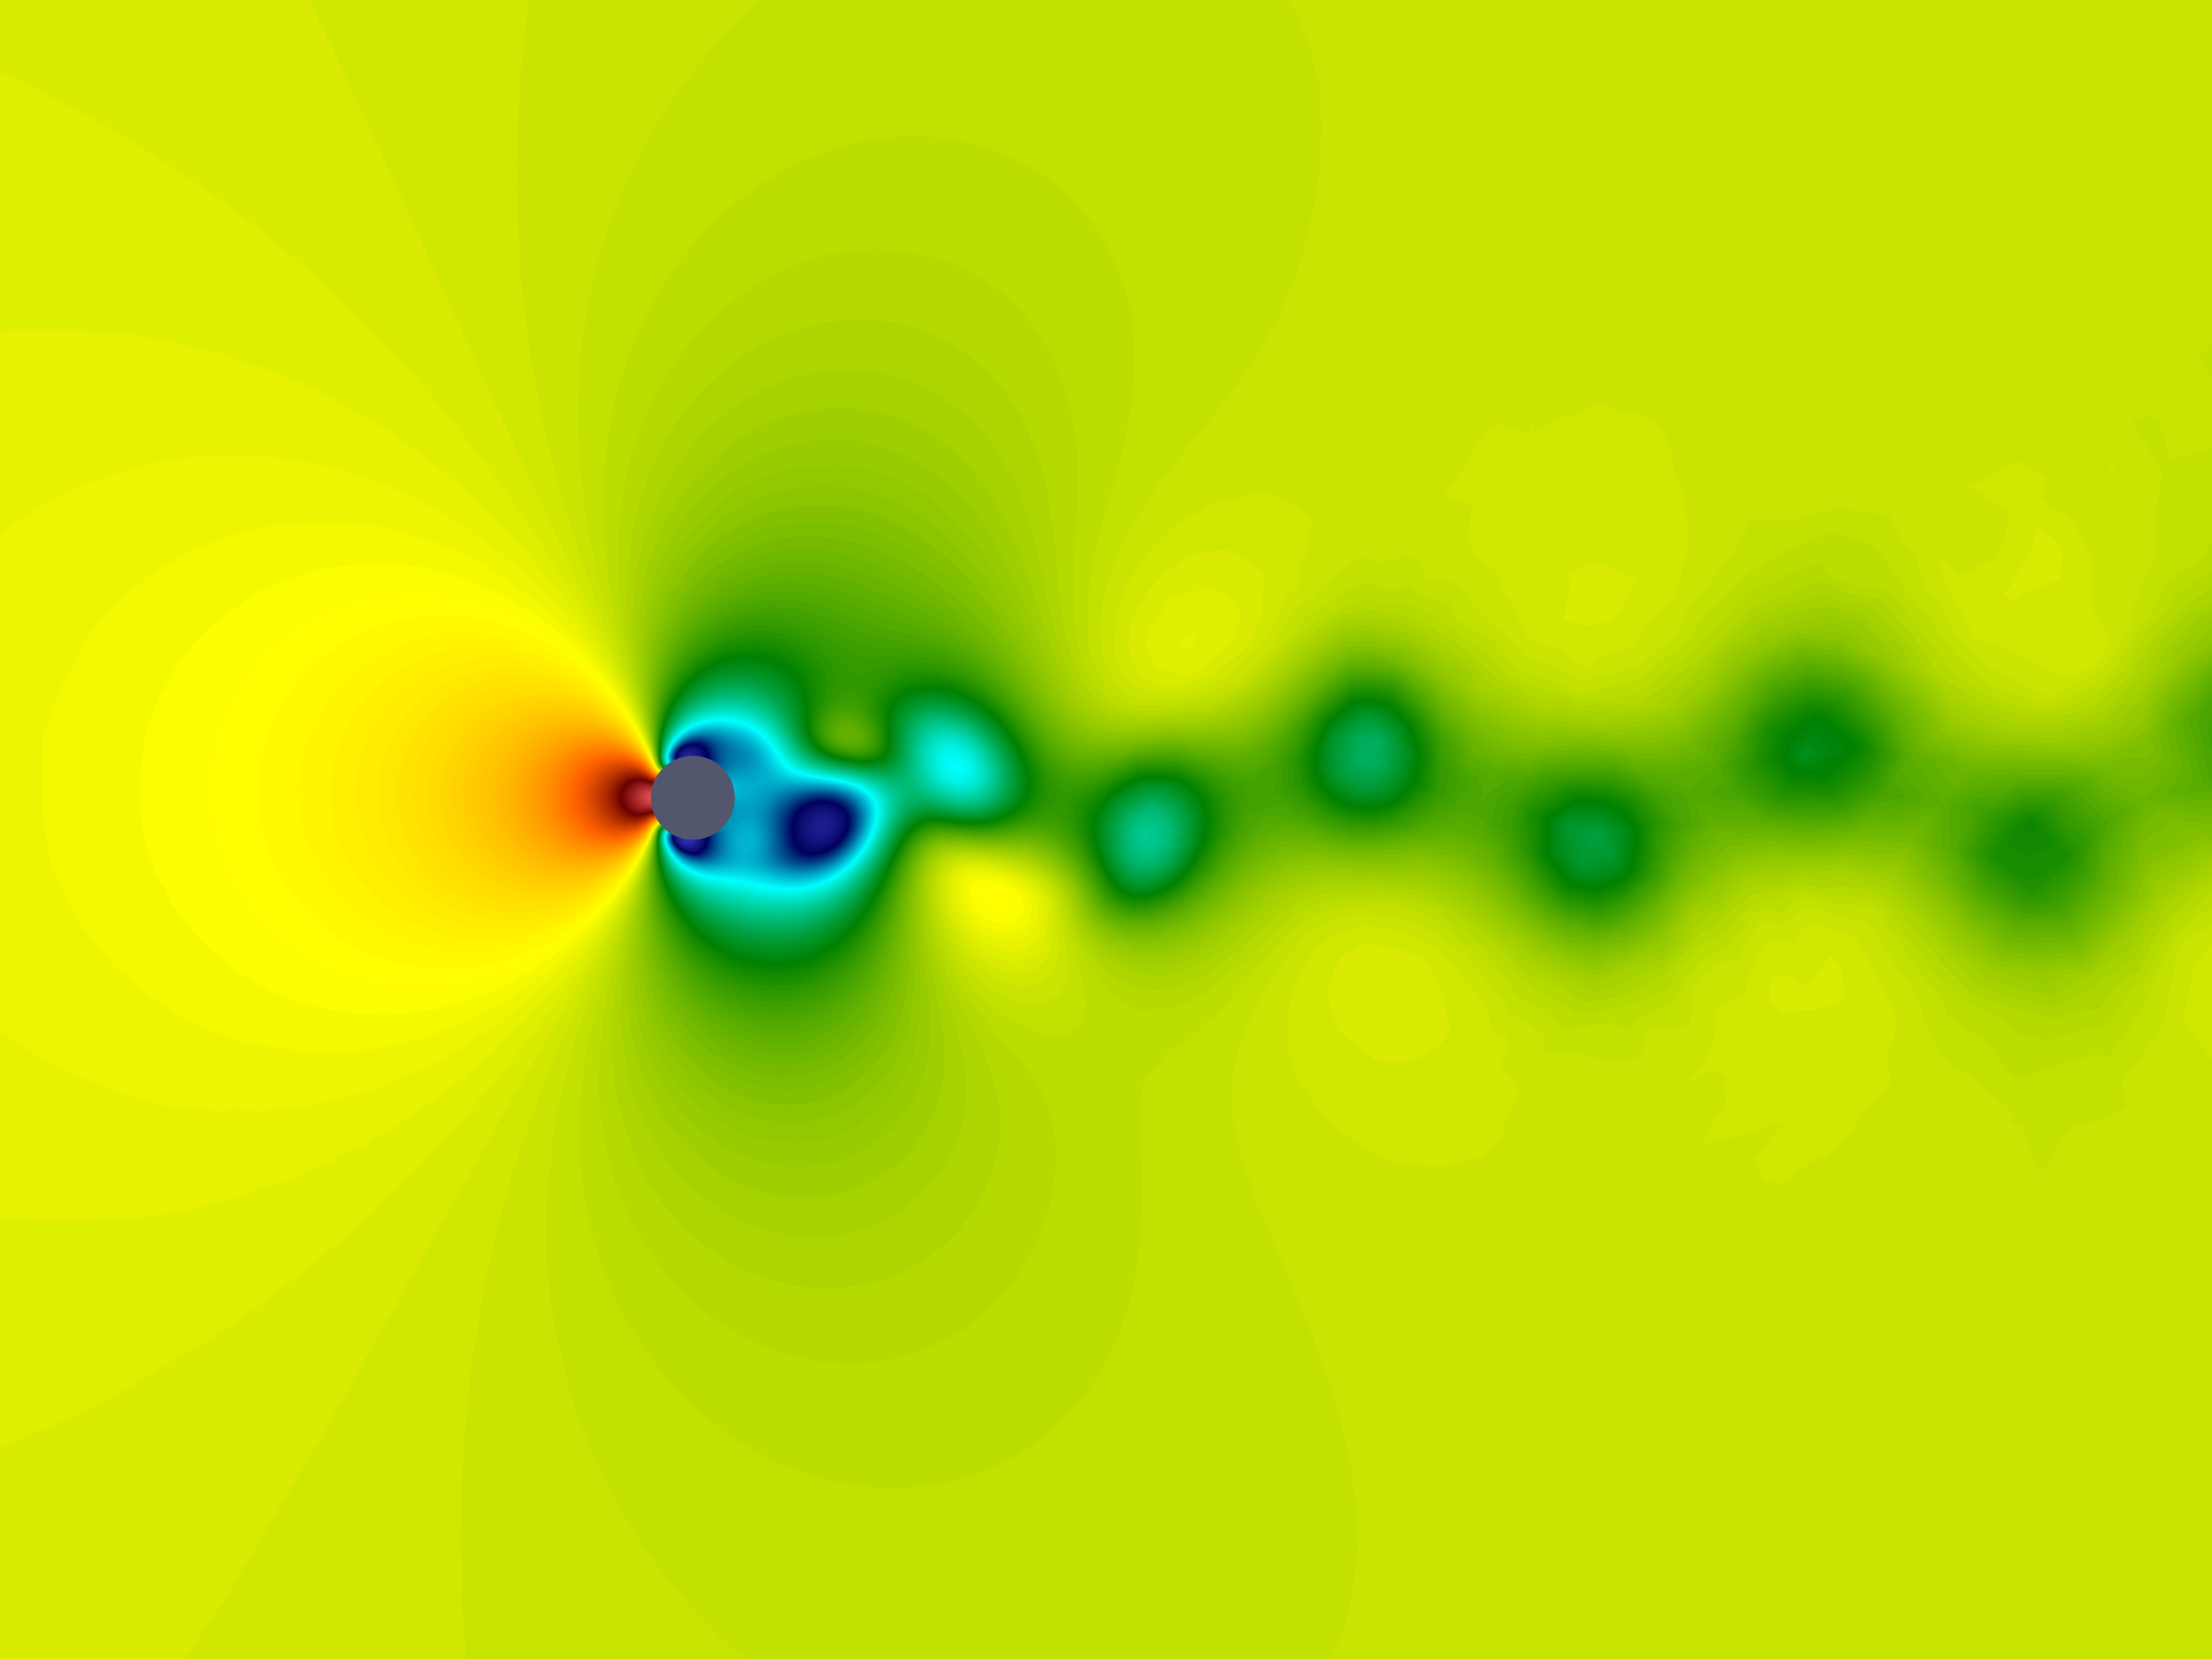
\includegraphics[scale=0.15,trim=5cm 5cm 5cm 6cm, clip=true]{Imagens/Cap2/cilindro_press2040.pdf}} \
	\subfloat[$T_n + T_n/2$]{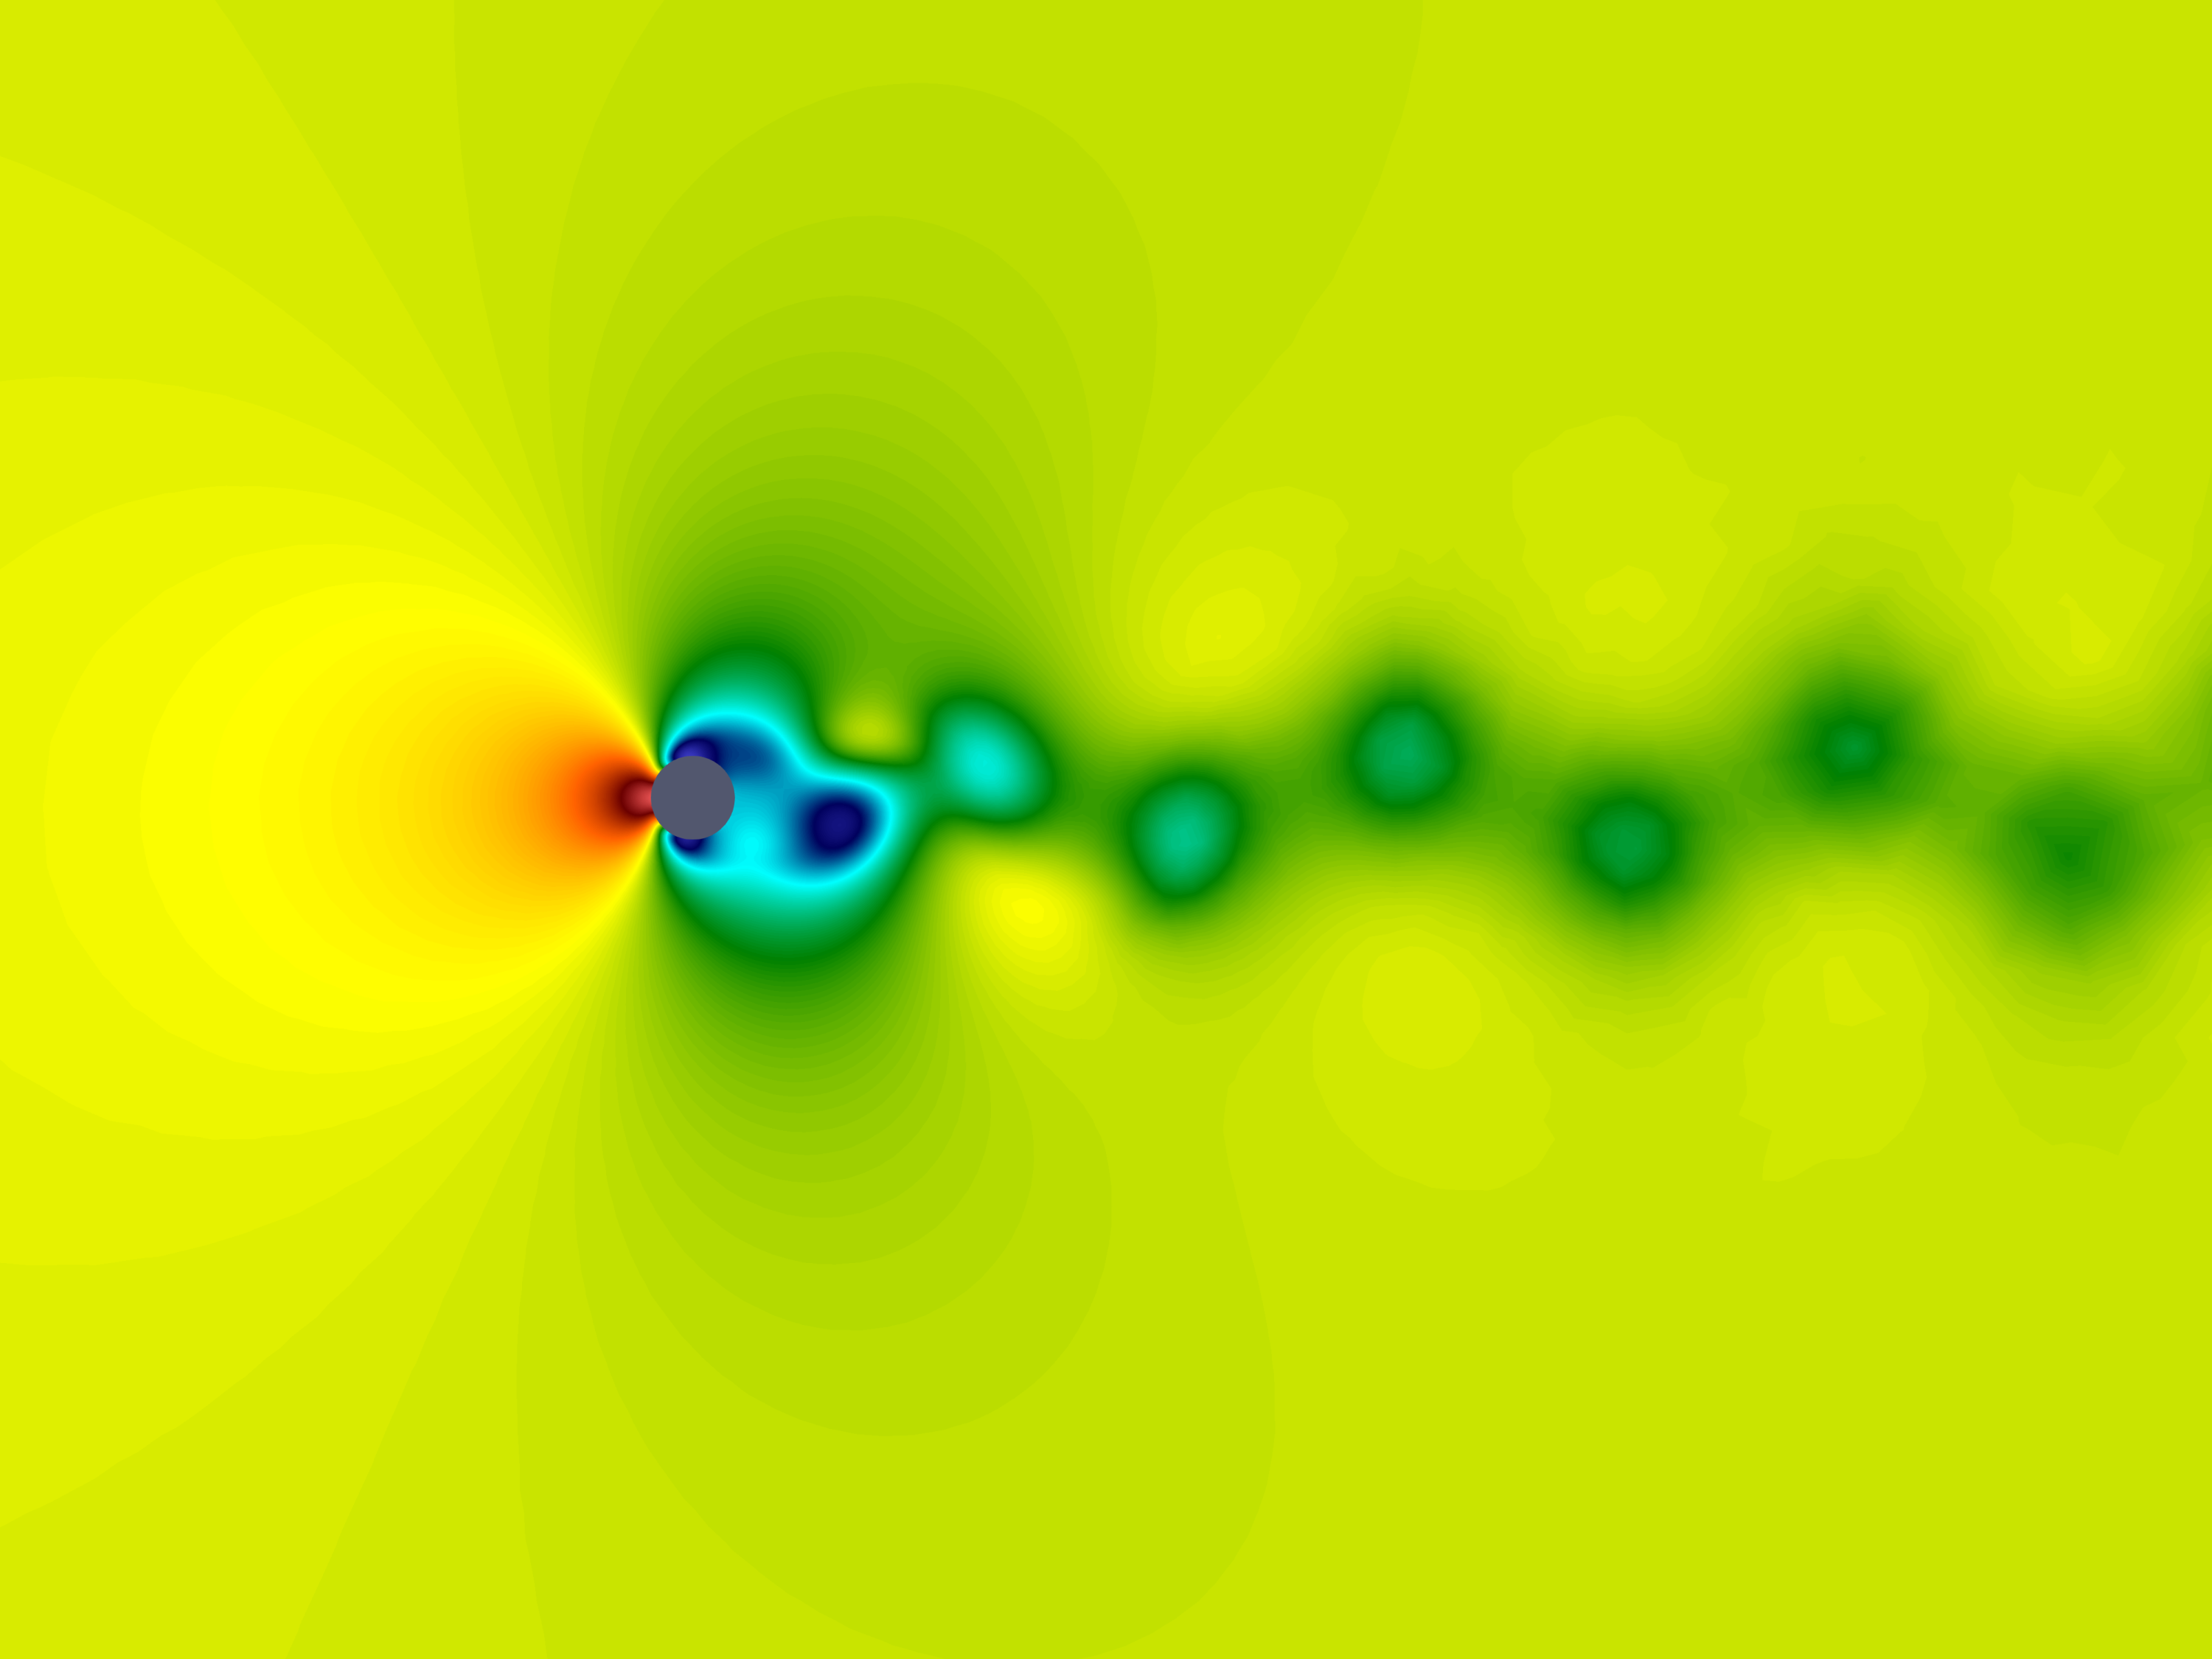
\includegraphics[scale=0.15,trim=5cm 5cm 5cm 6cm, clip=true]{Imagens/Cap2/cilindro_press2050.pdf}} \\
	\subfloat[$T_n + 2T_n/3$]{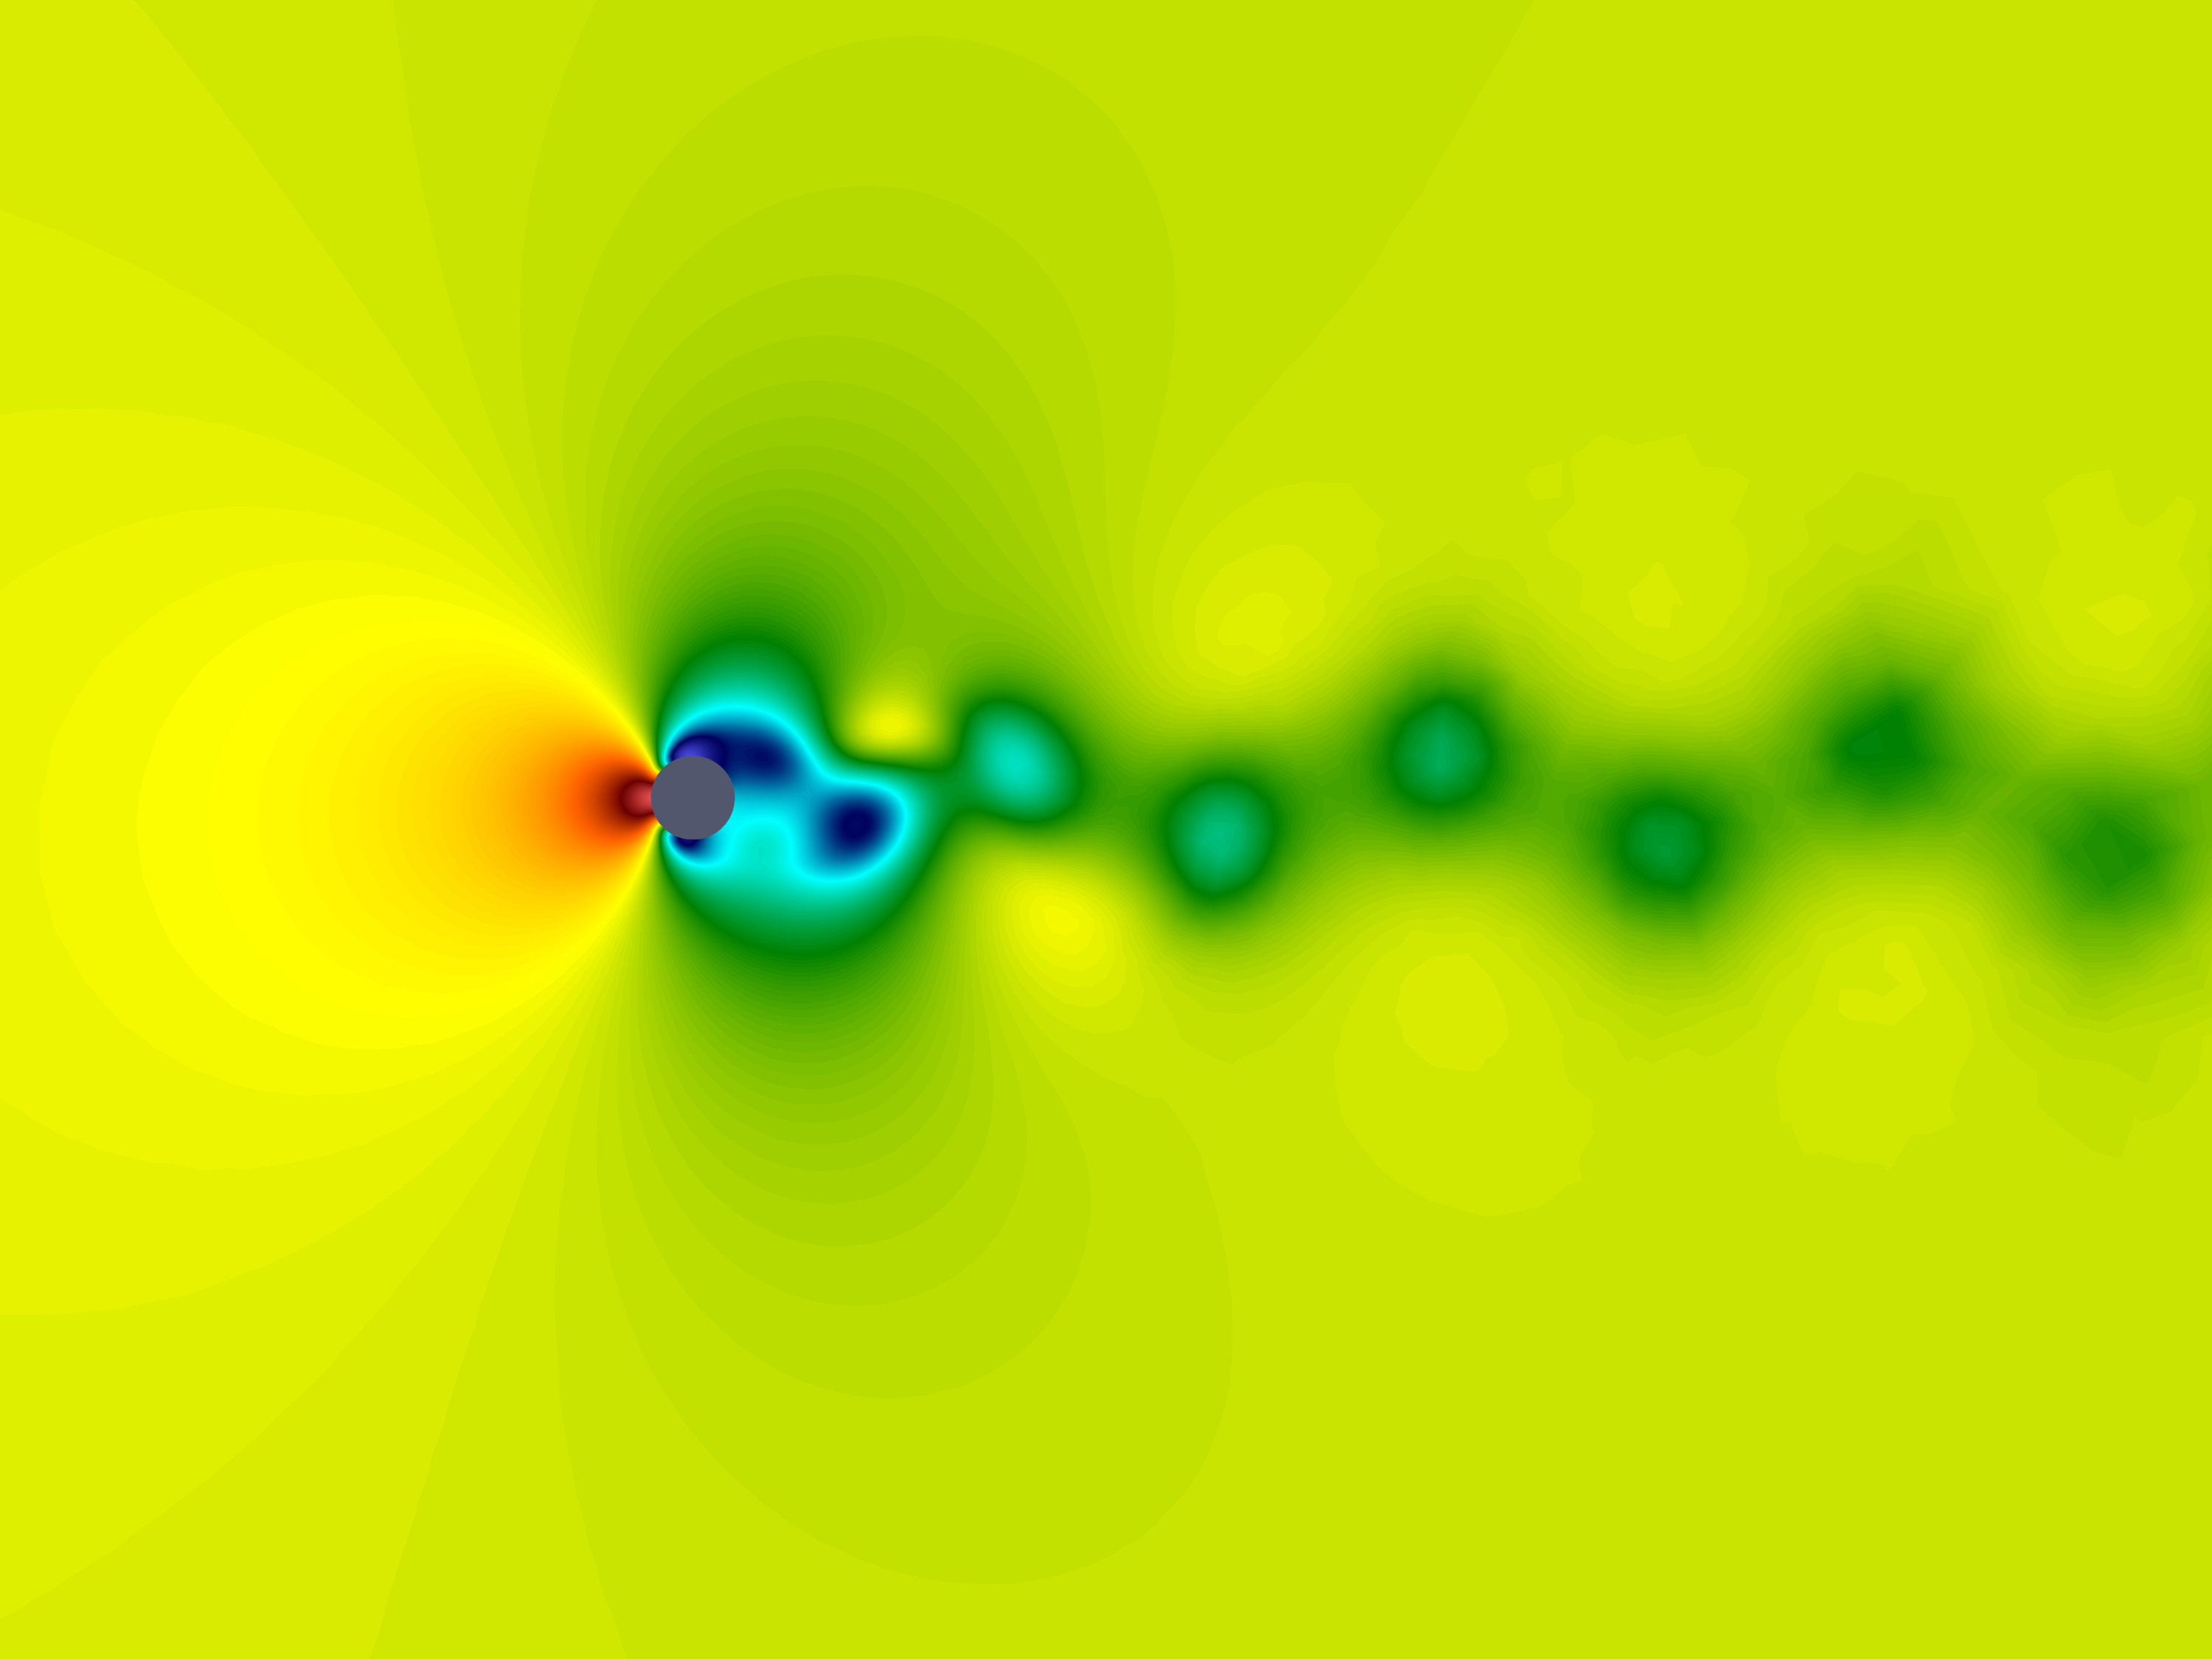
\includegraphics[scale=0.15,trim=5cm 5cm 5cm 6cm, clip=true]{Imagens/Cap2/cilindro_press2060.pdf}} \
	\subfloat[$T_n + 5T_n/6$]{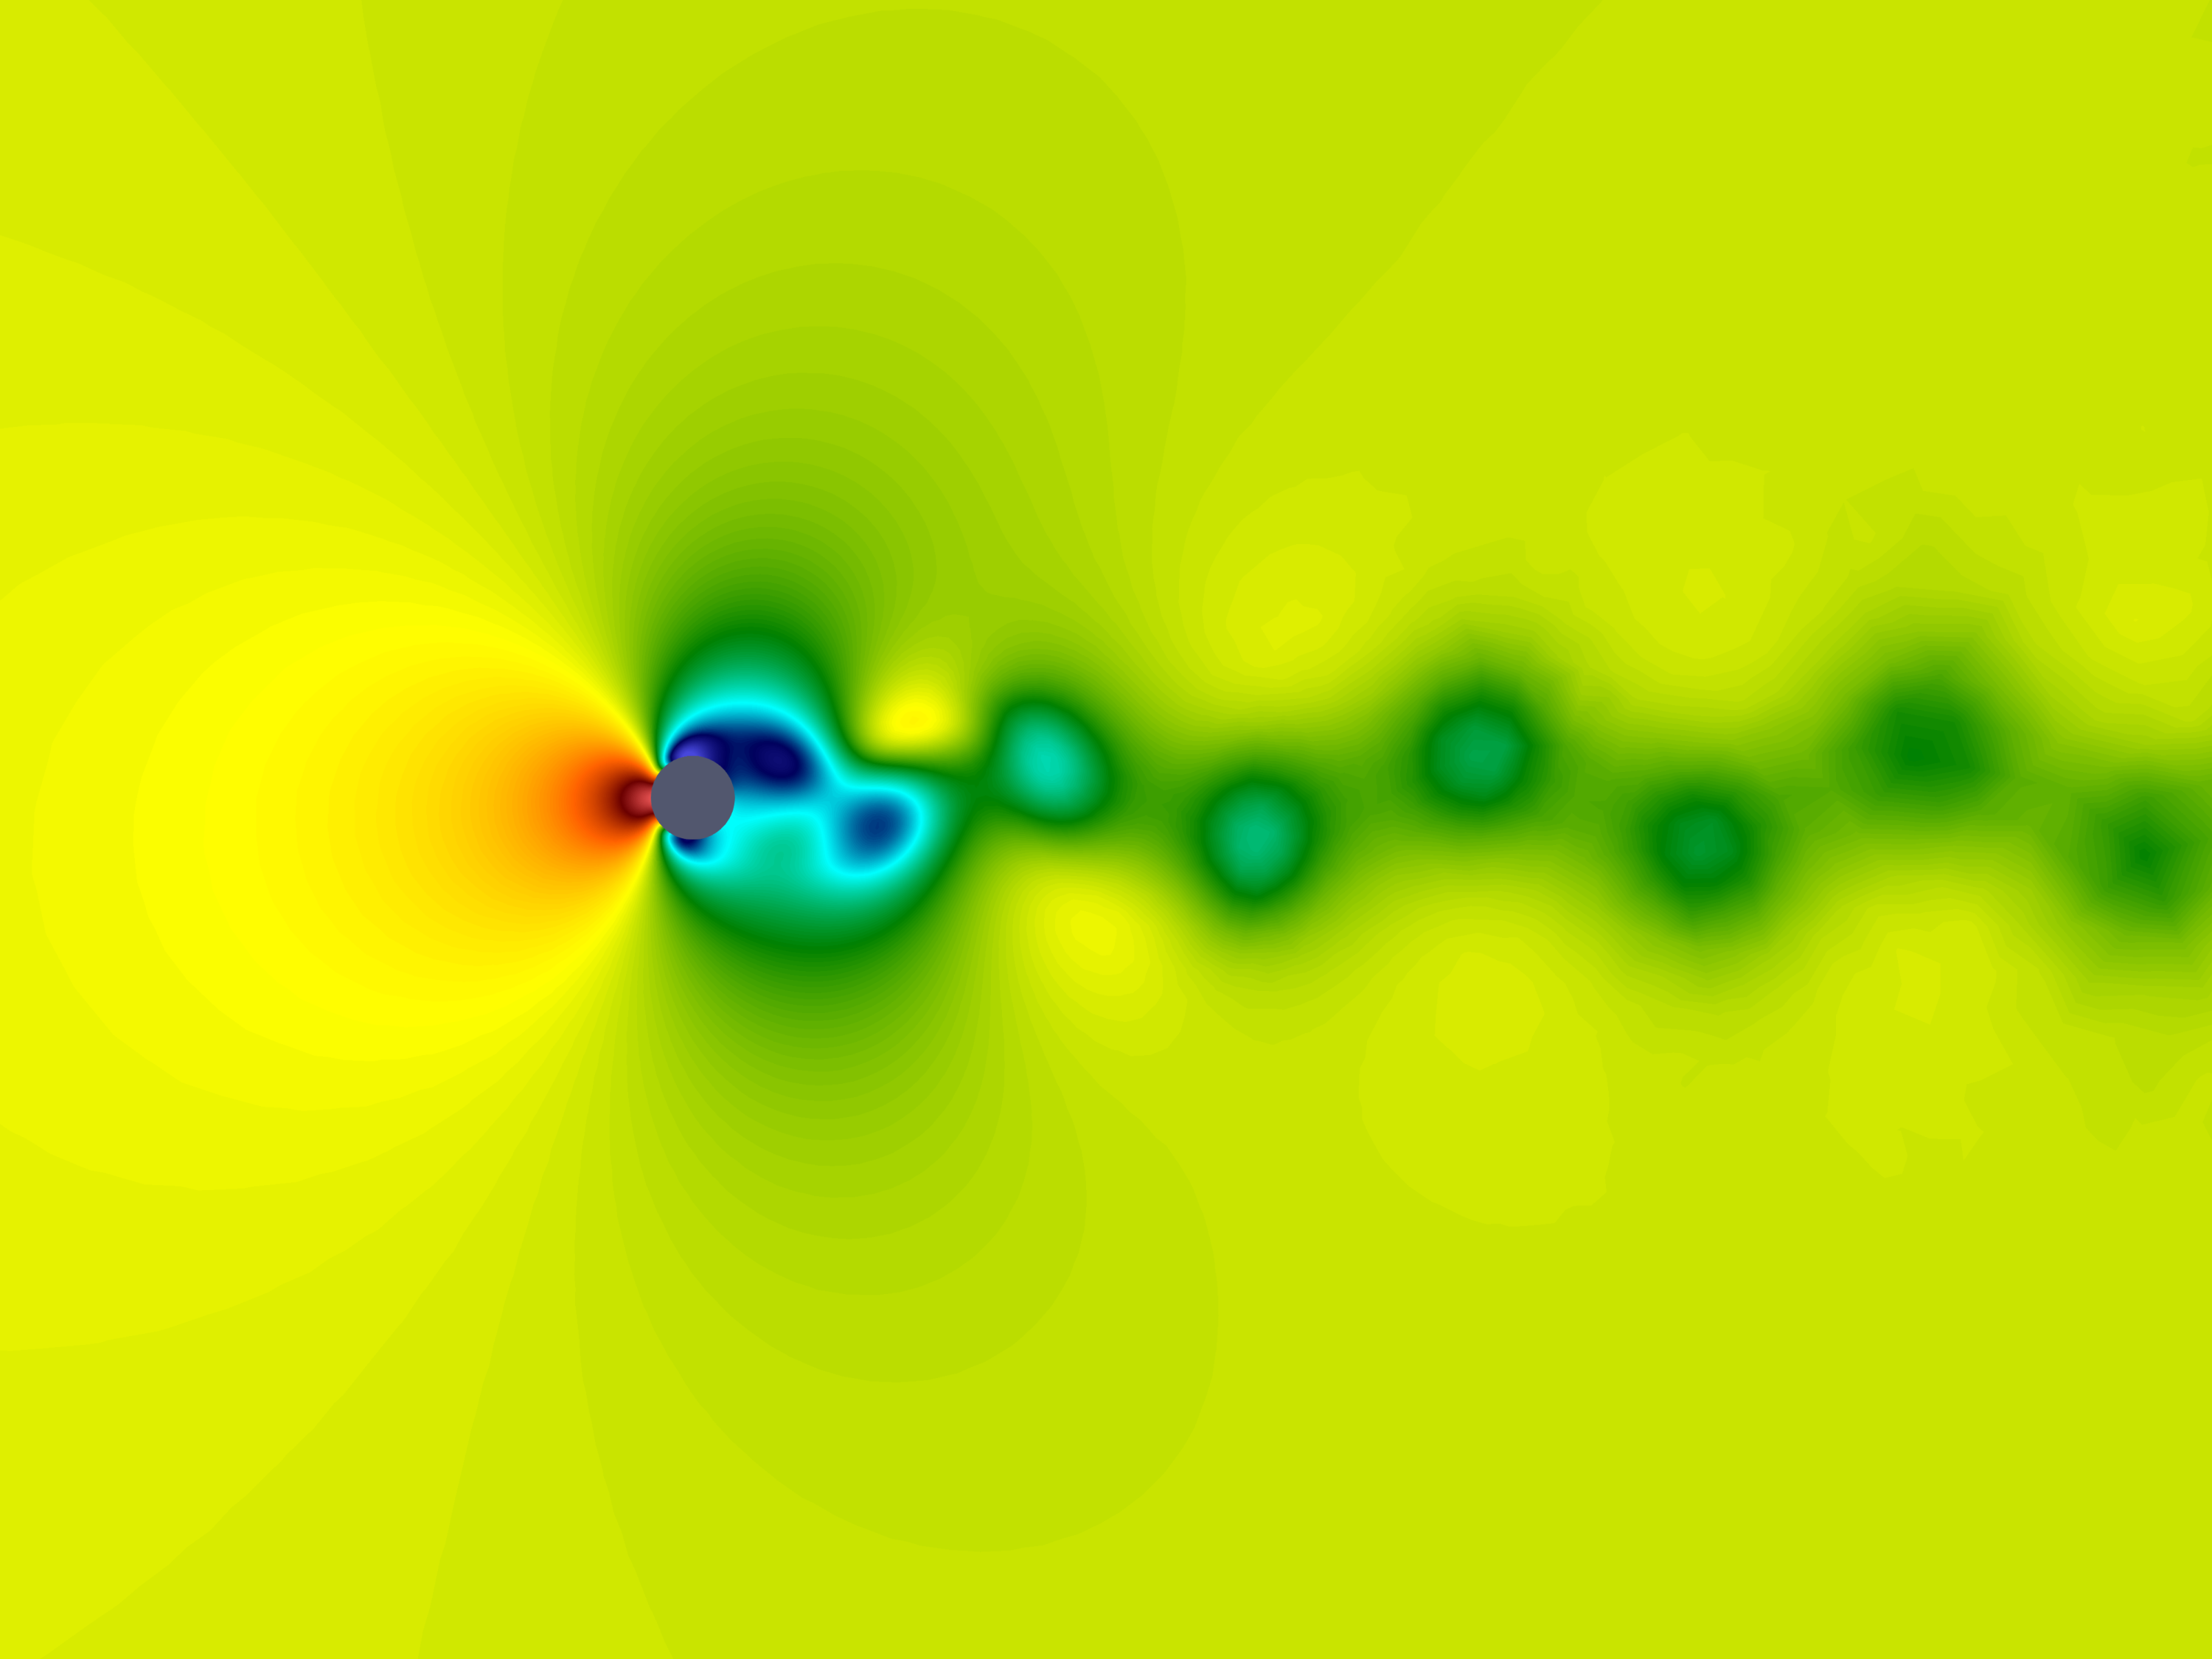
\includegraphics[scale=0.15,trim=5cm 5cm 5cm 6cm, clip=true]{Imagens/Cap2/cilindro_press2070.pdf}} \\
	{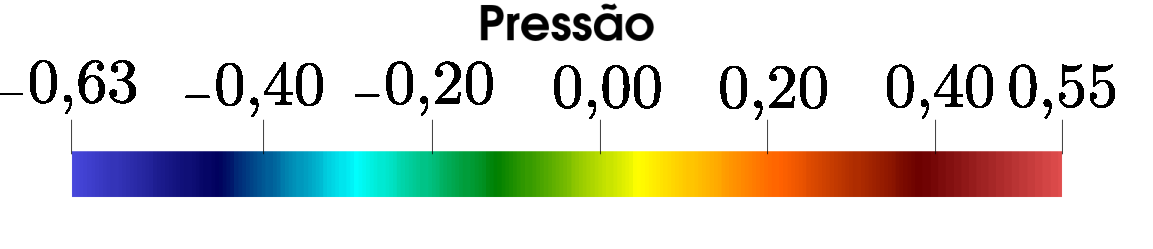
\includegraphics[trim=0cm 0cm 0cm 0cm,clip=true,scale=0.3]{Imagens/Cap2/cilindro_legendaPress.pdf}} \\
	\caption{Cilindro: Campos de pressão}
	\label{fig:cilindro_camposPressao}
\end{figure}


\subsection{Cavidade quadrada} \label{capitulo:Cap2:VerApl:CavQuad}

Para a verificação do código 3D utilizando elementos finitos o problema de uma cavidade quadrada com velocidade prescrita $u_{\infty}$ em sua parede superior foi estudado. A geometria do problema em questão e o conjunto de suas condições de contorno são apresentadas na Fig. \ref{fig:cavidade_geometria}. As paredes da cavidade são rígidas, com paredes laterais e do fundo com condição de aderência, e adicionalmente, condição de simetria na direção $y_3$. A cavidade possui na direção $y_3$ uma espessura de 0,03. A discretização espacial em elementos finitos utilizada é apresentada na Fig.  \ref{fig:cavidade_malha}, a qual consiste em 7252 elementos tetraédricos quadráticos e 14727 nós.

O problema é estudado para os números de Reynolds: 100, 400 e 1000. O número de Reynolds foi calculado de acordo com Eq. \eqref{eq:Reynolds}, com $L$ equivalente ao comprimento do lado da cavidade. O problema foi simulado para uma velocidade na parede superior de $u_{\infty} = 1,0$, $\density = 1,0$, $\timeStep = 0,05$, e $\specRadius = 0$, sendo a viscosidade do fluido variada de modo a alterar o número de Reynolds. A simulação foi mantida até que se atingiu o estado estacionário de escoamento. 

\begin{figure}[!htb]
	\centering
	\subfloat[Geometria e condições de contorno\label{fig:cavidade_geometria}]{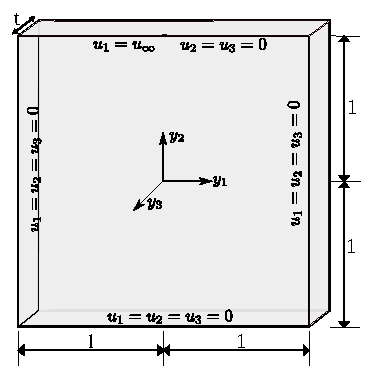
\includegraphics[scale=1.0,trim=0cm 0cm 0cm 0cm, clip=true]{Imagens/Cap2/cavidade_geometria.pdf}} \quad
	\subfloat[Discretização espacial.\label{fig:cavidade_malha}]{\includegraphics[trim=170 120 850 130,clip,scale=0.15]{Imagens/Cap2/cavidade_malha.png}}
	\caption{Cavidade quadrada: Geometria, condições de contorno e malha de elementos finitos}
\end{figure}

Os perfis de velocidade adimensionalizados ($\velocity/\velocinfty$) ao longo de duas linhas centrais nas direções $y_1$ e $y_2$ posicionadas no centro da espessura da direção $y_3$ da cavidade são apresentados na Fig. \ref{fig:cavidade_graficos} e comparados com a referência de \citeonline{GhiaGS:1982}.


\begin{figure}[!t]
	\centering
	\subfloat[\label{fig:cavidade_Re100}$Re$=100]{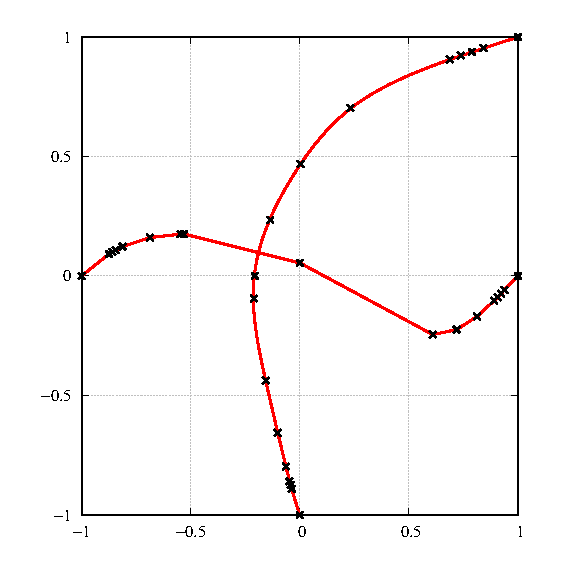
\includegraphics[scale=.8,trim=0.55cm 0cm 0.3cm 0.2cm, clip=true]{Imagens/Cap2/cavidade_Re100.eps}} \subfloat[\label{fig:cavidade_Re400}$Re$=400]{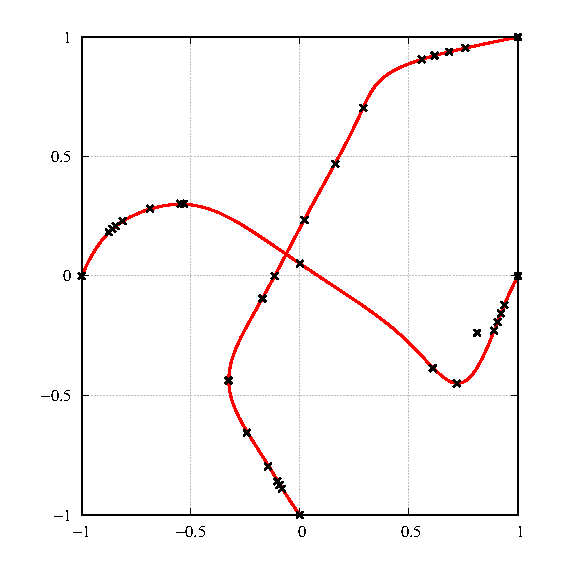
\includegraphics[scale=.8,trim=0.55cm 0cm 0.3cm 0.2cm, clip=true]{Imagens/Cap2/cavidade_Re400.eps}}\\ 
	\subfloat[\label{fig:cavidade_Re1000}$Re$=1000]{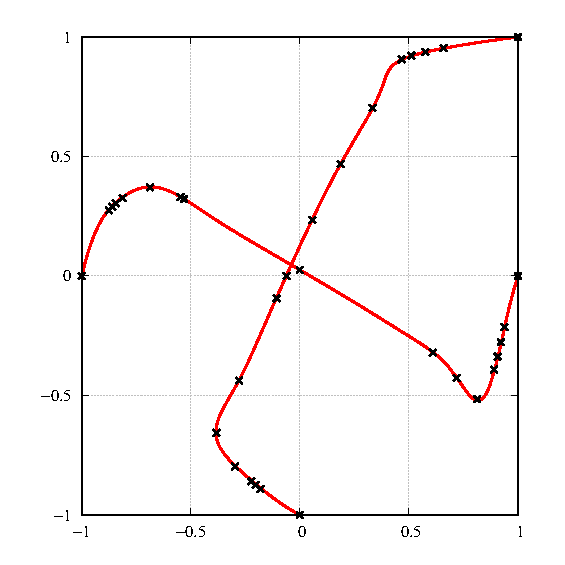
\includegraphics[scale=.8,trim=0.55cm 0cm 0.3cm 0.2cm, clip=true]{Imagens/Cap2/cavidade_Re1000.eps}} \\
	\subfloat{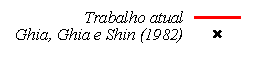
\includegraphics[scale=1.]{Imagens/Cap2/cavidade_legenda.pdf}} 
	\caption{Cavidade quadrada: Perfis de velocidade adimensionalizados nas direções $y_1$ e $y_2$  }
	\label{fig:cavidade_graficos}
\end{figure}

Os campos de velocidade e de pressão são apresentados nas figuras Fig \ref{fig:cavidade_vel} e \ref{fig:cavidade_press} respectivamente. Ressalta-se que para a solução do problema, por se tratar de um problema com todos os contornos com condição de Dirichlet impostos, a pressão torna-se indefinida. Por esse motivo, prescreveu-se uma pressão $\press = \press_{ref} =  0.0$ no canto superior direito da cavidade. 


\begin{figure}[!t]
	\centering
	\setlength{\lineskip}{-10pt}
	\subfloat[\label{fig:cavidade_vel_Re100}$Re$=100]{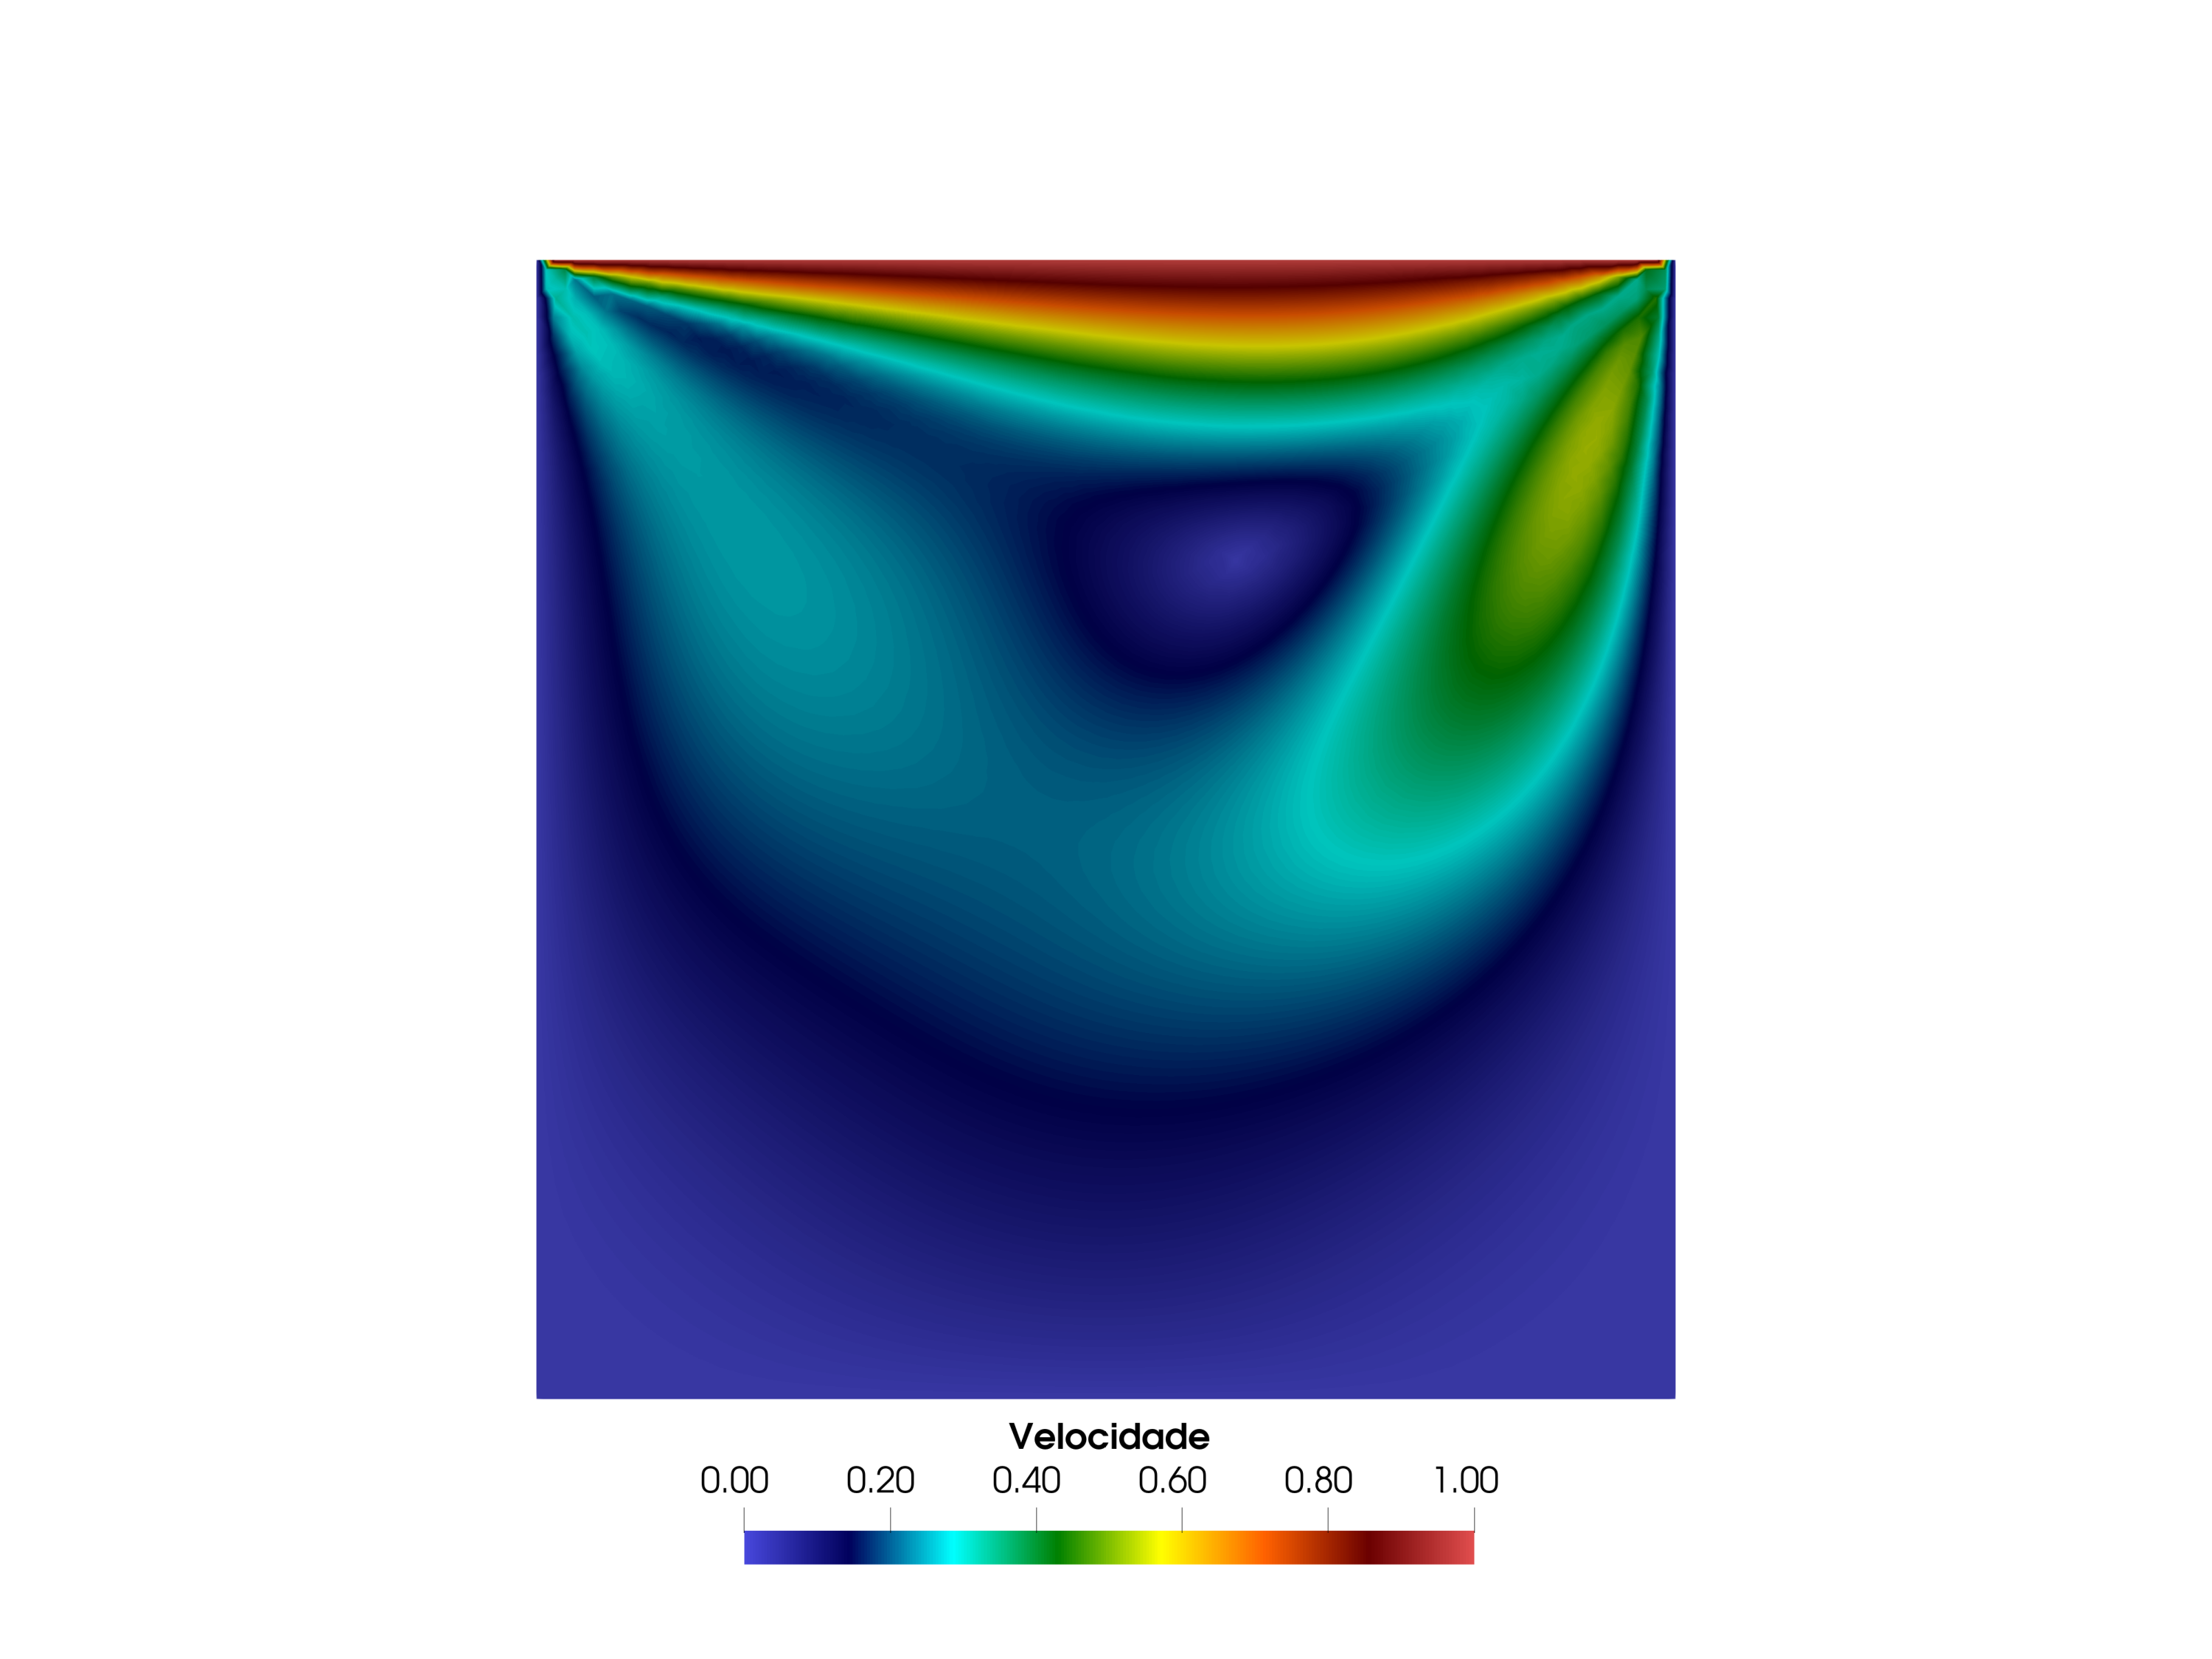
\includegraphics[scale=0.25,trim=12cm 5.5cm 12cm 5cm, clip=true]{Imagens/Cap2/cavidade_velRe100.pdf}} 
	\subfloat[\label{fig:cavidade_vel_Re400}$Re$=400]{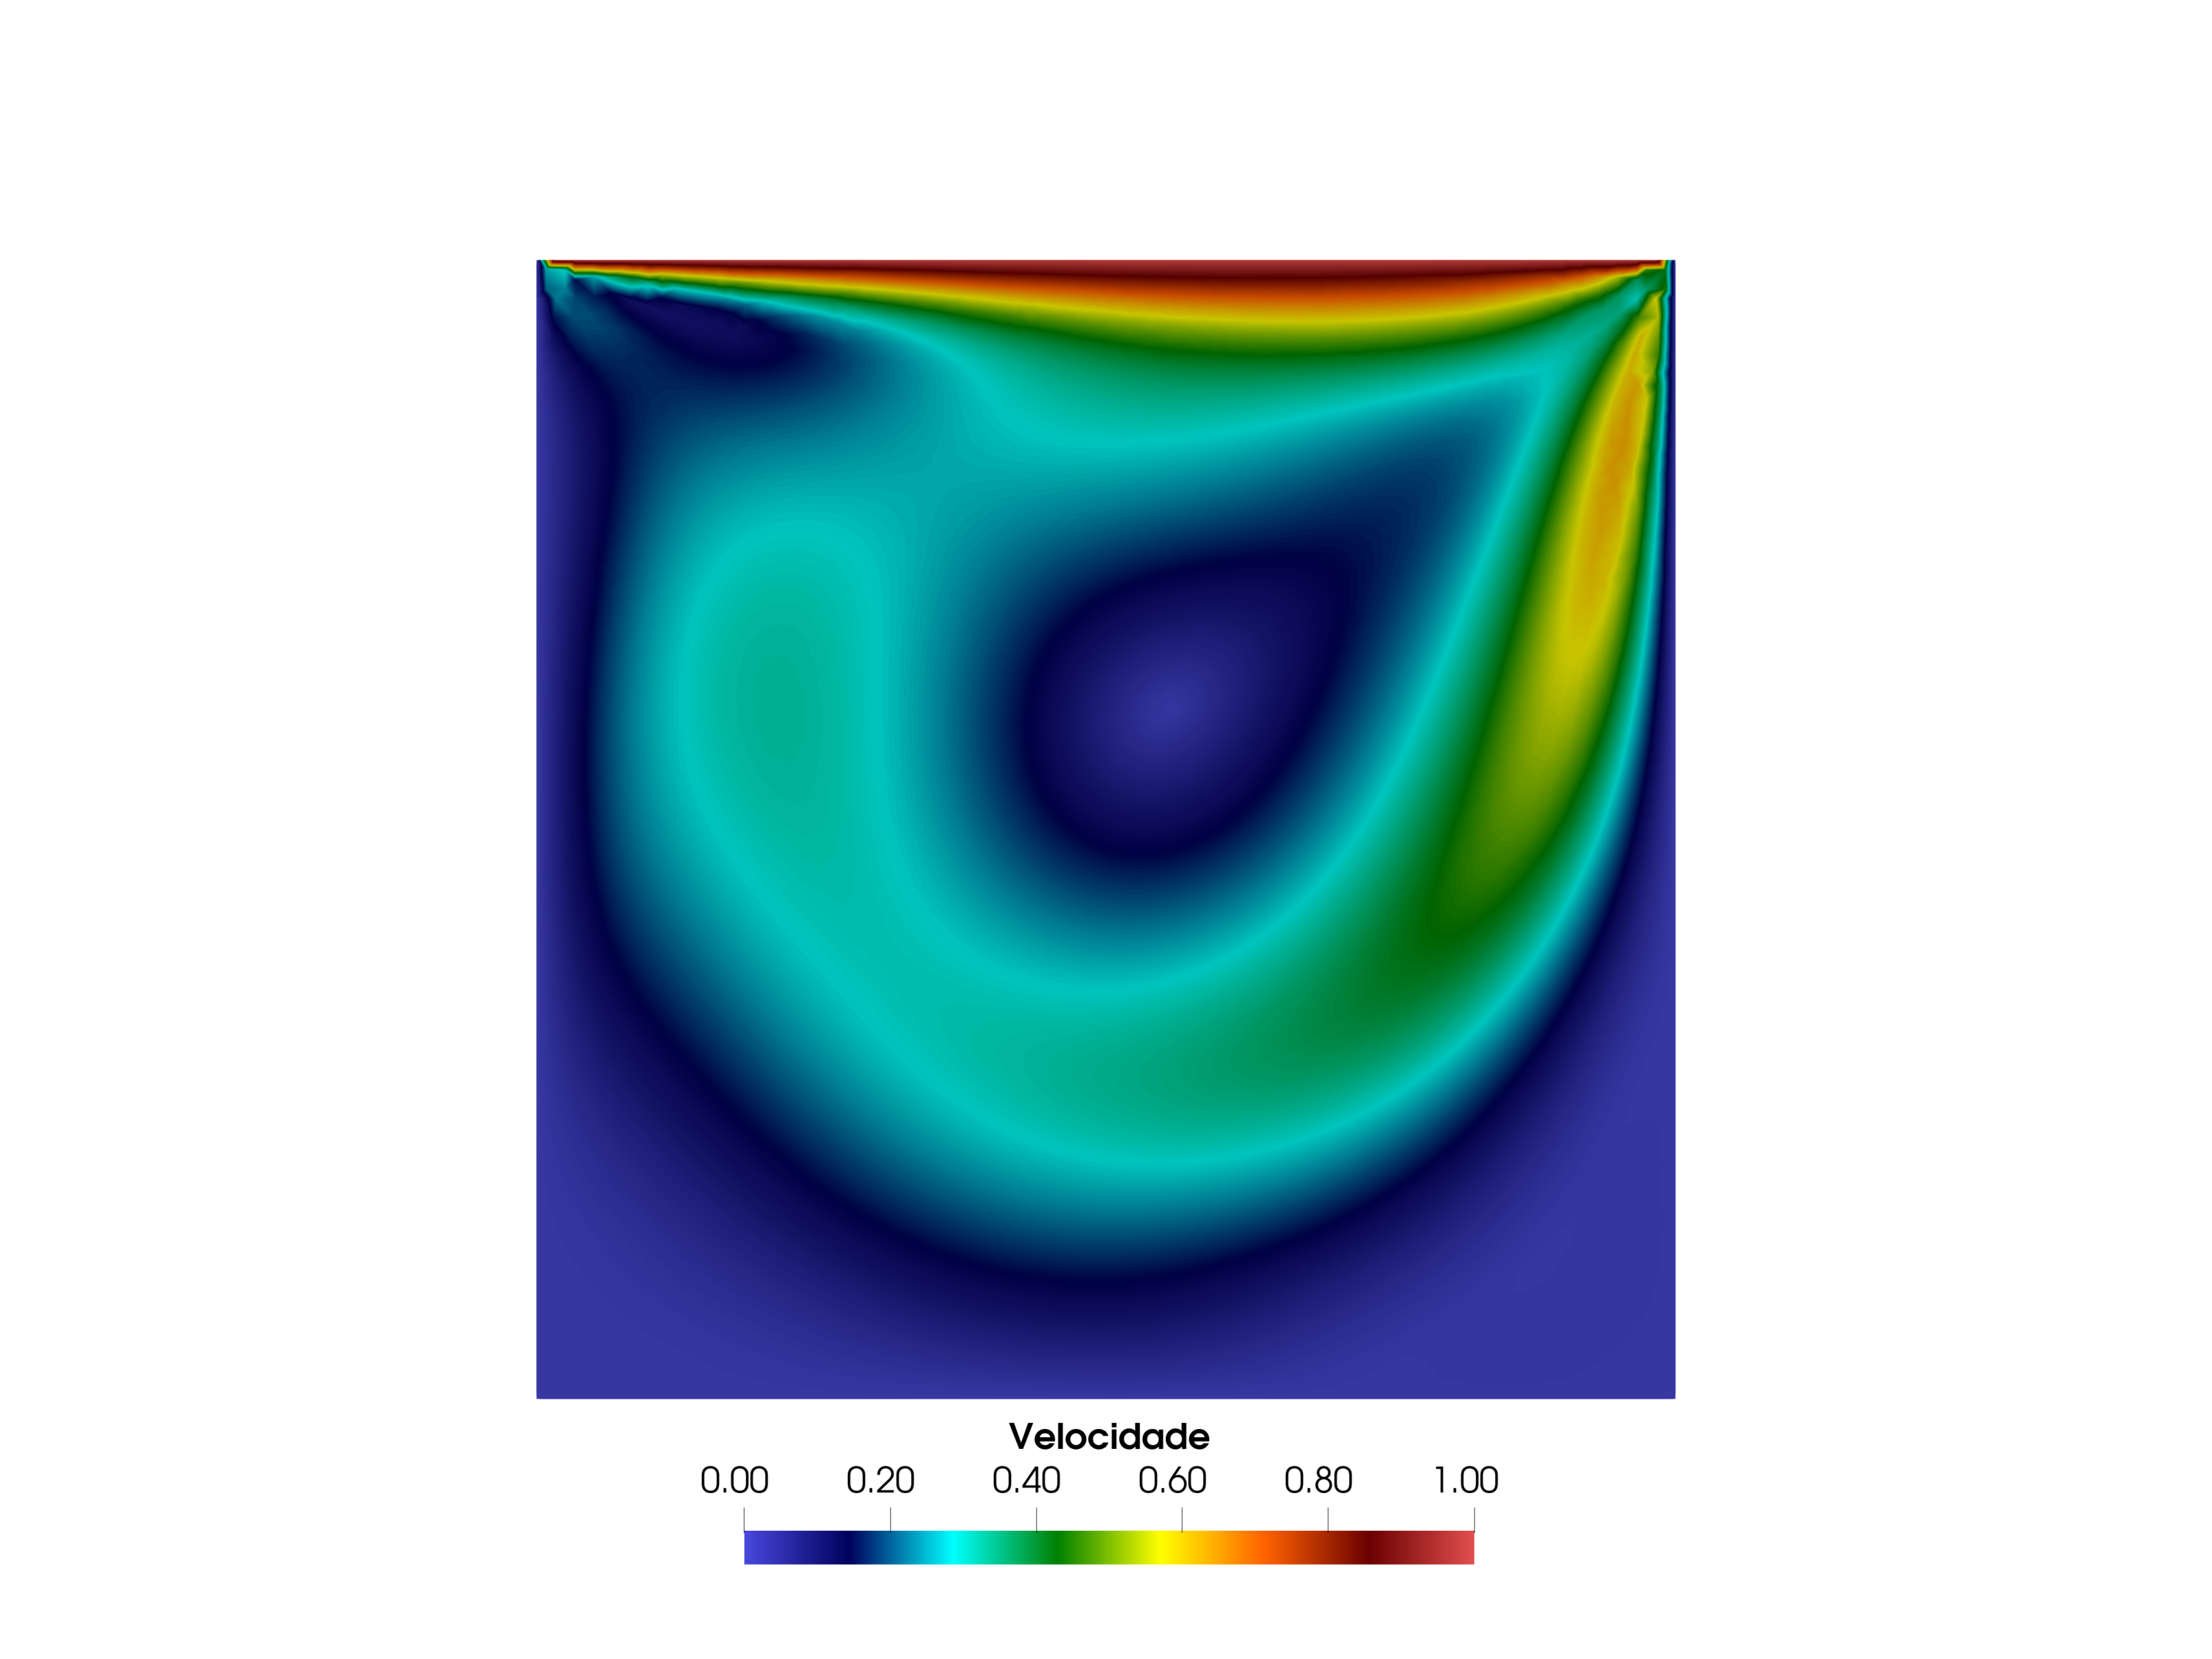
\includegraphics[scale=0.25,trim=12cm 5.5cm 12cm 5cm, clip=true]{Imagens/Cap2/cavidade_velRe400.pdf}}\\ 
	\subfloat[\label{fig:cavidade_vel_Re1000}$Re$=1000]{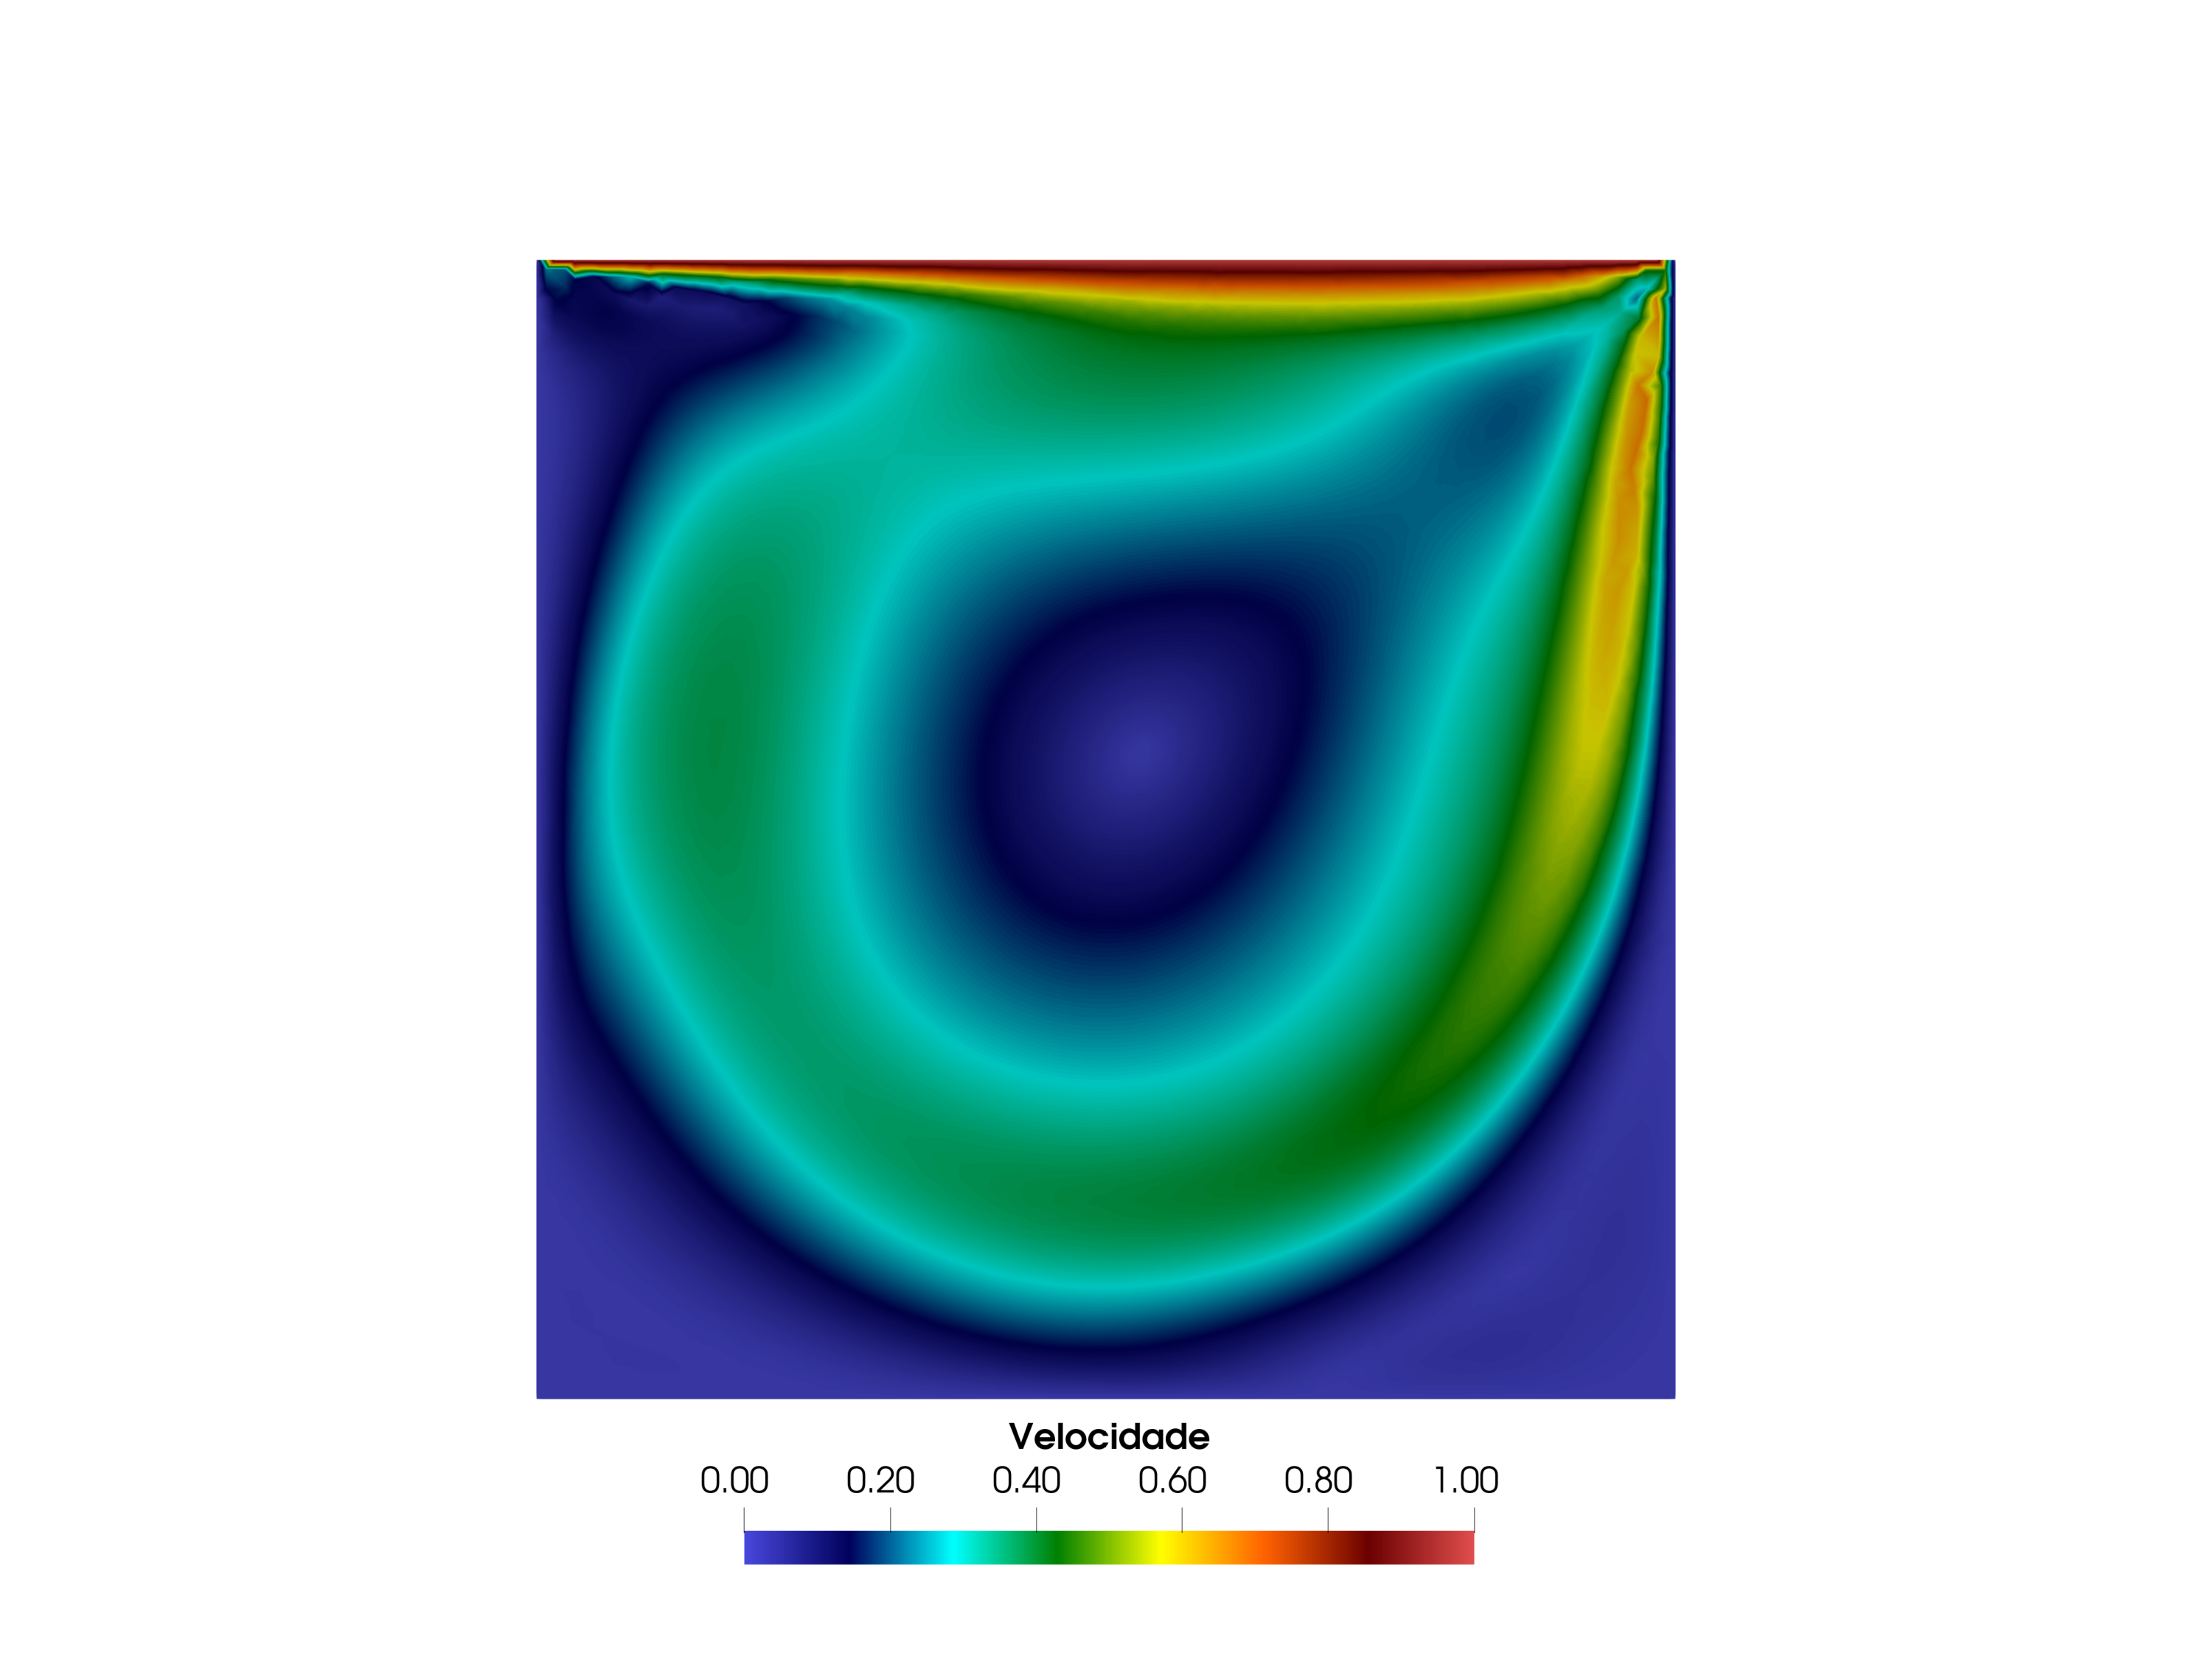
\includegraphics[scale=0.25,trim=12cm 5.5cm 12cm 5cm, clip=true]{Imagens/Cap2/cavidade_velRe1000.pdf}}\\[3.0ex]
	% Barra de cores (legenda) separada
	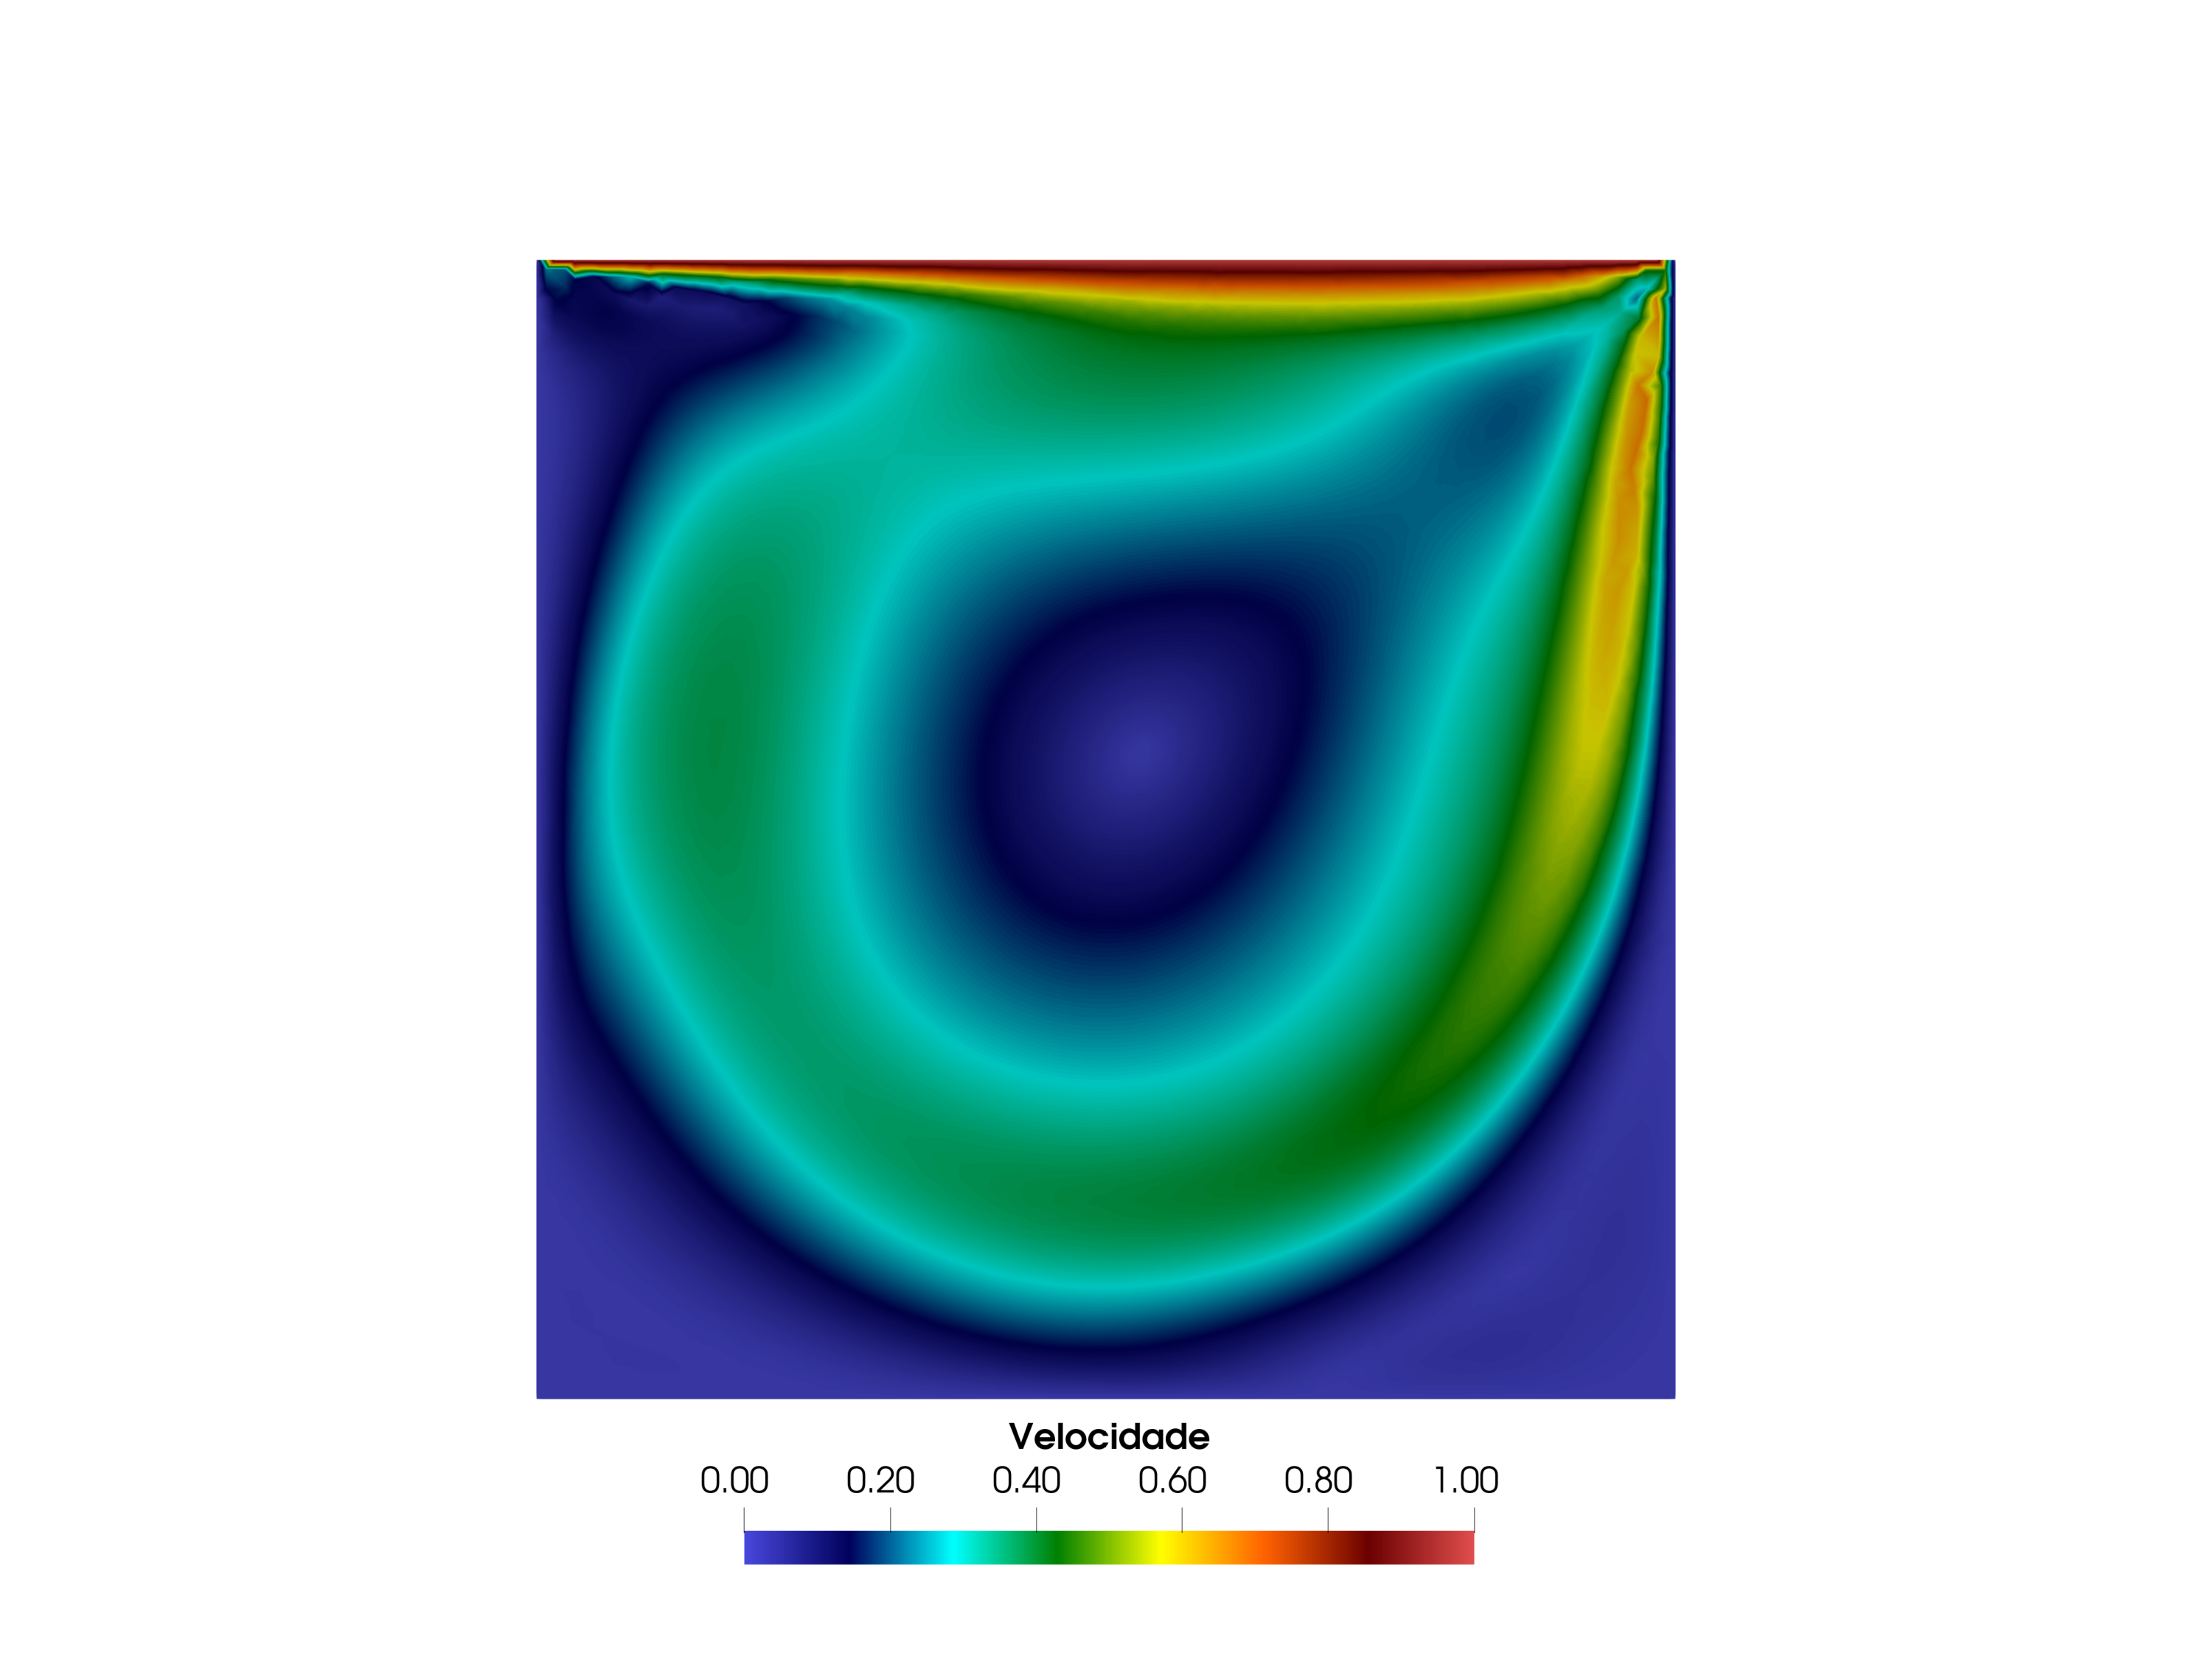
\includegraphics[scale=0.4,trim=12cm 0cm 12cm 32.5cm, clip=true]{Imagens/Cap2/cavidade_velRe1000.pdf}
	
	\caption{Cavidade quadrada: Campos de velocidade.}
	\label{fig:cavidade_vel}
\end{figure}

\begin{figure}[!t]
	\centering
	\setlength{\lineskip}{-10pt}
	\subfloat[\label{fig:cavidade_press_Re100}$Re$=100]{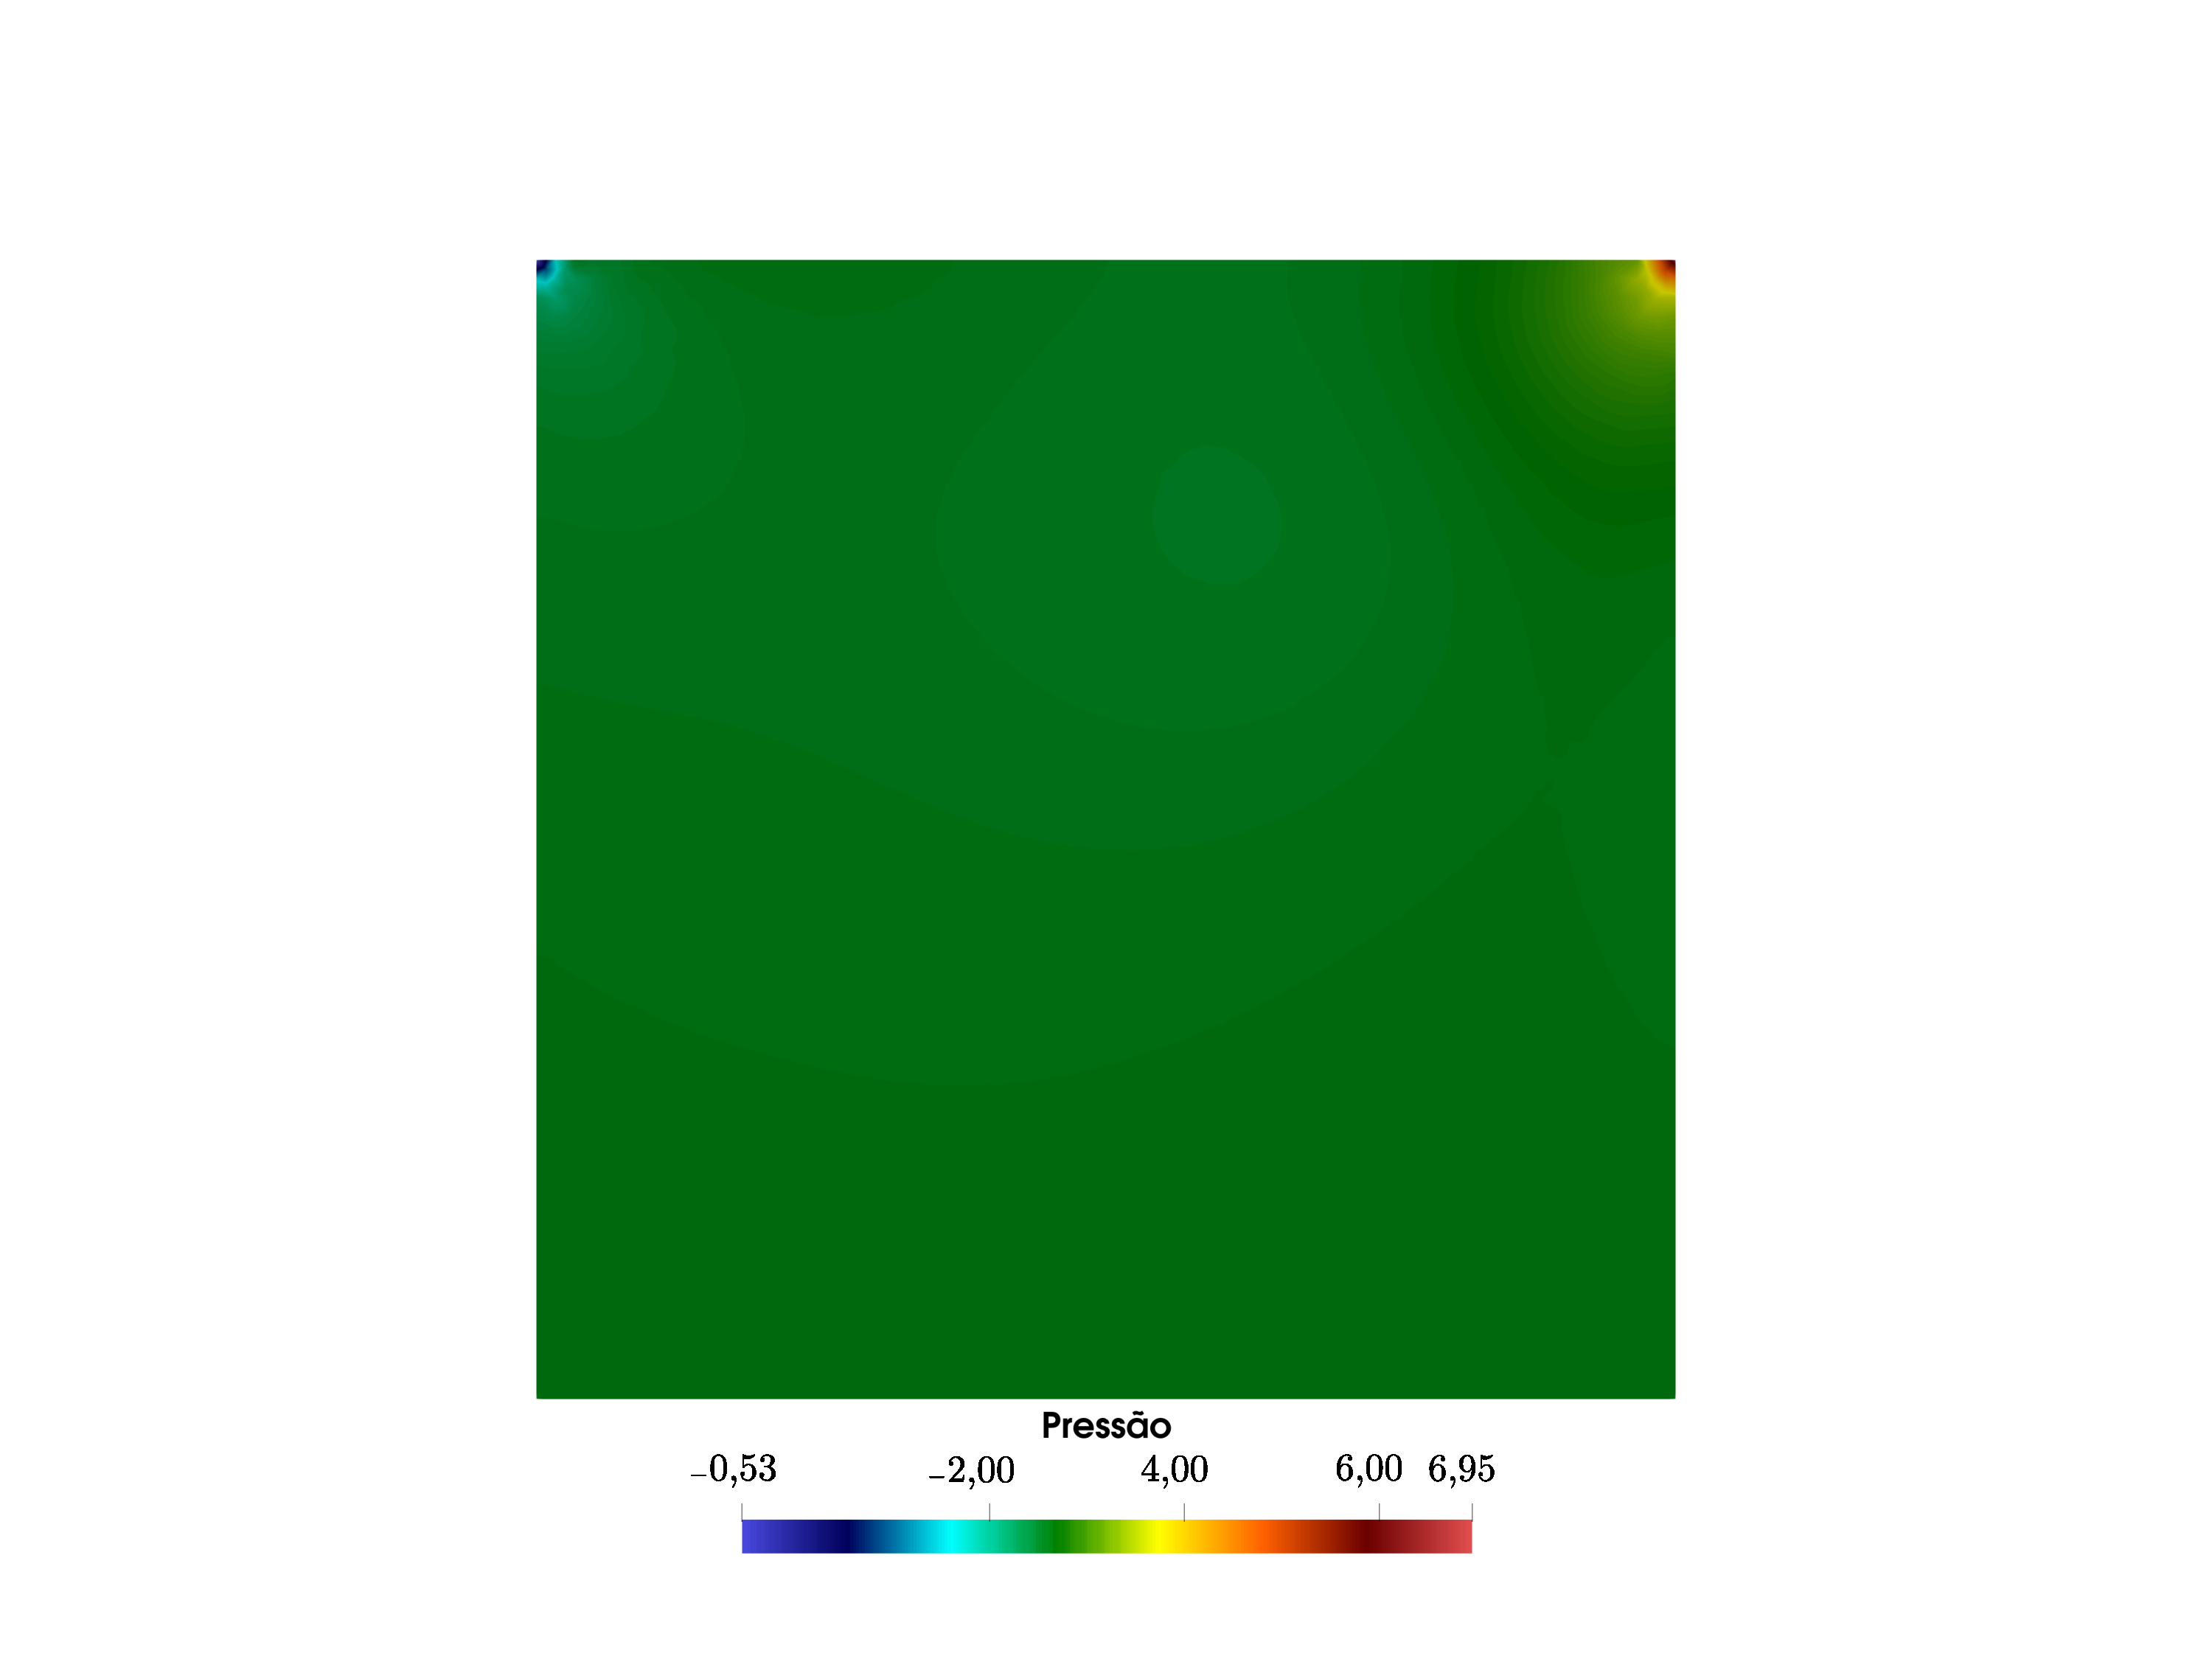
\includegraphics[scale=0.25,trim=12cm 2cm 12cm 5cm, clip=true]{Imagens/Cap2/cavidade_pressRe100.pdf}} 
	\subfloat[\label{fig:cavidade_press_Re400}$Re$=400]{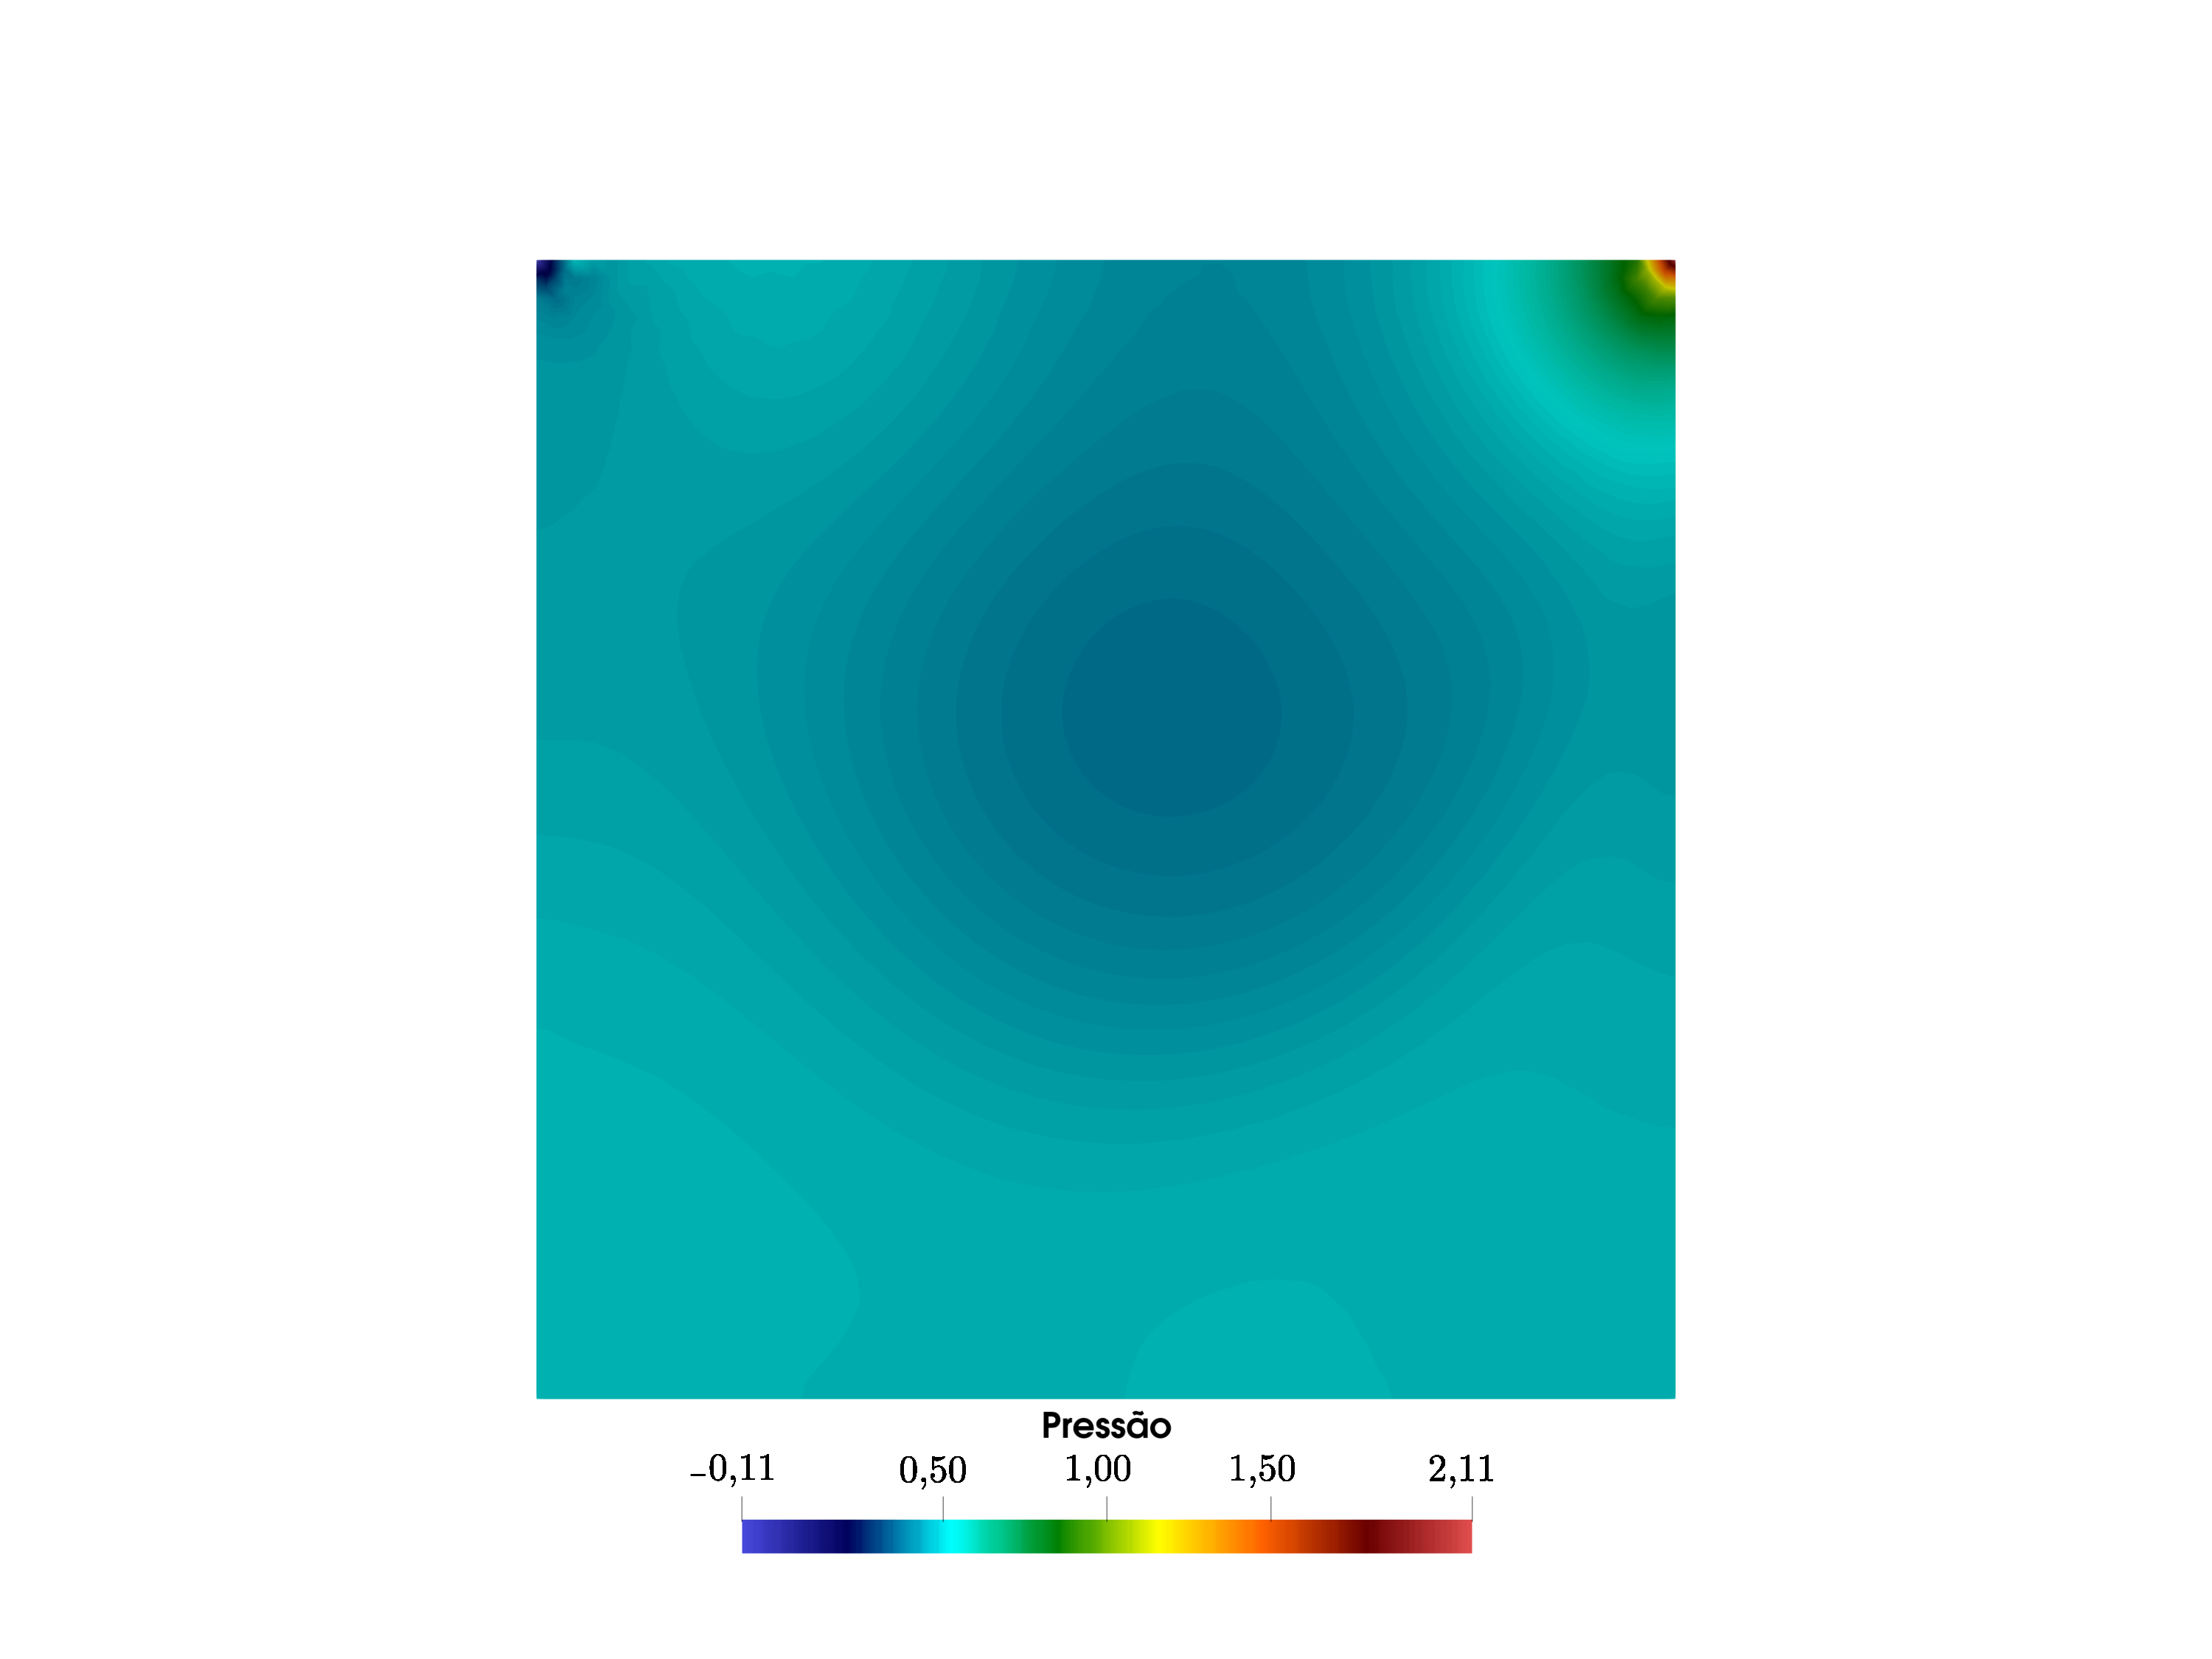
\includegraphics[scale=0.25,trim=12cm 2cm 12cm 5cm, clip=true]{Imagens/Cap2/cavidade_pressRe400.pdf}}\\ 
	\subfloat[\label{fig:cavidade_press_Re1000}$Re$=1000]{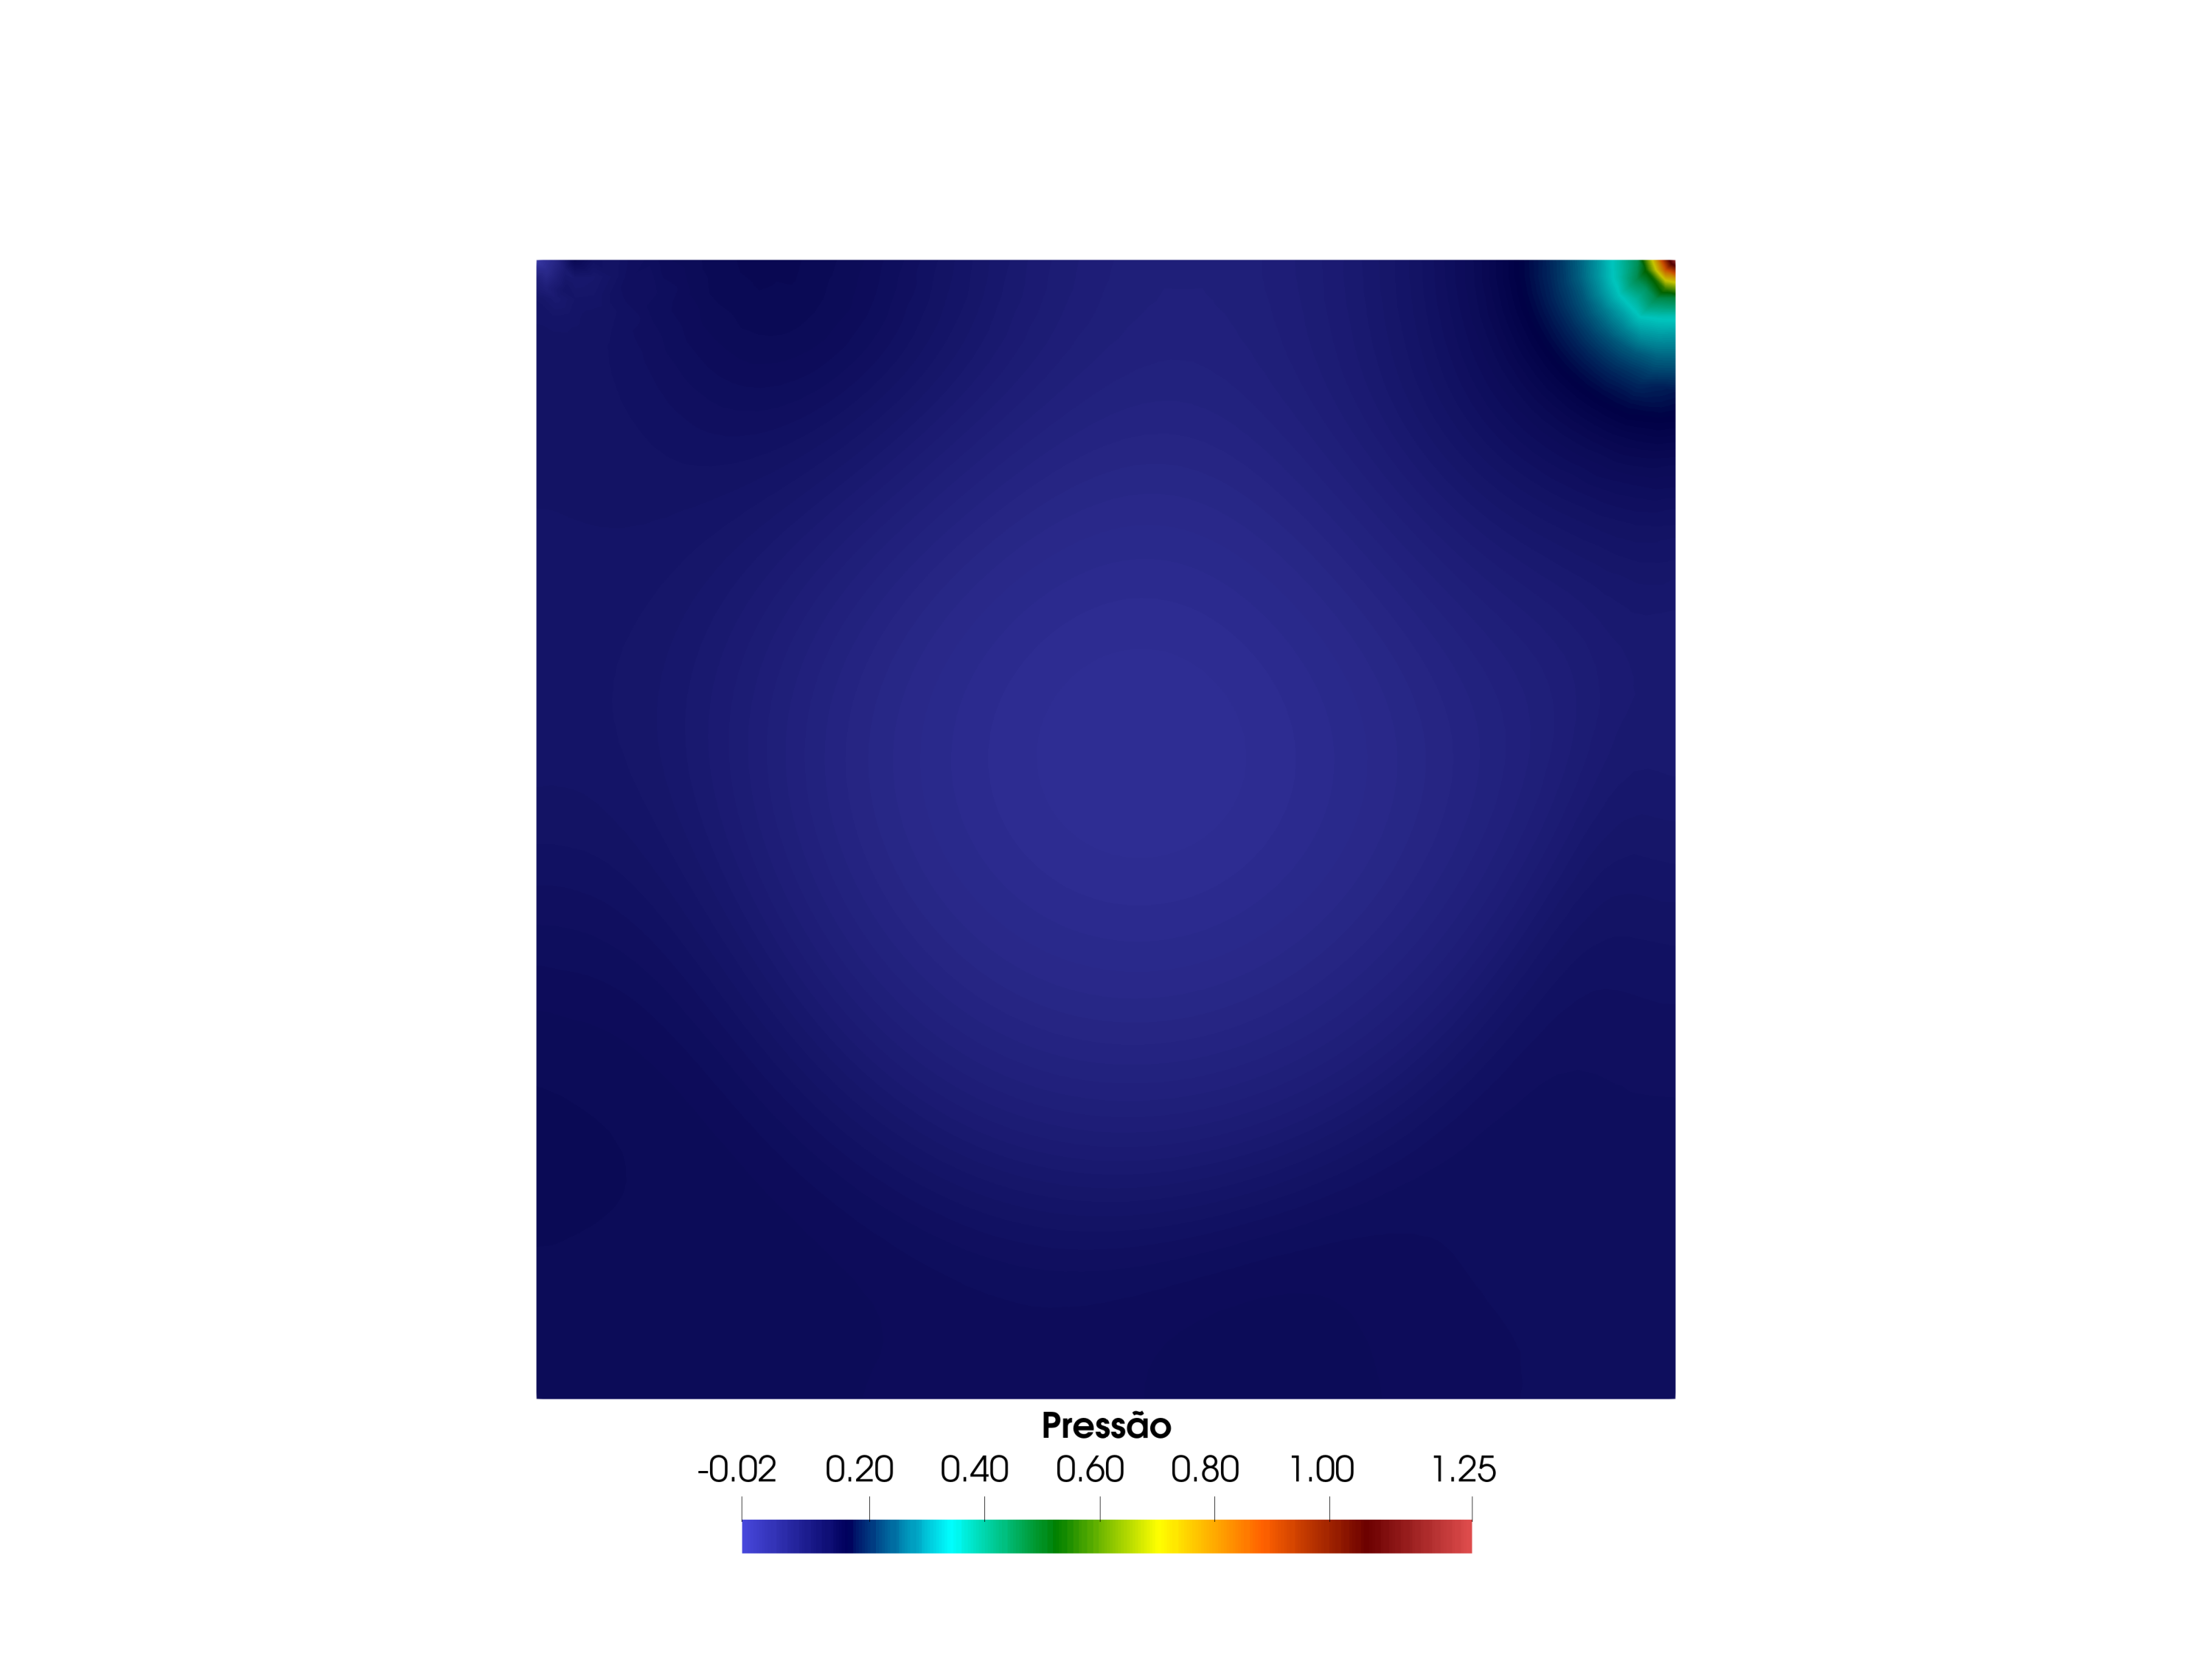
\includegraphics[scale=0.25,trim=12cm 2cm 12cm 5cm, clip=true]{Imagens/Cap2/cavidade_pressRe1000.pdf}}
	\caption{Cavidade quadrada: Campos de pressão.}
	\label{fig:cavidade_press}
\end{figure}



%
%\clearpage[e ]
%
%\textcolor{white}{ }


\end{document}

% !TeX spellcheck = pt_BR
\documentclass[tese_patricia]{subfiles}
\begin{document}

% ---------------------------------------------------------- 
% Métodos de malhas sobrepostas
% ----------------------------------------------------------
\chapter[Análise isogeométrica aplicada à Mecânica dos Fluidos]{Análise isogeométrica aplicada à Mecânica dos Fluidos} \label{capitulo:Cap3}
% ----------------------------------------------------------

%\nomenclature[C,01]{$p$}{Grau das funções base na direção paramétrica $\xsi$;}
%\nomenclature[C,02]{$\xsi$}{Vetor de \textit{knots} na direção paramétrica $\xsi$;}
%\nomenclature[C,03]{$\xsi$}{Uma das direções paramémtricas nas quais as funções base são definidas;}
%\nomenclature[C,04]{$n$}{Número de funções base na direção paramétrica $\xsi$ ;}
%\nomenclature[C,05]{$N$}{Função base \textit {B-Spline} na direção paramétrica $\xsi$ ;}
%\nomenclature[C,06]{$\CP$}{Pontos de controle que descrevem a geometria \textit{B-Spline} ou NURBS;}
%\nomenclature[C,07]{$\mathbf{C}$}{Curva \textit {B-Spline} ou NURBS;}
%\nomenclature[C,08]{$m$}{Grau das funções base na direção paramétrica $\eta$;}
%\nomenclature[C,09]{$\mathcal{H}$}{Vetor de \textit{knots} na direção paramétrica $\eta$;}
%\nomenclature[C,10]{$q$}{Número de funções base na direção paramétrica $\eta$ ;}
%\nomenclature[C,11]{$\eta$}{Uma das direções paramémtricas nas quais as funções base são definidas;}
%\nomenclature[C,12]{$M$}{Função base \textit {B-Spline} na direção paramétrica $\eta$ ;}
%\nomenclature[C,13]{$\mathbf{S}$}{Superfície \textit {B-Spline} ou NURBS;}
%\nomenclature[C,14]{$\hat{N}$}{Função \textit {B-Spline} fruto do produto tensorial entre funções base descritas em um espaço paramétrico qualquer;}
%\nomenclature[C,15]{$L$}{Função base \textit {B-Spline} na direção paramétrica $\zeta$ ;}
%\nomenclature[C,16]{$r$}{Grau das funções base na direção paramétrica $\zeta$;}
%\nomenclature[C,17]{$\mathcal{Z}$}{Vetor de \textit{knots} na direção paramétrica $\zeta$;}
%\nomenclature[C,18]{$\zeta$}{Uma das direções paramémtricas nas quais as funções base são definidas;}
%\nomenclature[C,19]{$l$}{Número de funções base na direção paramétrica $\zeta$ ;}
%\nomenclature[C,20]{$\mathbf{T}$}{Sólido \textit {B-Spline} ou NURBS;}
%\nomenclature[C,21]{$\mathbf{C}^{w}$}{Curva \textit{B-Spline} no $\realspace^{d+1}$ cuja projeção transformativa gera uma curva \mathbf{C} no $\realspace^{d}$;}
%\nomenclature[C,22]{$R$}{Função base NURBS;}
%\nomenclature[C,23]{$w$}{Peso respectivo a um ponto de controle;}
%\nomenclature[C,24]{$\mathbf{\hat{\xsi}}$}{Coordenadas do espaço parental, no qual realiza-se a integração numérica;}
%\nomenclature[C,25]{$\hat{\xsi}$}{Uma das direções do espaço parental;}
%\nomenclature[C,26]{$\hat{\eta}$}{Uma das direções do espaço parental;}
%\nomenclature[C,27]{$\hat{\zeta}$}{Uma das direções do espaço parental;}
%\nomenclature[C,28]{$\tilde{\Omega^{e}}$}{Domínio de uma célula no espaço paramétrico;}
%\nomenclature[C,29]{$\hat{\Omega^{e}}$}{Domínio de um uma célula o no espaço parental;}
%\nomenclature[C,30]{$h$}{Dimensão na direção $y$ da entrada do perfil parabólico no problema do escoamento sobre canal com degrau;}
%\nomenclature[C,31]{$s$}{Dimensão  na direção $y$ do degrau que compõe o problema do escoamento sobre canal com degrau;}
%\nomenclature[C,32]{$x_{e}$}{Dimensão na direção $x$  do degrau que compõe o problema do escoamento sobre canal com degrau;}
%\nomenclature[C,33]{$x_{f}$}{Dimensão na direção $x$  do \textit{patch} $P1$ do problema do escoamento sobre canal com degrau;}
%\nomenclature[C,34]{$x_{t}$}{Dimensão do canal após o degrau na direção $x$ do problema do escoamento sobre canal com degrau;}
%\nomenclature[C,35]{$V_{max}$}{Velocidade máxima do perfil parabólico na entrada do problema do escoamento sobre canal com degrau;}
%\nomenclature[C,36]{$x_{r}$}{Dimensão do vórtice primário que se forma no problema de escoamento sobre canal com degrau;}
%\nomenclature[C,37]{$P_{i}$}{Patch de número $i$;}


A Análise Isogeométrica (IGA) é uma técnica numérica introduzida por \citeonline{HughesCB:2005} para obtenção de soluções aproximadas de equações diferenciais. O método pode ser entendido como uma generalização do método dos elementos finitos clássicos a partir do uso de funções base especiais. 

Na Análise Isogeométrica, as funções base escolhidas na discretização da geometria do problema e de suas variáveis são aquelas utilizadas nos sistemas CAD, sendo as funções do tipo NURBS as mais aplicadas (ver, por exemplo, \citeonline{PiegT:1996}). O grande impulso para o desenvolvimento da técnica foi proporcionar a integração entre a engenharia de \textit{design}, com modelos baseados em CAD, e as simulações numéricas, com modelos principalmente baseados no MEF, de forma que ambas trabalhem com somente um modelo geométrico.

Além disso, a IGA apresenta vantagens significativas, uma vez que permite a representação exata de diversas geometrias comuns, como seções cônicas, círculos, cilindros, esferas e elipsoides, além de dispor de algoritmos eficientes e estáveis para a geração de objetos NURBS. As funções NURBS, em particular, possuem propriedades matemáticas que as tornam adequadas para aplicações numéricas, destacando-se a elevada suavidade — com continuidade 
$p-1$  nas interfaces entre elementos, sendo $p$ o grau das funções —, a alta capacidade de aproximação e a possibilidade de refinamento local por meio da inserção de \textit{knots}, que correspondem às coordenadas do espaço paramétrico nas quais as funções são definidas

Nesse capítulo apresenta-se uma breve introdução sobre a IGA, o processo de obtenção das geometrias NURBS e seu uso na descrição das variáveis discretas nas simulações numéricas. As referências bibliográficas que fundamentam esta construção são \citeonline{HughesCB:2005} e \citeonline{PiegT:1996}. Por fim, são apresentados alguns exemplos de sua aplicação em problemas da DFC.

%\vspace{-0.1cm}

\section{Noções Gerais de IGA}

No contexto do MEF isoparamétrico, a formulação é construída a partir da definição de uma malha e de seus elementos, os quais são representados tanto no espaço físico quanto no espaço paramétrico. Cada elemento é caracterizado pelas coordenadas de seus nós, sendo os graus de liberdade do problema associados aos valores das funções de forma interpolados nesses pontos nodais.

Dentro da IGA têm-se duas noções de malha: uma malha de pontos de controle e uma malha física. A malha de pontos de controle é muito semelhante a uma malha de elementos finitos, entretanto, ela não define a geometria, ela é apenas um esqueleto que controla o formato da geometria (ver Fig. \ref{fig:espacos_NURBS}), devido ao fato de que as funções de forma baseadas em \textit{B-Splines} não são necessariamente interpolatórias. Dessa forma, os graus de liberdade do problema são associados aos pontos de controle, cujas posições não coincidem, necessariamente, com a geometria representada.

\begin{figure}[htb!]
	\centering 
	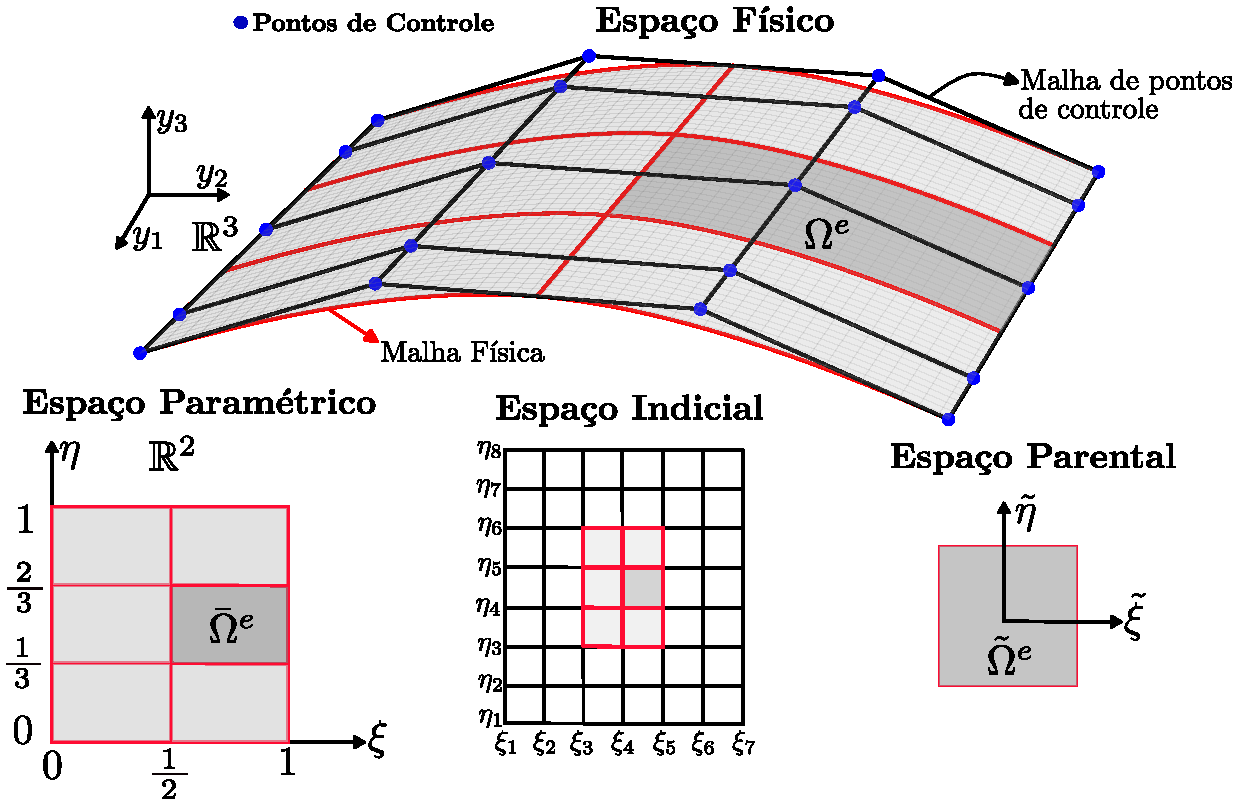
\includegraphics[scale=0.7,trim=0cm 0cm 0cm 0cm, clip=true]{Imagens/Cap3/espacos_NURBS.pdf}	
	\caption{NURBS: espaço físico, espaço paramétrico, espaço indicial e espaço parental}
	\label{fig:espacos_NURBS}
\end{figure}


A malha física representa a geometria discretizada. Dentro da malha física podem ser definidos dois tipos de elementos, um macro-elemento, denominado de \textit{patch}, e o \textit{knot span}, que é o equivalente a um elemento finito e será denominado como célula ao longo desse texto. Cada \textit{patch} é composto por um conjunto de células. Muitas geometrias simples podem ser discretizadas apenas com um \textit{patch}, entretanto, a depender da complexidade da geometria ou de requisitos de parametrização, se torna necessário o uso de um conjunto de \textit{patches}. As células são representações geométricas de linhas, superfícies e volumes nos espaços físicos unidimensional, bidimensional e tridimensional respectivamente.

Cada \textit{patch} e suas respectivas células possuem uma representação ainda no espaço paramétrico (Fig. \ref{fig:espacos_NURBS}), que é o espaço onde as funções base são definidas. O espaço paramétrico, para os casos unidimensionais, é definido por um \textit{knot vector}, aqui denominado de vetor de \textit{knots}, que é um conjunto de \textit{knots} ou coordenadas paramétricas. As células são constituídas pelo espaço entre dois \textit{knots}. O espaço onde se representam todas as células, inclusive as nulas (quando mais de um \textit{knot} ocupa a mesma posição), é chamado de espaço indicial.

Por fim, na análise isogeométrica conta-se ainda com o espaço parental, que é o espaço de integração numérica das funções base, em geral, definido de forma adimensional $[-1, 1]$ dentro de um elemento. Na Fig. \ref{fig:espacos_NURBS} pode-se observar os espaços relatados para uma superfície 3D construída por funções base quadráticas e apenas um \textit{patch}. 

\section{Representação geométrica utilizando \newline{NURBS}} \label{capitulo:Cap3:RepreGeo}´

\subsection{\textit{B-Splines}}

Para a construção de uma geometria NURBS, é fundamental compreender as funções base \textit{B-splines} e suas particularidades. Essas funções servem como o ponto de partida para a definição de curvas, superfícies e sólidos NURBS, sendo essenciais para o entendimento da flexibilidade e controle geométrico oferecido por esse modelo. As \textit{B-splines} são funções \textit{spline} que dependem de um conjunto de pontos de controle e de um vetor de coordenadas paramétricas (vetor de \textit{knots}), os quais determinam a forma e a continuidade da geometria.


\subsubsection{Vetor de \textit{knots}}

As funções \textit{B-Splines}, utilizadas na construção das NURBS, são definidas em um espaço paramétrico que é comum a um conjunto de células ou \textit{patch}. O espaço paramétrico unidimensional é construído através de um vetor de \textit{knots}, que consiste em um conjunto não decrescente de coordenadas paramétricas, definido como: $\Xsi=\left[\xsi_{0},\xsi_{1},...,\xsi_{n+p+1}\right]$,  sendo que $\xsi_{i}\in \realspace$ e representa a coordenada paramétrica do \textit{knot} $i$ com $i = 0, 1, ..., n+p+1$, $n$ é o número de funções base nesta direção paramétrica e $p$ o seu grau polinomial. Os \textit{knots} definem células no espaço paramétrico, cujos contornos são mapeados pelas funções base para formar a malha no espaço físico. 

O vetor de \textit{knots} pode ser classificado como uniforme, quando as coordenadas paramétricas são igualmente espaçadas, e como não-uniformes, caso contrário.
A multiplicidade de um \textit{knot} pode ser superior a um, influenciando diretamente na continuidade e na forma das funções base, conforme será visto posteriormente.  Os vetores de \textit{knots} conhecidos como abertos, são frequentemente utilizados nas literaturas de CAD, e caracterizam-se por ter a primeira e a última coordenada paramétrica repetidas $p+1$ vezes. Este fato garante que as funções sejam interpolatórias nos extremos do espaço paramétrico e nas bordas entre \textit{patches}, proporcionando, por exemplo, a homogeneidade com respeito às condições de contorno essenciais. 

\subsubsection{Funções base e suas derivadas}

As funções base \textit{B-Splines} univariadas são definidas a partir de um vetor de \textit{knots}, sendo para $p=0$, escritas através da seguinte relação:

\begin{align}
\Nb_{i,0}(\xsi) = \begin{cases} 1 &\mbox{if } \xsi_i\leq\xsi<\xsi_{i+1} \\
0 & \mbox{caso contrário } \end{cases}, \label{eq:bsplines_0}
\end{align}

\noindent enquanto que para funções com $p\geq1$ são definidas como:

\begin{align}
\Nb_{i,p}(\xsi)=\frac{\xsi-\xsi_{i}}{\xsi_{i+p}-\xsi_{i}}\Nb_{i,p-1}(\xsi) + 
\frac{\xsi_{i+p+1}-\xsi}{\xsi_{i+p+1}-\xsi_{i+1}}\Nb_{i+1,p-1}(\xsi). \label{eq:bsplines_n}
\end{align}


Essas equações são conhecidas como a fórmula recursiva de \textit{Cox-de Boor} \cite{Cox1972,DEBOOR1972}. Para funções B-Spline de grau $p=0$ ou $p=1$, obtêm-se, respectivamente, as mesmas funções constantes e lineares por partes utilizadas no método dos elementos finitos padrão.

Na Fig.\ref{fig:bspline_funcoes}, pode-se observar funções \textit{B-Splines} quadráticas construídas sobre o vetor de \textit{knots} não-uniforme aberto $\Xsi=\left[0,0,0,1,2,3,3,4,4,4\right]$. A figura evidencia que, devido à repetição de $p+1$ ocorrências dos \textit{knots} nas extremidades do vetor, as funções base se tornam interpolatórias nesses pontos. Ademais, a presença de um \textit{knot} com multiplicidade 2 em $\xsi=3$ reduz a regularidade da função base nesse ponto, resultando na descontinuidade da sua derivada. Em termos gerais, a continuidade de uma função \textit{B-Spline} em uma coordenada paramétrica é dada por $C^{p-m}$, onde $m$ é a multiplicidade do \textit{knot}.

\begin{figure}[htb!]
	\centering 
	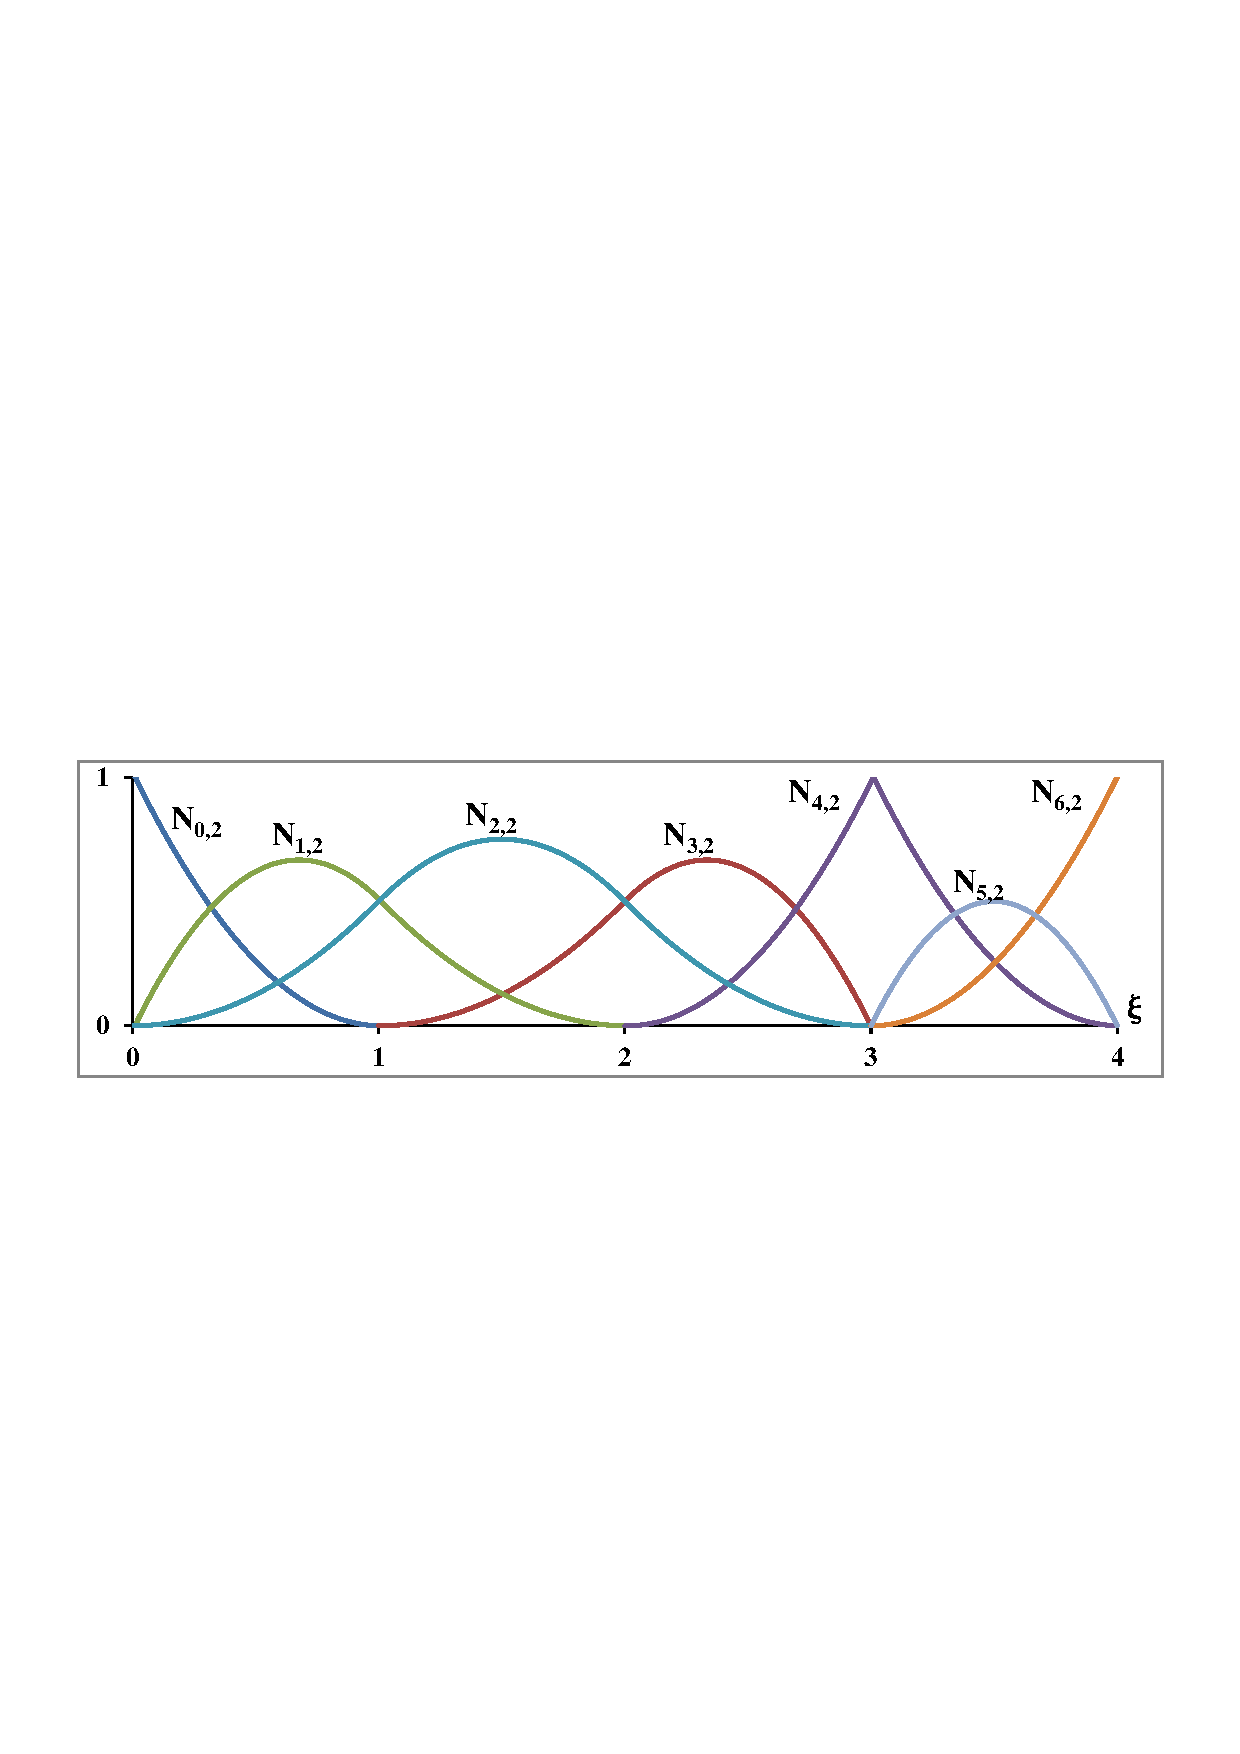
\includegraphics[scale=0.7,trim=1.5cm 11.5cm 1.5cm 13cm, clip=true]{Imagens/Cap3/bspline_funcoes.pdf}	
	\caption{\textit{B-Splines quadráticas}}
	\label{fig:bspline_funcoes}
\end{figure}

As principais propriedades das funções \textit{B-Splines} são:

\begin{itemize}
	\item \textbf{Partição da Unidade}: $\sum_{i=0}^{n}\Nb_{i,p}(\xsi)=1 $;
	\item \textbf{Positividade}: Todas as funções base são positivas, ou seja, $\Nb_{i,p}\geq0$, $\forall\xsi$;
	\item \textbf{Suavidade}: função de ordem $p$ é, em geral, $p-1$ vezes continua no contorno das células;
	\item \textbf{Suporte Compacto}: O suporte de cada $\Nb_{i,p}$ está contido no intervalo $\left[\xsi_i,\xsi_{i+p+1}\right]$, ou seja, em cada célula, apenas $p+1$ funções são não nulas. % Deve-se notar no entanto que, ao se extenderem por vários elementos, o suporte é menos compacto do que para bases formadas por polinômios de lagrange definidos em elementos finitos.
\end{itemize}

A derivada de uma função de forma \textit{B-Spline} pode ser calculada recursivamente em termos de funções base de ordem menor. Considerando uma função de ordem $p$ e vetor de \textit{knots} $\Xsi$, a derivada da i-ésima função de forma pode ser escrita como:

\begin{align}
\frac{\deriv}{\deriv \xsi} \Nb_{i,p}(\xsi) = \frac{p}{\xsi_{i+p} - \xsi_{i}}\Nb_{i,p-1}(\xsi) - \frac{p}{\xsi_{i+p+1} - \xsi_{i+1}}\Nb_{i+1,p-1}(\xsi).
\end{align}

Essa expressão pode ser generalizada para derivadas de ordem superior através de:

\begin{align}
	\frac{\deriv^{k}}{\deriv^{k} \xsi} \Nb_{i,p}(\xsi) = \frac{p!}{\left(p-k\right)!} \sum_{j=0}^{k}{\alpha_{k,j}\Nb_{i+j,p-k}(\xsi)},
\end{align}

sendo $k$ a k-ésima derivada da função $\Nb_{i,p}(\xsi)$ e:

\begin{align}
	\alpha_{0,0} = 1,
\end{align}
\begin{align}
	\alpha_{k,0} = \frac{\alpha_{k-1,0}}{\xsi_{i+p-k+1}-\xsi_{i}},
\end{align}
\begin{align}
	\alpha_{k,j} = \frac{\alpha_{k-1,j}-\alpha_{k-1,j-1}}{\xsi_{i+p+j-k+1}-\xsi_{i+j}} \ \ j=1,...,k-1,
\end{align}
\begin{align}
	\alpha_{k,k} = \frac{-\alpha_{k-1,k-1}}{\xsi_{i+p+1}-\xsi_{i+k}}.
\end{align}

Algoritmos eficientes para a determinação das funções de forma \textit{B-Splines} e de suas derivadas podem ser encontradas em \citeonline{PiegT:1996}.

\subsubsection{Geometrias \textit{B-Splines}}

Uma curva \textit{B-Spline} é construída a partir da combinação linear entre funções base e um conjunto de pontos de controle. Considerando um conjunto de $n$ funções base $\Nb_{i,p}$ e respectivos pontos de controle $\CP_i$ $\in \nrealspace$ com $i = 0,1,...,n$,
uma curva polinomial por partes \textit{B-Spline} unidimensional é definida como:

\begin{align}
\mathbf{C} =\pos\left(\xsi\right) = \sum_{i=0}^{n}\Nb_{i,p}(\xsi)\CP_i,
\end{align}

\noindent com $y_1$, $y_2$ e $y_3$ sendo as coordenadas físicas de um espaço cartesiano. Utilizando as funções \textit{B-Splines} apresentadas na Fig.\ref{fig:bspline_funcoes} e uma malha de pontos de controle qualquer, obtém-se a curva apresentada na Fig.\ref{fig:bspline_malhaPC}. Na Fig.\ref{fig:bspline_curva} pode-se observar as células físicas equivalentes a essa combinação.

\begin{figure}[!htb]
	\centering	
	\subfloat[Malha de pontos de controle\label{fig:bspline_malhaPC}]{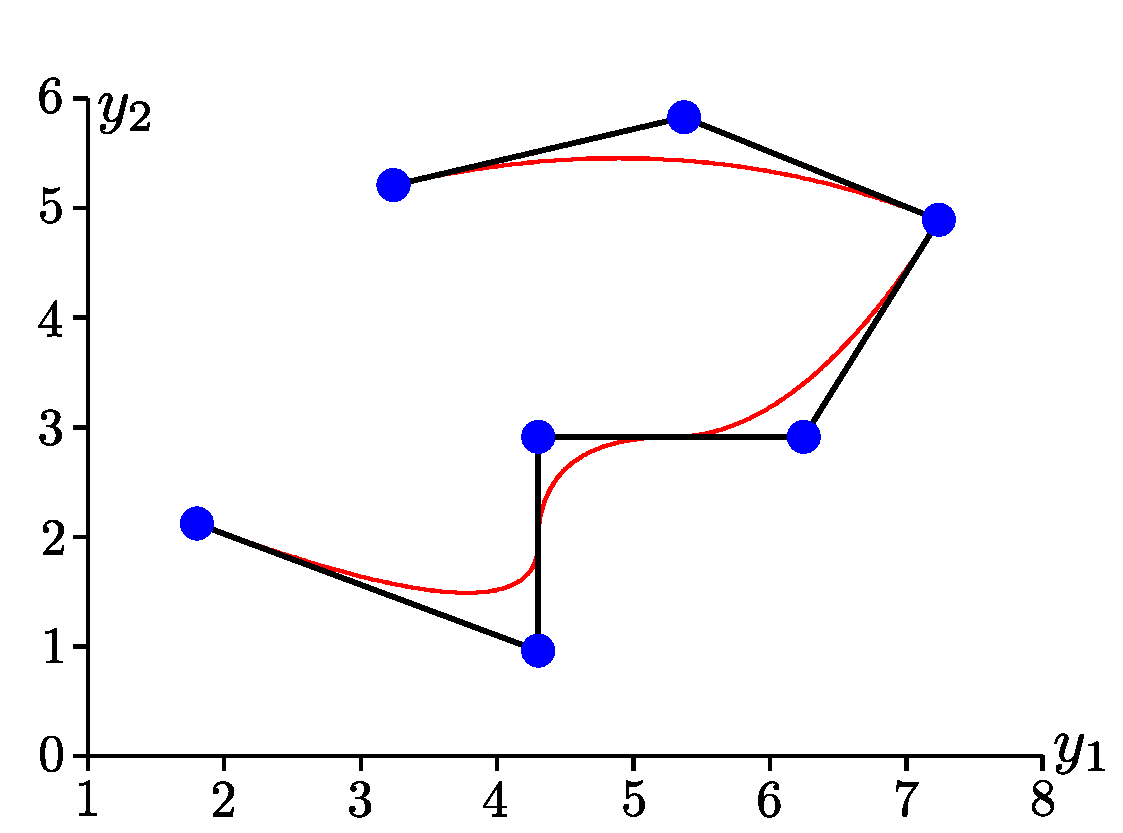
\includegraphics[scale=0.4,trim=0cm 0.0cm 0cm 0cm, clip=true]{Imagens/Cap3/bspline_malhaPC.pdf}} \ \ 
	\subfloat[Curva \textit{B-spline} e representação física das células \label{fig:bspline_curva}]{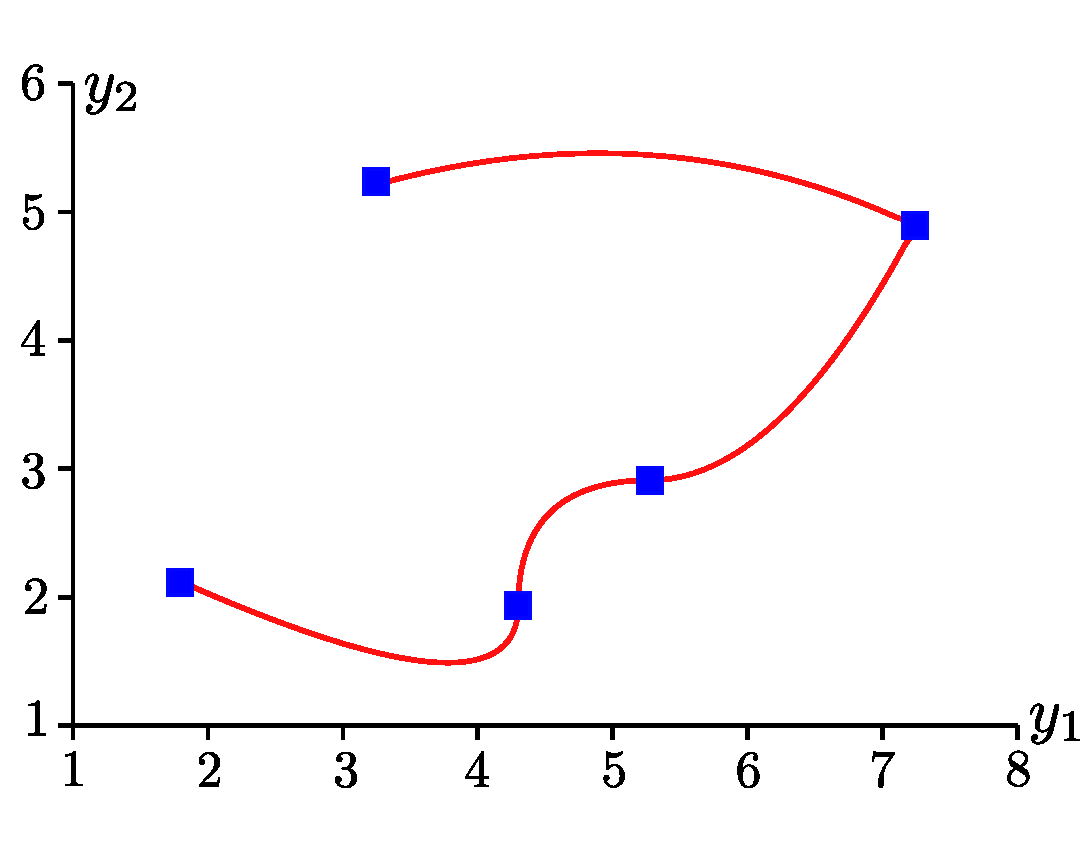
\includegraphics[scale=0.4,trim=0cm 0.7cm 0cm 0cm, clip=true]{Imagens/Cap3/bspline_curva.pdf}}
	\caption{Curva \textit{B-Spline}}
\end{figure}

A partir da Fig.\ref{fig:bspline_curva} pode-se constatar que a curva \textit{B-Spline} interpola o primeiro e o último ponto de controle, que é uma característica das curvas construídas com funções descritas a partir de vetores de \textit{knots} abertos. Adicionalmente nota-se que, devido à multiplicidade do \textit{knot} de coordenada paramétrica $\xsi=3$, existe um ponto de controle intermediário também interpolando a curva. 
Coordenadas paramétricas com multiplicidade maior ou igual ao grau polinomial $p$ resultam, por definição, em interpolação dos pontos de controle associados.
Além disso, a curva possui continuidade $C^{p-1} = C^{1}$ em todos os lugares, exceto em $\xsi = 3$, onde equivale a $C^{p-2} = C^{0}$, que trata-se de uma propriedade herdada das funções base.

Conforme observado  Fig.\ref{fig:bspline_curva}, muitas das características de curvas \textit{B-Splines} são consequências das propriedades das funções \textit{B-splines}. Outra importante propriedade dessas curvas é a Transformação Afim, que significa que uma transformação afim de uma curva B-spline é obtida aplicando a transformação diretamente aos pontos de controle. Além disso, devido ao suporte compacto das funções base, as curvas \textit{B-Splines} possuem característica denominada de \textit{localidade}, que significa que, movendo-se um ponto de controle, afeta-se não mais do que $p+1$ células na curva. Outras propriedades matemáticas das curvas \textit{B-Splines} podem ser consultadas em detalhes em \citeonline{PiegT:1996}.

Uma superfície \textit{B-spline} é obtida analogamente à curva \textit{B-spline}. Dado uma rede de pontos de controle $\CP_{i,j}$ $\in \nrealspace$ com $i = 0,1,...,n$ e $j = 0,1,..., m$, e vetores de \textit{knots} $\Xsi = \left[\xsi_{0},\xsi_{1},...,\xsi_{p+n+1}\right]$, $\mathcal{H} = \left[\eta_{0},\eta_{1},...,\eta_{q+m+1}\right]$, a superfície é obtida através do produto tensorial entre $n$ funções univariadas $\Nb_{i,p}$ e $m$ funções univariadas $\Mb_{j,q}$ da seguinte forma:

\begin{align}
\mathbf{S} = \pos\left(\xsi,\eta\right)  = \sum_{i=0}^{n}\sum_{j=0}^{m}\Nb_{i,p}(\xsi)\Mb_{j,q}(\eta)\CP_{i,j},
\end{align}

\noindent onde $q$ representa o grau das funções na direção paramétrica $\eta$. 
Muitas das propriedades das superfícies B-Splines são resultado da natureza do produto tensorial que as geram. A base de funções apresenta propriedade de positividade e formam uma partição de unidade, de forma que: $\forall(\xsi,\eta)$ $in \left[\xsi_{0},\xsi_{1},...,\xsi_{p+n+1}\right] \times  \left[\eta_{0},\eta_{1},...,\eta_{q+m+1}\right]$:

\begin{align}
 \sum_{i=0}^{n}\sum_{j=0}^{m}\Nb_{i,p}(\xsi)\Mb_{j,q}(\eta) = \left(\sum_{i=0}^{n} \Nb_{i,p}(\xsi)\right) \left(\sum_{j=0}^{m} \Mb_{j,q}(\eta)\right) = 1.
\end{align}

O suporte, por exemplo, de uma função bivariada $\hat{\Nb}_{i,j:p,q}\left(\xsi,\eta\right) = \Nb_{i,p}(\xsi)\Mb_{j,q}(\eta)$ é equivalente à: $\left[\xsi_{i},\xsi_{i+p+1}\right]\times\left[\eta_{j},\eta_{j+q+1}\right]$.

Por fim, um sólido \textit{B-Spline} é obtido através do produto tensorial entre funções univariadas $\Nb_{i,p}$, $\Mb_{j,q}$, $\Lb_{k,r}$, construídas sobre os vetores de \textit{knots} $\Xsi = \left[\xsi_{0},\xsi_{1},...,\xsi_{p+n+1}\right]$, $\mathcal{H} = \left[\eta_{0},\eta_{1},...,\eta_{q+m+1}\right]$ e $\mathcal{Z} = \left[\zeta_{0},\zeta_{1},...,\zeta_{l+r+1}\right]$ respectivamente, e um conjunto de pontos de controle  $\CP_{i,j,k}$ $\in \nrealspace$ com $i = 0,1,...,n$, $j = 0,1,..., m$, $k = 0,1,..., r$, da seguinte forma:

\begin{align}
\mathbf{T} = \pos\left(\xsi,\eta,\zeta\right)  = \sum_{i=0}^{n}\sum_{j=0}^{m}\sum_{k=0}^{l}\Nb_{i,p}(\xsi)\Mb_{j,q}(\eta)\Lb_{k,r}(\zeta)\CP_{i,j,k},
\end{align}

\noindent na qual $l$ e $r$ representam o número de funções e o grau das funções na direção paramétrica $\zeta$. As propriedades de um sólido \textit{B-Spline}, correspondem às generalizações trivariadas das propriedades das superfícies \textit{B-Spline}. Além disso, o suporte de uma função trivariada $\hat{\Nb}_{i,j,k:p,q,r}\left(\xsi,\eta,\zeta\right) = \Nb_{i,p}(\xsi)\Mb_{j,q}(\eta)\Lb_{k,r}(\zeta)$ está contido no intervalo $\left[\xsi_{i},\xsi_{i+p+1}\right]\times\left[\eta_{j},\eta_{j+q+1}\right]\times\left[\zeta_{k},\zeta_{k+r+1}\right]$.


\subsubsection{Refinamento}

Um dos aspectos mais relevantes das \textit{B-splines} é a flexibilidade na forma de enriquecimento da base, permitindo aprimorar sua representação sem alterar a geometria subjacente nem sua parametrização. Dentre os principais procedimentos utilizados, destacam-se: a inserção de \textit{knots} (ou refinamento $h$), que consiste na subdivisão da malha; a elevação de grau (ou refinamento $p$), que aumenta a ordem polinomial das funções base; o refinamento $k$, que promove simultaneamente um aumento da ordem e da continuidade entre elementos; e, por fim, o refinamento $hpk$, que combina de forma coordenada as três estratégias anteriores, oferecendo maior controle e eficiência na representação da geometria e na solução numérica de problemas.

Neste trabalho, será adotado na geração das geometrias o refinamento $h$, baseado na inserção de \textit{knots}. Por essa razão, somente essa estratégia será abordada ao longo desse texto.

O enriquecimento das funções base utilizando a inserção de \textit{knots} é realizado sem que se altere uma curva geometricamente ou parametricamente. Para essa finalidade, considerando o vetor de \textit{knots} $\Xsi = [\xsi_1,\xsi_2, ..., \xsi_{n+p+1}]$, será introduzido o conceito de vetor de \textit{knots} estendido, o qual compreende em: $\bar{\Xsi} = [\bar{\xsi_1} = \xsi_1,\bar{\xsi_2}, ..., \bar{\xsi_{n+m+p+1}}= \xsi_{n+p+1}]$. As $n+m$ novas funções de base \textit{B-Splines} são determinadas através da Eq. \ref{eq:bsplines_0} e Eq. \ref{eq:bsplines_n} aplicando-as ao vetor de \textit{knots} $\bar{\Xsi}$. Os $n+m$ novos pontos de controle  $\bar{\mathcal{B}} = [\bar{\CP}_0,\bar{\CP}_1,..., \bar{\CP}_{n+m}]^{T}$ são obtidos através da combinação linear dos $n$ pontos de controle originais, $\mathcal{B} = [\CP_0,\CP_1,..., \CP_{n}]^{T}$, por:


\begin{align}
	\bar{\mathcal{B}} = \mathbf{T}^{p}\mathcal{B},
\end{align}

\noindent, com:

\begin{align}
	\mathbf{T}_{ij}^{0} = \begin{cases} 1 &\mbox{if } \bar{\xsi}_i \in \left[\xsi_j,\xsi_{j+1}\right) \\
		0 & \mbox{caso contrário } \end{cases}, 
\end{align}

\noindent e:

\begin{align}
	\mathbf{T}_{ij}^{q+1} = \frac{\bar{\xsi}_{i+q}-\xsi_j}{\xsi_{j+q}-\xsi_j}\mathbf{T}_{ij}^{q} + \frac{\xsi_{j+q+1}-\bar{\xsi}_{i+q}}{\xsi_{j+q+1}-\xsi_{j+1}}\mathbf{T}_{ij+1}^{q} \text{com} q=0,1,2,...,p-1.
\end{align}

Considerando uma curva quadrática \textit{B-spline} construída sobre um vetor de \textit{knots} aberto $\Xsi=[0,0,0,1,1,1]$ apresentada na Fig. \ref{fig:bspline_pc_ai} juntamente com sua rede de pontos de controle. Essa curva, possui apenas um elemento no espaço físico, conforme pode ser observado na Fig. \ref{fig:bspline_curva_ai}, e $3$ funções base no espaço paramétrico (Fig. \ref{fig:bspline_base_ai}). Ao realizar-se a inserção de um \textit{knot}, $\xsi=1/2$, o vetor de \textit{knots} estendido fica definido como: $\bar{\Xsi}=[0,0,0,1/2,1,1,1]$. Aplicando-se as Eq. \ref{eq:bsplines_0} e Eq. \ref{eq:bsplines_n} à esse vetor de coordenadas paramétricas, obtém-se as $4$ funções base apresentadas na Fig.\ref{fig:bspline_base_di} definidas sobre 2 células do espaço paramétrico. Após o emprego do refinamento $h$, a geometria da curva é preservada. No entanto, como ilustrado na Fig. \ref{fig:bspline_curva_di}, uma nova célula física é inserida, além de que, de acordo com a Fig. \ref{fig:bspline_pc_di}, a malha de pontos de controle é modificada, com o acréscimo um novo ponto e o reajuste de suas posições.


\begin{figure}[!t]
	\centering
	\subfloat[\label{fig:bspline_pc_ai}Curva original e pontos de pontrole]{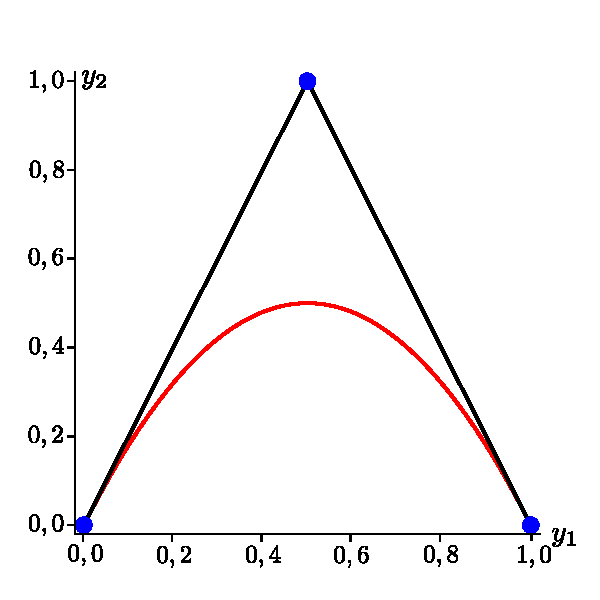
\includegraphics[scale=0.7,trim=0cm 0cm 0cm 1cm, clip=true]{Imagens/Cap3/bspline_pc_ai.pdf}} 
	\subfloat[\label{fig:bspline_pc_di}Curva refinada e pontos de controle]{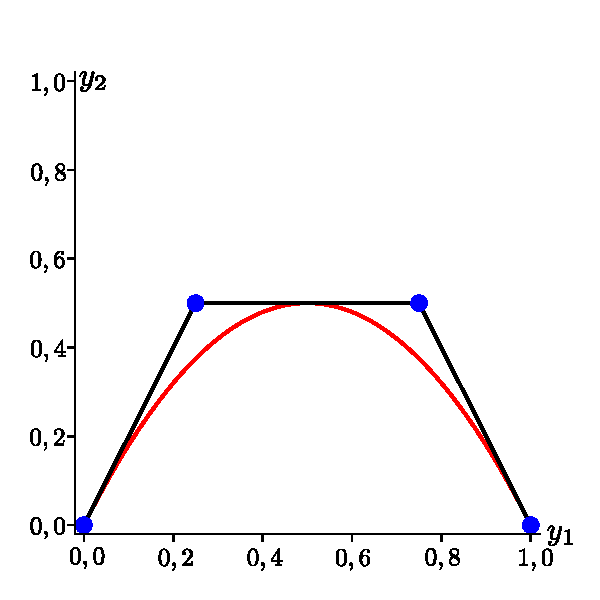
\includegraphics[scale=0.7,trim=0cm 0cm 0cm 1cm, clip=true]{Imagens/Cap3/bspline_pc_di.pdf}} \\ 
	\subfloat[\label{fig:bspline_curva_ai}Elementos curva original]{\includegraphics[scale=0.7,trim=0cm 0cm 0cm 1cm, clip=true]{Imagens/Cap3/bspline_curva_ai.pdf}} 
	\subfloat[\label{fig:bspline_curva_di}Elementos curva refinada]{\includegraphics[scale=0.7,trim=0cm 0cm 0cm 1cm, clip=true]{Imagens/Cap3/bspline_curva_di.pdf}} \\ 
	\subfloat[\label{fig:bspline_base_ai}Funções base originais]{\includegraphics[scale=0.7,trim=0cm 0cm 0cm 0.5cm, clip=true]{Imagens/Cap3/bspline_base_ai.pdf}} 
	\subfloat[\label{fig:bspline_base_di}Funções base após refinamento $h$ refinada]{\includegraphics[scale=0.7,trim=0cm 0cm 0cm 0.5cm, clip=true]{Imagens/Cap3/bspline_base_di.pdf}} 
	\caption{Refinamento $h$ para um curva \textit{B-Spline}}
	\label{fig:bspline_insercaoKnots}
\end{figure}


\subsection{\textit{B-Splines} não-uniformes racionais e análise isogeométrica}

Uma entidade NURBS no $\realspace^{d}$ pode ser entendida, de ponto de vista geométrico, como a projeção transformativa de uma entidade \textit{B-Spline} no $\realspace^{d+1}$. Geometrias cônicas podem ser construídas exatamente pela projeção transformativa de curvas por partes quadráticas (para maiores detalhes sobre projeção transformativa, ver \citeonline{Farin:1999}). Na Fig. \ref{fig:circunferencia}, apresenta-se uma curva NURBS $\mathbf{C}\left(\xsi\right)$, que representa, de forma exata, uma circunferência, sendo essa obtida a partir da projeção de uma curva \textit{B-Spline} $\mathbf{C}^{w}\left(\xsi\right)$.

\begin{figure}[htb!]
	\centering 
	\includegraphics[scale=0.3,trim=0cm 0cm 0cm 0cm, clip=true]{Imagens/Cap3/transformacaoprojetiva.png}	
	\caption{Projeção transformativa para obtenção circunferência. Fonte: \citeonline{CottrelHB:2009}}
	\label{fig:circunferencia}
\end{figure}

Matematicamente, uma função NURBS é obtida pela racionalização de uma função \textit{B-Spline}. A racionalização dessa função ocorre através da razão entre dois polinômios. Uma função racional NURBS $\left(R\right)$ é construída através da seguinte expressão:

\begin{align}
R_{i}^{p}(\xsi) = \frac{N_{i,p}(\xsi)w_i}{\sum_{\hat{i}=0}^{n}N_{\hat{i},p}(\xsi)w_{\hat{i}}}
\end{align}

\noindent onde $w_i$ e $w_{\hat{i}}$ $\in \realspace$, com $i = \hat{i} =  0, 1, ... , n$ , correspondem aos pesos relativos as funções $N_{i,p}\left(\xsi\right)$ e $N_{\hat{i},p}\left(\xsi\right)$ respectivamente. 

A $d$-ésima derivada de $R_{i}$ (onde suprimiu-se o índice $p$ para facilitar a representação), é obtida da seguinte forma:

\begin{align}
R_{i}^{d}(\xsi) = \frac{N_{i}^{d}(\xsi)w_i - \sum_{l=1}^{d}\left[\binom{d}{l}\sum_{j=1}^{n}N_{j}^{l}(\xsi)w_{j}R_{i}^{d-l}(\xsi)\right]}{\sum_{{j}=0}^{n}N_{{j}}(\xsi)w_{{j}}},
\end{align}

\noindent em que:
\begin{align}
\binom{d}{l} = \frac{d!}{l!\left(d-l\right)!}.
\end{align}

Uma curva NURBS é obtida por:

\begin{align}
\mathbf{C} = \pos\left(\xsi\right) = \sum_{i=0}^{n}R_{i}^{p}(\xsi)\CP_i, \label{eq:curveNURBS}
\end{align}

\noindent sendo os pesos selecionados de maneira a se obter a geometria desejada. Analogamente uma superfície NURBS é obtida através das seguintes relações:

\begin{align}
R_{i,j}^{p,q}(\xsi,\eta) = \frac{N_{i,p}(\xsi)M_{j,q}(\eta)w_{i,j}}{\sum_{\hat{i}=0}^{n}\sum_{\hat{j}=0}^{m}N_{\hat{i},p}(\xsi)M_{\hat{j},q}(\eta)w_{\hat{i},\hat{j}}},
\end{align}

\begin{align}
\mathbf{S} = \pos\left(\xsi,\eta\right) = \sum_{i=0}^{n}\sum_{j=0}^{m}R_{i,j}^{p,q}(\xsi,\eta)\CP_{i,j}, \label{eq:surfaceNURBS}
\end{align}

\noindent com $w_{i,j}$ e $w_{\hat{i},\hat{j}}$ $\in \realspace$, sendo $i = \hat{i} =  0, 1, ... , n$ e  $j = \hat{j} =  0, 1, ... , m$ , correspondem aos pesos relativos às funções $\left(N_{i,p}\left(\xsi\right)M_{j,q}\left(\eta\right)\right)$ e $\left(N_{\hat{i},p}\left(\xsi\right)M_{\hat{j},q}\left(\eta\right)\right)$ respectivamente. Por fim, um sólido NURBS é obtido por:

\begin{align}
R_{i,j,k}^{p,q,r}(\xsi,\eta,\zeta) = \frac{N_{i,p}(\xsi)M_{j,q}(\eta)L_{k,r}(\zeta)w_{i,j,k}}
{\sum_{\hat{i}=0}^{n}\sum_{\hat{j}=0}^{m}\sum_{\hat{k}=0}^{l}N_{\hat{i},p}(\xsi)M_{\hat{j},q}(\eta)L_{\hat{k},r}(\zeta)w_{\hat{i},\hat{j},\hat{k}}},
\end{align}

\begin{align}
\mathbf{T} = \pos\left(\xsi,\eta,\zeta\right) = \sum_{i=0}^{n}\sum_{j=0}^{m}\sum_{k=0}^{l}R_{i,j,k}^{p,q,r}(\xsi,\eta,\zeta)\CP_{i,j,k}, \label{eq:solidNURBS}
\end{align}

\noindent onde $w_{i,j,k}$ e $w_{\hat{i},\hat{j},\hat{k}}$ $\in \realspace$, sendo $i = \hat{i} =  0, 1, ... , n$, $j = \hat{j} =  0, 1, ... , m$ e $k = \hat{k} =  0, 1, ... , l$, correspondem aos pesos relativos às funções $\left(N_{i,p}\left(\xsi\right)M_{j,q}\left(\eta\right)L_{k,r}\left(\zeta\right)\right)$ e $(N_{\hat{i},p}\left(\xsi\right)M_{\hat{j},q}\left(\eta\right)L_{\hat{k},r}\left(\zeta\right))$ respectivamente.

Na aplicação da IGA, as funções tentativa para velocidade e pressão, e as funções peso associadas a elas, apresentadas nas Eq. \eqref{eq:vel} à Eq. \eqref{eq:ptest} como $N$, são equivalentes à $R_{i}^{p}(\xsi)$, $R_{i,j}^{p,q}(\xsi,\eta)$ e $R_{i,j,k}^{p,q,r}(\xsi,\eta,\zeta)$ para os casos unidimensional, bidimensional e tridimensional respectivamente. E a geometria é representada pelas Eq. \eqref{eq:curveNURBS}, Eq. \eqref{eq:surfaceNURBS} e Eq. \eqref{eq:solidNURBS} dependendo da dimensão do problema em análise. 

A integração numérica nas células é realizada através da quadratura Gaussiana. Considerando o domínio paramétrico de uma célula $\tilde{\domain}^{e}$ e o domínio parental $\hat{\domain}^{e}$  apresentados na Fig.\ref{fig:espacos}, definidos respectivamente em um espaço tridimensional pelas coordenadas $\coordAdimen\left(\xsi,\eta,\zeta\right)$ e $\hat{\coordAdimen}(\hat{\xsi},\hat{\eta},\hat{\zeta})$, a matriz jacobiana do mapeamento do espaço físico, com coordenadas $\mathbf{x} \left(x,y,z\right)$,  para o espaço de quadratura, é definida por:

\begin{align}
\frac{d\pos}{d\hat{\coordAdimen}} = \frac{d\pos}{d\coordAdimen} \frac{d\coordAdimen}{d\hat{\coordAdimen}} \label{eq:integ}
\end{align}

O primeiro termo à direita da igualdade da Eq. \eqref{eq:integ} é calculado a partir das derivadas de Eq. \eqref{eq:curveNURBS}, Eq. \eqref{eq:surfaceNURBS} e Eq. \eqref{eq:solidNURBS} e o segundo termo, considerando a célula $\tilde{\domain}^{e} = [\xsi_{i},\xsi_{i+1}] \times [\eta_{j},\eta_{j+1}] \times [\zeta_{k},\zeta_{k+1}]$, calcula-se $\xsi,\eta, \zeta$ $\in \tilde{\domain}^{e}$ a partir de $\hat{\xsi},\hat{\eta}, \hat{\zeta}$ $\in \hat{\domain}^{e}$ através das seguintes relações: 


\begin{align}
\xsi = \xsi_{i} + \left(\hat{\xsi}+1\right) \left(\frac{\xsi_{i+1}-\xsi_{i}}{2}\right),
\end{align}

\begin{align}
\eta = \eta_{i} + \left(\hat{\eta}+1\right) \left(\frac{\eta_{i+1}-\eta_{i}}{2}\right)
\end{align}

\noindent e

\begin{align}
\zeta = \zeta_{i} + \left(\hat{\zeta}+1\right) \left(\frac{\zeta_{i+1}-\zeta_{i}}{2}\right).
\end{align}

\subsection{Parâmetros de estabilização}\label{capitulo:Cap3:RepreGeo:taus2}

Considerando que nesse trabalho dois tipos de aproximações espaciais são utilizadas, uma baseada no FEM e outra baseada em IGA, adotam-se os parâmetros propostos por \citeonline{TakizawaTO:2018} e \citeonline{OtoguroTT:2020}, que são adequados para ambas aproximações. 

Para essa opção é necessário definir-se o tensor métrico do elemento no espaço. Para isso, inicia-se com a definição da matriz Jacobiana $\matrixQ$, dada por:

\begin{align}
	\matrixQ&=\left(\frac{\partial\pos}{\partial\coordAdimen}\right),
\end{align}

\noindent com $\coordAdimen$ representando as coordenadas do espaço paramétrico. Para que a ordem polinomial seja levada em consideração na determinação dos parâmetros de estabilização, aplica-se uma mudança de escala na matriz $\matrixQ$, através da matriz $\matrixD$, conforme a seguinte expressão:

\begin{align}
	\matrixQhat&=\matrixQ\matrixD^{-1}.
\end{align}

Para elementos finitos com funções de forma polinomiais Lagrangianas de ordem $p_i$, definidas na direção $i$ do espaço paramétrico, com $-1\leq\xsi_i\leq1$, a matriz $\matrixD$ é definida como:

\begin{align}
	\matrixD&=\begin{bmatrix}
		p_{1} & 0 & 0\\
		0 & p_{2} & 0 \\
		0 & 0 & p_{3}
	\end{bmatrix}.
\end{align}


Para discretização utilizando IGA adota-se:

\begin{align}
	\matrixD&=\left(\frac{\partial\bar{\coordAdimen}}{\partial\coordAdimen}\right),
\end{align}

\noindent com $\bar{\coordAdimen}$ representando as coordenadas do chamado espaço paramétrico preferido. 

Para problemas em 1D, $\matrixD$ é definido como:

\begin{align}
	D&=\frac{\Delta\bar{\coordAdimen}}{\min_{a=1,...,p} \Delta\coordAdimen_{a}},
\end{align}

\noindent onde $\Delta\bar{\coordAdimen}$ é o comprimento do elemento de Bézier no espaço paramétrico (espaço preferido), $p$ é o grau polinomial das funções base e $\Delta\coordAdimen_{a}$ é:

\begin{align}
	\Delta\coordAdimen_{a}&=\frac{\Delta\bar{\coordAdimen}}{p}\sum_{b=0}^{p} \left({\matrixCinv}_{ba} - \matrixCinv_{ba-1}\right),
\end{align}

\noindent a matriz $\matrixCinv$ é o tensor de transformação de Bézier. Para múltiplas dimensões têm-se $\matrixD_{ij} = D^i \delta_{ij} $, com $D^i$ o valor de $D$ na direção $i$.

A partir disso, o comprimento direcional do elemento é definido como:

\begin{align}
	\RQD &=2\left(\rRGN\rRGN : \matrixG \right)^{-\frac{1}{2}},
\end{align}

\noindent sendo $\rRGN$ o vetor direção unitário da velocidade no elemento e $\matrixG$ uma matriz auxiliar, os quais são representados respectivamente como:

\begin{align}
	\rRGN&=\frac{\nabla \lVert\velocityh - \velocityALEh\rVert}{\lVert \nabla \lVert\velocityh - \velocityALEh\rVert\rVert} \label{eq:erRGN}
\end{align}

\noindent e

\begin{align}
	\matrixG &= \matrixQhat^{-T} \cdot \matrixQhat^{-1}. 
\end{align}

O comprimento do elemento é limitado pelos mínimos e máximos valores representados abaixo:

\begin{align}
	h_{min} \equiv 2\min_{r}\left((\rRGN:\matrixG)^{-\frac{1}{2}} \right), \\
	h_{max} \equiv 2\max_{r}\left((\rRGN:\matrixG)^{-\frac{1}{2}} \right).
\end{align}

Os parâmetros de estabilização são dados por:

\begin{align}
	\SUPG = \PSPG =\left(\frac{1}{\SUGNi^2} + \frac{1}{\SUGNii^2} + \frac{1}{\SUGNiii^2} \right)^{-\frac{1}{2}},
\end{align}

\begin{align}
	\LSIC = \frac{\RQD^2}{\SUPG},
\end{align}

\noindent onde:

\begin{align}
	\SUGNi^{-2} = \left(\velocityh - \velocityALEh \right) \left(\velocityh - \velocityALEh \right) : \matrixG ,
\end{align}

\begin{align}
	\SUGNii&=\frac{\Delta t}{2},
\end{align}

\noindent e

\begin{align}
	\SUGNiii^{-1} = \kviscosity \left(\rRGN_{reg}\rRGN_{reg} : \matrixG + \left(1 - \rRGN_{reg}^2)4h_{min}^{-2} \right)\right) ,
\end{align}

\noindent sendo $\rRGN_{reg}$ definido como:

\begin{align}
	\rRGN_{reg} =\frac{\nabla \lVert\velocityh - \velocityALEh\rVert}{\lVert \nabla \lVert\velocityh - \velocityALEh\rVert\rVert + \varepsilon\left(\lVert \nabla \lVert\velocityh - \velocityALEh\rVert\rVert\right)_0},
\end{align}

\noindent com $\varepsilon$ uma constante pequena e $\left(\lVert \nabla \lVert\velocityh- \velocityALEh\rVert\rVert\right)_0$ um valor de referência. Os termos $\SUGNi$, $\SUGNii$ e $\SUGNiii$ são parâmetros correspondentes aos termos convectivos, inerciais e viscosos, respectivamente.

\section{Verificação e aplicações}

Para aplicação da IGA em problemas da DFC seguiu-se o mesmo procedimento matemático descrito ao longo do Cap. \ref{capitulo:Cap1}, sendo que a implementação computacional seguiu o roteiro apresentado no Alg. \ref{alg:fluid_temporalIntegration}. Os exemplos escolhidos para a verificação do código computacional foram o escoamento sobre um cilindro 3D e o problema de escoamento sobre um canal com degrau utilizando células 3D. Os resultados obtidos são apresentados nas seções subsequentes.

\subsection {Escoamento sobre um cilindro - 3D}

Na geração da geometria NURBS, correspondente ao problema do escoamento sobre um cilindro, utilizou-se um código previamente desenvolvido pela estudante durante seu mestrado \cite{Tonon:2016}. Por tratar-se de uma geometria de pequena complexidade, pôde-se gerá-la com um único \textit{patch}, o qual é composto por um cubo com um cilindro inserido em seu centro.
O processo de geração da malha, simplificadamente, consiste em se escolher vetores de $knots$, pontos de controle, e pesos adequados para a descrição de tal geometria.

O código previamente desenvolvido, baseia-se na quantidade mínima de pontos de controle necessários para gerar uma circunferência completa (ver Fig. \ref{fig:pontosdecontroleInicias}). Para a obtenção exata de uma circunferência utilizam-se funções quadráticas e o vetor de \textit {knots} na direção paramétrica $\xsi$ inicial é composto por: $\xsi=\left[0,0,0,1/4,1/4,1/2,1/2,3/4,3/4,1,1,1\right]$. A posição dos pontos de controle da circunferência e seus respectivos pesos foram obtidos de acordo com \citeonline {PiegT:1996}. 

A obtenção da curva respectiva ao quadrado, que é descrita no espaço paramétrico correspondente a direção $\xsi$, é consequência das escolhas realizadas para gerar a circunferência, logo, a curva possui o mesmo vetor de \textit{knots} e funções quadráticas. Os pontos de controle para a formação do quadrado foram posicionados, no espaço físico, de forma a ser obtida a dimensão requerida à seção transversal quadrada que compõe a geometria do cubo, e de forma que os mesmos ficassem alinhados com os pontos de controle da circunferência na direção radial. Os pesos respectivos ao pontos de controle do retângulo são unitários. Na Fig. \ref{fig:pontosdecontroleInicias} pode-se observar a posição dos pontos de controle respectivos à circunferência e ao quadrado e as curvas resultantes desta discretização em linha vermelho pontilhado.

Na sequência o código realiza o procedimento de refinamento por inserção sucessiva de \textit{knots} no vetor de \textit{knots}. O algoritmo utilizado para este procedimento pode ser encontrado em \citeonline {PiegT:1996}. Na Fig. \ref{fig:pontosdecontroleInicias2} apresenta-se um exemplo de pontos de controle gerados após a inserção de um novo \textit{knot} no centro de cada \textit{knot span} do espaço paramétrico inicial. A quantidade de \textit{knots} a ser inserida depende da discretização necessária a análise numérica.

\begin{figure}[!htb]
	\centering	
	\subfloat[Pontos de controle inicias.\label{fig:pontosdecontroleInicias}]{\includegraphics[scale=0.4,trim=1cm 1cm 0.5cm 1cm, clip=true]{Imagens/Cap3/escoamentosobrecilindro.pdf}}
	\subfloat[Pontos de controle após inserção de \textit{knots}.\label{fig:pontosdecontroleInicias2}]{\includegraphics[trim=1cm 1cm 0.5cm 1cm,clip,scale=0.4]{Imagens/Cap3/escoamentosobrecilindro2.pdf}}
	\caption{Cilindro 3D: Geração curva NURBS}
\end{figure}

Para a obtenção de uma seção transversal da geometria em questão, gera-se uma superfície a partir da discretização na direção $\eta$ do espaço paramétrico. O código utiliza um vetor de \textit{knots} aberto, com os 
\textit{knots} distribuídos uniformemente, e funções de forma quadráticas. Os pontos de controle são distribuídos radialmente no espaço físico através de uma progressão geométrica unidirecional e seus pesos são determinados a partir de uma interpolação linear entre os pesos dos pontos de controle da circunferência e os pontos do quadrado. A quantidade mínima de pontos de controle respectiva à direção $\eta$ é de $q+1$ pontos, sendo a quantidade final definida em função da análise numérica. Na Fig. \ref{fig:superficieNURBcilindro}, apresenta-se um exemplo de uma rede de pontos de controle, obtida a partir das curvas apresentadas em Fig. \ref {fig:pontosdecontroleInicias2} com 9 pontos de controle na direção $\eta$. Na figura em questão omitiu-se a nomenclatura dos pontos de controle intermediários às curvas da circunferência e do quadrado para evitar a sobreposição da nomenclatura na figura.


\begin{figure}[htb!]
	\centering 
	\includegraphics[scale=0.4,trim=1cm 1cm 5cm 4cm, clip=true]{Imagens/Cap3/escoamentosobrecilindro3.pdf}	
	\label{fig:superficieNURBcilindro}
	\caption{Cilindro 3D: Geração superfície NURBS.}
\end{figure}

Nessa primeira etapa do trabalho, a direção paramétrica $\zeta$, respectiva à direção $z$ da geometria física, foi discretizada com apenas uma célula, utilizando-se para isso vetor de \textit{knots} abertos com distribuição uniforme de \textit{knots}, e funções base quadráticas.

Visando a verificação do código de IGA 3D analisa-se o problema do escoamento sobre o cilindro para $\Reynolds$ =40 ,100 e 1000 (Eq. \eqref{eq:Reynolds}). Para isso, gera-se uma malha com 101 x 71 x 3 pontos de controle nas direções paramétricas $\xsi$, $\eta$ e $\zeta$ respectivamente, resultando em 6624 células. Na Fig. \ref{fig:cilindrogeometria} apresentam-se as dimensões da geometria em questão, bem como as condições de contorno aplicadas, e na Fig. \ref{fig:cilindromalha} apresenta-se a malha física resultante da discretização.


\begin{figure}[!htb]
	\centering
	\subfloat[\label{fig:cilindrogeometria}Geometria]{\includegraphics[scale=0.48,trim=0cm 0cm 0cm 0cm, clip=true]{Imagens/Cap3/cylinderISO3d.pdf}} 
	\subfloat[\label{fig:cilindromalha} Malha de células físicas]{\includegraphics[scale=0.2,trim=5cm 0cm 0cm 0cm, clip=true]{Imagens/Cap3/malhacilindro.eps}} 
	\caption{Cilindro 3D: Geometria e malha de células físicas}
	\label{fig:cilindro_geoemalha}
\end{figure}

Adicionalmente, prescrevem-se nas paredes frontal e posterior, condição de parede lisa ($u_{z} = 0$), e na \textit{Saída} do escoamento condição de força de superfície nula ($\stressTensor \normal = \mathbf{0}$). O problema é simulado para um velocidade de entrada $u_{\infty} = 1,0$, $\rho = 1,0$, $\timeStep = 0,05$, e $\specRadius = 0,5$, sendo a viscosidade variada de acordo com o número de Reynolds desejado.  Para o cálculo dos coeficientes aerodinâmicos $C_{D}$, $C_{L}$ e do número de Strouhal ($\Strouhal$) utilizam-se as equações apresentadas no Item \ref{subsection:escoamentocil2d}. 

Nas Figs. \ref{fig:cilindro_Cd3d} e \ref{fig:cilindro_Cl3d}, apresentam-se a variação ao longo do tempo dos coeficientes $C_{D}$ e $C_{L}$. Os valores obtidos com a malha isogeométrica 3D estão muito próximos ao obtidos com a malha de elementos finitos 2D (Item \ref{subsection:escoamentocil2d}) para Reynolds 40 e 100. Para Reynolds 1000, nota-se que a variação ao longo do tempo dos valores de $C_{D}$ e $C_{L}$ para IGA resulta em valores mais elevados do que os obtidos com MEF. Tal diferença ainda deverá ser investigada, sendo que tanto as diferenças nas dimensões das malhas como a diferença que pode haver na convergência dos resultados ou a efeitos de 3D de vorticidade podem contribuir para isso. Os resultados obtidos para o histórico de $C_{D}$ e $C_{L}$ por \citeonline{Henderson:1997} para $Re = 1000$ em análises tridimensionais baseadas em MEF, foram menores do que os 2D. Essa disparidade entre os resultados obtidos nesse trabalho e de \citeonline{Henderson:1997} podem estar relacionados com o fato de que a dimensão escolhida da malha na direção $z$ foi muito pequena de maneira a impossibilitar que os efeitos tridimensionais do escoamento fossem adequadamente capturados.

Para o número de Strouhal, o valor obtido para $\Reynolds = 100$ foi de 0,1681 e para $\Reynolds = 1000$ de 0,2395. Nota-se que, embora os valores de $C_{D}$ e $C_{L}$ apresentem diferenças entre os resultados 2d baseados em elementos finitos e a malha 3D baseada em IGA, a frequência do desprendimento de vórtices obtida foi muito semelhante.

\begin{figure}[!htb]
	\centering
	\subfloat[\label{fig:cilindro_Cd3d}Coeficiente de arrasto $ C_D$.]{\includegraphics[scale=0.8,trim=0cm 0cm 0cm 0cm, clip=true]{Imagens/Cap3/DragRe.eps}} 
	\subfloat[\label{fig:cilindro_Cl3d}Coeficiente de sustentação $C_L$.]{\includegraphics[scale=0.8,trim=0cm 0cm 0cm 0cm, clip=true]{Imagens/Cap3/LiftRe.eps}}\\ 
	{\includegraphics[scale=1.3]{Imagens/Cap3/Legenda.pdf}}
	\caption{Cilindro 3D: Coeficientes aerodinâmicos. }
	\label{fig:cilindro_coeficientes3d}
\end{figure}


\subsection {Escoamento em um canal com degrau}

Este exemplo é amplamento utilizado na verificação de códigos para escoamentos incompressíveis, sendo sua geometria apresentada na Fig. \ref{fig:degrau_geo}.  O problema consiste em prescrever-se um perfil parabólico de escoamento na entrada do canal, e condição de aderência ($\velocity = 0$) nas demais paredes que estão contidas nos planos $xz$ e $yz$, exceto na saída do canal, a qual possui como condição $\stressTensor\normal = \mathbf{0}$. Para as paredes dos planos $xy$, frontal e posterior, prescreveu-se condição de parede lisa ($u_{z}=0$). 

\begin{figure}[htb!]
	\centering
	\includegraphics[scale=1.2,trim=0cm 0cm 0cm 0cm, clip=true]{Imagens/Cap3/degrau.pdf}
	\caption{Degrau 3D: Geometria.}
	\label{fig:degrau_geo}
\end{figure}


As dimensões selecionadas para o canal foram $h = 1,0m$, $s = 0,94m$, $x_{e}= 1,0m$, $x_{f}= 15m$ e $x_{t} = 30m$ e dimensão na direção $z$ de $0,1m$. Adicionalmente, o perfil de velocidade na entrada do canal é descrito pela seguinte relação:

\begin{align}
u_{x} = V_{max} \left(1-\left(\frac{\left(y-s\right)-h/2}{h/2}\right)^{2}\right),
\end{align}

\noindent com velocidade $V_{max} = 10 m/s$ e $u_{y} = u_{z} = 0$.

O escoamento sobre o degrau é caracterizado por produzir áreas de recirculação onde o fluido se separa e forma vórtices. A distância entre o degrau e o ponto de recolamento do vórtice principal $x_{r}$ é uma das principais características verificadas nesse problema. A dimensão dos vórtices varia em função do número de $\Reynolds$, a qual é calculada de acordo com \citeonline {ArmalyDP:1983}, sendo expressa por:

\begin{align}
\Reynolds =\frac{\rho\left(\frac{2V_{max}}{3}\right)2h}{\viscosity},
\end{align}

\noindent com $\rho = 1kg/m^{3}$. Foram selecionados para as análises 3 diferentes número de Reynolds: $100$, $400$ e $800$, variando-se a viscosidade do fluido.

Para a geração da geometria NURBS, discretiza-se o canal em 5 \textit{patches}, os quais são denominados $P_{0},P_{1},P_{2},P_{3}$ e $P_{4}$, e podem ser observados na Fig. \ref{fig:degrau_geo}. Todas as direções paramétricas são discretizadas com vetores de \textit{knots} abertos e com \textit{knots} igualmente espaçados no interior do vetor, além de funções de forma quadráticas. Os pontos de controle para os \textit{patches} $0,1$ e $2$ foram distribuídos no espaço físico, direções $x,y$ e $z$ de maneira a se obter células igualmente espaçados. Para os \textit{patches} $3$ e $4$, na direção do espaço físico $y$ e $z$, os pontos são posicionadas de maneira a gerar células uniformes, e, na direção $x$, são distribuídos de maneira a se resultar numa progressão geométrica do tamanho das células, com as células aumentando de tamanho da esquerda para a direita, conforme pode ser observado na Fig. \ref{fig:degrau_malha}. Na Tab. \ref{tab:numberPCpatches} podem ser observados os números de pontos de controle utilizados em cada direção dos espaços paramétricos para cada \textit{patch}, resultando em 60795 pontos de controle e 4800 células.

\begin{figure}[htb!]
	\centering
	\includegraphics[scale=0.3,trim=1cm 14cm 1cm 14cm, clip=true]{Imagens/Cap3/malhadegrau.eps}
	\caption{Degrau 3D: Geometria e malha de células físicas}
	\label{fig:degrau_malha}
\end{figure}

\begin{center}
	\begin{table}[h!]
		\caption{Número de pontos de controle por \textit{patch}}
		\centering
		\begin{tabular}{|c | c | c| c|} 
			\hline
			\textit{Patch} & $\xsi$ & $\eta$ & $\zeta$ \\ 
			\hline
			0 & 22 & 12 & 3 \\ 
			\hline
			1 & 152 & 12 & 3\\
			\hline
			2 & 152 & 12 & 3\\
			\hline
			3 & 82 & 12 & 3\\
			\hline
			4 & 82 & 12 & 3\\
			\hline
		\end{tabular}
		\label{tab:numberPCpatches}
	\end{table}
\end{center}


Na Fig. \ref{fig:degrau_com_recl} são apresentados os comprimentos de recolamento do vórtice primário adimensionalizados ($x_{r}/s$), juntamente com os resultados adaptados dos ensaios experimentais de \citeonline{ArmalyDP:1983} e os resultados de análises 2d de \citeonline{WilliamsB:1999}. Nota-se que os resultados obtidos estão próximos das referências para $\Reynolds = 100$ e $\Reynolds =400$, entretanto, para $\Reynolds = 800$ nota-se um afastamento do presente trabalho, e do referente à análise 2D com relação ao experimento realizado por \citeonline{ArmalyDP:1983}. Isto ocorre, visto que o ensaio experimental foi realizado com um canal com $2m$ de comprimento na direção $z$, e a simulação atual com apenas uma célula nessa direção é incapaz de captar os fenômenos tridimensionais que ocorrem a medida que o número de Reynolds cresce. Na Fig.\ref {fig:degrau_vortices} pode-se observar o campo de velocidade para os Reynolds estudados, e o aspecto do vórtice primário desenvolvido.


\begin{figure}[htb!]
	\centering
	\includegraphics[scale=1.2,trim=0cm 0cm 0cm 0cm, clip=true]{Imagens/Cap3/comvort.eps}
	\caption{Degrau 3D: Comprimento de recolamento do v\'ortice principal}
	\label{fig:degrau_com_recl}
\end{figure}


\begin{figure}[!htb]
	\centering
	\subfloat[\label{fig:vortice_re100} $\Reynolds= 100$]{\includegraphics[scale=0.3,trim=0cm 0cm 0cm 0cm, clip=true]{Imagens/Cap3/degrau100.pdf}} \\
	\subfloat[\label{fig:vortice_re400} $\Reynolds= 400$]{\includegraphics[scale=0.36,trim=0cm 0cm 0cm 0cm, clip=true]{Imagens/Cap3/degrau400.pdf}}\\ 
	\subfloat[\label{fig:vortice_re800}$\Reynolds= 800$]{\includegraphics[scale=0.36,trim=0cm 0cm 0cm 0cm, clip=true]{Imagens/Cap3/degrau800.pdf}}\\
	{\includegraphics[scale=0.3,trim=0cm 0cm 0cm 0cm, clip=true]{Imagens/Cap3/legendadegrau.pdf}}
	\caption{Degrau 3D: Campo de velocidade. }
	\label{fig:degrau_vortices}
\end{figure}

\end{document}

\chapter[Dinâmica dos sólidos computacional]{Dinâmica dos sólidos computacional} \label{capitulo:Cap4}

Assim como no caso da Mecânica dos Fluidos, um sólido é modelado como um corpo contínuo, com seu movimento governado por um conjunto de equações provenientes da lei da conservação da quantidade de movimento, lei da conservação da massa e lei da conservação de energia. Entretanto, diferentemente dos fluidos, os sólidos possuem resistência às solicitações tangenciais até que alcance seu limite resistente, e por isso, apresentam deslocamentos e deformações finitos. 

As variáveis de interesse na resolução do conjunto de equações que descrevem o comportamento do sólido são os deslocamentos, ou, posições atuais ao longo do tempo, dessa forma, uma descrição do tipo Lagrangiana é mais adequada para essas análises.

Nesse contexto, o comportamento estrutural pode ser classificado como linear ou não linear. No contexto do comportamento não linear, em geral, as não linearidades envolvidas podem ser de natureza geométrica, quando associadas à presença de grandes deslocamentos e rotações que não permitem aproximar a configuração atual pela inicial, ou de natureza física, quando resultam de modificações na relação constitutiva do material.

Para problemas de sólidos com comportamento elástico, quando houver a possibilidade de grandes deslocamentos, a não-linearidade geométrica deve ser contemplada no modelo matemático. Para isso, altera-se a forma de consideração do equilíbrio das forças no sólido. Enquanto que em uma modelagem geometricamente linear o equilíbrio é considerado na configuração inicial, que é muito próxima a configuração atual do corpo, em uma análise não-linear geométrica, o equilíbrio é considerado na configuração atual (ver, por exemplo \citeonline{Ogden:1984} e \citeonline{Coda:2018}).

Em muitos problemas da IFE, tal como o \textit{flutter}, grandes deslocamentos estão envolvidos. Desse modo, neste estudo utiliza-se uma formulação não-linear geométrica dinâmica de cascas baseada em uma descrição Lagrangiana Total para as análise dinâmica de estruturas. 

A formulação é baseada no método dos elementos finitos com abordagem posicional \cite{Coda:2003,Coda:2018}, onde as variáveis principais são as posições nodais. Escolheu-se trabalhar com elementos de cascas, uma vez que esses podem representar a maioria dos problemas estruturais tridimensionais. 

Considera-se a cinemática de Reissner-Mindlin, e adotam-se como parâmetros nodais as posições da superfície média, vetores generalizados, inicialmente unitários e perpendiculares à superfície média, e um termo de enriquecimento que permite considerar variação linear de deformação na direção da espessura, de acordo com \citeonline{SanchesC:2013}. Isso permite um mapeamento completo e flexível do elemento deformado. 

Neste capítulo, a formulação é apresentada a partir da descrição da cinemática e das condições de equilíbrio dos corpos deformáveis, com o objetivo de se deduzirem as equações globais de equilíbrio na descrição Lagrangiana, seguida pela introdução do modelo constitutivo de \textit{Saint-Venant–Kirchhoff}. Em seguida, aborda-se a formulação do método dos elementos finitos baseada em posição para ao elemento finito de casca adotado, a técnica de integração temporal e o algoritmo para solução, juntamente com um exemplo. Essa formulação foi desenvolvida, verificada e validada em diversos estudos \cite{Coda.., SanchesC:2013, SanchesC:2014, FernandesCS:2018} \textcolor{red}{citar trabalhos com casca dinâmica} e o código computacional já disponível no grupo de pesquisa foi aproveitado, de modo que não se preocupa com validação do código. 

\section{Cinemática dos corpos deformáveis}

Um sólido deformável quando sujeito à ações externas, sofre uma mudança de configuração. Nesta seção busca-se definir medidas pontuais para a deformação. Na \autoref{fig:solido_cinematica}, pode-se observar um sólido na sua configuração inicial $\Omega_{0}$, com coordenadas materiais descritas por $\lPosition$, e o mesmo sólido no instante atual, representado por $\Omega$, com coordenadas espaciais $\ePosition$. 

\begin{figure}[!htbp]
	\caption{Cinemática de um sólido deformável}
	\centering
	\includegraphics[scale=1.7]{Imagens/Cap4/sol_cinematica.pdf}	
	\label{fig:solido_cinematica}
	\legend{Fonte: Elaborada pela autora}
\end{figure}

A função mudança de configuração, denominada de $\fmap$, mapeia cada ponto da posição inicial para a atual, de modo que:

\begin{align}
	\ePosition = \fmap(\lPosition,t).
\end{align}

Uma medida de deformação Lagrangeana deve quantificar a mudança de forma em cada ponto do contínuo em relação ao estado inicial. Para o caso de grandes deslocamentos, assunto deste estudo, a medida de deformação deve ser independente de movimento de corpo rígido ou da escolha dos eixos de referência, ou seja, deve ser uma medida objetiva. A medida de deformação é descrita em termos do gradiente da função mudança de configuração, $\gradDeformation$, definido como:

\begin{align}
	\gradDeformation = \lGrad\left(\fmap\right) = \lGrad\ePosition.
\end{align}

\noindent onde o subscrito $\lPosition$ indica que o gradiente é tomado segundo as coordenadas da configuração material inicial.

A partir de $\gradDeformation$, é possível definir o tensor de deformações de Green-Lagrange (ver por exemplo \citeonline{Ogden:1984}), que é uma medida de deformação objetiva e normalizada dada por: 

\begin{align}
\greenStrain = \frac{1}{2}\left(\cauchyStretch - \unittensor\right),
\end{align}

\noindent onde $\cauchyStretch$ é um tensor simétrico denominado de tensor de alongamento à direita de Cauchy-Green dado por:

\begin{align}
\cauchyStretch = \gradDeformation^{t} \cdot \gradDeformation =  \gradDeformation \cdot \gradDeformation^{t}.
\end{align}

A partir do gradiente da função mudança de configuração pode-se estabelecer uma relação entre um vetor qualquer $\mathbf{u}$ definido na configuração inicial e seu equivalente na configuração atual $\mathbf{v}$ através da seguinte expressão:

\begin{align}
\mathbf{v} = \gradDeformation \cdot \mathbf{u} \label{eq:rel_vet}
\end{align}

Para a obtenção posteriormente das equações de equilíbrio em descrição Lagrangiana, faz-se necessário abordar as relações de mudança de volume e de área que ocorrem da configuração inicial para a atual. 

No estabelecimento de uma relação entre o volume inicial e final, definem-se dois volumes infinitesimais, um inicial $dV_{0}$ e um final $dV$, apresentados na \autoref{fig:solido_def_vol}. O volume infinitesimal inicial $dV_{0}$ pode ser calculado por:

\begin{align}
dV_{0} = (\mathbf{dx}_{1} \wedge \mathbf{dx}_{2}) \cdot \mathbf{dx}_{3} = \det{(\mathbf{dx_1},\mathbf{dx_2},\mathbf{dx_3})},
\end{align}

\noindent com $\mathbf{dx}_1,\mathbf{dx}_2$ e $\mathbf{dx}_3$ vetores materiais que definem o volume inicial. O volume atual pode ser expresso então, por:

\begin{align}
dV = (\mathbf{dy}_{1} \wedge \mathbf{dy}_{2}) \cdot \mathbf{dy}_{3} = \det{(\mathbf{dy_1},\mathbf{dy_2},\mathbf{dy_3})}, \label{eq:vol_atual}
\end{align}

\noindent  sendo $\mathbf{dy}_1,\mathbf{dy}_2$ e $\mathbf{dy}_3$ aos mesmos vetores $\mathbf{dx}_1,\mathbf{dx}_2$ e $\mathbf{dx}_3$ após a mudança de configuração.

Tendo em vista a expressão \ref{eq:rel_vet}, pode-se reescrever a \autoref{eq:vol_atual}, como:

\begin{align}
dV = \det{\left(\gradDeformation\right)} \cdot \det{(\mathbf{dx_1},\mathbf{dx_2},\mathbf{dx_3})}  = JdV_{0} \label {eq:vol_atual2},
\end{align}

\noindent na qual $J$ representa o determinante Jacobiano da função mudança de configuração.

\begin{figure}[!htbp]
	\caption{Mudança no volume}
	\centering
	\includegraphics[scale=2.0]{Imagens/Cap4/sol_def_vol.pdf}	
	\label{fig:solido_def_vol}
	\legend{Fonte: Elaborada pela autora}
\end{figure}

Para escrever a relação entre uma área definida na configuração inicial e o seu valor na configuração atual, considera-se o cilindro apresentado na \autoref{fig:solido_def_area} em suas configurações inicial e atual. Sendo $\mathbf{N}$ e $\mathbf{n}$ os versores unitários normais às áreas inicial $dA_{0}$ e atual $dA$. Os volumes na configuração inicial ($dV_{0}$) e na configuração atual ($dV$) são calculados por:

\begin{align}
dV_{0} = \mathbf{u} \cdot \mathbf{dA}_{0} = \mathbf{u} \cdot \mathbf{N} dA_0 ,\\
dV = \mathbf{v} \cdot \mathbf{dA} = \mathbf{v} \cdot \mathbf{n} dA \label{eq:vol_func_area},
\end{align}

\noindent com $\mathbf{u}$ e $\mathbf{v}$ vetores não coplanares com as áreas inicial e atual, que ligam os centros da base e do topo do cilindro.

\begin{figure}[!htbp]
	\caption{Mudança de área}
	\centering
	\includegraphics[scale=6.0,trim=0cm 0.2cm 0cm 0cm, clip=true]{Imagens/Cap4/sol_def_area.pdf}	
	\label{fig:solido_def_area}
	\legend{Fonte: Elaborada pela autora}
\end{figure}

Considerando a relação da \autoref{eq:rel_vet}, pode-se escrever o volume na configuração atual, $dV$, como:

\begin{align}
	dV = \mathbf{u} \cdot \gradDeformation^{t} \cdot \mathbf{n} dA = J dV_0 = J \mathbf{u} \cdot \mathbf{N} dA_0. \label{eq:dv}
\end{align}

Pré-multiplicando-se a \autoref{eq:dv} por ($(\gradDeformation^{t})^{-1}$) e considerando-se a arbitrariedade de $\mathbf{u}$, chega-se a conhecida fórmula de Nanson, descrita como:

\begin{align}
\mathbf{n}dA = J \gradDeformation^{-t} \cdot \mathbf{N} dA_{0}. \label{eq:Nanson}
\end{align}


\section{Equilíbrio de corpos deformáveis} \label{capitulo:Cap3:EquilibrioCorposDeformaveis}

\subsection{Estado de tensão em um ponto}

Um corpo contínuo, ao ser submetido a ações externas, desenvolve forças internas de modo a garantir o equilíbrio dinâmico ou estático. A medida dessas forças internas em cada ponto material é fundamental dentro da para a aplicação das leis que governam o movimento dos sólidos.

Considerando um corpo qualquer, na configuração atual, sujeito a um conjunto equilibrado de forças externas, ao fazer-se a extração de um volume elementar infinitesimal , conforme pode ser observado na \autoref{fig:sol_equi}, considerando as forças que o restante do corpo exerce de forma distribuída sobre cada uma de suas faces são obtidas as componentes cartesianas de tensão, com uma componente normal e duas componentes tangenciais (de cisalhamento) em cada face. Essa medida de tensão é denominada tensão de Cauchy, sendo suas componentes designadas por $\sigma_{ij}$, com $i$ referindo-se ao plano de atuação e $j$ indicando a direção de atuação da componente.

\begin{figure}[!htbp]
	\caption{Volume infinitesimal: componentes de tensão}
	\centering
	\includegraphics[scale=0.5,trim=0cm 0.0cm 0cm 0cm, clip=true]{Imagens/Cap4/sol_vol_equi.pdf}	
	\label{fig:sol_equi}
	\legend{Fonte: Elaborada pela autora}
\end{figure}

O tensor de tensões de Cauchy ($\cauchyStress$) contém todas as informações de tensão em um ponto, sendo representado por:

\begin{align}
\cauchyStress =
\begin{bmatrix}
	\sigma_{11} & \sigma_{12} & \sigma_{13} \\
	\sigma_{21} & \sigma_{22} & \sigma_{23} \\
	\sigma_{31} & \sigma_{32} & \sigma_{33}
\end{bmatrix}
.
\end{align}

Ao realizar-se o equilíbrio de momentos sobre um elemento infinitesimal, nota-se que $\cauchyStress$ é simétrico (Teorema de Cauchy), e pode ser reescrito como:

\begin{align}
	\cauchyStress =
	\begin{bmatrix}
		\sigma_{11} & \sigma_{12} & \sigma_{13} \\
		\sigma_{12} & \sigma_{22} & \sigma_{23} \\
		\sigma_{13} & \sigma_{23} & \sigma_{33}
	\end{bmatrix}
	.
\end{align}

Vale ressaltar que, a tensão de Cauchy é definida na configuração atual do contínuo, e por isso, trata-se de uma medida Euleriana de tensão, portanto inadequada para a formulação pretendida.

Extraindo-se do corpo contínuo um volume tetraédrico (\autoref{fig:sol_tetra}), no plano inclinado, cujo versor normal é $\mathbf{n}$, surge o vetor tensão de Cauchy designado por $\mathbf{t}$. Considerando que a área do plano inclinado seja $dA$, enquanto que as áreas correspondentes aos planos coordenados são suas projeções, pode-se calcular o equilíbrio do tetraedro em cada direção, chegando-se a seguinte expressão:

\begin{align}
	\mathbf{t} = \cauchyStress^{t} \cdot \mathbf{n} =  \cauchyStress \cdot \mathbf{n}.
\end{align}

\begin{figure}[!htbp]
	\caption{Tetraedro elementar}
	\centering
	\includegraphics[scale=0.5,,trim=0cm 0.0cm 0cm 0cm, clip=true]{Imagens/Cap4/sol_tetra_equi.pdf}	
	\label{fig:sol_tetra}
	\legend{Fonte: Elaborada pela autora}
\end{figure}

Essa expressão é conhecida por fórmula de Cauchy. Caso o plano inclinado esteja no contorno do corpo (superfície externa), $\mathbf{t}$ se iguala às forças de superfície ($\mathbf{p}$) que atuam no ponto considerado do contorno, ou seja:
 
\begin{align}
	\mathbf{p} = \cauchyStress^{t} \cdot \mathbf{n} =  \cauchyStress \cdot \mathbf{n}.
\end{align}


\subsection{Equilíbrio em descrição Lagrangiana}

Para a obtenção das equações de equilíbrio em descrição Lagrangiana, será utilizada como ponto de partida a equação de equilíbrio local na descrição Euleriana. Para isso, considere o sólido apresentado na \autoref{fig:sol_cargas}, o qual está submetido a forças de corpo, $\ebodyLoad$, e a forças de superfície, $\tractionLoad$. Extraindo-se um elemento infinitesimal deste corpo que sofreu mudança de configuração, e aplicando-se a segunda Lei de Newton sobre esse elemento, chega-se à equação do movimento de Cauchy, que define o  equilíbrio de forma local (forma local da primeira Lei do movimento de Euler), também chamada de equação da quantidade de movimento:

\begin{align}
	\gradient \cdot \stressTensor^{t} + \ebodyLoad = \rho  \solidAccel, \label{eq:equi_local_euleriano}
\end{align}

\noindent ou ainda, em notação indicial:

\begin{align}
	\sigma_{ji,j} + b_i  = \rho  \ddot{y_i},
\end{align}

\noindent com $\rho$ representando a massa específica do material na configuração atual e $\solidAccel$ é a derivada material da velocidade do ponto material (aceleração do corpo).

\begin{figure}[!htbp]
	\caption{Sólido sob carregamento externo}
	\centering
	\includegraphics[scale=4,trim=0cm 0.0cm 0cm 0cm, clip=true]{Imagens/Cap4/sol_cargas.pdf}	
	\label{fig:sol_cargas}
	\legend{Fonte: Elaborada pela autora}
\end{figure}

Ao integrar-se a \autoref{eq:equi_local_euleriano} no volume do sólido, utilizando o Teorema da Divergência, chega-se a:

\begin{align}
	\int_{A} {\stressTensor}^{t} \cdot \mathbf{n} dA + \int_{V} \ebodyLoad dV = \int_{V} \rho  \solidAccel dV \label{eq:eq_global_euleriano}
\end{align}

\noindent ou, ainda:

\begin{align}
	\int_{A} \mathbf{p} dA + \int_{V} \ebodyLoad dV = \int_{V} \rho  \solidAccel dV 
\end{align}

Considerando as relações de mudança de área e volume, apresentadas nas equações \autoref{eq:vol_atual2} e \autoref{eq:Nanson}, e que da equação da conservação da massa ($M$) tem-se que:

\begin{align}
	M = \int_{V_{0}} \rho_{0}dV_{0} = \int_{V(t)} \rho(t)dV. \label{eq:conser_massa}
\end{align}

Considerando as Eqs. (\ref{eq:vol_atual2, eq:Nanson} e \ref{ eq:conser_massa}) na \autoref{eq:eq_global_euleriano2}, escreve-se a forma global da equação da quantidade de movimento na descrição Lagrangiana total como:

\begin{align}
	\int_{A_0} \mathbf{P}^t \cdot \mathbf{N} dA_0 + \int_{V_0} \bodyLoad dV_0 = \int_{V_0} \rho_0  \solidAccel dV_0, \label{eq:equi_global_lagrangeano}
\end{align}

\noindent na qual o primeiro tensor de tensão de Piola-Kirchhoff ($\mathbf{P}$) é definido como $\mathbf{P}^t = J \stressTensor^t \cdot \gradDeformation^{-t}$, e o subíndice $0$, refere-se à configuração inicial.

Considerando-se o Teorema da Divergência a \autoref{eq:equi_global_lagrangeano} e a arbitrariedade do volume, chega-se à versão local da equação de equilíbrio em descrição Lagrangiana, expressa por:

\begin{align}
	\lGrad \cdot \mathbf{P}^t +  \bodyLoad = \rho_0  \solidAccel. \label{eq:equi_local_lagrangeano}
\end{align}


\subsection{Conservação da Energia e Equilíbrio}

No estudo do equilíbrio de corpos deformáveis a análise da energia mecânica é um assunto de grande importância. A energia mecânica é formada basicamente por três parcelas: energia potencial das forças externas ($\extEnergy$), energia de deformação ($\intEnergy$) e energia cinética ($\kinEnergy$). A energia total mecânica ($\totalEnergy$) é um funcional obtido pela soma dessas três parcelas, sendo escrita da seguinte maneira:

\begin{align}
	\totalEnergy = \extEnergy + \kinEnergy + \intEnergy.
\end{align}

O princípio da estacionariedade da energia define que um corpo quando em equilíbrio apresenta a primeira variação do funcional de energia mecânica nula, sendo o equilíbrio estável quando a posição de equilíbrio representa um mínimo local para a energia mecânica total. Este princípio, para uma descrição das equações de equilíbrio em posições, pode ser expresso matematicamente da seguinte forma:

\begin{align}
	\delta\totalEnergy = \frac{\partial{\totalEnergy}}{\partial{\ePosition}} \cdot \delta\ePosition = \mathbf{0}, \label{eq:princ_esta}
\end{align}

\noindent ou, dada a arbitrariedade de $\delta\ePosition$, como: 

\begin{align}
	\delta\totalEnergy = \delta\extEnergy + \delta\kinEnergy + \delta\intEnergy.
\end{align}

Um incremento de energia mecânica específica (energia mecânica por unidade de volume) pode ser obtido pelo produto escalar da \autoref{eq:equi_local_lagrangeano} por um incremento de posição $\delta\ePosition$, e, integrando-se sobre o domínio inicial, têm-se:

\begin{align}
	\delta\totalEnergy = \int_{V_0} \left(\rho_0 \solidAccel - \lGrad \cdot \mathbf{P}^t -  \ebodyLoad_0 \right) \cdot  \delta\ePosition dV_0 = 0 \label{eq:equi_local_forma_frac}
\end{align}

Ao integrar-se por partes o segundo termo da \autoref{eq:equi_local_forma_frac} e utilizar-se o Teorema da Divergência, chega-se a seguinte expressão:

\begin{align}
	\delta\totalEnergy = \int_{V_0} \rho_0 \solidAccel \cdot \delta\ePosition dV_0 - \int_{A_0} \mathbf{P}^t \cdot \mathbf{N} \cdot  \delta\ePosition dA_0  + \int_{V_0} \mathbf{P}^t : \lGrad(\delta\ePosition) dV_0 - \int_{V_0} \mathbf{b_0} \cdot \delta \ePosition dV_0 = 0 \label{eq:equi_local_forma_frac2}
\end{align}

A \autoref {eq:equi_local_forma_frac2} pode ainda ser reformulada, considerando que $\lGrad (\delta\ePosition) = \delta \gradDeformation$ e que $\mathbf{P}^t \cdot \mathbf{N}$ representa as forças de superfície na configuração inicial ($\ltractionLoad$) como:

\begin{align}
\delta\totalEnergy = \int_{V_{0}} \rho_{0} \solidAccel \cdot \delta\ePosition dV_{0} - \int_{A_{0}} \ltractionLoad \cdot \delta\ePosition dA_{0} + \int_{V_{0}} \mathbf{P}^{t} : \delta\gradDeformation dV_{0} - \int_{V_{0}}  \bodyLoad \cdot \delta\ePosition dV_{0} = 0. \label{eq:equi_local_forma_frac3}
\end{align}

Conforme relatou-se, o tensor de Piola-Kirchhoff de primeira espécie não é necessariamente simétrico, desta forma, torna-se mais conveniente adotar uma medida de tensão que resulte em um tensor simétrico. Com essa finalidade, adota-se um tensor $\piolaStress$, de forma que:

\begin{align}
\mathbf{P} = \piolaStress^{t} \cdot \gradDeformation^{t}, \label{eq:piola-kircchoff}
\end{align}

\noindent com $\piolaStress$ conhecido como tensor de Piola-Kirchhoff de segunda espécie. 

Utilizando-se a relação apresentada na \autoref{eq:piola-kircchoff} na \autoref{eq:equi_local_forma_frac3}, chega-se a:

\begin{align}
\delta\totalEnergy = \int_{V_{0}} \rho_{0} \solidAccel \cdot \delta\ePosition dV_{0} - \int_{A_{0}} \ltractionLoad \cdot \delta\ePosition dA_{0} +  \int_{V_{0}} \piolaStress : \delta\greenStrain dV_{0} - \int_{V_{0}}  \bodyLoad \cdot \delta\ePosition dV_{0} = 0.
\label{eq:equi_local_forma_final0}
\end{align}

A \autoref{eq:equi_local_forma_final0}, será adicionada ainda uma parcela referente a possibilidade de carregamentos pontuais, sendo expressa então, por:

\begin{align}
	\delta\totalEnergy = \int_{V_{0}} \rho_{0} \solidAccel \cdot \delta\ePosition dV_{0} - \int_{A_{0}} \ltractionLoad \cdot \delta\ePosition dA_{0} +  \int_{V_{0}} \piolaStress : \delta\greenStrain dV_{0} - \int_{V_{0}}  \bodyLoad \cdot \delta\ePosition dV_{0} - \mathbf{F} \cdot \delta\ePosition = 0.
	\label{eq:equi_local_forma_final}
\end{align}

Partindo-se da \autoref{eq:equi_local_forma_final}, encontra-se a relação entre suas componentes e as parcelas de energia mecânica, dessa forma, têm-se:

\begin{align}
	 \delta\extEnergy = - \int_{A_{0}} \ltractionLoad \cdot \delta\ePosition dA_{0} - \int_{V_{0}}  \bodyLoad \cdot \delta\ePosition dV_{0} - \mathbf{F} \cdot \delta\ePosition,
\end{align}

\begin{align}
	\delta\kinEnergy = \int_{V_{0}} \rho_{0} \solidAccel \cdot \delta\ePosition dV_{0},
\end{align}

\begin{align}
	 \delta\intEnergy = \int_{V_{0}} \piolaStress : \delta\greenStrain dV_{0}.
\end{align}

\subsection{Modelo constitutivo de Saint-Venant-Kirchhoff}

A lei constitutiva hiperelástica de Saint-Venant-Kirchhoff estabelece uma relação linear entre o tensor das tensões de Piola Kirchhoff de segunda espécie e o tensor de deformação de Green, e pode ser escrita pela expressão generalizada da energia de deformação por:

\begin{align}
u_{e} = \frac{1}{2} \greenStrain : \constitutiveTensor : \greenStrain,
\end{align}

\noindent ou, em notação indicial:

\begin{align}
u_{e} = \frac{1}{2} E_{kl} C_{klij} E_{ij}
\end{align}

\noindent com $\constitutiveTensor$ representando o tensor constitutivo elástico isotrópico, que é um tensor de quarta ordem definido como:

\begin{gather}
\constitutiveTensor_{ijkl}=\left(\bulkModulus - \frac{2}{3}\shearModulus \right)\delta_{ij}\delta_{kl} + \shearModulus(\delta_{ik}\delta_{jl}+\delta_{il}\delta_{jk}),
\end{gather}

\noindent sendo $\delta_{ij}$ o delta de Kronocker, $\bulkModulus$ e $\shearModulus$ os módulos volumétrico e de cisalhamento respectivamente, os quais são calculados através das seguintes relações:

\begin{gather}
\bulkModulus=\lameParameter+\frac{2}{3}\shearModulus,\\
\shearModulus=\frac{\elasticModulus}{2(1+\poisonsRatio)},\\
\lameParameter=\frac{\poisonsRatio \elasticModulus}{(1+\poisonsRatio)(1-2\poisonsRatio)},
\end{gather}

\noindent com $\elasticModulus$ sendo o módulo de elasticidade longitudinal e $\poisonsRatio$ o coeficiente de Poisson. Ressalta-se que essa lei constitutiva aqui utilizada é adequada para grandes deslocamentos, entretanto, a mesma é adequada somente para deformações pequenas a moderadas por permitir a inversão do material.

\section{Método dos Elementos Finitos}

Conforme discutido na \autoref{capitulo:Cap2:FormaFraca:ElementosFinitos}, o método dos elementos finitos baseia-se na substituição do contínuo por um conjunto finito de subdomínios, denominados elementos finitos. Em cada um desses elementos, as variáveis de interesse — incluindo a própria geometria — são aproximadas, de modo que o problema contínuo é convertido em um problema discreto, caracterizado por um número finito de incógnitas.

Nesta subseção será apresentada formulação do Método dos Elementos Finitos baseada em posições aplicada à cinemática de cascas.

\subsection{Elemento finito de Casca} \label{capitulo:Cap4:Mef:Casca}

Esta formulação foi desenvolvida por \citeonline{CodaP:2007}, e consistia inicialmente em 6 graus de liberdade por nó, sendo 3 referentes à posições e 3 referentes às componentes do vetor generalizado. Em \citeonline{CodaP:2008} incluí-se a formulação um sétimo parâmetro, que considera a taxa de variação linear da espessura, para lidar com o fenômeno de travamento volumétrico. \citeonline{SanchesC:2013} apresentam a formulação dinâmica empregando a cinemática com 7 graus de liberdade  aplicada ao problema de interação fluido-estrutura, sendo essa a abordagem adotada aqui.

As cascas são sólidos que possuem uma de suas dimensões muito menor do que as outras, assim o mapeamento do seu domínio pode ser facilitado tomando-se a superfície média como referência. Os mapeamentos das configurações inicial e atual dos pontos da superfície média, conforme pode ser observado na \autoref{fig:casca:map_super_media}, são definidos respectivamente como:

\begin{align}
\fmap^{mh}_{0}(\xi_{1},\xi_{2}) = \lPosition^{mh}(\xi_{1},\xi_{2}) = N_{l} (\xi_{1},\xi_{2}) \lPosition_{l}^{mh}\label{eq:casca_Lposition_m}\\
\fmap^{mh}_{1}(\xi_{1},\xi_{2}) = \ePosition^{mh}(\xi_{1},\xi_{2}) = N_{l} (\xi_{1},\xi_{2}) \ePosition_{l}^{mh}, \label{eq:casca_Eposition_m}
\end{align}

\noindent onde $\lPosition_{l}^{mh}$ e $\ePosition_{l}^{mh}$ representam, respectivamente, os vetores dos parâmetros de posição inicial e atual da superfície média respectivos ao nó $l$, com $N_{l} (\xi_{1},\xi_{2})$ sendo a forma do nó $l$ calculada no ponto de coordenadas paramétricas $(\xi_{1},\xi_{2})$.

\begin{figure}[!htbp]
	\caption{Mapeamento da superfície média da casca}
	\centering
	\includegraphics[scale=0.8,trim=0cm 0.0cm 0cm 0cm, clip=true]{Imagens/Cap4/casca_super_media.pdf}	
	\label{fig:casca:map_super_media}
	\legend{Fonte: Elaborada pela autora}
\end{figure}

Os demais pontos do domínio são mapeados por meio da soma da posição de um ponto na superfície média com um vetor generalizado $\mathbf{g}^{h}_{0}$ para a configuração inicial ou ou $\mathbf{g}^{h}_{1}$ para a configuração atual. Observa-se que $\mathbf{g}^{h}_{0}$ é normal à superfície média na configuração inicial, conforme pode ser observado na \autoref{fig:casca_vetores_generalizados}, enquanto $\mathbf{g}^{h}_{1}$ pode não ser normal à superfície média deformada. Desta forma, o mapeamento completo de um elemento de casca é:

\begin{align}
\fmap^{h}_{0}(\xi_{1},\xi_{2},\xi_{3}) = \lPosition^{h}(\xi_{1},\xi_{2},\xi_{3}) = \fmap^{mh}_{0}(\xi_{1},\xi_{2}) + \mathbf{g}^{h}_{0} (\xi_{1},\xi_{2}, \xi_{3}) \label{eq:fmap0}\\
\fmap^{h}_{1}(\xi_{1},\xi_{2},\xi_{3}) = \ePosition^{h}(\xi_{1},\xi_{2},\xi_{3}) = \fmap^{mh}_{1}(\xi_{1},\xi_{2}) + \mathbf{g}^{h}_{1} (\xi_{1},\xi_{2}, \xi_{3}),  \label{eq:fmap1}
\end{align}

\noindent em que $\xi_3$ é a coordenada adimensional na direção da espessura da casca, variando de -1 a 1.

\begin{figure}[!htbp]
	\caption{Vetores generalizados}
	\centering
	\includegraphics[scale=0.8,trim=0cm 0.0cm 0cm 0cm, clip=true]{Imagens/Cap4/casca_vetores_generalizados.pdf}	
	\label{fig:casca_vetores_generalizados}
	\legend{Fonte: Elaborada pela autora}
\end{figure}

Os vetores generalizados $\mathbf{g}^{h}_{0}$ e $\mathbf{g}^{h}_{1}$ podem ser expressos por:

\begin{align}
\mathbf{g}^{h}_{0} (\xi_{1},\xi_{2}, \xi_{3}) = \frac{h_{0}}{2}\xi_{3} N_{l}\left(\xi_{1},\xi_{2}\right) \cdot  (\mathbf{e}_x)_l, \\
\mathbf{g}^{h}_{1} (\xi_{1},\xi_{2}, \xi_{3}) = \frac{h_{0}}{2}\left[\xi_{3} + \eta_l N_l\left(\xi_{1},\xi_{2}\right)\xi_{3}^2\right]N_{l}\left(\xi_{1},\xi_{2}\right) \cdot (\mathbf{e}_y)_l,
\end{align}

\noindent onde $h_{0}$ representa a espessura média inicial do elemento de casca, $(\mathbf{e}_x)_l$ é o $l$-ésimo valor nodal do vetor unitário normal à linha de referência inicial, $(\mathbf{e}_y)_l$ o l-ésimo valor nodal do vetor generalizado, de norma irrestrita, na configuração atual e $\eta_l$ é o $l$-ésimo valor nodal da chamada de taxa linear de variação da espessura.

Dessa form, a função mudança de configuração pode ser definida através da seguinte relação:

\begin{align}
	\fmap^{h} = \fmap^{h}_{1} \circ  (\fmap^{h}_{0})^{-1} \label{eq:eq_mud_conf}.
\end{align}

De forma análoga pode-se representar o gradiente de  $\fmap^{h}$ como:

\begin{align}
\gradDeformation^{h} = \gradDeformation^{h}_{1} \cdot \left(\gradDeformation^{h}_{0}\right)^{-1} \label{eq:gradDeformation},
\end{align}

\noindent em que $\gradDeformation^{h} = \lGrad \fmap^{h}$, $\gradDeformation^{h}_{0} = \frac{\partial  \fmap^{h}_{0}} {\partial \adimensionalcoordinates}$ e  $\gradDeformation^{h}_{1} =  \frac{\partial  \fmap^{h}_{1}} {\partial \adimensionalcoordinates}$.

Assim, o alongamento à direta de Cauchy-Green e a deformação de Green podem ser escritos em função de $\gradDeformation^{h}_{0}$ e $\gradDeformation^{h}_{1}$, como:

\begin{align}
	\cauchyStretch = \gradDeformation^{t} \cdot \gradDeformation = \left(\gradDeformation^{h}_{1} \cdot (\gradDeformation^{h}_{0})^{-1}\right)^{t} \cdot \left(\gradDeformation^{h}_{1} \cdot (\gradDeformation^{h}_{0})^{-1}\right),
\end{align}

\begin{align}
	\greenStrain = \frac{1}{2}\left(\cauchyStretch - \unittensor\right) = \frac{1}{2}\left(\left(\gradDeformation^{h}_{1} \cdot (\gradDeformation^{h}_{0})^{-1}\right)^{t} \cdot \left(\gradDeformation^{h}_{1} \cdot (\gradDeformation^{h}_{0})^{-1}\right) - \unittensor\right).
\end{align}


Partindo do mapeamento apresentado é possível escrever o funcional de energia mecânica em função dos parâmetros nodais apresentados, e ao discretizar-se as equações no tempo, a solução do problema consiste encontrar os parâmetros nodais que satisfaçam:

\begin{align}
	\frac{\partial\totalEnergy^{h}}{\partial \ePosition_{l}^{mh}} = \frac{\partial\totalEnergy^{h}}{\partial (\mathbf{e}_y)_l} = \frac{\partial\totalEnergy^{h}}{\partial \eta_l} = \mathbf{0}.
\end{align}

\subsection{Integração Temporal e solução do problema não-linear}

Para a tornar o equacionamento mais compacto, reescreve-se o equilíbrio baseado na energia da variável $\SolidPos$, que consiste em um vetor que contém todos os parâmetros nodais da estrutura (posições, vetores generalizados e taxa de variação linear da espessura) de forma que:

\begin{align}
	\frac{\partial\totalEnergy}{\partial\SolidPos} = \frac{\partial\extEnergy}{\partial \SolidPos} + \frac{\partial\kinEnergy}{\partial \SolidPos} + \frac{\partial\intEnergy}{\partial \SolidPos} = \mathbf{0},
\end{align}

\noindent ou ainda,

\begin{align}
	- \concLoad^{ext}(t) + \solidMass\SolidAccel_{}+ \concLoad^{int}(\SolidPos) + \solidDamping\SolidVel_{} = \mathbf{0}, \label{eq:equi_forma_matricial}
\end{align}

\noindent onde $ \concLoad^{int}(\SolidPos)$ representa as forças internas provenientes da variação da energia potencial interna, $\solidMass$ é a conhecida como matriz de massa e $\mathbf{F}^{ext}$ advém da variação da energia potencial das forças externas. O termo $\solidDamping$ representa uma matriz de amortecimento viscoso e os pontos sobrescritos indicam derivadas materiais no tempo.

Neste trabalho, para a discretização temporal das equações, será utilizado o integrador de Newmark, visto que o mesmo demonstrou estabilidade e eficácia na vasta gama de trabalhos envolvendo o MEF posicional com sua aplicação (\cite{CodaG:2004,CodaP:2010,CarrazedoC:2010,CodaP:2011,SanchesC:2016}).
  
A integração temporal das equações inicia-se com a discretização do tempo de maneira que:

\begin{align}
	t_{n+1} = t_{n} + \Delta t, \label{eq:disc_tempo}
\end{align}

\noindent onde $t_{n+1}$ representa o instante atual, $t_{n}$ o instante final do passo de tempo anterior e  $\Delta t$ o intervalo do passo de tempo utilizado na discretização. Utilizando as aproximações de Newmark, posição, velocidade e aceleração nos instantes $n+1$ e $n$ são relacionados por:

\begin{gather}
	\SolidPos_{n+1}=\SolidPos_{n} + \timeStep \SolidVel_{n}+\left(\frac{1}{2}-\beta\right) \timeStep^2 \SolidAccel_{n}+ \beta \timeStep^2 \SolidAccel_{n+1},\label{eq:newmark1}\\
	\SolidVel_{n+1} = \SolidVel_{n}+(1-\gamma)\timeStep \SolidAccel_{n}+\gamma \timeStep \SolidAccel_{n+1},\label{eq:newmark2}
\end{gather}

\noindent em que $\beta$ e $\gamma$ são parâmetros dependentes do comportamento assumido para a aceleração. Para um aceleração constante, hipótese adotada neste trabalho, $\gamma=\sfrac{1}{2}$ e $\beta=\sfrac{1}{4}$.

Partindo das equações \autoref{eq:newmark1} e \autoref{eq:newmark2} é possível escrever a aceleração e a velocidade atual em função das posições no instante $n+1$, as incógnitas do problema, e das demais variáveis do passo anterior:

\begin{align}
	\SolidAccel_{n+1} = \frac{1}{\beta \Delta_{t}^2}\SolidPos_{n+1} - \mathbf{Q}(t_n), \label{eq:accel_newmark}
\end{align}

\begin{align}
	\SolidVel_{n+1} = \frac{\gamma}{\beta \Delta_{t}}\SolidPos_{n+1} + \mathbf{R}(t_n) - \gamma \Delta_{t} \mathbf{Q}(t_n), \label{eq:vel_newmark}
\end{align}

\noindent em que:

\begin{gather}
	\mathbf{Q}(t_n) = \frac{\SolidPos_n}{\beta \timeStep^2} + \frac{\SolidVel_n}{\beta \timeStep} + \left(\frac{1}{2\beta} -1 \right)\SolidAccel_n,\label{eq:Qn}\\
	\mathbf{R}(t_n) = \SolidVel_n+\timeStep(1-\gamma)\SolidAccel_n.\label{eq:Rn}
\end{gather}

Utilizando as equações \autoref{eq:accel_newmark} e \autoref{eq:vel_newmark} na equação do equilíbrio em forma matricial (\autoref{eq:equi_forma_matricial}), tem-se para o instante $t_{n+1}$ a seguinte relação:

\begin{gather}
	\concLoad^{int}_{n+1}- \concLoad^{ext}_{n+1} + \frac{\solidMass}{\beta \timeStep^2} \SolidPos_{n+1}-\solidMass \mathbf{Q}_n+ \solidDamping\mathbf{R}_n + \frac{\gamma \solidDamping}{\beta \timeStep}\SolidPos_{n+1} - \gamma\timeStep \solidDamping\mathbf{Q}_n = \mathbf{0},
	\label{eq:equilibrio_tn+1}
\end{gather}
  
Pode-se escrever ainda o problema não linear definido pela \autoref{eq:equilibrio_tn+1} em função do resíduo da equação governante
discretizada no espaço e no tempo, como:

\begin{gather}
\NNSS\left(\SolidPos_{n+1}\right) = \concLoad^{int}_{n+1}- \concLoad^{ext}_{n+1} + \frac{\solidMass}{\beta \timeStep^2} \SolidPos_{n+1}-\solidMass \mathbf{Q}_n+ \solidDamping\mathbf{R}_n + \frac{\gamma \solidDamping}{\beta \timeStep}\SolidPos_{n+1} - \gamma\timeStep \solidDamping\mathbf{Q}_n= \mathbf{0}.
\label{eq:residuo_equilibrio_newmark}
\end{gather}




O problema não linear da \autoref{eq:residuo_equilibrio_newmark} é resolvido por meio do método iterativo de Newton-Raphson. Para isso, realiza-se uma expansão em série de Taylor de primeira ordem:

\begin{gather}
\NNSS\left(\SolidPos_{n+1}^{i+1}\right) \approx \NNSS\left(\SolidPos_{n+1}^{i}\right) + \Delta\NNSS\left(\SolidPos_{n+1}^{i}\right)\Delta\SolidPos_{n+1}^{i} 
\end{gather}

\noindent em que $i$ indica o índice da iteração atual. Na primeira iteração para o cálculo de $\SolidPos_{n+1}$ utiliza-se como predição da iteração anterior os valores das variáveis no passo de tempo $n$. O método de Newton-Raphson consiste em resolver o seguinte sistema:

\begin{gather}
\Delta\NNSS\left(\SolidPos_{n+1}^{i}\right)\Delta\SolidPos_{n+1}^{i} = -\NNSS\left(\SolidPos_{n+1}^{i}\right) \label{eq:NR}
\end{gather}

\noindent com:

\begin{gather}
\Delta\NNSS\left(\SolidPos_{n+1}^{i}\right) = \frac{\partial^{2}\totalEnergy}{\partial\SolidPos^{2}} = \frac{\partial^{2}\intEnergy}{\partial \SolidPos^{2}} + \frac{\solidMass}{\beta \timeStep^2} + \frac{\gamma \solidDamping}{\beta \timeStep}.
\end{gather}

A cada iteração de Newton-Raphson atualiza-se a posição, a aceleração e a velocidade de acordo com as seguintes equações:

\begin{gather}
\SolidPos_{n+1}^{i+1} = \SolidPos_{n+1}^{i} + \Delta\SolidPos_{n+1}^{i} \label{UD1}\\
\SolidAccel_{n+1}^{i+1} = \frac{\SolidPos_{n+1}^{i+1}}{\beta \timeStep^2} + \mathbf{Q}_n  \label{UD2} \\
\SolidVel_{n+1}^{i+1} = \frac{\gamma \SolidPos_{n+1}^{i+1}}{\beta \timeStep} + \mathbf{R}_n - \gamma\Delta t \mathbf{Q}_n  \label{UD3}
\end{gather}

Para mais detalhes a cerca da obtenção das matrizes e vetores do método, recomenda-se a consulta de \citeonline{Coda:2018}.

\subsection{Implementação Computacional}

O código empregado para a simulação das estruturas de cascas neste trabalho foi desenvolvido anteriormente dentro do grupo de pesquisas, sendo a versão utilizada aqui desenvolvida pelo doutorando Rosicley Junior Rodrigues Rosa, e empregada também no trabalho de mestrado de \citeonline{MatheusHaubert}, ambos do Programa de Pós-Graduação em Engenharia de Estruturas da Escola de Engenharia de São Carlos - USP. 

O código foi desenvolvido em linguagem C++ utilizando paralelização em protocolo MPI e conta com elementos triangulares de 3, 6 ou 10 nós, respectivamente com aproximação linear, quadrática e cúbica. Ressalta-se que a implementação conta com uma estratégia de acoplamento entre elementos não coplanares, que pode ser vista em \citeonline{Coda:2018}. O algoritmo que descreve a implementação computacional pode ser visualizado em Alg. \ref{alg:algoritmo_solid}. No algoritmo a variável $\mathbf{X}$ consiste em um vetor das variáveis nodais na configuração inicial.

\begin{algorithm}
  \caption{Algoritmo para problemas não-lineares dinâmicos utilizando MEF posicional}
  \label{alg:algoritmo_solid}
  \begin{algorithmic}[1]
    \State Adota-se $\SolidPos = \mathbf{X}$;
    \For{cada passo de tempo $0$ até $\totalTime$}
      \State $i \gets 0$;
      \State Predição da solução:
      \State $\SolidPos_{n+1}^{0} = \SolidPos_{n}$;
      \State $\SolidVel_{n+1}^{0} = \SolidVel_{n}$;
      \State $\SolidAccel_{n+1}^{0} = \SolidAccel_{n}$;
      \State Calcula-se o nível de força aplicado $\concLoad^{ext}_{n+1}(t_{n+1})$ e/ou as posições prescritas $\SolidPos_{n+1}$;
      \State Calculam-se os valores de $\mathbf{Q}_n$ (\autoref{eq:Qn}) e $\mathbf{R}_n$ (\autoref{eq:Rn});
      \While{$\epsilon >$ tolerância}
        \State $i \gets i + 1$;
        \State Cálculo do incremento da variável do problema $\SolidPos_{n+1}^{i}$ de acordo com a \autoref{eq:NR};
        \State Atualização da solução de acordo com \autoref{UD1}, \autoref{UD2} e \autoref{UD3};
        \State Cálculo do erro:
        \State $\epsilon = \lVert \Delta\NNSS(\SolidPos_{n+1}^{i+1}) \rVert_{L^2}$ \text{ ou } $\epsilon = \lVert \Delta\SolidPos_{n+1}^{i+1} \rVert_{L^2}$;
      \EndWhile
      \State Atualiza-se a solução do passo anterior:
      \State $\SolidPos_{n} = \SolidPos_{n+1}$;
      \State $\SolidVel_{n} = \SolidVel_{n+1}$;
      \State $\SolidAccel_{n} = \SolidAccel_{n+1}$;
    \EndFor
  \end{algorithmic}
\end{algorithm}

% \begin{algorithm}
% 	\caption{Algoritmo para problemas não-lineares dinâmicos utilizando MEF posicional}
% 	\label{alg:algoritmo_solid}
% 	\begin{algorithmic}[1]
% 		\State Adota-se $\SolidPos = \mathbf{X}$;
% 		\For {o passo de tempo $0$ até $\totalTime$} 
% 		\State $i=0$;
% 		\State Predição da solução: 
% 		\begin{align}
% 		\SolidPos_{n+1}^{0} = \SolidPos_{n},\\
% 		\SolidVel_{n+1}^{0} = \SolidVel_{n},\\
% 		\SolidAccel_{n+1}^{0} = \SolidAccel_{n};
% 		\end{align}
% 		\State Calcula-se  nível de força aplicado $\concLoad^{ext}_{n+1}(t_{n+1})$ e/ou as posições prescritas $\SolidPos_{n+1}$;
% 		\State Calculam-se os valores de $\mathbf{Q}_n$ (\autoref{eq:Qn}) e $\mathbf{R}_n$ (\autoref{eq:Rn});
% 		\While{($\epsilon$ < tolerância)}
% 		\State $i$++;
% 		\State Cálculo do incremento da variável do problema: $\SolidPos_{n+1}^{i}$ de acordo com a \autoref{eq:NR};
% 		\State Atualização da solução: calculada de acordo com \autoref{UD1}, \autoref{UD2} e \autoref{UD3}.
% 		\State Cálculo do erro:
% 		\begin{align}
% 		\epsilon = \lVert \Delta\NNSS\left(\SolidPos_{n+1}^{i+1}\right) {\rVert}_{L^2} 
% 		\end{align}
% 		ou,
% 		\begin{align}
% 		\epsilon = \lVert \Delta\SolidPos_{n+1}^{i+1} {\rlVert}_{L^2} 
% 		\end{align}
% 		\EndWhile
% 		\State Atualiza-se a solução do passo anterior:
% 		\begin{align}
% 		\SolidPos_{n} = \SolidPos_{n+1},\\
% 		\SolidVel_{n} = \SolidVel_{n+1},\\
% 		\SolidAccel_{n} = \SolidAccel_{n+1};
% 		\end{align}
% 		\EndFor
% 	\end{algorithmic}
% \end{algorithm}

\section{Exemplo de aplicação - Casca cilíndrica com \textit{snap through} dinâmico}

Nesta seção apresenta-se um problema clássico que trata-se de uma casca cilíndrica submetida a um carregamento concentrado em seu centro geométrico. Proposto inicialmente no trabalho de 
\cite{KuhlR:1999}, o problema apresenta grande não-linearidade geométrica devido ao efeito de \textit{snap-through}. 

A geometria do problema em questão é apresentada na Figura \ref{fig:casca_geometria}, sendo a espessura da casca equivalente a 0,1m.  A malha de elementos finitos que representa a superfície média da estrutura utilizada pode ser visualizada na Figura \ref{fig:casca_malha}, a qual é composta por 104 elementos quadráticos e 233 nós. 

\begin{figure}[!htbp]
	\caption{Casca: Geometria e Malha}
	\centering
	\subfloat[\label{fig:casca_geometria} Geometria ]{\includegraphics[scale=0.23, trim=0cm 0cm 0cm 0cm, clip=true]{Imagens/Cap4/casca_geometria.pdf}} 
	\subfloat[\label{fig:casca_malha} Malha ]{\includegraphics[scale=1.1,trim=2cm 0.5cm 2cm 0.5cm, clip=true]{Imagens/Cap4/casca_malha.pdf}}
	\label{fig:Casca}
	\legend{Fonte: Elaborada pela autora}
\end{figure}

Os contornos esquerdo e direito da chapa são considerados simplesmente apoiados. O carregamento aplicado ao ponto central (ponto A) $P(t)$ é aplicado linearmente no intervalo $t=0s$ até $t=0,2s$, com $P(0)=0kN$ e $P(2s) = 200000kN$, e então mantido constante. As características físicas do material utilizado são: $\elasticModulus = 200GPa$, $\poisonsRatio = 0,25$ e $\rho = 10000 kg/m^3$ e o passo de tempo adotado na simulação é $\Delta_{t} = 0,001s$.

O deslocamento vertical do nó central da casca obtido nesse trabalho pode ser visualizado na \autoref{fig:casca_deslocamentoA}, enquanto que, para o autor de referência na \autoref{fig:casca_deslocamento_ref}. O resultado obtido está de acordo com os resultados de \citeonline{ArgyrisPM:2003}. Os campos de deslocamentos para os instantes $t = 140ms$, $t = 165ms$, $t = 174ms$ e $t = 177ms$ são apresentados na Figura \ref{fig:casca_campos_deslocamentos}.

\begin{figure}[!htbp]
	\caption{Casca: Deslocamento vertical nó central A}
	\centering
	{\includegraphics[scale=.6, trim=0cm 0cm 0cm 0cm, clip=true]{Imagens/Cap4/casca_deslocamentoA.eps}}
	\label{fig:casca_deslocamentoA}
	\legend{Fonte: Elaborada pela autora}
\end{figure}

\begin{figure}[!htbp]
	\caption{Casca: Deslocamento vertical nó central A - referência}
	\centering
	{\includegraphics[scale=0.25,trim=0cm 0cm 0cm 0cm, clip=true]{Imagens/Cap4/casca_deslocamento_referencia.png}}
	\legend{Fonte: \citeonline{ArgyrisPM:2003}}
	\label{fig:casca_deslocamento_ref}
\end{figure}

\begin{figure}[!htbp]
	\caption{Casca: Campos de deslocamentos}
	\centering
	\subfloat[\label{fig:casca_140ms} $t = 140ms$.]{\includegraphics[scale=1.3, trim=0.8cm 0.4cm 0.8cm 0.8cm, clip=true]{Imagens/Cap4/casca_140ms.pdf}}
	\subfloat[\label{fig:casca_165ms} $t = 165ms$.]{\includegraphics[scale=1.3, trim=0.8cm 0.4cm 0.8cm 0.8cm, clip=true]{Imagens/Cap4/casca_165ms.pdf}} \\
	\subfloat[\label{fig:casca_174ms} $t = 174ms$.]{\includegraphics[scale=1.3, trim=0.7cm 0.4cm 0.7cm 0.8cm, clip=true]{Imagens/Cap4/casca_174ms.pdf}}
	\subfloat[\label{fig:casca_177ms} $t = 177ms$.]{\includegraphics[scale=1.3, trim=0.7cm 0.4cm 0.7cm 0.8cm, clip=true]{Imagens/Cap4/casca_177ms.pdf}} \\
	{\includegraphics[scale=0.015,trim=0cm 20.0cm 0cm 0cm, clip=true]{Imagens/Cap4/casca_legenda.pdf}}
	\label{fig:casca_campos_deslocamentos}
	\legend{Fonte: Elaborada pela autora}
\end{figure}
\chapter[Técnica de partição de domínio por combinação dos espaços de funções]{Técnica de partição de domínio por combinação dos espaços de funções} \label{capitulo:Cap5}

{\color{green} Muitas aplicações de engenharia envolvem efeitos localizados, são os casos, por exemplo, de fissuras na mecânica dos sólidos, interface entre dois tipos diferentes de fluidos na mecânica dos fluidos, ou ainda, a camada limite na interface entre sólido e fluido, entre outros. Para uma análise computacional realística desses problemas, os efeitos locais devem ser apropriadamente representados e a um custo computacional razoável. 

Neste trabalho busca-se empregar método de partição de domínios, no contexto da DFC, para permitir uma malha local mais refinada sobreposta a uma malha global. Essa malha local é conforme ao contorno da estrutura, e, nos casos de interação fluido-estrutura, deforma-se acompanhando a movimentação da estrutura. O intuito disso é melhorar a precisão local da análise numérica, permitir a combinação de diferentes técnicas de discretização, especificamente a isogeométrica e a de elementos finitos, e viabilizar a simulação de problemas com grandes escalas de deslocamentos, sem a necessidade de reconstrução da malha global. 

Duas técnicas foram consideradas para este estudo. A primeira, denominada técnica de combinação de espaços de funções, foi introduzida nos trabalhos de \citeonline{Sanches2019} e \citeonline{RosaCS:2022}, consiste em ponderar os espaços de função local e global sobre uma zona de superposição e combiná-las formando um novo espaço enriquecido. A segunda é a forma estabilizada do Método Arlequin apresentada por \citeonline{FernandesEtAll:2020}, que consiste em superpor os modelos local e global em uma zona de colagem, ponderando por uma função de particionamento e acoplando os modelos por um campo de multiplicadores de Lagrange, adicionando uma técnica de estabilização baseada no resíduo para flexibilizar a escolha dos espaços de aproximação.}\textcolor{red}{Mover isso para a introdução, combinando com o texto que já está lá}

A primeira técnica de partição de domínio considerada para combinar modelos global e local, Elementos Finitos - Isogeométrico, é denominada técnica de combinação de espaços de funções e foi introduzida nos trabalhos de \citeonline{Sanches2019} e \citeonline{RosaCS:2022}. Essa técnica consiste em ponderar os espaços de função local e global sobre uma zona de superposição e combiná-las formando um novo espaço enriquecido de funções base linearmente independentes. 

Essa técnica foi aplicada com bastante sucesso no campo da mecânica da fratura elástico-linear com grandes deslocamentos como pode ser visto nos trabalhos de \citeonline{MestradoRosicley} e \citeonline{RosaCS:2022}. Ressalta-se que, embora a técnica se mostre bastante promissora, no contexto da dinâmica dos fluidos computacional, especialmente quando associada às técnicas de estabilização empregadas neste trabalho, ainda é necessário um estudo mais aprofundado para a determinação de parâmetros de estabilização SUPG e PSPG adequados na região de sobreposição, e por isso não foi descartada neste trabalho após alguns estudos. Essa conclusão foi obtida a partir das simulações realizadas ao longo deste doutorado. Para problemas de menor complexidade ou com baixos números de Reynolds, como o caso da cavidade apresentado na \autoref{capitulo:cap5:Exemplo}, os resultados foram bastante satisfatórios; contudo, para problemas mais complexos, foram observadas dificuldades de convergência quando aplicadas as técnicas SUPG e PSPG.

Para o entendimento da técnica de partição de domínios define-se inicialmente um domínio global $\Omega_G$ e um domínio local, $\Omega_L$, apresentados na Figura \ref{fig:domains}, sendo o domínio local menor que o global e contendo a região com efeitos localizados. O domínio total de estudo é então composto por: $\Omega = \Omega_G \cup \Omega_L$.

Os contornos físicos de $\Omega$  (Figura \ref{fig:dominio_sobreposto}), podem ser divididos em $\Gamma_{G} = (\Gamma_{G})_D \cup (\Gamma_{G})_N$, relacionado ao domínio global, e, $\Gamma_{L} = (\Gamma_{L})_D \cup (\Gamma_{L})_N$ relacionado ao domínio local, sendo os subíndices $D$ e $N$ respectivos aos contornos de Dirichlet e Neumann respectivamente. É importante ressaltar que os contornos físicos podem ou não estar presentes, ou ainda, podem existir apenas condições de Dirichlet ou apenas condições de Neumann. O contorno não-físico $(\Gamma_{G})_{B}$ define o limite da influência do domínio global na região de superposição, enquanto que, $(\Gamma_{L})_{B}$ é o contorno que define o limite da influência do domíno local. Assim, a zona de superposição, $\Omega_{B}$, é definida como: $ \Omega_{B} = \Omega_G \cap \Omega_L$, sendo limitada pelos contornos $(\Gamma_{L})_{B}$ e $(\Gamma_{G})_{B}$.

\begin{figure}[!htbp]
	\caption{Partição de domínios para a técnica dos espaços de funções combinados}
	\centering
	\subfloat[\label{fig:dominio_global} Domínio Global]{\includegraphics[scale=0.6,trim=0cm 0cm 0cm 0cm, clip=true]{Imagens/Cap5/dominio_global.pdf}} 
	\subfloat[\label{fig:dominio_local} Domínio Local]{\includegraphics[scale=0.6,trim=0cm 0cm 0cm 0cm, clip=true]{Imagens/Cap5/dominio_local.pdf}} \\
	\subfloat[\label{fig:dominio_sobreposto} Domínios sobrepostos]{\includegraphics[scale=0.6,trim=0cm 0cm 0cm 0cm, clip=true]{Imagens/Cap5/dominio_sobreposto.pdf}} 
	\label{fig:domains}
	\legend{Fonte: Elaborada pela autora}
\end{figure}

Considerando um problema cujas funções tentativa nos domínios global e local seja caracterizada respectivamente por $u_{G}(\pos)$, definida no espaço finito de funções $\usolution^{G}$, e  $u_{L}(\pos)$, definida no espaço finito de funções $\usolution^{L}$, sendo as funções teste global $w_{G}(\pos)$ e local $w_{L}(\pos)$ definidas nos espaços $\uweighting^{G}$ e $\uweighting^{L}$, respectivamente. A união direta dos espaços de funções na zona de sobreposição obviamente não resulta em um espaço que respeita a partição da unidade nas funções de forma e nem que seja garantida a independência linear. 
Dessa forma, utiliza-se uma função ponderadora de combinação $b(\pos)$, de maneira que as funções tentativa e teste sejam:

\begin{align}
u(\pos) = b(\pos)u_{G}(\pos) + (1-b(\pos))u_{L}(\pos),\\
w(\pos) = b(\pos)w_{G}(\pos) + (1-b(\pos))w_{L}(\pos),
\end{align}

\noindent com $b(\pos)$ apresentando valor unitário sobre o domínio global livre (sem sobreposições), valor zero no domínio local livre, e apresentando uma transição suave na região de sobreposição. 

Os espaços enriquecidos na região de superposição de malhas, são definidos por $\mathcal{S}_{enr}$ e $\mathcal{V}_{enr}$, correspondentes às funções tentativa e teste respectivamente. A solução de um problema típico de valor de contorno recai em encontrar $u^{h} \in \mathcal{S}_{enr}$ tal que $\forall$ $ w^{h} \in \mathcal{V}_{enr}$: 

\begin{align}
B(u^{h},w^{h}) = F(w^{h}),
\end{align}

\noindent com $B(\bullet,\bullet)$ e $F(\bullet)$ sendo operadores bilineares e lineares respectivamente. A discretização de $u^{h}(\pos)$ e $w^{h}(\pos)$ no contexto dos elementos finitos é obtida através das seguintes relações:

\begin{align}
u^{h}(\pos) = \sum_{A = 1}^{(n_{np})_G} (u_{G})_{A}b(\pos)(N_{G})_{A}(\pos) + \sum_{A = 1}^{(n_{np})_L} (u_{L})_{A}(1-b(\pos))(N_{L})_{A}(\pos),\label{eq:u_mod} \\ 
w^{h}(\pos) = \sum_{A = 1}^{(n_{np})_G} (w_{G})_{A}b(\pos)(N_{G})_{A}(\pos) + \sum_{A = 1}^{(n_{np})_L} (w_{L})_{A}(1-b(\pos))(N_{L})_{A}(\pos), \label{eq:w_mod}
\end{align}

\noindent com $N_{G}$ e $N_{L}$ sendo as funções de forma global e local; e $(n_{np})_G$ e $(n_{np})_L$ o número de funções de forma nas discretizações global e local respectivamente. 

\subsection{Função de combinação}

Considerando que as funções $b(\pos)(N_{G})$ e $(1-b(\pos))(N_{L})$ sejam linearmente independentes sobre $\Omega_{B}$, e que as funções base local e global sejam discretizadas com polinômios de igual ordem $p$ e constituam funções base independentes dentro das discretizações local e global, a escolha de $b$ um grau acima das funções base, ou seja, grau $p+1$, irá proporcionar uma nova base de grau consistente com o número de funções base disponíveis em cada ponto da zona de superposição. A nova base, que continua sendo um polinômio de grau $p$ fora do domínio de sobreposição, torna-se um polinômio de ordem $2p+1$ dentro da zona de sobreposição, evitando dependência linear entre as funções de forma e cumprindo a partição da unidade.

Nesse trabalho aplicam-se funções de forma locais e globais de grau polinomial quadrático. Dessa forma, a função ponderadora de combinação foi definida como cúbica e é expressa por:

\begin{align}
b(\pos) =  \begin{cases} 2\left(\frac{Y_{L}(\pos)}{\delta(\pos)}\right)^3  -   3\left(\frac{Y_{L}(\pos)}{\delta(\pos)}\right)^2   \mbox{se } Y_{G}(\pos)> 0 \ e \ Y_{L}(\pos)> 0 \\
1  \ Y_{L}(\pos) \leq 0  \\
0  \ Y_{G}(\pos) \leq 0 \end{cases},
\end{align}

\noindent com $Y_{L}(\pos)$ a função distância assinalada medida a partir de $(\Gamma_{L})_{B}$, com valores positivos dentro do domínio local e negativos fora, e $Y_{G}(\pos)$ a função distância assinalada medida a partir de $(\Gamma_{G})_{B}$, sendo positiva se o ponto pertence à $\Omega_{G}$, e negativa, caso contrário. Nota-se que os pontos em que ambas funções distância assinalada são positivas estão contidos dentro da zona de sobreposição. O parâmetro $\delta$ é obtido por $\delta(\pos) = Y_{L}(\pos) + Y_{G}(\pos)$, e coincide com a espessura da zona de sobreposição quando $(\Gamma_{L})_{B}$ e $(\Gamma_{G})_{B}$ são paralelos.

Na prática, considera-se que o domínio global tem o tamanho do domínio total, ficando a definição de $(\Gamma_{G})_{B}$ para uma etapa posterior, baseado na forma do modelo local. Os elementos e nós da malha global, sem suporte físico após a obtenção do novo espaço de funções, são desativados da análise. O contorno $(\Gamma_{G})_{B}$ pode ser obtido através de uma réplica do contorno $(\Gamma_{L})_{B}$ a uma distância paralela $\delta$ do mesmo. 

Após a definição $(\Gamma_{G})_{B}$ é necessária uma metodologia eficiente para determinação das funções base globais com pequena influência dentro da zona de sobreposição, visto que essas podem levar a um sistema mal condicionado. Para resolver esse problema, utiliza-se, para todos os nós globais A da análise, uma variável definida como:

\begin{align}
	(M_{G})_{AA} = \int_{\Omega}b(\bm{\xi})N_{A}(\bm{\xi})b(\bm{\xi})N_{A}(\bm{\xi})d\Omega, \label{eq:influence}
\end{align}

\noindent e define-se um valor $M_{min}$ para $(M_{G})_{AA}$. Os nós globais são desativados se $(M_{G})_{AA} < M_{min}$. 

Na Figura \ref{fig:funcoes_tecnica_particao} apresenta-se um exemplo unidimensional da técnica de partição de domínios. Na Figura \ref{fig:funcoes_dominio_global} observam-se as funções globais definidas inicialmente sobre todo o domínio, e a função ponderadora de modificação $b(y)$ com valor unitário sobre o domínio global livre e com transição suave sobre a região de sobreposição. Na Figura \ref{fig:funcoes_dominio_local} representam-se as funções locais definidas somente no domínio local e a função ponderadora de modificação $1-b(y)$ com valor unitário sobre o domínio local livre e com transição suave sobre a zona de sobreposição. Por fim, na Figura \ref{fig:funcoes_modificadas} apresenta-se o novo espaço de funções independentes que cumprem com a partição da unidade e possuem grau polinomial $5$. Nota-se nessa figura a desativação das funções de forma globais que estão sobre o domínio local livre.

\begin{figure}[!htbp]
	\caption{Espaços de funções na técnica de partição de domínios - Problema unidimensional}
	\centering
	\subfloat[\label{fig:funcoes_dominio_global} Funções globais e função ponderadora ($b$).]{\includegraphics[scale=0.6, trim=0cm 0cm 0cm 0cm, clip=true]{Imagens/Cap5/funcoes_dom_global.pdf}} \\
	\subfloat[\label{fig:funcoes_dominio_local} Funções locais e função ponderadora ($1-b$) ]{\includegraphics[scale=0.6,trim=0cm 0cm 0cm 0cm, clip=true]{Imagens/Cap5/funcoes_dom_local.pdf}} \\
	\subfloat[\label{fig:funcoes_modificadas} Novo espaço de funções]{\includegraphics[scale=0.6,trim=0cm 0cm 0cm 0cm, clip=true]{Imagens/Cap5/funcoes_modificadas.pdf}} 
	\label{fig:funcoes_tecnica_particao}
	\legend{Fonte: Elaborada pela autora}
\end{figure}

\subsection{Aplicação da técnica a Dinâmica dos Fluidos Computacional}

Para o emprego da metodologia nas análises da DFC as aproximações apresentadas nas \autoref{eq:u_mod} e \autoref{eq:w_mod} devem ser aplicadas nas funções tentativa para velocidade e pressão, e nas funções teste associadas à elas, apresentadas nas \autoref{eq:interp_vel} à \autoref{eq:inter_ptest}.

Conforme relatado, os parâmetros de estabilização utilizados na técnica da DFC ainda necessitam de um estudo mais aprofundado, entretanto, para estudos iniciais, fez-se a combinação dos parâmetros calculados em cada uma das discretizações sobre a zona de sobreposição:

\begin{align}
\SUPG(\pos) =  b(\pos)(\SUPG)^{G}(\pos) + (1-b(\pos))(\SUPG)^{L}(\pos),\\
\PSPG(\pos) =  b(\pos)(\PSPG)^{G}(\pos) + (1-b(\pos))(\PSPG)^{L}(\pos),\\
\LSIC(\pos) =  b(\pos)(\LSIC)^{G}(\pos) + (1-b(\pos))(\LSIC)^{L}(\pos),
\end{align}

\noindent com $(\SUPG)^{G}$, $(\PSPG)^{G}$ e $(\LSIC)^{G}$ os parâmetros de estabilização na malha global;$(\SUPG)^{L}$, $(\PSPG)^{L}$ e  $(\LSIC)^{L}$ os parâmetros de estabilização na malha local.

\section{Implementação Computacional}

O algoritmo de partição de domínios foi implementado para a solução de escoamentos incompressíveis seguindo a formulação apresentada nos capítulos \ref{capitulo:Cap2} e \ref{capitulo:Cap3}. Nesse código, após a leitura dos dados respectivos às malhas global e local, segue-se com a definição da distância assinalada respectiva a todos os nós da malha global e da malha local com respeito aos contornos $(\Gamma_{G})_{B}$ e $(\Gamma_{L})_{B}$, respectivamente. O contorno  $(\Gamma_{G})_{B}$ é obtido a partir dos dados de entrada, onde define-se a espessura da zona de sobreposição. De posse da distância assinalada e espessura da zona de sobreposição, são definidos quais elementos das malhas local e global fazem parte da zona de sobreposição. Qualquer elemento que possua 1 ou mais nós dentro da zona de sobreposição é considerado como um elemento pertencente a ela.

As equações na região de sobreposição são integradas sobre o elemento local, dessa forma, no pré-processamento, os pontos de integração da malha local são projetados sobre a malha global e o elemento global e suas coordenadas paramétricas correspondentes a cada ponto são armazenados. 

Na etapa de pré-processamento determinam-se ainda os nós inativos da malha global, sejam porque encontram-se fora da zona de sobreposição, ou, porque possuem pequena influência dentro da mesma, de acordo com a expressão apresentada na \autoref{eq:influence}.

Finalmente, o processo de marcha no tempo se inicia da maneira explicitada no Item \ref{capitulo:Cap2:DFCComputationalCode} levando-se em consideração que as funções tentativa e peso, e os parâmetros de estabilização são modificados de acordo com o apresentado neste capítulo.

O algoritmo que descreve esse processo de solução das equações da DFC considerando a partição de domínios pode ser visualizado no Alg. \ref{alg:overlap}.

\begin{algorithm}
	\caption{Algoritmo para problemas da dinâmica dos fluidos computacional com a técnica de partição de domínios}
	\label{alg:overlap}
	\begin{algorithmic}[1]
		\State Cálculo da distância assinalada dos nós e pontos de controle aos contornos;
		\State Determinação dos elementos e células da zona de sobreposição;
		\State Busca da correspondência dos pontos de integração da malha local na malha global;
		\State Definição dos nós inativos da malha global;
		\For {o passo de tempo $0$ até $\totalTime$} 
		\State $i=0$;
		\State Predição da solução: aplicação das \autoref{eq:pred_acel}, \autoref{eq:pred_vel} e \autoref{eq:pred_press};
		\While{($\epsilon$ < tolerância)}
		\State $i$++;
		\State Interpolação das variáveis do problema: aplicação da \autoref{eq:inter_acel_i}, \autoref {eq:inter_vel_i} e \autoref{eq:inter_press_i};
		\State Cálculo do incremento nas variáveis do problema: $\Acceleration_{n+1}$ e $\Press_{n+1}$ de acordo com as \autoref{eq:eq_lin_QM} e \autoref{eq:eq_lin_cont};
		\State Atualização da solução: calculadas de acordo com \autoref{atu_acel}, \autoref{atu_vel} e \autoref{atu_press}.
		\State Cálculo do erro:
		\begin{align}
			\epsilon =\left\| \NNSM^i \right\|_{L^2}
		\end{align}
		\EndWhile
		\State Atualização das variáveis do passo anterior;
		\EndFor
	\end{algorithmic}
\end{algorithm}

\section{Exemplo de aplicação} \label{capitulo:cap5:Exemplo}

Para verificar a metodologia de partição de domínios com sobreposição de malhas, neste item apresenta-se a solução estacionária do problema de Navier Stokes para a cavidade 2D.

A geometria do problema e suas condições contorno são apresentadas na \autoref{fig:cav2d_geometria}. O problema foi avaliado para um número de Reynolds = 100, calculado de acordo com \autoref{eq:Reynolds} e $\rho = 1,0$.

\begin{figure}[!htbp]
	\caption{Cavidade: geometria e condições de contorno} 
	\centering
	{\includegraphics[scale=1.3,trim=0cm 0cm 0cm 0cm, clip=true]{Imagens/Cap5/cav2d_geometria.pdf}}
	\label{fig:cav2d_geometria}
	\legend{Fonte: Elaborada pela autora}
\end{figure}

Sabe-se que nas paredes da cavidade podem haver efeitos de camada limite, dessa forma, definiu-se uma malha local que circunda a cavidade de acordo com a Figura \ref{fig:cav2d_malha_local}. A malha local foi discretizada através de uma aproximação isogeométrica e foi definida com 1440 pontos de controle que foram divididos em 8 diferentes \textit{patches}, chamados de $P_{1},P_{2},...,P_{8}$. Os \textit{patches} $P_{1},P_{3},P_{6}$ e $P_{6}$ possuem 64 células e os $P_{2},P_{4},P_{5}$ e $P_{7}$ 192 células.

A malha global por sua vez é definida para toda a seção da cavidade, sendo composta por 800 elementos triangulares quadráticos e 1681 nós, de acordo com Figura \ref{fig:cav2d_malha_global}.

\begin{figure}[!htbp]
	\caption{Cavidade 2D: Malhas Global e Local}
	\centering
	\subfloat[\label{fig:cav2d_malha_local} Malha Local]{\includegraphics[scale=0.2, trim=9cm 3cm 9cm 5cm, clip=true]{Imagens/Cap5/cav2d_malha_local.pdf}} 
	\subfloat[\label{fig:cav2d_malha_global} Malha Global ]{\includegraphics[scale=0.15,trim=9cm 3cm 9cm 6cm, clip=true]{Imagens/Cap5/cav2d_malha_global.png}}
	\label{fig:cav2d_discretização}
	\legend{Fonte: Elaborada pela autora}
\end{figure}

Definiu-se uma espessura para a zona de sobreposição equivalente a $\delta = 0,1$ e medida paralelamente ao contorno fictício local $(\Gamma_{L})_{B}$. As células e elementos pertencentes à zona de sobreposição, tanto para a malha local quanto para a malha global, podem ser vistos nas Figura \ref{fig:cav2d_elementos_zs_local} e Figura \ref{fig:cav2d_elementos_zs_global}, respectivamente.

\begin{figure}[!htbp]
	\caption{Cavidade 2D: Zona de sobreposição}
	\centering
	\subfloat[\label{fig:cav2d_elementos_zs_local} Malha Local]{\includegraphics[scale=0.15, trim=10cm 3cm 15cm 6cm, clip=true]{Imagens/Cap5/cav2d_elementos_zs_local.png}} 
	\subfloat[\label{fig:cav2d_elementos_zs_global} Malha Global ]{\includegraphics[scale=0.15,trim=10cm 3cm 15cm 6cm, clip=true]{Imagens/Cap5/cav2d_elementos_zs_local.png}}
	\legend{Fonte: Elaborada pela autora}
\end{figure}

Os campos de velocidade e pressão obtidos são apresentados nas Figura \ref{fig:cav2d_campo_velocidade} e Figura \ref{fig:cav2d_campo_pressao}. Os perfis de velocidade adimensionalizados ($\velocity/\velocinfty$) horizontal e vertical ao longo de duas linhas centrais nas direções $y_1$ e $y_2$ da cavidade são apresentados na Figura \ref{fig:cav2d_perfil_vel_Re100} e comparados com os resultados de \citeonline{GhiaGS:1982}.

\begin{figure}[!htbp]
	\caption{Cavidade 2D: Solução do problema de Navier Stokes para $Re = 100$}
	\centering
	\subfloat[\label{fig:cav2d_campo_velocidade} Campo de Velocidade]{\includegraphics[scale=0.21, trim=0cm 0cm 0cm 0cm, clip=true]{Imagens/Cap5/cav2d_campo_vel.pdf}} 
	\subfloat[\label{fig:cav2d_campo_pressao} Campo de Pressão ]{\includegraphics[scale=0.47,trim=3cm 3cm 6cm 3cm, clip=true]{Imagens/Cap5/cav2d_campo_pressao.pdf}}
	\legend{Fonte: Elaborada pela autora}
\end{figure}

\begin{figure}[!!htbp]
	\caption{Cavidade 2D: Perfis de velocidade} 
	\centering
	{\includegraphics[scale=0.8,trim=0cm 0cm 0cm 0cm, clip=true]{Imagens/Cap5/cav2d_perfil_vel_Re100.pdf}}\\
	{\includegraphics[scale=1.0,trim=0cm 0cm 0cm 0cm, clip=true]{Imagens/Cap5/cav2d_legenda.pdf}}
	\label{fig:cav2d_perfil_vel_Re100}
	\legend{Fonte: Elaborada pela autora}
\end{figure}

% !TeX spellcheck = pt_BR
\documentclass[tese_patricia]{subfiles}
\begin{document}


\begin{comment}
	\nomenclature[F,01]{$\Omega$}{Domínio computacional;}
	\nomenclature[F,02]{$\globalModel$}{Domínio computacional global;}
	\nomenclature[F,03]{$\localModel$}{Domínio computacional local;}
	\nomenclature[F,04]{$\overlappingZone$}{Zona de superposição;}
	\nomenclature[F,05]{$\gluingZone$}{Zona de colagem;}
	\nomenclature[F,06]{$\freeZone$}{Zona livre;}
	\nomenclature[F,07]{$\lagrangeMultiplier$}{Campo de multiplicadores de Lagrange;}
	\nomenclature[F,08]{$k_{0},k_{1}$}{Constantes dos operadores de acoplamento;}
	\nomenclature[F,09]{$L^{2}$}{Operador de acoplamento de ordem 0;}
	\nomenclature[F,10]{$H^{1}$}{Operador de acoplamento de ordem 1;}
	\nomenclature[F,11]{$\arlequinWF$}{Função ponderadora;}
	\nomenclature[F,12]{$k_{a}$}{Constante arbitrária do método de Arlequin;}
	\nomenclature[F,13]{$\lagSolution$}{Espaço vetorial das funções aproximadoras do campo de multiplicadores de Lagrange;}
	\nomenclature[F,14]{$\lagTest$}{Espaço vetorial das funções ponderadoras do campo de multiplicadores de Lagrange;}
	\nomenclature[F,15]{$\lagrangeMultiplierWFh$}{Função ponderadora pertencente ao espaço $\lagTest$;}
	\nomenclature[F,16]{$\chi$}{Função lógica para determinação do pertencimento de um ponto à $\gluingZone$;}
	\nomenclature[F,17]{$\tauArlequin$}{Parâmetro de estabilização da técnica RBSAM;}
	\nomenclature[F,18]{$\mathbf{R}_{L}$}{Resíduo da versão semidoscreta da equação de restrição}
	\nomenclature[F,19]{$\LagrangeMultiplier$}{Vetor nodal dos graus de liberdade respectivo aos multiplicadores de Lagrange}
	\nomenclature[F,20]{$\tau_{A},\tau_{A}^{0},\tau_{A}^{1}}{Parâmetros auxiliares para a determinação de $\tauArlequin$;}
	\nomenclature[F,21]{$\tau_{B},\tau_{B}^{0},\tau_{B}^{1}}{Parâmetros auxiliares para a determinação de $\tauArlequin$;}
	\nomenclature[F,22]{$\tau_{C},\tau_{C}^{0},\tau_{C}^{1}}{Parâmetros auxiliares para a determinação de $\tauArlequin$;}
	\nomenclature[F,23]{$\tau_{D},\tau_{D}^{0},\tau_{D}^{1}}{Parâmetros auxiliares para a determinação de $\tauArlequin$;}
	\nomenclature[F,24]{$\tau_{E},\tau_{E}^{0},\tau_{E}^{1}}{Parâmetros auxiliares para a determinação de $\tauArlequin$;}
	\nomenclature[F,25]{$\tau_{E},\tau_{E}^{0},\tau_{E}^{1}}{Parâmetros auxiliares para a determinação de $\tauArlequin$;}	
	\nomenclature[F,26]{$\mathbf{M_{\lambda}},\mathbf{t}, \mathbf{j}, \mathbf{k}, \mathbf{p}, \mathbf{\boundary}$}{Matrizes elementares da formulação usadas na definição de $\tauArlequin$, com base dos termos de acoplamento, convectivos, inerciais, viscosos, pressão e de acoplamento (?) respectivamente;}
	\nomenclature[F,27]{$C$}{Corda: distância entre o bordo ataque e de fuga do aerofólio;}	
	\nomenclature[F,28]{$\theta, \theta_{max}, \theta_{min}$}{Ângulo de ataque; Ângulo de ataque máximo; Ângulo de ataque mínimo;}	
	\nomenclature[F,29]{$f_{f}$}{Frequência de oscilação;}

	
\end{comment}

% ---------------------------------------------------------- 
% Métodos de malhas sobrepostas
% ----------------------------------------------------------
\chapter[Método de Arlequin estabilizado]{Técnica de decomposição de domínios através do Método de Arlequin estabilizado - RBSAM} \label{capitulo:Cap6}
% ----------------------------------------------------------

Com intuito de superar as dificuldades encontrados com a técnica de decomposição de domínios apresentada no Cap. \ref{capitulo:Cap5}, neste capítulo será apresentado o método multiescala Arlequin que permite também levar em conta efeitos localizados através do uso de um modelo local mais refinado superposto a um modelo global com discretização mais grosseira. No método Arlequin, o processo é realizado através do cruzamento e colagem entre os modelos em uma zona de colagem através da utilização de um operador de acoplamento.

A primeira parte deste capítulo será dedicada a descrever o método clássico de Arlequin, introduzido por \citeonline{Dhia:1998}. Na sequência será apresentada  a técnica de estabilização (RBSAM) introduzida por \citeonline{FernandesEtAll:2020} para o método de Arlequin no contexto de escoamentos incompressíveis. Na sucessão do capítulo, a extensão de tal metodologia para problemas de contorno móveis será exibida. E, por fim, exemplos de validação serão avaliados.

\section{Método Arlequin}

O método Arlequin, introduzido por \citeonline{Dhia:1998}, consiste na superposição de um domínio local a um domínio global, em região efeitos localizados. Os modelos, local e global, são acoplados em uma zona de colagem através de um operador de acoplamento conveniente.

O  método de Arlequin, de acordo com \citeonline{DhiaR:2005}, é baseado em três principais ideias (ver Fig. \ref{fig:DomLocalGlobal}):

\begin{itemize}
	\item Um domínio local $\localModel$ é sobreposto em um domínio global  $\globalModel$ em uma zona de interesse de modo a representar efeitos locais;
	\item Os modelos são colados um ao outro em uma subzona da zona de superposição ($\overlappingZone$), chamada de zona de colagem ($\gluingZone$), através de um operador de acoplamento conveninente;
	\item  Garante-se a distribuição da energia entre os modelos através do emprego de uma função ponderadora, definida a partir da partição da unidade;
\end{itemize}

\begin{figure}[htb!]
	\centering 
	%\vspace{-1em} % Diminui o espaço antes da figura
	\includegraphics[scale=1.0,trim=0cm 0cm 0cm 0.0cm, clip=true]{Imagens/Cap6/dominioArlequin.pdf}	
	\caption{Domínio local e global.}
	\label{fig:DomLocalGlobal}
	%\vspace{-1em} % Diminui o espaço antes da figura
\end{figure}

Dessa forma, o domínio computacional do problema é definido por:

\begin{align}
	\Omega = \globalModel + \localModel, 
\end{align}

\noindent a zona de superposição, $\overlappingZone$, pode ser definida matematicamente da seguinte forma:

\begin{align}
	\overlappingZone = \globalModel \cap \localModel, \\
	\overlappingZone = \gluingZone \cup \freeZone, \\
	\overlappingZone > 0, 
\end{align}

\noindent sendo  $\freeZone$ a chamada zona livre.

Umas das formas mais comuns de se realizar o acoplamento entre os modelos na zona de colagem $\gluingZone$ é através da aplicação de campos de multiplicadores de Lagrange. Uma forma generalizada de representar os operadores de acoplamento é apresentada em \citeonline{DhiaR:2002}, da maneira que se segue:

\begin{align}
	(\lagrangeMultiplier,\Delta u) =  \int_{\gluingZone} k_{0}[\lagrangeMultiplier \cdot \Delta \mathbf{u} ] + k_{1}[\straintensor (\lagrangeMultiplier) : \straintensor (\Delta \mathbf{u})] \ d\Omega_{c},
\end{align}

\noindent onde $\lagrangeMultiplier$ é o campo de multiplicadores de Lagrange, $\Delta \mathbf{u} = \uglobal |_{\gluingZone} - \ulocal |_{\gluingZone}$ é a diferença entre os campos acoplados na zona de colagem. $k_{0}$ e $k_{1}$ são constantes estritamente positivas. 

Quando $k_{0} > 0$ e $k_{1} = 0 $ têm-se o operador de acoplamento $L^{2}$. Esse acoplador estabelece a continuidade de ordem 0 do campo compatibilizado, que significada que ele garante no sentido de forma fraca, a continuidade das variáveis ao longo da zona de colagem. Para valores $k_{0} > 0$ e $k_{1} > 0 $ obtêm-se o operador de acoplamento $H^{1}$, estabelecendo continuidade de ordem 1 do campo compatibilizado, garantindo no sentido de forma fraca, a continuidade de uma combinação de variáveis e seu Laplaciano \cite{GuidaultAndBelytschko2007}.

O sucesso do método, indiferente do tipo de operador adotado, depende da escolha apropriada dos parâmetros $k_{0}$ e $k_{1}$. Para o acoplamento utilizando $L^{2}$, devido a simplicidade da aplicação da restrição dos campos compatibilizados na zona de colagem, o condicionamento do sistema depende fortemente da adoção do parâmetro $k_{0}$, sendo esta uma das razões pela qual a maioria dos trabalhos realizados utilizando o método Arlequin aplica o operador $H^{1}$. A obtenção de parâmetros ótimos para o método pode ser uma tarefa difícil, sendo esse um dos fatores que levaram \citeonline{FernandesEtAll:2020} ao desenvolvimento da técnica RBSAM que será discutida na próxima seção.

A definição do espaço de funções para os operadores de Lagrange é muito importante. O método apresenta flexibilidade para usar uma discretização diferente da zona de colagem, entretanto, usualmente se adota um subconjunto do espaço de funções de um dos modelos sobrepostos. A escolha por um modelo ou outro pode conduzir a um maior ou menor acoplamento, sendo a escolha definida em função da aplicação desejada. (PERGUNTAR RODOLFO!))  

Por fim, para que o método não adicione energia ao sistema, é necessário que seja definida uma função ponderadora, denominada ($\arlequinWF$), que garanta a distribução da energia do sistema ao longo dos modelos sobrepostos. Em geral, essa função é definida da seguinte forma:


\begin{align}
	\begin{cases} \arlequinWF_{0} \in [ka;1] \ em \ \Omega, \\ 
	\arlequinWF_{0} = 1 \ em \ \Omega_{0} \textbackslash \Omega_{1},  \\
	\arlequinWF_{0}  = ka > 0 \ em \ \Omega_{f}, \\
	\arlequinWFGlobal + \arlequinWFLocal = 1 \ em \ \Omega,
	\end{cases} \label{eq:alphai}
\end{align}

\noindent com $ka$ uma constante arbitrariamente pequena para o método de Arlequin ser relevante \cite{Dhia:2008}, conforme pode ser observado na Fig. \ref{fig:constanteKa}.


\begin{figure}[htb!]
	\centering 
	%\vspace{-1em} % Diminui o espaço antes da figura
	\includegraphics[scale=0.6,trim=0cm 0cm 0cm 0.0cm, clip=true]{Imagens/Cap6/ponderadora.pdf}	
	\caption{Função Ponderadora}
	\label{fig:constanteKa}
	%\vspace{-1em} % Diminui o espaço antes da figura
\end{figure}


\section{Método Arlequin clássico aplicado à problemas de escoamentos incompressíveis}

O método Arlequin vem sendo aplicado amplamente em diversos trabalhos da mecânica dos sólidos nas últimas décadas. Entretanto, no que diz respeito a materiais incompressíveis, pode-se citar mais recentemente o trabalho de \citeonline{JamondD:2013}, no qual os autores desenvolvem uma técnica para análise empregando elementos do tipo Taylor-Hood, que satisfazem a condição LBB. Essa metodologia é testada também para problemas descritos pelas equações de Stokes.

De acordo com os autores \citeonline{JamondD:2013} a principal dificuldade encontrada para aplicação do método Arlequin no contexto de materiais incompressíveis é que duas restrições devem ser aplicadas concomitantemente: a compatibilização dos campos de interesse na zona de colagem e a condição de incompressibilidade do material nessa mesma região. Os autores apontaram que a imposição da condição de incompressibilidade em ambos os modelos pode gerar problema de redundância, acarretando em um sistema algébrico associado singular.

A solução proposta pelos autores nesse trabalho foi a aplicação da condição de incompressibilidade em cada ponto do domínio computacional apenas uma vez. A metodologia consiste então da remoção da condição de incompressibilidade dos elementos total ou parcialmente encontrados na zona de colagem ($\gluingZone$) em um dos modelos. Indiferente do modelo eleito para a remoção da condição de incompressibilidade na zona de colagem, na zona livre, a condição de incompressibilidade é removida do modelo global. Deve-se destacar que no trabalho citado existem algumas recomendações com relação a estabilidade da metodologiam, como, por exemplo, a necessidade de existir pelo menos um elemento global na zona livre. Tal trabalho não explora as possíveis mudanças que acarretariam na estabilidade numérica em caso de sucessivas remoções e inclusões de condição de incompressibilidade no caso de um modelo local móvel.

Por esse motivo, e pelas pesquisas anteriores já realizadas pela presente autora e seu grupo de pesquisa, optou-se pela adoção de elementos estabilizados, os quais já foram retratos nos capítulos anteriores (Cap. \ref{capitulo:Cap2} e Cap. \ref{capitulo:Cap3}).

Para a construção do método de Arlequin clássico precisamos retomar às equações para um monomodelo apresentadas na seção \ref{capitulo:Cap2:FormaFraca} que representam a forma fraca discretizada espacialmente e estabilizada das equações da quantidade de movimento (Eq. \ref{eq:FinalSystem}) e da continuidade (Eq. \ref{eq:RC}). MUDAR AS EQUAÇÕES NO CAPÍTULO DE FLUIDOS PARA DEIXAR SEM O TERMO ALE INICIALMENTE. E ALTERAR AS EQUAÇÕES PARA FICAR COM A MESMA SIMBOLOGIA DE CONTORNO DAQUI.

Vamos considera os espaços de dimensão finita das funções tentativa que descrevem a velocidade ($\uArlequinSolution$) e a pressão ($\pArlequinSolution$) e seus respectivos espaços de funções testes $\uArlequinTest$ e $\pArlequinTest$, com $i = 0,1$ indicando o índice do modelo, definidos como:

\begin{align}
	\uArlequinSolution = \left\{\velocity_{i}^{h} \left . \right| \velocity_{i}^{h} \left(\cdot,t\right) \in (H^{1h}\left(\Omega_{i}\right), \velocity_{i}^{h} = \velocity_{Di}^{h} \textrm { em}  \ \boundary_{Di} \right\}
\end{align}

\begin{align}
	\pArlequinSolution = \left\{\press_{i}^{h} \left . \right| \press_{i}^{h} \left(\cdot\right) \in L^{2h}\left(\domain_{i}\right) \right\},
\end{align}

\begin{align}
	\uArlequinTest = \left\{\utest_{i}^{h} \left . \right| \utest_{i}^{h} \left(\cdot\right) \in H^{1h}\left(\domain_i\right), \utest_{i}^{h} = \mathbf{0} \textrm { em} \ \boundary_{D_i} \right\},
\end{align}

e,

\begin{align}
	\pArlequinTest = \pArlequinSolution.
\end{align}

Analogamente, os espaços das funções tentativas ($\lagSolution$) e teste ($\lagTest$) para o campo dos multiplicadores de Lagrange ($\lagrangeMultiplier$) são definidos como:

\begin{align}
	\lagSolution = \left\{\lagrangeMultiplier^{h} \left . \right| \lagrangeMultiplier^{h} \left(\cdot\right) \in H^{1h}\left(\domain_{c}\right) \right\},
\end{align}

\begin{align}
	\lagTest = \lagSolution.
\end{align}

A aplicação do operador de acoplamento $L^{2}$ à formulação clássica Arlequin consiste em dado os espaços tentativa e teste apresentados nas equações anteriores: Encontrar $(\uglobalh,\pglobalh,\ulocalh,\plocalh,\lagrangeMultiplierh)$ $\in$ $\uGlobalSolution \times \pGlobalSolution \times \uLocalSolution \times \pLocalSolution \times \lagSolution$ de maneira que  $\forall$ $\wglobalh \in \uGlobalTest$, $\qglobalh \in \pGlobalTest$, $\wlocalh \in \uLocalTest$, $\qlocalh \in \pLocalTest$, e $\forall$ $\lagrangeMultiplierWFh \in \lagTest$:

\begin{align}
	\begin{split}
		&\int_{\domain_0} \arlequinWFGlobal \density \wglobalh \cdot \frac{\partial\uglobalh}{\partial t} d\domain_{0} \\ 
		&\qquad+
		\int_{\domain_0} \arlequinWFGlobal \density \wglobalh \cdot  \left(\uglobalh \cdot \nabla\right) \uglobalh d\domain_{0}  \\ 
		&\qquad+	
		\int_{\domain_{0}} \arlequinWFGlobal \straintensor \left(\wglobalh\right) : \stresstensor \left(\uglobalh,\pglobalh\right)\ d\domain_{0} 
		 \\ 
		&\qquad+ \sum_{e=1}^{\nel} \int_{\domainE} \SUPG  \left(\left(\uglobalh \cdot \nabla \right) \wglobalh\right) \cdot \resMomGlobal\left(\uglobalh,\pglobalh \right)\  d\domain_{0} \\ 
		&\qquad+\sum_{e=1}^{\nel} \int_{\domainE} \LSIC \nabla \cdot \wglobalh \resPreGlobal 
		 \left(\uglobalh\right)\  d\domain_{0} \\
		 &\qquad+ \chi_{0} \int_{\domain_c} \wglobalh \cdot \lagrangeMultiplier^{h} d\domain_{c}  = \int_{\domain_0} \arlequinWFGlobal \density \wglobalh \cdot  \sbodyforce_{0}^{h} d\domain_{0} + \int_{\boundary_{0}} \arlequinWFGlobal \uglobalh \cdot \straction_{0}^{h}\ d\boundary_{0},
		\label{eq:FinalSystem0}
	\end{split}
\end{align}


\begin{align}
	\begin{split}
		&	\int_{\domain_{0}} \arlequinWFGlobal \qglobalh \nabla \cdot \uglobalh \ d\domain_{0} +
\sum_{e=1}^{\nel} \int_{\domainE} \PSPG \left(\frac{\nabla \qglobalh}{\density}\right) \cdot \resMomGlobal\left(\uglobalh,\pglobalh\right) \  d\domain_{0},
		\label{eq:RC0}
	\end{split}
\end{align}


\begin{align}
	\begin{split}
		&\int_{\domain_1} \arlequinWFLocal \density \wlocalh \cdot \frac{\partial\ulocalh}{\partial t} d\domain_{1} \\ 
		&\qquad+
		\int_{\domain_1} \arlequinWFLocal \density \wlocalh \cdot  \left(\ulocalh \cdot \nabla\right)\ulocalh d\domain_{1}  \\ 
		&\qquad+	
		\int_{\domain_{1}} \arlequinWFLocal \straintensor \left(\wlocalh\right) : \stresstensor \left(\ulocalh,\plocalh\right)\ d\domain_{1} 
		\\ 
		&\qquad+ \sum_{e=1}^{\nel} \int_{\domainE} \SUPG  \left( \right(\ulocalh \cdot \nabla \left) \wlocalh\right) \cdot \resMomLocal\left(\ulocalh,\plocalh \right)\  d\domain_{1} \\ 
		&\qquad+\sum_{e=1}^{\nel} \int_{\domainE} \LSIC \nabla \cdot \wlocalh \resPreLocal
		\left(\ulocalh\right)\  d\domain_{1} \\
		&\qquad+ \chi_{1} \int_{\domain_c} \wlocalh \cdot \lagrangeMultiplier^{h} d\domain_{c}  = \int_{\domain_1} \arlequinWFLocal \density \wlocalh \cdot  \sbodyforce_{1}^{h} d\domain_{1} + \int_{\boundary_{1}} \arlequinWFLocal \ulocalh \cdot \straction_{1}^{h}\ d\boundary_{1},
		\label{eq:FinalSystem1}
	\end{split}
\end{align}


\begin{align}
	\begin{split}
		&	\int_{\domain_{1}} \arlequinWFLocal \qlocalh \nabla \cdot \ulocalh \ d\domain_{1} +
		\sum_{e=1}^{\nel} \int_{\domainE} \PSPG \left(\frac{\nabla \qlocalh}{\density}\right) \cdot \resMomLocal \left(\ulocalh,\plocalh\right) \  d\domain_{1} = 0,\\
		\label{eq:RC1}
	\end{split}
\end{align}

\begin{align}
	\int_{\domain_{c}}  \lagrangeMultiplierWFh  \cdot \left(\uglobalh - \ulocalh \right) \ d\domain_{c}, 
		\label{eq:EqAcopla}
\end{align}



\noindent onde $\resMomI$ e ${\resPreI}$ são os resíduos da equação da quantidade de movimento e da equação da continuidade, com $i=0,1$, respectivamente, dados por:

\begin{align}
	\resMomI \left(\uArlqi,\pArlqi,\lagrangeMultiplierh \right)&=\arlequinWF_{i} \density\left(\frac{\partial\uArlqi}{\partial t}+ \left( \uArlqi \cdot \nabla \right) \uArlqi - \sbodyforce_i^{h}\right) - \arlequinWF_{i} \nabla \cdot \stresstensor\left(\uArlqi,\pArlqi\right)+ \chi_{i} \lagrangeMultiplierh \label{eq:resMomI},
\end{align}

\noindent

\begin{align}
	\resPreI\left(\uArlqi\right)&= \arlequinWF_{i} \nabla \cdot \uArlqi \label{eq:resPreI}, 
\end{align}

\noindent com $\chi_{i}$ descrito da maneira que se segue:


\begin{align}
	\chi_{i} = \begin{cases} (-1)^{i} \ se \ \mathbf{x} \in \domain_{c} \\
			   0 \ se \ \mathbf{x} \notin \domain_{c}. \end{cases}						. 
\end{align}

O problema descrito pelas equações \ref{eq:FinalSystem0} à \ref{eq:EqAcopla} descreve à versão clássica do método de Arlequin para o problema de Navier-Stokes estabilizado pela técnica PSPG/SUPG. Matematicamente trata-se de um problema de ponto de sela decorrente de uma formulação mista. Entretanto, desde que a condição LBB seja satisfeita, existe solução para o problema e ela é única. 

Em \citeonline{GuidaultAndBelytschko2007} pode-se encontrar uma vasta análise matemática a cerca das questões relacionadas com estabilidade, convergência e relevância do método. Nesta pesquisa, os autores relatam, por exemplo, a necessidade de emprego de funções ponderadoras contínuas quando utilizado o operador de acoplamento $L^{2}$, tal caso não ocorre com o operador de acoplamento $H^{1}$. Além disso,  os autores destacam que espaços muito refinados para os acopladores de Lagrange podem levar a uma solução não convergente, independente do tipo de operador de acoplamento. Este problema ocorre devido a forte dependência da discretização do modelo global na solução.

O problema descrito no método Arlequin clássico é análogo a formulação mista em elementos finitos para escoamentos incompressíveis, que limita a escolha das funções aproximadoras para o campo de velocidade e pressão. No caso da mecânica dos fluidos, conforme apresentado no Cap. \ref{capitulo:Cap2}, uma forma de superar esta restrição LBB é o uso de métodos estabilizados como o PSPG. Seguindo essa mesma filosofia,  \citeonline{FernandesEtAll:2020} introduzem uma técnica de estabilização consistente que será apresentada na seguinte seção. 

\section{Método Arlequin estabilizado aplicado à problemas de escoamentos incompressíveis}


Com intuito de superar a condição LBB para o problema de Arlequin, \citeonline{FernandesEtAll:2020} desenvolvem uma técnica de estabilização consistente baseada em resíduo. Para isso, introduz-se uma parcela adicional à equação dos campos de multiplicadores de Lagrange, que leva em conta o gradiente de $\lagrangeMultiplierWFh$ e o resíduo da equação da quantidade de movimento:

\begin{align}
	\sum_{e=1}^{\nel} \int_{\domainE_{c}} \frac{\tauArlequinGlobal}{\rho} \nabla \lagrangeMultiplierWFh : \nabla \resMomGlobal\left(\uglobalh,\pglobalh \right) \ d\domain_{c} - 
	\sum_{e=1}^{\nel} \int_{\domainE_{c}} \frac{\tauArlequinLocal}{\rho} \nabla \lagrangeMultiplierWFh : \nabla \resMomLocal\left(\ulocalh,\plocalh \right) \ d\domain_{c},
\end{align}

\noindent sendo $\tauArlequinGlobal$ e $\tauArlequinLocal$ parâmetros de estabilização, respectivamente da malha global e local. A obtenção destes parâmetros será abordada na subseção seguinte. 

Dessa forma, pode-se definir a solução do problema de Navier-Stokes para escoamentos incompressíveis utilizando a técnica de Arlequin estabilizada da seguinte forma: Encontrar $(\uglobalh,\pglobalh,\ulocalh,\plocalh,\lagrangeMultiplierh)$ $\in$ $\uGlobalSolution \times \pGlobalSolution \times \uLocalSolution \times \pLocalSolution \times \lagSolution$ de maneira que  $\forall$ $\wglobalh \in \uGlobalTest$, $\qglobalh \in \pGlobalTest$, $\wlocalh \in \uLocalTest$, $\qlocalh \in \pLocalTest$,   e $\forall$ $\lagrangeMultiplierWFh \in \lagTest$:

\begin{align}
	\begin{split}
		&\int_{\domain_0} \arlequinWFGlobal \density \wglobalh \cdot \frac{\partial\uglobalh}{\partial t} d\domain_{0} +
		\int_{\domain_0} \arlequinWFGlobal \density \wglobalh \cdot  \left(\uglobalh \cdot \nabla\right)\uglobalh d\domain_{0}  \\ 
		&\qquad+	
		\int_{\domain_{0}} \arlequinWFGlobal \straintensor \left(\wglobalh\right) : \stresstensor \left(\uglobalh,\pglobalh\right)\ d\domain_{0} 
		\\ 
		&\qquad+ \sum_{e=1}^{\nel} \int_{\domainE} \SUPG  \left(\left(\uglobalh \cdot \nabla \right) \wglobalh\right) \cdot \resMomGlobal\left(\uglobalh,\pglobalh \right)\  d\domain_{0} \\ 
		&\qquad+\sum_{e=1}^{\nel} \int_{\domainE} \LSIC \nabla \cdot \wglobalh \resPreGlobal 
		\left(\uglobalh\right)\  d\domain_{0} \\
		&\qquad+ \chi_{0} \int_{\domain_c} \wglobalh \cdot \lagrangeMultiplier^{h} d\domain_{c}  = \int_{\domain_0} \arlequinWFGlobal \density \wglobalh \cdot  \sbodyforce_{0}^{h} d\domain_{0} + \int_{\boundary_{0}} \arlequinWFGlobal \uglobalh \cdot \straction_{0}^{h}\ d\boundary_{0}, 
		\label{eq:FinalSystem0est}
	\end{split}
\end{align}


\begin{align}
	\begin{split}
		&	\int_{\domain_{0}} \arlequinWFGlobal \qglobalh \nabla \cdot \uglobalh \ d\domain_{0} +
		\sum_{e=1}^{\nel} \int_{\domainE} \PSPG \left(\frac{\nabla \qglobalh}{\density}\right) \cdot \resMomGlobal\left(\uglobalh,\pglobalh\right) \  d\domain_{0} = 0, 
		\label{eq:RC0est}
	\end{split}
\end{align}


\begin{align}
	\begin{split}
		&\int_{\domain_1} \arlequinWFLocal \density \wlocalh \cdot \frac{\partial\ulocalh}{\partial t} d\domain_{1} +
		\int_{\domain_1} \arlequinWFLocal \density \wlocalh \cdot  \left(\ulocalh \cdot \nabla\right)\ulocalh d\domain_{1}  \\ 
		&\qquad+	
		\int_{\domain_{1}} \arlequinWFLocal \straintensor \left(\wlocalh\right) : \stresstensor \left(\ulocalh,\plocalh\right)\ d\domain_{1} 
		\\ 
		&\qquad+ \sum_{e=1}^{\nel} \int_{\domainE} \SUPG  \left( \right(\ulocalh \cdot \nabla \left) \wlocalh\right) \cdot \resMomLocal\left(\ulocalh,\plocalh \right)\  d\domain_{1} \\ 
		&\qquad+\sum_{e=1}^{\nel} \int_{\domainE} \LSIC \nabla \cdot \wlocalh \resPreLocal
		\left(\ulocalh\right)\  d\domain_{1} \\
		&\qquad+ \chi_{1} \int_{\domain_c} \wlocalh \cdot \lagrangeMultiplier^{h} d\domain_{c}  = \int_{\domain_1} \arlequinWFLocal \density \wlocalh \cdot  \sbodyforce_{1}^{h} d\domain_{1} + \int_{\boundary_{1}} \arlequinWFLocal \ulocalh \cdot \straction_{1}^{h}\ d\boundary_{1}, 
		\label{eq:FinalSystem1est}
	\end{split}
\end{align}


\begin{align}
	\begin{split}
		&	\int_{\domain_{1}} \arlequinWFLocal \qlocalh \nabla \cdot \ulocalh \ d\domain_{1}+
		\sum_{e=1}^{\nel} \int_{\domainE} \PSPG \left(\frac{\nabla \qlocalh}{\density}\right) \cdot \resMomLocal \left(\ulocalh,\plocalh\right) \  d\domain_{1} = 0, 
		\label{eq:RC1est}
	\end{split}
\end{align}


\begin{align}
	\begin{split}
	&\int_{\domain_{c}}  \lagrangeMultiplierWFh  \cdot \left(\uglobalh - \ulocalh \right) \ d\domain_{c} + \sum_{e=1}^{\nel} \int_{\domainE_{c}} \frac{\tauArlequinGlobal}{\rho} \nabla \lagrangeMultiplierWFh : \nabla \resMomGlobal\left(\uglobalh,\pglobalh\right) \ d\domain_{c}  \\
	&\qquad-\sum_{e=1}^{\nel} \int_{\domainE_{c}} \frac{\tauArlequinLocal}{\rho} \nabla \lagrangeMultiplierWFh : \nabla \resMomLocal \ d\domain_{c},
	\label{eq:EqAcoplaest}
\end{split}
\end{align}

\noindent com os resíduos $\resMomI$ e $\resPreI$ escritos conforme as Eq. \ref{eq:resMomI} e Eq .\ref{eq:resPreI}.

O sistema resultante pode ser reescrito em notação matricial como:

\begin{align}
	\begin{bmatrix}
		\mathbf{K_{0}} & \mathbf{0} & \hat{\mathbf{L}_{0}} \\
		\mathbf{0} & \mathbf{K_{1}} & - \hat{\mathbf{L}_{1}} \\
		\mathbf{L}_{0}^{T} & -\mathbf{L}_{1}^{T} & \mathbf{E}
	\end{bmatrix}
	\begin{bmatrix}
		\mathbf{U_{0}} \\
		\mathbf{U_{1}} \\
		\lagrangeMultiplier
	\end{bmatrix}
	&=
	\begin{bmatrix}
		\mathbf{F_{0}} \\
		\mathbf{F_{1}} \\
		\mathbf{F_{\lagrangeMultiplier}}
	\end{bmatrix}.
	\label{eq:sistema_linear}
\end{align}	

Como poderia chamar essas matrizes?

Note que na estabilização Arlequin baseada no resíduo (RBSAM) não existem elementos zeros na diagonal da matriz, diferente do mesmo problema na formulação clássica Arlequin. No trabalho de \citeonline{FernandesEtAll:2020} pode-se encontrar a análise de estabilidade dessa técnica e testes numéricos que avaliam o condicionamento do sistema algébrico e a convergência do método.

O problema de Arlequin não linear apresentado nas equações: Eq. \ref{eq:FinalSystem0est} à \ref{eq:EqAcoplaest} pode ser reescrito em sua forma semi-discreta residual para $i=0,1$, da seguinte maneira:

\begin{align}
	\begin{split}
		&\mathbf{R}_{M,i} = \int_{\domain_i} \arlequinWF_{i} \density \wArlqi \cdot \frac{\partial\uArlqi}{\partial t} d\domain_{i} +
		\int_{\domain_i} \arlequinWF_{i} \density \wArlqi \cdot  \left(\uArlqi \cdot \nabla\right)\uArlqi d\domain_{i}  \\ 
		&\qquad+	
		\int_{\domain_{i}} \arlequinWF_{i} \straintensor \left(\wArlqi\right) : \stresstensor \left(\uArlqi,\pArlqi\right)\ d\domain_{i} 
		\\ 
		&\qquad+ \sum_{e=1}^{\nel} \int_{\domainE} \SUPG  \left( \right(\uArlqi \cdot \nabla \left) \wArlqi\right) \cdot \resMomI \left(\uArlqi,\pArlqi \right)\  d\domain_{i} \\ 
		&\qquad+\sum_{e=1}^{\nel} \int_{\domainE} \LSIC \nabla \cdot \wArlqi \resPreI
		\left(\uArlqi\right)\  d\domain_{i} \\
		&\qquad+ \chi_{i} \int_{\domain_c} \wArlqi \cdot \lagrangeMultiplier^{h} d\domain_{c} - \int_{\domain_i} \arlequinWF_{i} \density \wArlqi \cdot  \sbodyforce_{i}^{h} d\domain_{i} - \int_{\boundary_{i}} \arlequinWF_{i} \uArlqi \cdot \straction_{i}^{h}\ d\boundary_{i},
		\label{eq:ResidualMomentum}
	\end{split}
\end{align}


\begin{align}
	\begin{split}
		&\mathbf{R}_{C,i} = \int_{\domain_{i}} \arlequinWF_{i} \qArlqi \nabla \cdot \uArlqi \ d\domain_{i} +
		\sum_{e=1}^{\nel} \int_{\domainE} \PSPG \left(\frac{\nabla \qArlqi }{\density}\right) \cdot \resMomI \left(\uArlqi,\pArlqi \right) \  d\domain_{i},
		\label{eq:ResidualContinum}
	\end{split}
\end{align}

\begin{align}
	\begin{split}
		&\mathbf{R}_{L} = \int_{\domain_{c}}  \lagrangeMultiplierWFh  \cdot \left(\uglobalh - \ulocalh \right) \ d\domain_{c} + \sum_{e=1}^{\nel} \int_{\domainE_{c}} \frac{\tauArlequinGlobal}{\rho} \nabla \lagrangeMultiplierWFh : \nabla \resMomGlobal\left(\uglobalh,\pglobalh\right) \ d\domain_{c}\\
		&\qquad - \sum_{e=1}^{\nel} \int_{\domainE_{c}} \frac{\tauArlequinLocal}{\rho} \nabla \lagrangeMultiplierWFh : \nabla \resMomLocal\left(\ulocalh,\plocalh\right) \ d\domain_{c}.
		\label{eq:ResidualLagrange}
	\end{split}
\end{align}

Considerando $\Acceleration_{i}$, $\Velocity_{i}$, $\Press_i$ e $\LagrangeMultiplier$ os vetores nodais dos graus de liberdade respectivos a aceleração, velocidade, pressão e multiplicadores de Lagrange, pode-se escrever o problema semidiscreto da DFC como: Determinar $\Acceleration_0$, $\Velocity_0$, $\Press_0$,$\Acceleration_1$, $\Velocity_1$, $\Press_1$ e $\LagrangeMultiplier$ de maneira que:

\begin{align}
	\mathbf{R}_{M,0}(\Acceleration_0,\Velocity_0,\Press_0,\LagrangeMultiplier) = \mathbf{0}, \label{eq:NLinear1}
\end{align}

\begin{align}
	\mathbf{R}_{C,0}(\Acceleration_0,\Velocity_0,\Press_0,\LagrangeMultiplier) = \mathbf{0},
\end{align}

\begin{align}
	\mathbf{R}_{M,1}(\Acceleration_1,\Velocity_1,\Press_1,\LagrangeMultiplier) = \mathbf{0},
\end{align}

\begin{align}
	\mathbf{R}_{C,1}(\Acceleration_1,\Velocity_1,\Press_1,\LagrangeMultiplier) = \mathbf{0},
\end{align}

\begin{align}
	\mathbf{R}_{L}(\Acceleration_0,\Velocity_0,\Press_0,\Acceleration_1,\Velocity_1,\Press_1,\LagrangeMultiplier) = \mathbf{0}. \label{eq:NLinear5}
\end{align}


\subsection{Integração Temporal}


Quanto ao procedimento de integração temporal, utilizou-se o método $\alpha$-generalizado. Conforme a metodologia apresentado na seção \ref{sec:IntegTemp}, para a solução do sistema de equações não lineares compostas por Eq. \eqref{eq:NLinear1} à Eq. \eqref{eq:NLinear5} utiliza-se o método de Newton-Raphson. A solução resulta em uma etapa preditiva e outra iterativa corretiva.

Na etapa preditiva, conhecida a solução em um passo de tempo $n$, prediz-se a solução no passo seguinte ($n+1$) através das seguintes relações:

\begin{align}
	\Acceleration_{0(n+1)}^{0} = \frac{\gamma-1}{\gamma}\Acceleration_{0(n)} \label{eq:PredArlq1},
\end{align}

\begin{align}
	\Velocity_{0(n+1)}^{0} = \Velocity_{0(n)}, \label{eq:PredArlq2}
\end{align}

\begin{align}
	\Press_{0(n+1)}^{0} = \Press_{0(n)},\label{eq:PredArlq3}
\end{align}

\begin{align}
	\Acceleration_{1(n+1)}^{0} = \frac{\gamma-1}{\gamma}\Acceleration_{1(n)} \label{eq:PredArlq4},
\end{align}

\begin{align}
	\Velocity_{1(n+1)}^{0} = \Velocity_{1(n)}, \label{eq:PredArlq5}
\end{align}

\begin{align}
	\Press_{1(n+1)}^{0} = \Press_{1(n)},\label{eq:PredArlq6}
\end{align}

\begin{align}
	\LagrangeMultiplier_{(n+1)}^{0} = \LagrangeMultiplier_{(n)},\label{eq:PredArlq7}
\end{align}

\noindent onde o superíndice $0$ representa a iteração de número zero, enquanto que os subíndices $0$ e $1$ representam as variáveis do modelo global e local respectivamente.

Na etapa iterativa corretiva, itera-se sobre a Eq. \eqref{eq:NLinear1} à Eq. \eqref{eq:NLinear5} até que elas sejam satisfeitas, seja através de uma tolerância prescrita, ou até que se alcance uma quantidade máxima de iterações pré-estabelecida. A etapa iterativa corretiva é constituida por três fases. A fase 1 consiste em determinar os valores no instante intermediário para as variáveis nodais na iteração $i$:

\begin{align}
	\Acceleration_{0({n+\alpham})}^{i} = \Acceleration_{0(n)} + \alpham \left( \Acceleration_{0(n+1)}^{i} - \Acceleration_{0(n)} \right), \label{eq:Inter1}\\
	\Velocity_{0(n+\alphaf)}^{i} = \Velocity_{0(n)} + \alphaf \left( \Velocity_{0(n+1)}^{i} - \Velocity_{0(n)} \right), \label{eq:Inter2}\\
	\Press_{0(n+1)}^{i} = \Press_{0(n+1)}^{i}, \label{eq:Inter3} \\
	\Acceleration_{1(n+\alpham)}^{i} = \Acceleration_{1(n)} + \alpham \left( \Acceleration_{1(n+1)}^{i} - \Acceleration_{1(n)} \right), \label{eq:Inter4}\\
	\Velocity_{1(n+\alphaf)}^{i} = \Velocity_{1(n)} + \alphaf \left( \Velocity_{1(n+1)}^{i} - \Velocity_{1(n)} \right), \label{eq:Inter5}\\
	\Press_{1(n+1)}^{i} = \Press_{1(n+1)}^{i},\label{eq:Inter6} \\
	\LagrangeMultiplier_{(n+1)}^{i} = \LagrangeMultiplier_{(n+1)}^{i}. \label{eq:Inter7}
\end{align}

Na fase 2, com os valores intermediários das variáveis nodais resolve-se o sistema linear resultante da linearização das equações Eq. \eqref{eq:NLinear1} à Eq. \eqref{eq:NLinear1} com respeito às variáveis de interesse $\Acceleration_{0(n+1)}$, $\Press_{0(n+1)}$,  $\Acceleration_{1(n+1)}$, $\Press_{1(n+1)}$ e $\LagrangeMultiplier_{(n+1)}$:

\begin{align}
	\begin{bmatrix}
		\frac{\partial\mathbf{R}_{M,0}}{\partial\Acceleration_{0(n+1)}^{i}} & \frac{\partial\mathbf{R}_{M,0}}{\partial\Press_{0(n+1)}^{i}} & \mathbf{0} & \mathbf{0} & \frac{\partial\mathbf{R}_{M,0}}{\partial\LagrangeMultiplier_{(n+1)}^{i}} \\
		\frac{\partial\mathbf{R}_{C,0}}{\partial\Acceleration_{0(n+1)}^{i}} & \frac{\partial\mathbf{R}_{C,0}}{\partial\Press_{0(n+1)}^{i}} & \mathbf{0} & \mathbf{0} & \frac{\partial\mathbf{R}_{C,0}}{\partial\LagrangeMultiplier_{(n+1)}^{i}} \\
		 \mathbf{0} & \mathbf{0} & \frac{\partial\mathbf{R}_{M,1}}{\partial\Acceleration_{1(n+1)}^{i}} & \frac{\partial\mathbf{R}_{M,1}}{\partial\Press_{1(n+1)}^{i}} & \frac{\partial\mathbf{R}_{M,1}}{\partial\LagrangeMultiplier_{(n+1)}^{i}} \\
		 \mathbf{0} & \mathbf{0} & \frac{\partial\mathbf{R}_{C,1}}{\partial\Acceleration_{1(n+1)}^{i}} & \frac{\partial\mathbf{R}_{C,1}}{\partial\Press_{1(n+1)}^{i}} & \frac{\partial\mathbf{R}_{C,1}}{\partial\LagrangeMultiplier_{(n+1)}^{i}} \\
		  \frac{\partial\mathbf{R}_{L}}{\partial\Acceleration_{0(n+1)}^{i}} & \frac{\partial\mathbf{R}_{L}}{\partial\Press_{0(n+1)}^{i}} & \frac{\partial\mathbf{R}_{L}}{\partial\Acceleration_{1(n+1)}^{i}} & \frac{\partial\mathbf{R}_{L}}{\partial\Press_{1(n+1)}^{i}} & \frac{\partial\mathbf{R}_{L}}{\partial\LagrangeMultiplier_{(n+1)}^{i}}
	\end{bmatrix}
	\begin{bmatrix}
		\Delta\Acceleration_{0(n+1)}^{i} \\
		\Delta\Press_{0(n+1)}^{i} \\
		\Delta\Acceleration_{1(n+1)}^{i} \\
		\Delta\Press_{1(n+1)}^{i} \\
		\LagrangeMultiplier_{(n+1)}^{i}
	\end{bmatrix}
	&=
	\begin{bmatrix}
		-\mathbf{R}_{M,0} \\
		-\mathbf{R}_{C,0} \\
		-\mathbf{R}_{M,1} \\
		-\mathbf{R}_{C,1} \\
		-\mathbf{R}_{L}
	\end{bmatrix}
	\label{eq:sistema_linear_Arlq}
\end{align}	

Atualiza-se então na fase 3 a solução através das seguintes relações:

\begin{align}
	\Acceleration_{0(n+1)}^{i+1} = \Acceleration_{0(n+1)}^{i} + \Delta\Acceleration_{0(n+1)}^{i}, \label{eq:up1} \\ 
	\Velocity_{0(n+1)}^{i+1} = \Velocity_{0(n+1)}^{i} + \Delta\Velocity_{0(n+1)}^{i},\label{eq:up2}\\
	\Press_{0(n+1)}^{i+1} = \Press_{0(n+1)}^{i} + \Delta\Press_{0(n+1)}^{i}, \label{eq:up3} \\
	\Acceleration_{1(n+1)}^{i+1} = \Acceleration_{1(n+1)}^{i} + \Delta\Acceleration_{1(n+1)}^{i}, \label{eq:up4} \\ 
	\Velocity_{1(n+1)}^{i+1} = \Velocity_{1(n+1)}^{i} + \Delta\Velocity_{1(n+1)}^{i},\label{eq:up5}\\
	\Press_{1(n+1)}^{i+1} = \Press_{0(n+1)}^{i} + \Delta\Press_{1(n+1)}^{i}, \label{eq:up6} \\
	\LagrangeMultiplier_{1(n+1)}^{i+1} = \LagrangeMultiplier_{0(n+1)}^{i} + \Delta\LagrangeMultiplier_{1(n+1)}^{i}. \label{eq:up7}
\end{align}

Na utilização do método $\alpha$-generalizado as integrais das equações são avaliadas no instante $t = t_{n+\alpha_{f}}$. As relações entre velocidade e aceleração, e os parâmetros utilizados pelo método podem ser consultados na Seção \ref{sec:IntegTemp}.


\subsection{Parâmetro de estabilização para técnica RBSAM}

No método Arlequin existe a necessidade de definição do paramêtro de estabilização $\tauArlequin$. Este parâmetro deve possuir valor suficiente para estabilizar os campos de multiplicadores de Lagrange, sem, no entanto, comprometer a convergência do método. 

Para a definição de $\tauArlequin$ tomou-se como referência os trabalhos de \citeonline{TezduyarO:2000} e \citeonline{TezduyarS:2003} nos quais se apresenta uma vasta quantidade de informação a cerca da obtenção dos parâmetros de estabilização das equações da DFC ($\SUPG$, $\PSPG$, $\LSIC$). 
 
Propõe-se como critério a obtenção de termos de estabilização com magnitude próxima aos termos da equação de acoplamento, através da utilização de normas vetoriais. Este parâmetro será definido para cada um dos modelos como:

\begin{align}
	\tauArlequini = \left(\frac{1}{\left(\tau_{A_i}\right)^{2}} + \frac{1}{\left(\tau_{B_i}\right)^{2}} +  \frac{1}{\left(\tau_{C_i}\right)^{2}} + 
	\frac{1}{\left(\tau_{D_i}\right)^{2}} +
	\frac{1}{\left(\tau_{E_i}\right)^{2}}
	\right)^{-\frac{1}{2}},
\end{align}

\noindent com $i=0,1$ definindo o modelo global e local respectivamente e:

\begin{align}
	\tau_{A_{i}} = \left(\frac{1}{\left(\tau_{A_i^{0}}\right)^{2} + \left(\tau_{A_i^{1}}\right)^{2}} \right)^{-\frac{1}{2}}, \label{eq:tAi}
\end{align}

\begin{align}
	\tau_{B_{i}} = \left(\frac{1}{\left(\tau_{B_i^{0}}\right)^{2} + \left(\tau_{B_i^{1}}\right)^{2}} \right)^{-\frac{1}{2}},
\end{align}

\begin{align}
	\tau_{C_{i}} = \left(\frac{1}{\left(\tau_{C_i^{0}}\right)^{2} + \left(\tau_{C_i^{1}}\right)^{2}} \right)^{-\frac{1}{2}},
\end{align}

\begin{align}
	\tau_{D_{i}} = \left(\frac{1}{\left(\tau_{D_i^{0}}\right)^{2} + \left(\tau_{D_i^{1}}\right)^{2}} \right)^{-\frac{1}{2}},
\end{align}

\begin{align}
	\tau_{E_{i}} = \left(\frac{1}{\left(\tau_{E_i^{0}}\right)^{2} + \left(\tau_{E_i^{1}}\right)^{2}} \right)^{-\frac{1}{2}},\label{eq:tEi}
\end{align}

\noindent sendo as variáveis das equacões \refeq{eq:tAi} à \refeq{eq:tAi} as seguintes normas vetoriais:

\begin{align}
	\tau_{A_i^{0}} = \frac{|| \mathbf{M_{\lambda_0}} || }{||\mathbf{t_{i}} ||}; \ \ \ \ \  & \tau_{A_i^{1}} = \frac{|| \mathbf{M_{\lambda_1}} || }{||\mathbf{t_{i}} ||}  ,
\end{align}


\begin{align}
	\tau_{B_i^{0}} = \frac{|| \mathbf{M_{\lambda_0}} || }{||\mathbf{j_{i}} ||}; \ \ \ \ \  &  \tau_{B_i^{1}} = \frac{|| \mathbf{M_{\lambda_1}} || }{||\mathbf{j_{i}} ||}, 
\end{align}

\begin{align}
	\tau_{C_i^{0}} = \frac{|| \mathbf{M_{\lambda_0}} || }{||\mathbf{k_{i}} ||}; \ \ \ \ \  & \tau_{C_i^{1}} = \frac{|| \mathbf{M_{\lambda_1}} || }{||\mathbf{k_{i}} ||},
\end{align}


\begin{align}
	\tau_{D_i^{0}} = \frac{|| \mathbf{M_{\lambda_0}} || }{||\mathbf{p_{i}} ||}; \ \ \ \ \  & \tau_{D_i^{1}} = \frac{|| \mathbf{M_{\lambda_1}} || }{||\mathbf{p_{i}} ||}, 
\end{align}


\begin{align}
	\tau_{E_i^{0}} = \frac{|| \mathbf{M_{\lambda_0}} || }{||\mathbf{\boundary_{i}} ||} \ \ \ \ \  & \tau_{E_i^{1}} = \frac{|| \mathbf{M_{\lambda_1}} || }{||\mathbf{\boundary_{i}} ||}.
\end{align}

Por fim, os vetores em questão, são definidos através das seguintes relações:


\begin{align}
	\mathbf{M_{\lambda_0}} = \int_{\domain_{c}^{e}} N_{k} \cdot \mathbf{u_{0}^{h}} d\domain_{c}^{e},
\end{align}

\begin{align}
	\mathbf{M_{\lambda_1}} = - \int_{\domain_{c}^{e}} N_{k} \cdot \mathbf{u_{1}^{h}} d\domain_{c}^{e},
\end{align}

\begin{align}
	\mathbf{t_{i}} = \int_{\domain_{c}^{e}} \nabla N_{k} : \arlequinWF_{i} \nabla \left( \left( \uArlqi \cdot  \nabla \right) \uArlqi \right)  d\domain_{c}^{e},
\end{align}

\begin{align}
	\mathbf{j_{i}} = \int_{\domain_{c}^{e}} \nabla N_{k} :  \arlequinWF_{i} \nabla \left(\frac{\partial\uArlqi}{\partial t}  \right)  d\domain_{c}^{e},
\end{align}

\begin{align}
	\mathbf{k_{i}} = \int_{\domain_{c}^{e}} \nabla^{2} N_{k} : \arlequinWF_{i} 2 \mu \nabla \cdot \straintensor \left(\uArlqi\right)    d\domain_{c}^{e},
\end{align}

\begin{align}
	\mathbf{p_{i}} = \int_{\domain_{c}^{e}} \nabla N_{k} : \arlequinWF_{i} \nabla \left(-\nabla p_i^h\right)    d\domain_{c}^{e},
\end{align}

\begin{align}
	\mathbf{\boundary_{i}} = \int_{\domain_{c}^{e}} \nabla N_{k} : \nabla \left(\chi (i) \lagrangeMultiplierh\right)    d\domain_{c}^{e},
\end{align}


\noindent com $k$ representando o índice dos graus de liberdade do campo de multiplicadores de Lagrange.


\section{Superposição de modelos móveis}

As equações Eq. \ref{eq:FinalSystem0est} à \ref{eq:EqAcoplaest} resolvem problemas de escoamentos incompressíveis em uma discretização Euleriana. Entretanto, como têm-se como alvo à movimentação do domínio local do fluido (ver Fig. \ref{fig:ArlquinMóvel}) para acomodar a movimentação da estrutura em problemas de IFE ou representar a movimentação de um objeto imerso na DFC, faz-se o uso de uma descrição Lagrangiana-Euleriana Arbitrária (ALE) no modelo local ($\localModel$) enquanto que o domínio global ($\globalModel$) mantém-se fixo e com descrição Euleriana. 

Para o entendimento da metodologia de superposição de modelos móveis em um esquema Euleriano-ALE, pode-se analisar a Fig. \ref{fig:ArlquinMóvel}. Nela, pode-se observar a mudança de configuração dos modelos de fluido do passo $t_n$ para o passo $t_{n+1}$. Nota-se que o modelo global mantém sua geometria inalterada na mudança de passo de tempo, enquanto que o modelo local é movimentado para representar uma nova localização de um objeto imerso. Vale ressaltar que o contorno do domínio do modelo local ($\localModel$) é conhecido em $t_n$ e em $t_{n+1}$, e que a zona de superposição $\overlappingZone$ é definida em diferentes posições em cada instante.


Para análise de domínios móveis do tipo Euleriano-ALE, a Eq. \ref{eq:FinalSystem1est} será reescrita, levando-se em consideração as definições apresentadas na Seção \ref{Capítulo2:ALE}, como:


\begin{align}
	\begin{split}
		&\int_{\domain_1} \arlequinWFLocal \density \wlocalh \cdot \frac{\partial\ulocalh}{\partial t} d\domain_{1} \\ 
		&\qquad+
		\int_{\domain_1} \arlequinWFLocal \density \wlocalh \cdot  \left(\left(\ulocalh - \velocityALEh_{1}\right) \cdot \nabla\ulocalh\right) d\domain_{1}  \\ 
		&\qquad+	
		\int_{\domain_{1}} \arlequinWFLocal \straintensor \left(\wlocalh\right) : \stresstensor \left(\ulocalh,\plocalh\right)\ d\domain_{1} 
		\\ 
		&\qquad+ \sum_{e=1}^{\nel} \int_{\domainE} \SUPG  \left( \right(\ulocalh \cdot \nabla \left) \wlocalh\right) \cdot \resMomLocal\left(\ulocalh,\plocalh \right)\  d\domain_{1} \\ 
		&\qquad+\sum_{e=1}^{\nel} \int_{\domainE} \LSIC \nabla \cdot \wlocalh \resPreLocal
		\left(\ulocalh\right)\  d\domain_{1} \\
		&\qquad+  \chi_{1} \int_{\domain_c} \wlocalh \cdot \lagrangeMultiplier^{h} d\domain_{c}  = \int_{\domain_1} \arlequinWFLocal \density \wlocalh \cdot  \sbodyforce_{1}^{h} d\domain_{1} + \int_{\boundary_{1}} \arlequinWFLocal \ulocalh \cdot \straction_{1}^{h}\ d\boundary_{1},
		\label{eq:QtdeMovArlqALE}
	\end{split}
\end{align}

\noindent e o resíduo apresentado na Eq. \ref{eq:resMomI} ficará reescrito para i = 1, como:


\begin{align}
	\resMomLocal \left(\ulocalh,\plocalh,\lagrangeMultiplierh \right)&=\arlequinWF_{1} \density\left(\frac{\partial\ulocalh}{\partial t}+ \left(\ulocalh - \velocityALEh_{1}\right) \cdot \nabla\ulocalh  - \sbodyforce_1^{h}\right) - \arlequinWF_{1} \nabla \cdot \stresstensor\left(\ulocalh,\plocalh,\right)+ \chi_{1} \lagrangeMultiplierh \label{eq:resMomARLQALE}.
\end{align}

Além da consideração da descrição ALE para o modelo local, deve-se ressaltar que a função ponderadora $\arlequinWF_{i}$ passa a ser uma variável temporal, ou seja, $\arlequinWF_{i}(t)$ para o modelo global, visto que a zona de superposição $\overlappingZone$ é definida em diferentes posições em cada instante de tempo. Dessa forma, a integração temporal utilizando o método $\alpha$-generalizado deve considerar essa variação através da seguinte interpolação no tempo intermediário:

\begin{align}
	\arlequinWF_{0(n+\alphaf)} = \arlequinWF_{0(n)} + \alphaf(\arlequinWF_{0(n+1)} - \arlequinWF_{0(n)}).
\end{align}

\begin{figure}[htb!]
	\centering 
	{\includegraphics[scale=1.0,trim=0cm 0cm 0cm 0cm, clip=true]{Imagens/Cap6/dominioArlequinMoving.pdf}}	
	\caption{Domínio Arlequin móvel}
	\label{fig:ArlquinMóvel}
\end{figure}

A solução de modelos móveis requer a utilização de uma técnica adequada para movimentação da malha local. A técnica utilizada nesse trabalho é conhecida como MJBS (Mesh-Jacobian Based Stiffening) introduzida por \citeonline{TezduyarBSJ:1992f} e será abordada na Seção \ref{section:MovMalha}.


\section{Implementação Computacional}


Previamente à explicação a cerca da implementação computacional, é importante indicar que o campo dos multiplicadores de Lagrange é definido neste estudo na malha local. Tal escolha ocorre pelo fato de que mesmo em problemas em que se tenham grandes deslocamentos, a quantidade de elementos locais da zona de superposição permanece inalterada, fazendo com que o sistema algébrico mantenha-se com dimensão constante ao longo do tempo, diminuindo assim, o custo computacional.

O uso da técnica Arlequin envolve a realização de algumas etapas de pré-processamento como parte de sua implementação computacional, que podem ser dividas em 4 etapas: 1. Determinação de distâncias assinaladas; 2. Determinação da zona de colagem;  3. Determinação da função ponderadora; 4. Encontro de correspondência entre pontos dos modelos global e local.

A etapa 1 consiste em determinar a distância assinalada com relação ao contorno $\domain_{1}$ de todos os pontos (nós para malha de elementos finitos ou pontos de controle para malha isogeométrica) que compõe cada um dos modelos.

Na etapa 2, a partir da distância assinalada, são definidos os elementos locais que fazem parte da zona de colagem em função da espessura dessa região que foi previamente indicada pelo usuário do código.

A função ponderadora para os modelos (etapa 3) é  determinada conforme Eq. \refeq{eq:alphai}. Além disso, a função ponderadora ($\arlequinWF$), para os modelos local e global, foi definida como uma função linear nesse trabalho. Essa função, para o modelo local, permanece com valor constante ao longo do tempo, mesmo quando ocorre a movimentação deste modelo.

Uma das maiores dificuldades da técnica de Arlequin diz respeito à integração numérica do operador de acoplamento quando se tem na composição da integral funções definidas em modelos distintos. Neste estudo, as integrais são definidas sobre a malha local, desta forma, durante o pré-processamento realiza-se um processo de busca de correspondência (etapa 4) na malha global para cada ponto de integração da malha local. O processo de busca consiste em encontrar a coordenada paramétrica e elemento da malha global correspondente a cada ponto de integração da malha local na zona de colagem.

Para contemplar a solução de problemas com contornos móveis utilizando a técnica Arlequin, a cada passo de tempo, algumas tarefas adicionais devem ser realizadas: atualização da configuração da malha; atualização da função ponderadora na malha global; e atualização das correspondências entre pontos de integração da malha local na malha global.

O Algoritmo que descreve a implementação computacional é apresentado no Alg. \ref{alg:fluid_temporalIntegrationARLQ}. A implementação computacional e resolução do sistema de equações resultantes ocorreu de forma análoga ao monomodelo descrito na Seção \ref{capitulo:Cap2}. O índice $i$ apresentado diz respeito ao índice da iteração de Newton-Raphson.

\begin{algorithm}
	\caption{Algoritmo para problemas móveis da DFC utilizando técnica ARLEQUIN RBSAM}
	\label{alg:fluid_temporalIntegrationARLQ}
	\begin{algorithmic}[1]
		\State Cálculo da distância assinalada dos nós e pontos de controle ao contorno $\boundary_{1}$;
		\State Determinação da zona de colagem $\gluingZone$;
		\State Definição da função de ponderadora de acordo com Eq. \refeq{eq:alphai};
		\State Busca pela correspondência entre os pontos de integração da malha local na malha global;
		\For {o passo de tempo $0$ até \timeInterval} 
		\State Movimentação da Malha;
		\State $i=0$;
		\State Predição da solução: aplicação da Eq. \eqref{eq:PredArlq1}, Eq. \eqref{eq:PredArlq2}, Eq. \eqref{eq:PredArlq3},
		Eq. \eqref{eq:PredArlq4}, Eq. \eqref{eq:PredArlq5}, Eq. \eqref{eq:PredArlq6} e Eq. \eqref{eq:PredArlq7};
		\While{($\epsilon$ < tolerância)}
		\State $i$++;
		\State Atualização da função ponderadora na malha global;
		\State Atualização das correspondência entre os pontos de integração da malha local na malha global;
		\State Interpolação das variáveis do problema: aplicação da Eq. \eqref{eq:Inter1}, Eq. \eqref{eq:Inter2}, Eq. \eqref{eq:Inter3},
		Eq. \eqref{eq:Inter4}, Eq. \eqref{eq:Inter5}, Eq. \eqref{eq:Inter6} e Eq. \eqref{eq:Inter7}; 
		\State Cálculo do incremento nas variáveis do problema: Resolução do sistema apresentado na Eq. \eqref{eq:sistema_linear_Arlq};
		\State Atualização da solução: cálculo de acordo com \eqref{eq:up1}, Eq. \eqref{eq:up2}, Eq. \eqref{eq:up3},
		Eq. \eqref{eq:up4}, Eq. \eqref{eq:up5}, Eq. \eqref{eq:up6} e Eq. \eqref{eq:up7};
		\State Cálculo do erro:
		\begin{align}
			\epsilon =\left\| \mathbf{R}_{M,0}^{i} + \mathbf{R}_{M,1}^{i}  \right\|_{L^2}
		\end{align}
		\EndWhile
		\EndFor
	\end{algorithmic}
\end{algorithm}


\section{Exemplos}

Para a validação da método Arlequin estabilizado, dois exemplos amplamente explorados nas bibliografias, serão avaliados. O primeiro exemplo, trata-se de um problema de escoamento sobre um aerofólio NACA 0012, e o segundo, com intuito de validação da técnica de movimentação de domínios, consistirá no aerofólio NACA 0012 com um movimento de arfagem prescrito. 

\subsection{Escoamento sobre um aerofólio NACA 0012} \label{subsec:EX1NACA0012}

Para simulação do problema de escoamento sobre um aerofólio NACA 0012, com 1 unidade de corda de dimensão e ângulo de ataque de $10^{\circ}$, utilizou-se o domínio apresentado na Fig. \ref{fig:aerofolio2d_geometria}. O contorno da entrada de fluxo está localizado a 6 cordas (C) do bordo de ataque do aerofólio, com velocidade de entrada $u_\infty$. Os contornos superior e inferior da geometria, com condições de contorno de parede lisa, também estão afastados do aerofólio em 6 unidades de corda. O contorno direito do domínio é localizado a 20 unidades de corda a jusante do bordo de fuga do aerofólio. 

\begin{figure}[htb!]
	\centering 
	{\includegraphics[scale=1.0,trim=0cm 0cm 0cm 0cm, clip=true]{Imagens/Cap6/aerofolio.pdf}}	
	\caption{Aerofólio 2D: Geometria}
	\label{fig:aerofolio2d_geometria}
\end{figure}

A análise é realizada para um número de Reynolds ($\Reynolds$) 1000 calculado a partir da dimensão do aerofólio e da velocidade de entrada do escoamento. Foram utilizados ainda como parâmetros de análise: $u_{\infty} = 1,0$,  $\rho = 1,0$,  $\timeStep = 0,02$, e $\specRadius = 0,75$.

Para validação da teoria apresentada nesse capítulo, compararam-se os resultados de coeficientes de arrasto e sustentação ao longo do tempo para duas discretizações distintas: 1. Monomodelo; 2. Combinação de duas malhas através do método Arlequin estabilizado.

O monomodelo foi discretizado através de elementos finitos (Fig. \ref{fig:aerofolio2d_malhamonomodelomef}), com malha constituída de 9240 elementos triangulares quadráticos e 18792 nós. 

\begin{figure}[htb!]
	\centering 
	{\includegraphics[scale=2.5,trim=0cm 0.9cm 0cm 0.8cm, clip=true]{Imagens/Cap6/malhaMonoEstatica.pdf}}	
	\caption{Aerofólio 2D: Malha Monomodelo (MEF) }
	\label{fig:aerofolio2d_malhamonomodelomef}
\end{figure}


Para o método Arlequin, duas malhas foram utilizadas, uma malha global em elementos isogeométricos (IGA) e uma malha local, mais refinada, em elementos finitos (MEF). Uma visão global da composição do domínio é apresentada na Fig. \ref{fig:aerofolio2d_dominioglobal}. Uma vista aproximada do aerofólio e da malha local pode ser visualizada na Fig. \ref{fig:aerofolio2d_dominiolocal}.

\begin{figure}[!htb]
	\centering
	\subfloat[Discretização da malha global (IGA) e local (MEF)\label{fig:aerofolio2d_dominioglobal}]{\includegraphics[scale=3.0,trim=0cm 1cm 0cm 0.6cm, clip=true]{Imagens/Cap6/malhaCoarseFinePatch.pdf}}\\
	\subfloat[Discretização próxima ao aerofólio \label{fig:aerofolio2d_dominiolocal}]{\includegraphics[trim=0 0 0 0,clip=true,scale=1.5]{Imagens/Cap6/DetalheFine.pdf}}
	\caption{Aerofólio 2D: Discretização das malhas}
	\label{fig:aerofolio2d_malhasepatches}
\end{figure}

A malha global em elementos isogeométricos quadráticos foi obtida através da utilização de 9 $patches$, que totalizaram 15561 pontos de controle. A malha local por sua vez é composta por 5214 elementos triangulares quadráticos e 10670 nós. 

Na Fig. \ref{fig:aerofolio2d_dominiolocal} pode observar em vermelho os elementos que fazem parte da zona de colagem. A espessura da zona de colagem foi definida como $0,2$, totalizando 628 elementos triangulares quadráticos e 1428 nós nessa região. A constante do operador de acoplamento $L^{2}$ foi definida como $k_{0} = 10$. 


Nesse problema observa-se o surgimento de uma esteira de vórtices a jusante do aerofólio, que resulta em um número de Strouhal ($\Strouhal$) equivalente a 0,877. Esse valor encontra-se em concordância com o obtido por \citeonline{MittalT:1994} de 0,862. 

Nas Fig. \ref{fig:aerofolio2d_aeroDrag} e Fig. \ref{fig:aerofolio2d_aeroLift} apresentam-se os resultados de coeficiente de arrasto e sustentação obtidos para as análises realizadas. Pode-se observar que os resultados obtidos com o modelo baseado no método Arlequin estabilizados estão de acordo com os obtidos para o modelo usando monomodelo.


\begin{figure}[htb!]
	\centering 
	{\includegraphics[scale=1.0,trim=0cm 0cm 0cm 0cm, clip=true]{Imagens/Cap6/DragRe.eps}}	
	\caption{Aerofólio 2D: Coeficiente de Arrasto}
	\label{fig:aerofolio2d_aeroDrag}
\end{figure}

\begin{figure}[htb!]
	\centering 
	\includegraphics[scale=1.0,trim=0cm 0cm 0cm 0cm, clip=true]{Imagens/Cap6/LiftRe.eps}	
	\caption{Aerofólio 2D: Coeficiente de Sustentação}
	\label{fig:aerofolio2d_aeroLift}
\end{figure}

Nas Fig. \ref{fig:aerofolio2d_velocidadeestatica} e Fig. \ref{fig:aerofolio2d_pressaoestatica} estão apresentados os campos de velocidade e pressão respectivamente para um período de um ciclo das curvas referentes aos coeficientes de arrasto e sustentação. 

\begin{figure}[htb!]
	\centering
	\subfloat[$T_n$]{\includegraphics[scale=1.0,trim=0cm 0cm 0cm 0cm, clip=true]{Imagens/Cap6/velTn.pdf}} \ \
	\subfloat[$T_n + T_n/4$]{\includegraphics[trim=0 0 0 0,clip=true,scale=1.0]{Imagens/Cap6/velTn4.pdf}} \\
	\subfloat[$T_n + T_n/2 $]{\includegraphics[scale=1.0,trim=0cm 0cm 0cm 0cm, clip=true]{Imagens/Cap6/velTn2.pdf}} \ \
	\subfloat[$T_n + 3T_n/4$]{\includegraphics[trim=0 0 0 0,clip=true,scale=1.04]{Imagens/Cap6/velTn34.pdf}}
	\caption{Aerofólio 2D: Campo de velocidade}
	\label{fig:aerofolio2d_velocidadeestatica}
\end{figure}

\begin{figure}[htb!]
	\centering
	\subfloat[$T_n$]{\includegraphics[scale=1.0,trim=0cm 0cm 0cm 0cm, clip=true]{Imagens/Cap6/pressTn.pdf}} \ \
	\subfloat[$T_n + T_n/4$]{\includegraphics[trim=0 0 0 0,clip=true,scale=1.0]{Imagens/Cap6/pressTn4.pdf}} \\
	\subfloat[$T_n + T_n/2 $]{\includegraphics[scale=1.0,trim=0cm 0cm 0cm 0cm, clip=true]{Imagens/Cap6/pressTn2.pdf}} \ \
	\subfloat[$T_n + 3T_n/4$]{\includegraphics[trim=0 0 0 0,clip=true,scale=1.0]{Imagens/Cap6/pressTn34.pdf}}
	\caption{Aerofólio 2D: Campo de pressão}
	\label{fig:aerofolio2d_pressaoestatica}
\end{figure}


\subsection{Aerofólio com movimento de arfagem prescrito}


Para a validação computacional da técnica Arlequin estabilizada em domínios móveis  utilizou-se um problema envolvendo um aerofólio NACA 0012, semelhante ao apresentado na subseção anterior \ref{subsec:EX1NACA0012}, aplicando-se, entretanto, um movimento de arfagem ao mesmo. O aerofólio apresenta variação do ângulo de ataque em $20^{\circ}$, iniciando o movimento em $10^{\circ}$ e finalizando-o em $30^{\circ}$. 

Para descrever-se tal movimento aplica-se, tendo como centro a corda média do aerofólio, o movimento de rotação de corpo rígido através da seguinte relação:

\begin{align}
	\theta = \frac{\theta_{max}+\theta_{min}}{2} - \frac{\theta_{max}-\theta_{min}}{2}\cos{\omega_{f}t} ,
\end{align}

\noindent com $\omega_{f} = 2\pi f_{f}$, sendo $f_{f}$ a frequência de oscilação, adotada nesse estudo como 1.0, $\theta_{max} = 30^{\circ}$ e $\theta_{min} = 10^{\circ}$.

As dimensões da geometria do domínio computacional são alteradas (ver Fig. \ref{fig:AerofolioMoving}) para capturar os efeitos dos desprendimentos de vórtices, que para esse problema, se desprendem em uma faixa mais ampla. Os demais parâmetros de análise foram mantidos iguais aos apresentados no exemplo da subseção \ref{subsec:EX1NACA0012}. 

\begin{figure}[htb!]
	\centering 
	{\includegraphics[scale=1.0,trim=0cm 0cm 0cm 0cm, clip=true]{Imagens/Cap6/aerofolioMov.pdf}}	
	\caption{Aerofólio Mov. 2D: Geometria}
	\label{fig:AerofolioMoving}
\end{figure}

Novamente são analisadas 2 discretizações: 1. Monomodelo; 2. Combinação de duas malhas através do método Arlequin estabilizado.
O monomodelo consiste em uma malha com 12438 elementos triangulares quadráticos e 25188 elementos. As malhas global e local do método Arlequin mantiveram-se com a mesma discretização do problema da subseção \ref{subsec:EX1NACA0012}, incluindo a quantidade de elementos na zona de colagem.

É importante ressaltar que para a simulação desse exemplo, utilizou-se como campo inicial de velocidade e pressão, valores obtidos em uma solução de longo termo do aerofólio na condição de repouso.

A variação dos coeficientes de arrasto e sustentação ao longo do tempo são apresentados nas Fig. \ref{fig:AeroDragMov} e Fig. \ref{fig:AeroLiftMov}. Nota-se nas imagens que o monomodelo e o modelo Arlequin estão consistentes em suas respostas. Soluções semelhantes podem ser observados no trabalho de \citeonline{Fernandes:2020}.

\begin{figure}[htb!]
	\centering 
	\includegraphics[scale=1.0,trim=0cm 0cm 0cm 0cm, clip=true]{Imagens/Cap6/DragMov.eps}	
	\caption{Aerofólio Mov. 2D: Coeficiente de Arrasto}
	\label{fig:AeroDragMov}
\end{figure}

\begin{figure}[htb!]
	\centering 
	\includegraphics[scale=1.0,trim=0cm 0cm 0cm 0cm, clip=true]{Imagens/Cap6/LiftMov.eps}	
	\caption{Aerofólio Mov. 2D: Coeficiente de Sustentação}
	\label{fig:AeroLiftMov}
\end{figure}

Nas figuras Fig. \ref{fig:aerofolio2dMov_velocidade} e Fig. \ref{fig:aerofolio2dMov_pressao} são apresentados os campos de velocidade e pressão em alguns instantes para um ciclo do movimento oscilatório preescrito.

\begin{figure}[htb!]
	\centering
	\subfloat[$t = 8,0 $]{\includegraphics[scale=1.00,trim=0cm 0cm 0cm 0cm, clip=true]{Imagens/Cap6/vel400.pdf}} \
	\subfloat[$t = 8,3 $]{\includegraphics[trim=0 0 0 0,clip=true,scale=1.0]{Imagens/Cap6/vel413.pdf}}\\
	\subfloat[$t = 8,5 $]{\includegraphics[scale=1.00,trim=0cm 0cm 0cm 0cm, clip=true]{Imagens/Cap6/vel425.pdf}} \
	\subfloat[$t = 8,8 $]{\includegraphics[trim=0 0 0 0,clip=true,scale=1.0]{Imagens/Cap6/vel438.pdf}}\\
	\subfloat[$t = 9,0 $]{\includegraphics[trim=0 0 0 0,clip=true,scale=1.0]{Imagens/Cap6/vel450.pdf}}
	\caption{Aerofólio Mov. 2D: Campos de velocidade}
	\label{fig:aerofolio2dMov_velocidade}
\end{figure}

\begin{figure}[htb!]
	\centering
	\subfloat[$t = 8,0 $]{\includegraphics[scale=1.00,trim=0cm 0cm 0cm 0cm, clip=true]{Imagens/Cap6/press400.pdf}} \
	\subfloat[$t = 8,3 $]{\includegraphics[trim=0 0 0 0,clip=true,scale=1.0]{Imagens/Cap6/press413.pdf}}\\
	\subfloat[$t = 8,5 $]{\includegraphics[scale=1.00,trim=0cm 0cm 0cm 0cm, clip=true]{Imagens/Cap6/press425.pdf}} \
	\subfloat[$t = 8,8 $]{\includegraphics[trim=0 0 0 0,clip=true,scale=1.0]{Imagens/Cap6/press438.pdf}}\\
	\subfloat[$t = 9,0 $]{\includegraphics[trim=0 0 0 0,clip=true,scale=1.0]{Imagens/Cap6/press450.pdf}}
	\caption{Aerofólio Mov. 2D: Campos de pressão}
	\label{fig:aerofolio2dMov_pressao}
\end{figure}

\end{document}

% !TeX spellcheck = pt_BR
\documentclass[tese_patricia]{subfiles}
\begin{document}
	
	\begin{comment}
		\nomenclature[G,01]{$\Omega_{IFE}$}{Domínio computacional de problemas de Interação Fluido Estrutura;}
		\nomenclature[G,02]{$(\bullet)_{F}, (\bullet)_{E}, (\bullet)_{M}$}{Subíndices que designam fluido, estrutura e malha respectivamente;}
		\nomenclature[G,03]{$\Gamma_{IFE}$}{Contorno que define a interface fluido-estrutura;}
		\nomenclature[G,04]{$._{\tilde{t}}$}{Subíndice que designa tempo de referência$;}
		\nomenclature[G,05]{$\testfunction$}{Função peso respectiva ao deslocamento da malha;}
		\nomenclature[G,06]{$\displacementmesh$}{Vetor de deslocamento da malha medido a partir de uma configuração de referência;}
		\nomenclature[G,07]{$\displacementmesh_{\tilde{t}}$}{Vetor de deslocamento da malha no tempo $\tilde{t}$ medido a partir de uma configuração de referência;}
		\nomenclature[G,08]{$\mathbf{z}$}{Vetor de deslocamentos da malha;}
		\nomenclature[G,09]{$E_m$}{Módulo de elasticidade fictício da malha;}
		\nomenclature[G,10]{$\poisonsRatio_m$}{Coeficiente de poisson fictício da malha;}
		\nomenclature[G,11]{$JM$}{Jacobiano da malha;}
		\nomenclature[G,12]{$(JM)_{0}$}{Parâmetro livre;}
		\nomenclature[G,12]{$\chi$}{Parâmetro que determina a ordem pelo qual os elementos menores serão enrijecidos mais do que os maiores;}
		\nomenclature[G,14]{$\mathbf{N}_{i}$}{Equação que descreve o comportamento do problema de IFE com i = 1,3 (1- fluido, 2-estrutura e 3-malha);}
		\nomenclature[G,15]{$\mathbf{d}_{i}$}{Vetores com as variáveis nodais do problema de IFE com i = 1,3 (1- fluido, 2-estrutura e 3-malha);}
		\nomenclature[G,16]{$\mathbf{A_{ij}}$}{$\mathbf{A_{ij}} = \frac{\partial\mathbf{N}_{i}}{\partial\mathbf{d}_{j}}$;}
		\nomenclature[G,17]{$\mathbf{x}_{i}$}{Incremento às soluções  $\mathbf{d}_{i}$;}
		\nomenclature[G,18]{$\mathbf{c}_{i}$}{$\mathbf{c}_{i} = -\mathbf{N}_{i}$}
		\nomenclature[G,19]{$\mathbf{t^{E}}$}{Forças de superfície no contorno $\Gamma_{IFE}$ aplicadas a estrutura;}
		\nomenclature[G,20]{$h$}{Espessura da placa;}
		\nomenclature[G,21]{$f_{f}$}{Frequência de desprendimento de vórtices do fluido;}
		\nomenclature[G,22]{$f_{i}$}{i-ésima frequência natural da estrutura;}
		
		
		NÃO COLOQUEI TENSOR DE DEFORMAÇÕES E NEM DE TENSÕES, JÁ DEVEM ESTAR EM OUTRO PONTO;
		NÃO COLOQUEI AS VARIÁVEIS COM ÍNDICES H, E BARRA;
		NÃO COLOQUEI COORDENADAS PARAMÉTRICAS MESMO COM ÍNDICES E, F.
		NÃO COLOQUEI MEDIDA DE CONVERGÊNCIA EPSLON já deve estar em outro local
		
	\end{comment}

% ---------------------------------------------------------- 
% Métodos de malhas sobrepostas
% ----------------------------------------------------------
\chapter[Acoplamento Fluido-Estrutura]{Interação Fluido-Estrutura} \label{capitulo:Cap7}
% ----------------------------------------------------------


Ao longo deste trabalho, conforme apresentado nos capítulos anteriores, foi desenvolvido um código computacional para análise de fluidos incompressíveis que permite a decomposição do domínio para capturar efeitos localizados por meio da técnica Arlequin estabilizada. Além disso, para esta pesquisa, foi disponibilizado pelo pesquisador Rosicley Júnior Rodrigues Rosa um código computacional para a análise não-linear de estruturas pelo método dos elementos finitos posicional, o qual foi desenvolvido durante seu trabalho de mestrado \cite{Rosa:2021}. Com base nesses desenvolvimentos, optou-se por um esquema de acoplamento particionado forte entre fluido e estrutura. Essa abordagem foi escolhida por proporcionar um total desacoplamento entre os \textit{solvers} de fluido e de estrutura, o que facilita a solução dos problemas que aqui serão propostos.

Nesse contexto, para o acoplamento, utiliza-se a técnica de malhas adaptadas para a malha local do fluido em contato com a estrutura, aplicando-se uma descrição ALE. Vale ressaltar que, embora a malha local possa se mover, a malha global permanece fixa com descrição Euleriana, fazendo com que o método de acoplamento possa ser classificado como uma técnica híbrida.
 
No texto a seguir descrevem-se as condições de acoplamento necessárias a solução de um problema IFE, a técnica de movimentação de malha utilizada nesse estudo, e a metodologia de transferência de condições de contorno (Dirichlet-Neumann) em uma interface de fluido e sólido com malha não coincidente. Discorre-se na continuação sobre os detalhes a cerca do esquema de acoplamento particionado forte adotado. Por fim, o algoritmo de implementação computacional será apresentado, e exemplos de validação serão exibidos na sequência.

\section{Condições de acoplamento}

O domínio computacional para a análise de problemas de interação fluido-estrutura (Fig. \ref{fig:dominios}), denominado de $\Omega_{IFE}$, é composto pela união entre os domínios da estrutura $\Omega_E$ e do fluido $\Omega_F$, ou seja, $\Omega_{IFE} = \Omega_F \cup \Omega_E$, com $\Gamma_{IFE}$ representando o contorno que define a interface fluido-estrutura.

\begin{figure}[htb!]
	\centering 
	%\vspace{-1em} % Diminui o espaço antes da figura
	\includegraphics[scale=2.0,trim=0cm 0cm 0cm 0.0cm, clip=true]{Imagens/Cap7/dominio.pdf}	
	\caption{Domínios Computacional para análise de problemas de IFE.}
	\label{fig:dominios}
	%\vspace{-1em} % Diminui o espaço antes da figura
\end{figure}

O domínio computacional não se sobrepõe, por isso, é necessário que em $\Gamma_{IFE}$ existam condições físicas adicionais para se realizar o acoplamento. \citeonline{richter2017fluid} cita que o acoplamento é realizado através de 3 diferentes princípios no contorno $\Gamma_{IFE}$ : condição cinemática, condição dinâmica e condição geométrica.

A condição cinemática refere-se ao fato de que a velocidade do fluido e do sólido na interface devem ser iguais. A condição dinâmica, refere-se à existência de continuidade do vetor tensão de Cauchy na direção normal ao contorno $\Gamma_{IFE}$.

Em esquemas de acoplamento monolítico, as condições cinemática e dinâmica são atendidas de maneira implícita, visto que os meios são tratados no mesmo contexto matemático. Para esquemas particionadas, como o desse estudo, essas condições são atendidas através da transferência de condições de contorno apropriadas entre os meios.

Para a condição cinemática têm-se:

\begin{align}
	\velocityh = \solidVel^h \ \textrm{no contorno} \ \Gamma_{IFE},
\end{align}

\noindent atendida através da aplicação dos valores de $\solidVel^h$ nos nós (ou pontos de controle) que compõe a malha do fluido na interface entre os meios.

A condição dinâmica, preescreve o balanço da tensão normal no contorno, ao que diz respeito à ação e reação, conforme a equação abaixo:

\begin{align}
	\cauchyStress_{E}\mathbf{n}_{E} + \cauchyStress_{F}\mathbf{n}_{F} = 0 \ \textrm{no contorno} \ \Gamma_{IFE},
\end{align}

\noindent na qual, $\cauchyStress_{E}$ representa as tensões de Cauchy da estrutura, $\cauchyStress_{F}$ as tensões de Cauchy no fluido, e $\mathbf{n}_E$ e $\mathbf{n}_F$ representam o vetor normal no contorno $\Gamma_{IFE}$ apontando para o fluido e para a estrutura respectivamente. Essa condição é atendida através da aplicação de $\cauchyStress_{F}\mathbf{n}_{F}$ aos nós da malha da estrutura na interface entre os meios.

Já a condição geométrica está relacionada ao fato que os domínios computacionais $\Omega_E$ da estrutura e $\Omega_F$ do fluido devem sempre coincidir em $\Gamma_{IFE}$, ou seja, não devem existir superposições ou frestas nessa interface. No contexto desse estudo essa condição é atendida através de uma movimentação adequada da malha local (Método Arlequin), que se deforma para acomodar a mudança de configuração da estrutura. A técnica de movimentação de malha adotada será apresentada na Subseção \ref{subsec:MovMalha}.

\subsection{Movimentação da Malha} \label{subsec:MovMalha}

Para a satisfação da condição geométrica nos problemas de IFE desse trabalho, uma técnica adequada de movimentação de malha deve ser aplicada. É necessário que o método de movimentação de malha seja robusto o suficiente para que garanta ao longo de toda a análise dos problemas uma discretização de qualidade.

Dentre as técnicas desenvolvidas até o momento, destacam-se aquelas que impõem os deslocamentos da estrutura na malha do fluido ao longo do contorno $\Gamma_{IFE}$, determinando o campo de deslocamentos na malha do fluido por meio da resolução de um problema de valor de contorno (PVC). Neste trabalho, será adotada essa abordagem, formulando o problema com base na equivalência entre a movimentação da malha à um problema de mecânica dos sólidos, e aplicando-se a técnica de movimentação de malhas introduzida em \citeonline{TezduyarBSJ:1992f} e \citeonline{TezduyarABJ:1993} conhecida como MJBS (\textit{Mesh-Jacobian Based Stiffening}).

Nesse método, o movimento da malha é determinado usando um problema da elasticidade de Dirichlet fictício, descrito como:

\begin{align}
	\int_{\domaintt} \straintensor \left(\testfunction\right) : \stresstensor_M \left(\displacementmesh - \displacementmesh_{\tilde{t}}\right) d\Omega = 0,
	\label{eq:elasticityequation}
\end{align}


\noindent na qual $\testfunction$ é a função peso; $\displacementmesh$ é o deslocamento medido da configuração de referência, com coordenadas $\posALE$, até a configuração atual $\currentcoordinates$ ($\currentcoordinates = \posALE +\displacementmesh $); e 
$\displacementmesh_{\tilde{t}}$ representa o deslocamento da configuração de referência até a malha no tempo ${\tilde{t}}$, ou $\currentcoordinates_{\tilde{t}}$ ($\currentcoordinates_{\tilde{t}} = \posALE + \displacementmesh_{\tilde{t}}$); $\stresstensor_M$ representa o tensor de Cauchy aplicado aos deslocamentos da malha.

A escolha para ${\tilde{t}}$ é geralmente ${\tilde{t}} = {t_{n}}$ quando se calcula a configuração da malha no tempo ${t_{n+1}}$ (ver \citeonline{Tononetal:2021} para maiores detalhes). 

O tensor de tensões é calculado através da seguinte relação:

\begin{align}
	\stresstensor_M(\disp)
	&=
	\frac{E_m}{1+\poisonsRatio_m}
	\left(
	\frac{\poisonsRatio_m}{(1 - 2 \poisonsRatio_m)}
	\trace\left(\straintensor(\disp)\right)\unittensor
	+
	\straintensor(\disp)
	\right)
\end{align}

\noindent com $E_m$ e $\poisonsRatio_m$ o módulo de Elasticidade e o coeficiente de Poisson fictícios da malha respectivamente. Os valores usados por definição nesse trabalho são $E_m=1,0$ e $\poisonsRatio_m = 0,3$.

Nos problemas de IFE, demanda-se maior controle da resolução da malha próxima a interface dos meios fluidos e sólidos, para representar os efeitos de camada limite, e como consequência, a obtenção de soluções mais acuradas nessas regiões críticas. Para fazer com que na deformação da malha se leve em conta o tamanho dos elementos, enrijecendo os menores mais do que os maiores, no método MJBS a equação da elasticidade fica descrita ao final como:

\begin{align}
	\int_{\domaintt} \straintensor \left(\testfunction\right) : \stresstensor \left(\displacementmesh- \displacementmesh_{\tilde{t}}\right) \left(\frac{J_M}{\left({J_M}\right)_0}\right)^{-\chi} d\Omega = 0, 
	\label{eq:MJBS}
\end{align}

\noindent onde $J_M$ é o Jacobiano da malha, $(J_M)_0$ é um parâmetro livre e $\chi$ determina a ordem pela qual os elementos menores serão enrijecidos mais do que os maiores.  $\chi$ é adotado correntemente como 1. E o Jacobiano da malha calculado da forma que se segue:

\begin{align}
	J_M = det\left(\frac{\partial\currentcoordinates_{\tilde{t}}}{\partial\adimensionalcoordinates}\right).
	\label{eq:3}
\end{align}



\section{Discretizações não coincidentes entre os meios}

Na maioria dos casos a discretização das malhas do fluido e da estrutura são não-coincidentes no contorno $\Gamma_{IFE}$ e podem inclusive ter aproximações matemáticas distintas. Dessa forma, uma metodologia que possibilita a aplicação de condições de contorno em caso de discretizações com nós não coincidentes, é imprescindível. 

O procedimento adotado nesse trabalho pode ser entendido a partir da Fig. \ref{fig:contornoIFE}. Durante o pré-processamento do código computacional, cada nó do contorno da estrutura $\mathbf{y_E}$ é projetado sobre o contorno do fluido, e busca-se a coordenada paramétrica relativa a este ponto definida como $\boldsymbol{\xi_{F}}(\mathbf{y_E})$. Da mesma forma, cada nó do contorno do fluido $\mathbf{y_F}$ é projetado sobre o contorno da estrutura, e encontra-se uma coordenada paramétrica equivalente $\boldsymbol{\xi_{E}}(\mathbf{y_F})$. 


\begin{figure}[htb!]
	\centering 
	\includegraphics[scale=1.5,trim=0cm 0cm 0cm 0cm, clip=true]{Imagens/Cap7/contornoIFE.pdf}	
	\caption{Discretizações não-coincidentes no contorno IFE}
	\label{fig:contornoIFE}
\end{figure}

Dessa forma, as informações que serão transmitidas ao fluido pela estrutura são interpoladas na malha da estrutura em cada uma das coordenadas paramétricas que possuem um nó equivalente na malha de fluido, e após isso aplicadas a este nó. O equivalente ocorre quando os dados são provenientes do fluido e serão transmitidos a estrutura.


\section{Acoplamento Particionado Forte - Bloco-Iterativo}

Os problemas de IFE são caracterizados pela interdependência entre o fluido e a estrutura, visto que o comportamento do escoamento depende do formato e do movimento da estrutura, enquanto que o movimento da estrutura e sua deformação dependem das forças do fluido que atuam sobre ela. Matematicamente pode-se dizer que os problemas de IFE são conjuntos de equações e condições de contorno associadas ao fluido e a estrutura que devem ser satisfeitas simultaneamente.

As equações completas discretizadas da formulação IFE conduzem a um sistema de equações não-lineares que devem ser resolvidas a cada passo de tempo e podem ser representadas da seguinte maneira \cite{BazilevsTT:2013}:

\begin{align}
	\mathbf{N}_{1}\left(\mathbf{d}_{1},\mathbf{d}_{2},\mathbf{d}_{3}\right) = 0, \label{eq:N1}\\ 
	\mathbf{N}_{2}\left(\mathbf{d}_{1},\mathbf{d}_{2},\mathbf{d}_{3}\right) = 0,\label{eq:N2}\\
	\mathbf{N}_{3}\left(\mathbf{d}_{1},\mathbf{d}_{2},\mathbf{d}_{3}\right) = 0 \label{eq:N3},
\end{align}

\noindent em que $\mathbf{{N}_{1}}$, $\mathbf{{N}_{2}}$ e $\mathbf{{N}_{3}}$ representam as equações que descrevem o fluido, a estrutura e a malha respectivamente, e, $\mathbf{{d}_{1}}$, $\mathbf{{d}_{2}}$, $\mathbf{{d}_{3}}$ são vetores com as variáveis nodais de cada meio. 
A resolução dessas equações através do método de Newton-Raphson conduz ao seguinte sistema linear de equações:

\begin{align}
	\begin{bmatrix}
		\mathbf{A_{11}} & \mathbf{A_{12}} & \mathbf{A_{13}} \\
		\mathbf{A_{21}} & \mathbf{A_{22}} & \mathbf{A_{23}} \\
		\mathbf{A_{31}} & \mathbf{A_{32}} & \mathbf{A_{33}} 
	\end{bmatrix}
	\begin{bmatrix}
		\mathbf{x_{1}} \\
		\mathbf{x_{2}} \\
		\mathbf{x_{3}}
	\end{bmatrix}
	&=
	\begin{bmatrix}
		\mathbf{c_{1}} \\
		\mathbf{c_{2}} \\
		\mathbf{c_{3}}
	\end{bmatrix}.
	\label{eq:SistLinear}
\end{align}	

\noindent sendo $\mathbf{c_{1}} = - \mathbf{N}_{1}$, $\mathbf{c_{2}} = - \mathbf{N}_{2}$, $\mathbf{c_{3}} = - \mathbf{N}_{3}$. $\mathbf{x_{1}}$, $\mathbf{x_{2}}$ e $\mathbf{x_{3}}$ são os incrementos às soluções $\mathbf{d}_{1}$, $\mathbf{d}_{2}$ e $\mathbf{d}_{3}$ respectivamente e $\mathbf{A_{ij}} = \frac{\partial\mathbf{N}_{i}}{\partial\mathbf{d}_{j}}$. 

 \citeonline{BazilevsTT:2013} apresentam uma classificação da metodologia de acoplamento segundo a forma de resolver essas equações não-lineares. As categorias definidas pelos autores são: técnica direta, técnica bloco-iterativa e técnica quase-direta. 

A técnica direta seria equivalente aos esquemas de solução monolíticos citados ao longo do texto, e consiste na resolução a cada iteração de Newton-Raphson do sistema apresentado na Eq. \refeq{eq:SistLinear}. Essa técnica apresenta boa convergência, entretanto, devido aos grandes sistemas lineares gerados, ocorre um aumento do custo computacional.

Nesse contexto, e buscando proporcionar um total desacoplamento entre os \textit{solvers} de fluido e de estrutura, adotou-se o um esquema de acoplamento do tipo particionado forte. Dentro da classificação dos autores \citeonline{BazilevsTT:2013} seria equivalente a técnica de acoplamento do tipo bloco iterativo.

Quando se utiliza um acoplamento do tipo bloco iterativo, os sistemas do fluido, da estrutura e da malha são tratados em blocos separados, e para cada iteração dentro de um passo de tempo, se resolve sequencialmente o seguinte conjunto de equações:


\begin{align}
	\left .\frac{\partial\mathbf{N}_{1}}{\partial\mathbf{d}_{1}}\right|_{\left(\mathbf{d}_{1}^{i},\mathbf{d}_{2}^{i},\mathbf{d}_{3}^{i}\right)} \Delta\mathbf{d}_{1}^{i} = - \mathbf{N}_{1}\left(\mathbf{d}_{1}^{i},\mathbf{d}_{2}^{i},\mathbf{d}_{3}^{i}\right)  \label{eq:Fluido} \\
	\mathbf{d}_{1}^{i+1} =  \mathbf{d}_{1}^{i} + \Delta\mathbf{d}_{1}^{i} \label{eq:upFluido}	\\
	\left.\frac{\partial\mathbf{N}_{2}}{\partial\mathbf{d}_{2}}\right|_{\left(\mathbf{d}_{1}^{i+1},\mathbf{d}_{2}^{i},\mathbf{d}_{3}^{i}\right)} \Delta\mathbf{d}_{2}^{i} = - \mathbf{N}_{2}\left(\mathbf{d}_{1}^{i+1},\mathbf{d}_{2}^{i},\mathbf{d}_{3}^{i}\right) \label{eq:Estrutura}\\
	\mathbf{d}_{2}^{i+1} =  \mathbf{d}_{2}^{i} + \Delta\mathbf{d}_{2}^{i} \label{eq:upEstrutura}\\
	\left.\frac{\partial\mathbf{N}_{3}}{\partial\mathbf{d}_{3}}\right|_{\left(\mathbf{d}_{1}^{i+1},\mathbf{d}_{2}^{i+1},\mathbf{d}_{3}^{i}\right)} \Delta\mathbf{d}_{3}^{i} = - \mathbf{N}_{3}\left(\mathbf{d}_{1}^{i+1},\mathbf{d}_{2}^{i+1},\mathbf{d}_{3}^{i}\right) \label{eq:Malha}\\
	\mathbf{d}_{3}^{i+1} =  \mathbf{d}_{3}^{i} + \Delta\mathbf{d}_{3}^{i}  \label{eq:upMalha}
\end{align}

Nota-se que o ocorre é apenas uma modificação da matriz tangente com relação ao método direto. Este fato, faz com que a resposta não seja alterada, entretanto, a convergência do problema pode ser afetada. 

Em certos problemas envolvendo estruturas leves, a resposta estrutural pode tornar-se extremamente sensível a pequenas variações nas forças provenientes do fluido. Esse fenômeno pode levar à divergência da técnica de bloco iterativo. Para contornar essa dificuldade, adotou-se a estratégia proposta por \citeonline{Tezduyar:2003d}, chamada de \textit{Augmented A22} na qual a matriz de massa em $\mathbf{A_{22}}$ é aumentada por um fator dependente do tipo de problema em análise. Essa modificação ocorre sem alterar $\mathbf{c_{1}}$, $\mathbf{c_{2}}$ e $\mathbf{c_{3}}$, ou seja, sem modificar as equações não lineares. Dessa forma, quando a solução pelo método de bloco iterativo converge, a massa estrutural real do problema permanece inalterada.

\subsection{Implementação Computacional} 


O Algoritmo que descreve a implementação computacional do problema de IFE de acordo com a técnica de acoplamento forte do tipo bloco-iterativo é apresentada no Alg. \ref{alg:IFE}.

\begin{algorithm}
	\caption{Algoritmo para solução de problemas IFE}
	\label{alg:IFE}
	\begin{algorithmic}[1]
		\State Busca por coordenadas paramétricas correspondentes aos nós da malha do fluido na malha da estrutura;
		\State Busca por coordenadas paramétricas correspondentes aos nós da malha da estrutura na malha do fluido;
		\For {o passo de tempo $t=0$ até $t=\timeInterval$} 
		\State Atualiza as variáveis do fluido, estrutura e malha no passo de tempo $t = t-1$;
		\For {número de iterações de Newton Raphson $it=0$ até $it=N_{it}$}
		\State \textbf{Fluido}
		\State Realiza os passos das linhas 1., 2., 3. e 4. do Algoritmo \ref{alg:fluid_temporalIntegrationARLQ};
		\State Resolve o problema do fluido (Eq. \eqref{eq:Fluido});
		\State Atualiza as variáveis do fluido na iteração $it$ através da eq. \ref{eq:upFluido};
		\State Calcula medida de convergência $\epsilon_F$;
		\State Atualiza as forças de superfície no contorno  $\Gamma_{IFE}$ ($\boldsymbol{t^{E}} = -\boldsymbol{\sigma_{F}} \cdot \boldsymbol{n_{F}}$) ;
		\State \textbf{Estrutura}
		\State Resolve o problema da estrutura (Eq. \eqref{eq:Estrutura});
		\State Atualiza as variáveis da estrutura na iteração $it$ através da eq. \eqref{eq:upEstrutura};
		\State Calcula medida de convergênci0cma $\epsilon_E$;
		\State Atualiza velocidade e acelerações no fluido no contorno  $\Gamma_{IFE}$;
		\State Atualiza posição da interface da malha no contorno  $\Gamma_{IFE}$;
		\State \textbf{Malha}
		\State Resolve o problema de malha Eq. \eqref{eq:Malha};
		\State Atualiza as variáveis da malha na iteração $it$ através da eq. \eqref{eq:upMalha};
		\State Calcula medida de convergência $\epsilon_M$;
		\If    {$\epsilon_F$, $\epsilon_E$ e $\epsilon_M$ < $tol$ } 
		\State Sair do loop;
		\EndIf
		\EndFor
		\EndFor
	\end{algorithmic}
\end{algorithm}

No algoritmo apresentado $\boldsymbol{t^{E}}$ representa as forças de superfície no contorno $\Gamma_{IFE}$ aplicadas à estrutura, e as medidas de convergência $\epsilon_F$, $\epsilon_E$ e $\epsilon_M$ são normas vetoriais $L_2$ aplicadas sobre o resíduo das respectivas equações diferenciais.


\section{Exemplos}

Para a validação da metodologia de análise de problemas de IFE, apresentada nesse capítulo, alguns exemplos serão estudados e analisados.

Os dois primeiros exemplos dizem respeito a uma cavidade com um fundo flexível composto por uma chapa, com velocidade oscilatória aplicada em seu topo. Esses exemplos são uma extensão do típico problema da DFC de uma cavidade quadrada (apresentado, por exemplo, na Seção \ref{subsec:CavQua3d} ) e serão apresentados em uma versão bidimensional e tridimensional.

O seguinte exemplo consiste em um painel flexível engastado a um bloco prismático rígido. Esse problema é comumente utilizado na validação de códigos de Interação Fluido-Estrutura (IFE), pois envolve fenômenos complexos. À medida que ocorre o desprendimento de vórtices devido ao escoamento ao redor do prisma, perturbações são geradas no fluxo, excitando a estrutura, que então sofre grandes deslocamentos.

\subsection{Cavidade com fundo flexível - 2D}

O problema da cavidade com fundo flexível trata-se de uma extensão do típico problema da DFC de uma cavidade quadrada com velocidade prescrita em sua parede superior. Sua simulação computacional já foi realizada por diversos autores, como por exemplo, \citeonline{GerbeauV:2003} e \citeonline{Yokomizo:2024}, e  por isso, será utilizada no processo de validação da metodologia nesta tese apresentada.

A cavidade com fundo flexível (geometria apresentada na Fig. \ref{fig:cavidadeFF2d:Geo}) consiste em uma cavidade composta por paredes laterais rígidas e um fundo flexível composto por uma placa fina de 0,002. No seu topo uma velocidade oscilatória horizontal $u_1(t)=1-cos(0,4 \pi t)$ é aplicada, sendo as demais velocidades ($u_2$ e $u_3$) nessa parede nulas. Condições de contorno de não deslizamento são aplicadas as paredes laterais. Esse modelo de cavidade apresenta duas aberturas de 0,1 no topo de suas laterais com condições homogêneas de Neumann. Como o problema apresenta comportamento bidimensional o mesmo será analisado utilizando-se uma discretização 3D com uma espessura de 0,1 de profundidade. Adotou-se condição de simetria para o fluido na direção $y_3$.  Na Fig. \ref{fig:cavidadeFF2d:Geo} são apresentadas também as propriedades físicas do fluido e da estrutura necessárias a análise.

\begin{figure}[htb!]
	\centering 
	\includegraphics[scale=2.0,trim=0cm 0cm 0cm 0cm, clip=true]{Imagens/Cap7/cav2d.pdf}	
	\caption{Cavidade fundo flexível 2D: geometria}
	\label{fig:cavidadeFF2d:Geo}
\end{figure}

A placa fina possui condições de deslocamentos nulos em suas laterais esquerda e direita, e, na direção perpendicular ao plano da cavidade o vetor generalizado e os deslocamentos, nesta direção, são prescritos como zero em $y_3=0,0$ e $y_3=0,1$.

No que diz respeito a integração temporal utilizou-se $\timeStep = 0,1$, e $\specRadius = 0,0$. A escolha por uma integração temporal com máxima dissipação se deu por conta do trabalho de \citeonline{Forsteretal:2007} que reporta que a regra trapezoidal de integração leva a resultados instáveis para esse problema.

Foram utilizadas nas análises três diferentes discretizações para o modelo Arlequin, sendo as malhas globais em elementos isogeométricos quadráticos (IGA) e as malhas locais, mais refinadas, em elementos finitos (MEF) tetraédricos quadráticos. Além disso, os resultados foram comparados com uma discretização somente em elementos finitos tetraédricos quadráticos, chamada de monomodelo. A quantidade de nós, ou pontos de controle (PC), e de elementos para cada uma dessas discretizações é apresentada na Tab. \ref{tab:CF2DD}, assim como detalhes da discretização da placa, na qual foram utilizados elementos triangulares quadráticos. Na tabela ML e MG são abreviações para malha local e malha global respectivamente.
	
	\begin{center}
		\begin{table}[h!]
			\caption{Discretizações}
			\centering
			\begin{tabular}{|c | c | c| c| c|} 
				\hline
				\ &  Nós/PC ML & Elementos ML & Nós/PC MG & Elementos MG  \\ 
				\hline
				Arlequin - Malha 0 & 777 & 370 & 504 & 100 \\ 
				\hline
				Arlequin - Malha 1 & 1625 & 778 & 1584 & 400\\
				\hline
				Arlequin - Malha 2 & 6156 & 3040 & 5544 & 1600\\
				\hline
				Monomodelo & - & - & 11789 & 5750\\
				\hline
				Estrutura - Malha 0 & - & - &  103 & 40\\
				\hline
				Estrutura - Malha 1 & - & - &  203 & 80\\
				\hline
				Estrutura - Malha 2 & - & - &  883 & 400\\
				\hline
			\end{tabular}
			\label{tab:CF2DD}
		\end{table}
	\end{center}


A malha isogeométrica utilizada foi composta por 2 \textit{patches} (observar Fig. \ref{fig:cavidadeFF2d:Malhas}). Essa discretização usando 2 \textit{patches} foi necessária para gerar pontos de controle interpolatórios posicionados na linha que separa as paredes laterais das aberturas, possibilitando a adequada aplicação das condições de contorno. Na Fig. \ref{fig:cavidadeFF2d:Malhas} pode ser observada também a composição do modelo Arlequin. A região em vermelho da malha local corresponde aos elementos que fazem parte da zona de colagem.  A espessura da zona de colagem foi definida como $0,1$. A constante do operador de acoplamento $L^{2}$ foi especificada como $k_{0} = 10$. A quantidade de elementos na zona de colagem para malha 0, 1 e 2  foram respectivamente de 185, 390, 1569, e de nós 400, 915 e 3372.

\begin{figure}[htb!]
	\centering
	{\includegraphics[scale=0.2,trim=0cm 2cm 0cm 0cm, clip=true]{Imagens/Cap7/Cav2dMesh.pdf}} 
	\caption{Cavidade fundo flexível 2D: Vista frontal da discretização para modelo Arlequin - malha 2}
	\label{fig:cavidadeFF2d:Malhas}
\end{figure}


Nesse problema foi necessário para atingir a convergência a utilização da técnica \textit{Augmented A22}, multiplicando-se a parcela da matriz tangente referente à matriz de massa da estrutura por um fator 2,0.

Na Fig. \ref{fig:cavidadeFF2d_DeslocamentoArlq} são apresentados os deslocamentos da placa no ponto A (ver Fig. \ref{fig:cavidadeFF2d:Geo}) para os modelos Arlequin (malha 0, malha 1 e malha 2). Para a comparação com as referências e com o monomodelo, utilizou-se o modelo Arlequin composto pela malha 2, mais refinida, e os resultados são apresesentados na Fig. \ref{fig:cavidadeFF2d_DeslocamentoA1}. Pode-se observar nessa última figura, que os dados obtidos com o modelo Arlequin são compatíveis com os obtidos com o monomodelo. As diferenças encontradas entre a amplitude dos deslocamentos obtidos nesse trabalho com as referências podem ser atribuídas para as diferentes formulações adotadas para a modelagem do fluido e da chapa.

\begin{figure}[htb!]
	\centering 
	\includegraphics[scale=1.0,trim=0cm 0cm 0cm 0cm, clip=true]{Imagens/Cap7/Cav2dDisplacementArlq.eps}	
	\caption{Cavidade fundo flexível 2D: Deslocamento em A para malhas do modelo Arlequin}
	\label{fig:cavidadeFF2d_DeslocamentoArlq}
\end{figure}

\begin{figure}[htb!]
	\centering 
	\includegraphics[scale=1.0,trim=0cm 0cm 0cm 0cm, clip=true]{Imagens/Cap7/Cav2dDisplacementArlqMono.eps}	
	\caption{Cavidade fundo flexível 2D: Deslocamento em A comparado com as referências e monomodelo}
	\label{fig:cavidadeFF2d_DeslocamentoA1}
\end{figure}

Na Fig \ref{fig:cavidadeFF2d_velocidade} são apresentados os campos de velocidade em diferentes tempos da análise. Na Fig. \ref{fig:cavidadeFF2d_pressão} são apresentados os campos de pressão nesses mesmos tempos de análise, sendo plotadas nessas figuras a deformada da malha local que comporta a movimentação da estrutura.


\begin{figure}[htb!]
	\centering
	\subfloat[$t = 4,0 $]{\includegraphics[scale=0.18,trim=4cm 4cm 9.5cm 4cm, clip=true]{Imagens/Cap7/vel4.pdf}} \
	\subfloat[$t = 8,0 $]{\includegraphics[scale=0.18,trim=9cm 4cm 4cm 4cm, clip=true]{Imagens/Cap7/vel8.pdf}} \
	\subfloat[$t = 14,0 $]{\includegraphics[scale=0.17,trim=4cm 4cm 8cm 4cm, clip=true]{Imagens/Cap7/vel14.pdf}} \
	\subfloat[$t = 21,0 $]{\includegraphics[trim=8cm 4cm 4cm 4cm,clip=true,scale=0.17]{Imagens/Cap7/vel21.pdf}}
	\caption{Cavidade fundo flexível 2D: Campos de velocidade}
	\label{fig:cavidadeFF2d_velocidade}
\end{figure}

\begin{figure}[htb!]
	\centering
	\subfloat[$t = 4,0 $]{\includegraphics[scale=0.18,trim=4cm 4cm 9.5cm 4cm, clip=true]{Imagens/Cap7/press4.pdf}} \
	\subfloat[$t = 8,0 $]{\includegraphics[scale=0.18,trim=9cm 4cm 4cm 4cm, clip=true]{Imagens/Cap7/press8.pdf}} \
	\subfloat[$t = 14,0 $]{\includegraphics[scale=0.17,trim=4cm 4cm 8cm 4cm, clip=true]{Imagens/Cap7/press14.pdf}} \
	\subfloat[$t = 21,0 $]{\includegraphics[trim=8cm 4cm 4cm 4cm,clip=true,scale=0.17]{Imagens/Cap7/press21.pdf}}
	\caption{Cavidade fundo flexível 2D: Campos de Pressão}
	\label{fig:cavidadeFF2d_pressão}
\end{figure}



\subsection{Cavidade com fundo flexível - 3D}

O problema da cavidade tridimensional com fundo flexível foi proposto inicialmente por \citeonline{Mok:2001} e é muito semelhante ao 2D, entretanto, nessa variação a profundidade da cavidade possui dimensão unitária, conforme pode ser visualizado na Fig. \ref{fig:cavidadeFF3d_Geometria}, além disso, a chapa possui restrição de deslocamentos em todos os 4 bordos. Os demais dados necessários à análise são idênticos ao do problema 2D.

\begin{figure}[htb!]
	\centering 
	\includegraphics[scale=2.0,trim=0cm 0cm 0cm 0cm, clip=true]{Imagens/Cap7/cav3d.pdf}	
	\caption{Cavidade fundo flexível 3D: Geometria}
	\label{fig:cavidadeFF3d_Geometria}
\end{figure}

Foram utilizadas nas análises desse problema duas diferentes discretizações: 1. Modelo Arlequin (ver Fig. \ref{fig:cavidadeFF2d_MalhaArlequin}), sendo a malha global em elementos isogeométricos quadráticos (IGA) e a malha local, mais refinada, em elementos finitos (MEF) tetraédricos quadráticos; 2 . Monomodelo discretizado com elementos finitos tetraédricos quadráticos. Para ambos modelos utilizou-se uma placa discretizada com elementos finitos triangulares quadráticos (Fig. \ref{fig:cavidadeFF2d_MalhaPlaca}).

\begin{figure}[htb!]
	\centering
	\subfloat[Malhas do modelo Arlequin \label{fig:cavidadeFF2d_MalhaArlequin}]{\includegraphics[angle=180, trim= 0 1cm 2cm 6cm ,clip=true,scale=0.5]{Imagens/Cap7/cavidade3Dmesh.pdf}}\\ 
	\subfloat[Malha da placa \label{fig:cavidadeFF2d_MalhaPlaca}]{\includegraphics[scale=0.2,trim=0cm 4cm 0cm 4cm, clip=true]{Imagens/Cap7/malhaPlaca.pdf}} 
	\caption{Cavidade fundo flexível 3D: Discretização}
	
\end{figure}

O modelo Arlequin é composto por uma malha global discretizada com 2 \textit{patches} que totalizam 8000 elementos e 11616 pontos de controle. A malha local possui 9090 elementos e 14997 nós. A zona de colagem (ver área vermelha da Fig. \ref {fig:cavidadeFF2d_MalhaArlequin}) é composta por 4523 elementos e 8566 nós. Ressalta-se que na Fig. \ref {fig:cavidadeFF2d_MalhaArlequin} as malhas global e local são apresentadas separadamente para melhorar a visualização, entretanto, a malha local é superposta à malha global na região inferior da cavidade.  O monomodelo foi discretizado com 15899 elementos e 25127 nós. A malha da placa é constituída por 1969 nós e 944 elementos.

Na Fig. \ref{fig:cavidadeFF2d_DeslocamentoemA} (PROVAVELMENTE SERÁ TROCADA ESSA) pode se observar o deslocamento no ponto A que fica no centro da placa flexível para os modelos Arlequin e monomodelo, assim como dos trabalhos de \citeonline{Mok:2001} e \citeonline{Vazquez:2007}. As diferenças encontradas entre a amplitude dos deslocamentos obtidos nesse trabalho com as referências podem ser atribuídas para as diferentes formulações adotadas para a modelagem do fluido e da chapa.

\begin{figure}[htb!]
	\centering 
	\includegraphics[scale=1.0,trim=0cm 0cm 0cm 0cm, clip=true]{Imagens/Cap7/Cav3dDisplacement.eps}	
	\caption{Cavidade fundo flexível 3D: Deslocamento em A}
	\label{fig:cavidadeFF2d_DeslocamentoemA}
\end{figure}

\textcolor{red}{rever aqui}
Rodar denovo o monomodelo 3d
ALTERAR FIGURA ANTERIOR
ADICIONAR AQUI imagens da velocidade e pressão.
ADICIONAR AQUI imagens do campo de deslocamentos na placa.


\subsection{\textit{Flutter} em painel flexível}

O problema dessa subseção consiste em um painel flexível engastado a um prisma rígido, conforme Fig. \ref{fig:Painel:Geometria}. Devido a complexidade dos fenômenos envolvidos nessa simulação, esse exemplo caracteriza-se por ser um dos mais utilizados na literatura para validação de formulações de IFE. Esse problema foi inicialmente proposto por \citeonline{WallR:1998}, e mais tarde, reformulado por \citeonline{Hubneretal:2004}. Essa segunda versão apresenta a mesma geometria da original, entretanto, possui alteração na velocidade de entrada e nas propriedades elásticas da estrutura. A versão apresentada por \citeonline{Hubneretal:2004}, será utilizada nesse estudo, e distingue-se por ser menos propícia a instabilidades decorrentes de acoplamento fraco. Esse problema apresenta comportamento bidimensional e aqui será simulado através de uma malha 3D utilizando-se uma profundidade de 0,1cm.

\begin{figure}[htb!]
	\centering 
	\includegraphics[scale=0.5,trim=0cm 0cm 0cm 0cm, clip=true]{Imagens/Cap7/prismaGeo.pdf}	
	\caption{Painel Flexível: Geometria}
	\label{fig:Painel:Geometria}
\end{figure}

A velocidade de entrada do escoamento é definida por $u_{\infty} = 31,5 cm/s$ e o fluido possui propriedades físicas do ar: $\viscosity=1,82\times10^{-4} g/(cm.s)$ e $\rho_{f} = 1,18\times10^{-3} g/cm^3 $. Tomando-se por referência o comprimento do prisma obtém-se um número de Reynolds $\Reynolds = 204$. A placa possui espessura de 0,06cm, $\rho_{e} =  2,0 g/cm^3 $, e $E = 2,0\times10^{5} g/(cm.s^2)$. Devido ao comportamento bidimensional do problema adotou-se $\nu=0,0$ para a placa. 

Para a simulação adotou-se para o campo de velocidade inicial $u_{\infty}$. As condições de contorno para o problema são apresentadas na Fig. \ref{fig:Painel:Geometria} (com dimensões em cm). Adicionalmente adotou-se condição de simetria para o fluido na direção $y_3$, e para estrutura, em $y_3=0,0$ e $y_3=0,1$, definiu-se vetor generalizado e os deslocamentos, nesta direção, como nulos.

As simulações foram conduzidas utilizando um Modelo Arlequin (Fig. \ref{fig:painelflex_MalhaArlequin}), onde a malha global foi discretizada com elementos isogeométricos quadráticos, enquanto que para malha local foram utilizados elementos finitos tetraédricos quadráticos. Além disso, um monomodelo foi empregado nas análises, discretizado com elementos finitos tetraédricos quadráticos. Em ambos os modelos, a placa foi representada por elementos finitos triangulares quadráticos, conforme ilustrado na Fig. \ref{fig:painelflex_MalhaPlaca}.

\begin{figure}[htb!]
	\centering
	\subfloat[Malhas do modelo Arlequin \label{fig:painelflex_MalhaArlequin}]{\includegraphics[scale=0.3,trim=0cm 11cm 2cm 0cm, clip=true]{Imagens/Cap7/PrismaPF.pdf}}\\ 
	\subfloat[Malha da placa \label{fig:painelflex_MalhaPlaca}]{\includegraphics[scale=0.3,trim=0cm 18cm 0cm 18cm, clip=true]{Imagens/Cap7/malhaPlacaPrisma.pdf}} 
	\caption{Painel Flexível: Discretização}
\end{figure}

O modelo Arlequin é composto por uma malha global discretizada com 1800 elementos e 5952 pontos de controle. A malha local possui 11061 elementos e 22407 nós. A zona de colagem, com espessura de 0,2cm, de acordo com a Fig. \ref{fig:painelflex_MalhaArlequin} é composta por 2979 elementos e 6503 nós.  O monomodelo foi discretizado com 13315 elementos e 26599 nós. A malha da placa é constituída por 273 nós e 108 elementos. No que diz respeito a integração temporal utilizou-se $\timeStep = 5\times10^{-4}$, e $\specRadius = 0,5$.

\citeonline{Hubneretal:2004} obtém em suas simulações uma frequência de desprendimento de vórtices, considerando a placa como rígida, de $f_f = 3,7Hz$. De acordo com a teoria clássica da dinâmica das estruturas as três primeiras frequências naturais de vibração para essa estrutura de placa são $f_1 = 0,61Hz$, $f_2 = 3,80Hz$ e $f_3 = 10,63Hz$. Dessa forma, espera-se que a frequência de vibração da estrutura para o problema de IFE fique próxima a sua segunda frequência natural.

Na Fig. \ref{fig:Painel:DeslocamentoPONTA} pode-se observar os resultados de deslocamento vertical na ponta da placa (ponto A) obtidos nesse estudo através do modelo Arlequin e do Monomodelo. Conforme pode ser observado os resultados para o monomodelo não chegam até o tempo final estimado para análise, isto se deve em função do colapso que ocorre na malha devido aos grandes deslocamentos. A deformação da malha do monomodelo em um tempo anterior ao colapso pode ser observada na Fig. \ref{fig:Painel:ColapsoMono}. Na Fig. \ref{fig:Painel:DeslocamentoPONTA} também podem ser visualizado a envoltória dos deslocamentos obtidos por \citeonline{Hubneretal:2004}. Nota-se que os resultados desse trabalho vão se aproximando com os da referência a medida que o tempo de análise aumenta. A placa desloca-se de maneira crescente até certo ponto da análise, e a partir de então sua amplitude de vibração se mantém aproximadamente constante.

 
\citeonline{Hubneretal:2004} obteve frequência de vibração um valor de $3,1Hz$ enquanto que nesse trabalho obteve-se o valor de ACRESCENTAR VALOR. Com relação a amplitude máxima obtiveram-se valores de +0,78 e -0,78. ALTERAR.

\textcolor{red}{Alterar fogira abaixo}

\begin{figure}[htb!]
	\centering 
	\includegraphics[scale=1.0,trim=0cm 0cm 0cm 0cm, clip=true]{Imagens/Cap7/deslocamentoPONTAPlaca.eps}	
	\caption{Painel Flexível: Deslocamento em A}
	\label{fig:Painel:DeslocamentoPONTA}
\end{figure}

\begin{figure}[htb!]
	\centering 
	\includegraphics[scale=0.25,trim=0cm 0cm 0cm 0cm, clip=true]{Imagens/Cap7/deformadaMonomodelo.pdf}	
	\caption{Painel Flexível: Colapso malha monomodelo}
	\label{fig:Painel:ColapsoMono}
\end{figure}

Considerando um ciclo de movimento da estrutura $T$ (aproximadamente periódico) apresentam-se os valores de campos de velocidade (Fig. ) e de pressão (Fig) para alguns instantes dentro do ciclo. Na Fig. apresentam-se as deformações da malha para o problema nesses mesmos instantes.

\textcolor{red}{Adicionar Figuras}
	

\end{document}

\chapter{Conclusão} 
% ----------------------------------------------------------

O principal objetivo desse estudo foi alcançado, ou seja, desenvolveu-se e implementou-se uma formulação
para análises de problemas tridimensionais de interação fluido-estrutura, que contempla uma técnica de 
partição de domínios, para a consideração de efeitos localizados, a qual permite o uso combinado de aproximações por elementos finitos clássicos
e análise isogeométrica na discretização do problema.

Para isso, conforme pode ser visto no \autoref{capitulo:Cap2} e no \autoref{capitulo:Cap3}, optou-se por uma formulação Arbitrária Euleriana-Lagrangiana (ALE) para a descrição de escoamentos incompressíveis isotérmicos e com contornos móveis tridimensionais. Nesse modelo adotado para o fluido, o domínio e as variáveis de interesse, podem ser discretizados tanto por elementos finitos clássicos, quanto através da análise isogeométrica fazendo-se o uso funções base NURBS. Para tratar questões numéricas recorrentes nesse sistema de equações, como as oscilações espúrias em casos de convecção dominante, típicas da aplicação do método dos resíduos ponderados baseado na formulação clássica de Galerkin, empregou-se a metodologia SUPG. Adicionalmente, a estabilização PSPG é aplicada com o objetivo de contornar a condição imposta pelo critério de \textit{Ladyzhenskaya-Babuška-Brezzi} (LBB). A integração no tempo na formulação é conduzida por meio do método $\alpha$-generalizado. Do ponto de vista computacional, partiu-se de um código baseado em elementos finitos clássicos bidimensionais e expandiu-se-o para que o mesmo contemplasse uma análise tridimensional e permitisse o uso da IGA.  

No que diz respeito a metodologia adotada para a análise das estruturas, conforme foi observado no \autoref{capitulo:Cap4}, adotou-se uma formulação não-linear geométrica dinâmica baseada em uma descrição Lagrangiana Total. A formulação é baseada no método dos elementos finitos com abordagem posicional, onde as variáveis principais são as posições nodais. Além disso, optou-se por trabalhar com elementos de cascas e a integração temporal utilizada é realizada através do método de Newmark. Ressalta-se que no aspecto computacional a formulação já estava totalmente implementada. Entretanto, fez-se necessário um profundo conhecimento das técnicas aplicadas e do código, para que se pudesse posteriormente realizar a integração com o programa da DFC, buscando atingir o objetivo de analisar problemas de interação fluido-estrutura.

Com relação a técnica de partição de domínios para as análises da DFC, realizou-se inicialmente o estudo e implementação da formulação apresentada no \autoref{capitulo:Cap5}, a qual permite utilizar uma malha local mais refinada sobreposta a uma malha global com discretização mais grosseira. A junção entre as discretizações ocorre um uma área de sobreposição, na qual as funções base de cada uma das discretizações são ponderadas e somadas de forma a garantirem a partição da unidade e formarem uma nova base linearmente independente. Embora a técnica apresente características muito promissoras, no âmbito da DFC, com emprego das metologias SUPG e PSPG, um estudo mais aprofundado deve ser ainda realizado para que os parâmetros de estabilização sejam adequadamente calculados na zona de sobreposição. Nesse estudo, observaram-se problemas de convergência para alguns dos problemas analisados.

Nesse contexto, para garantir o desenvolvimento do código com uma técnica de partição de domínios, optou-se pela utilização da formulação estabilizada do método Arlequin (\autoref{capitulo:Cap6}), o qual também leva em conta efeitos localizados através do uso de um modelo local mais refinado superposto a um modelo global com discretização mais grosseira. No método Arlequin, no entanto, o processo de união entre as discretizações, é realizado através do cruzamento e colagem entre os modelos em uma zona de colagem através da utilização de campos de multiplicadores de Lagrange. Para garantir a estabilidade do campo de multiplicadores de Lagrange, e, ao mesmo tempo, fornecer maior flexibilidade a formulação, adiciona-se um termo consistente de estabilização, baseado no resíduo das equações governantes. Do ponto de vista computacional, a utilização do Método Arlequin estabilizado, acarretou na implementação de rotinas adicionais para o reconhecimento dos elementos em zona de colagem e para a obtenção do valor da função ponderadora para os nós (ou pontos de controle) e pontos de integração que compõem as malhas; além de rotinas de cálculo de matrizes e vetores respectivas aos operadores de Lagrange.

Por fim, com base nesses desenvolvimentos, optou-se por um esquema de acoplamento particionado forte entre fluido e estrutura (\autoref{capitulo:Cap7}). Essa abordagem foi escolhida por proporcionar um total desacoplamento entre os \textit{solvers} de fluido e de estrutura, o que facilita a solução dos problemas propostos. Para o acoplamento, utilizou-se a técnica de malhas adaptadas para a malha local do fluido em contato com a estrutura, aplicando-se uma descrição ALE. Vale ressaltar que, embora a malha local possa se mover, a malha global permanece fixa com descrição Euleriana, fazendo com que o método de acoplamento possa ser classificado como uma técnica híbrida. Para a implementação do acoplamento entre os dois meios no aspecto computacional, foram desenvolvidas rotinas de cálculos que propiciassem a troca adequada de informações na interface, conforme detalhou-se no \autoref{capitulo:Cap7}. 

Conforme pode ser observado nos problemas simulados ao longo do texto, e particularmente as simulações de FSI, no \autoref{capitulo:Cap7}, o código computacional proporcionou resultados muito satisfatórios, e apresenta-se como uma ferramenta promissora para análise de problemas IFE com efeitos localizados. A principal vantagem do método está associada à metodologia híbrida de acoplamento entre os meios, que combina as vantagens das abordagens de rastreamento de interface (malhas móveis) e de captura de interface (contornos imersos). Essa característica permite que o fluido nas proximidades da estrutura seja discretizado de forma adequada, assegurando a captura de efeitos localizados. Além disso, por se tratar de uma malha local menor, ela é capaz de suportar maiores deformações e, em caso de necessidade de remalhamento, apenas essa região precisa ser reconstruída.


% ----------------------------------------------------------
% ELEMENTOS PÓS-TEXTUAIS
% ----------------------------------------------------------
\postextual
% ----------------------------------------------------------

% -----------------------------------------------------------
% Referências bibliográficas
% ----------------------------------------------------------
\bibliography{USPSC-bib/referencias}


% ----------------------------------------------------------
% Glossário
% ----------------------------------------------------------
%
% Consulte o manual da classe abntex2 para orientações sobre o glossário.
%
%\glossary

% ----------------------------------------------------------
% Apêndices
% ----------------------------------------------------------
%%% USPSC-Apendice.tex
% ---
% Inicia os apêndices
% ---

\begin{apendicesenv}
% Imprime uma página indicando o início dos apêndices
\partapendices
\chapter{apêndice(s)}
Elemento opcional, que consiste em texto ou documento elaborado pelo autor, a fim de complementar sua argumentação, conforme a ABNT NBR 14724 \cite{nbr14724}.

Os apêndices devem ser identificados por letras maiúsculas consecutivas, seguidas de hífen e pelos respectivos títulos. Excepcionalmente, utilizam-se letras maiúsculas dobradas na identificação dos apêndices, quando esgotadas as 26 letras do alfabeto. A paginação deve ser contínua, dando seguimento ao texto principal. \cite{aguia2020}
% ----------------------------------------------------------
\chapter{Exemplo de tabela centralizada verticalmente e horizontalmente}
\index{tabelas}A \autoref{tab-centralizada} exemplifica como proceder para obter uma tabela centralizada verticalmente e horizontalmente.
% utilize \usepackage{array} no PREAMBULO (ver em USPSC-modelo.tex) obter uma tabela centralizada verticalmente e horizontalmente
\begin{table}[htb]
\ABNTEXfontereduzida
\caption[Exemplo de tabela centralizada verticalmente e horizontalmente]{Exemplo de tabela centralizada verticalmente e horizontalmente}
\label{tab-centralizada}

\begin{tabular}{ >{\centering\arraybackslash}m{6cm}  >{\centering\arraybackslash}m{6cm} }
\hline
 \centering \textbf{Coluna A} & \textbf{Coluna B}\\
\hline
  Coluna A, Linha 1 & Este é um texto bem maior para exemplificar como é centralizado verticalmente e horizontalmente na tabela. Segundo parágrafo para verificar como fica na tabela\\
  Quando o texto da coluna A, linha 2 é bem maior do que o das demais colunas  & Coluna B, linha 2\\
\hline
\end{tabular}
\begin{flushleft}
		Fonte: Elaborada pelos autores.\
\end{flushleft}
\end{table}

% ----------------------------------------------------------
\chapter{Exemplo de tabela com grade}
\index{tabelas}A \autoref{tab-grade} exemplifica a inclusão de traços estruturadores de conteúdo para melhor compreensão do conteúdo da tabela, em conformidade com as normas de apresentação tabular do IBGE.
% utilize \usepackage{array} no PREAMBULO (ver em USPSC-modelo.tex) obter uma tabela centralizada verticalmente e horizontalmente
\begin{table}[htb]
\ABNTEXfontereduzida
\caption[Exemplo de tabelas com grade]{Exemplo de tabelas com grade}
\label{tab-grade}
\begin{tabular}{ >{\centering\arraybackslash}m{8cm} | >{\centering\arraybackslash}m{6cm} }
\hline
 \centering \textbf{Coluna A} & \textbf{Coluna B}\\
\hline
  A1 & B1\\
\hline
  A2 & B2\\
\hline
  A3 & B3\\
\hline
  A4 & B4\\
\hline
\end{tabular}
\begin{flushleft}
		Fonte: Elaborada pelos autores.\
\end{flushleft}
\end{table}


\end{apendicesenv}
% ---

% ----------------------------------------------------------
% Anexos
% ----------------------------------------------------------
%%% USPSC-Anexos.tex
% ---
% Inicia os anexos
% ---
\begin{anexosenv}

% Imprime uma página indicando o início dos anexos
\partanexos

% ---
\chapter{Exemplo de anexo}
% ---
Elemento opcional, que consiste em um texto ou documento não elaborado pelo autor, que serve de fundamentação, comprovação e ilustração, conforme a ABNT NBR 14724. \cite{nbr14724}.

O \textbf{ANEXO B} exemplifica como incluir um anexo em pdf.

\chapter{Acentuação (modo texto - \LaTeX)}
\begin{figure}[H]
	\begin{center}
	\caption{\label{fig_anexob}Acentuação (modo texto - \LaTeX)}
	\includegraphics[scale=1.0]{USPSC-img/USPSC-AcentuacaoLaTeX.png} \\
	%Fonte: \citeonline{comandos}
	Fonte: Comandos [\ldots]  (\citeyear{comandos})
	\end{center}	
\end{figure}

\end{anexosenv}


%---------------------------------------------------------------------
% INDICE REMISSIVO
%--------------------------------------------------------------------
%%% USPSC-IndicexRemissivos.tex
% ---
% Inicia os Índices Remissivos
% ---
%---------------------------------------------------------------------
% INDICE REMISSIVO
%--------------------------------------------------------------------
\phantompart
\printindex
%---------------------------------------------------------------------


%---------------------------------------------------------------------
	% Contra capa SET-EESC-USP
\newpage
\thispagestyle{empty}
\AddToShipoutPicture{\BackgroundLastPicDoutorado}
\phantom{ }

\end{document}
